% ################################################################
% #                                                              #
% # Autor: Michael Epping                                        #
% # E-Mail: michael.epping@uni-muenster.de                       #
% # Version: 1.4                                                 #
% # Datum: Juni 2013                                             #
% # Info: Diese Datei sollte nicht verändert werden.             #
% #    Hier werden die Einstellungen festgelegt und              #
% #    Pakete eingebunden. Alles weitere wird über               #
% #    die Dateien verändert, die mit "0X_" beginnen.            #
% # Copyright: CC0 (macht mit diesen Dateien was ihr wollt)      #
% #    https://creativecommons.org/publicdomain/zero/1.0/deed.de #
% #                                                              #
% ################################################################

% Änderungen 1.2 -> 1.3
% * Bei der Verwendung von texlive2012 gibt es Probleme mit myalphadin.
%   Diese Vorlage für Einträge insLiteraturverzeichnis habe ich durch unsrtdin ersetzt.
% * Da ich jetzt mit TeXlipse arbeite, habe ich ein paar Anpassungen vorgenommen.
%   So ist z.B. der Name der bib-Datei fest vorgegeben, damit auch die Autovervollständigung bei BibTeX-Keys funktioniert.
% * Zusätzliche Kommentare sollten das Arbeiten mit dieser Vorlage erleichtern.
% * Die Vorlage enthält sinnvollen Text und nicht nur nutzlose Platzhalter.

% Änderungen 1.3 -> 1.4
% * Das Paket "ifthenx" gibt es unter Ubuntu 12.04 mit texlive 2009-15 nicht. Als alternative habe ich "xifthen" eingetragen.
% * Tabulatoren habe ich durch Leerzeichen ersetzt. Dadurch bleibt das Layout (Einrücken und Position Kommentare) erhalten, 
%   egal mit welchem Editor man die Dateien öffnet.
% * Ich habe einen Copyright-Vermerk hinzugefügt, nämlich dass es im Prizip keines gibt.
% * Neuer Abschnitt: latexmk
% * Neuer Abschnitt: Verbatim
% * Die Bilddatei "titelseite.jpg" wurde entfernt (wegen Copyright), da die Vorlage ab jetzt öffentlich zugänglich sein soll.
% * "README.txt" im Verzeichnis Bilder wurde erstellt.
% * Literaturangabe der Anleitung zur Optik, Wärmelehre und Atomphysik hinzugefügt. 

% ###############
% # Allgemeines #
% ###############

% Zeilen, die mit einem Prozentzeichen beginnen sind Kommentare. 
% Alle verwendeten Funktionen sind mit solchen Kommentaren versehen, so dass man den Zweck der jeweiligen Funktion nachvollziehen kann.

% ######################################
% # Konfigurieren der Dokumentenklasse #
% ######################################

\documentclass[
    a5paper,                                               % Papierformat
    landscape,
    oneside,                                               % Einseitig
    %twoside,                                              % Zweiseitig
    12pt,                                                  % Schriftgröße
    pagesize=auto,                                         % schreibt die Papiergröße korrekt ins Ausgabedokument
    headsepline,                                           % Linie unter der Kopfzeile
    %draft=true                                            % Markiert zu lange und zu kurze Zeilen
]{scrreprt}
% Es gibt die Dokumenttypen scrartcl, srcbook, scrreprt und scrlettr. Diese gehören zum KOME-Skript und sollten für deutsche Texte benutzt werden.
% Für englische Texte wählt man entsprechend article, book, report und letter.
% Es ist  nicht unbedingt zu empfehlen, bei einem bestehendem Dokument, die documentclass zu ändern.

% ####################
% # Pakete einbinden #
% ####################

% Pakete erweitern LaTeX um zusätzliche Funktionen. Dies ist eine Satz nützlicher Pakete.
% Weitere sollten in der Datei"`01_EigenePakete.tex"' hinzugefügt werden.
\usepackage[utf8x]{inputenc}                                                  % Legt die Zeichenkodierung fest, z.B UTF8
\usepackage[T1]{fontenc}                                                      % Verwendung der Zeichentabelle T1, für deutschsprachige Dokumente sinnvoll
\usepackage[ngerman,english]{babel}                                           % Silbentrennung nach neuer deutscher und englischer Rechtschreibung
\usepackage{amsmath}                                                          % Mathepaket
\usepackage{amssymb}                                                          % Mathepaket
\usepackage{xifthen}                                                          % Wird benötigt um \ifthenelse zu benutzen
%\usepackage{graphicx}                                                 % Zum flexiblen Einbinden von Grafiken, pdftex ist optional
\usepackage[pdftex]{graphicx}                                                 % Zum flexiblen Einbinden von Grafiken, pdftex ist optional
\usepackage{units}                                                            % Ermöglicht die Nutzung von \unit[Zahl]{Einheit}
\usepackage{setspace}                                                         % Einfaches wechseln zwischen unterschiedlichen Zeilenabständen
%\usepackage{hyperref}                                          % Verlinkt Textstellen im PDF Dokument
\usepackage[pdfpagelabels]{hyperref}                                          % Verlinkt Textstellen im PDF Dokument
\usepackage[font=small,labelfont=bf,labelsep=endash,format=plain]{caption}    % Darstellung für Caption s.u.
\usepackage{subfig}                                                           % Bilder nebeneinander
\usepackage{wrapfig}                                                          % Fließtext um Figure-Umgebung
\usepackage{cite}                                                             % Zusatzfunktionen zum zitieren
\usepackage{scrpage2}                                                         % Wird für Kopf- und Fußzeile benötigt
\usepackage{array,dcolumn}                                                    % Beide Pakete werden für die Ausrichtung der Tabellenspalten benötigt


% ############################
% # weitere Pakete einbinden #
% ############################

% \usepackage{showframe}
% Die Folgenden Pakete sind schon eingebunden (siehe 00_Protokoll.tex):
% \usepackage[utf8x]{inputenc}                             % Legt die Zeichenkodierung fest, z.B UTF8
% \usepackage[T1]{fontenc}                                 % Verwendung der Zeichentabelle T1, für deutschsprachige Dokumente sinnvoll
% \usepackage[ngerman,english]{babel}                      % Silbentrennung nach neuer deutscher und englischer Rechtschreibung
% \usepackage{amsmath}                                     % Mathepaket
% \usepackage{amssymb}                                     % Mathepaket
% \usepackage{ifthenx}                                     % Wird benötigt um \ifthenelse zu benutzen
% \usepackage[pdftex]{graphicx}                            % Zum flexiblen Einbinden von Grafiken, pdftex ist optional
% \usepackage{rotating}                            % Zum drehen von Objekten, pdftex ist optional
  \usepackage[pdftex]{rotating}                            % Zum drehen von Objekten, pdftex ist optional
% \usepackage{units}                                       % Ermöglicht die Nutzung von \unit[Zahl]{Einheit}
% \usepackage{setspace}                                    % Einfaches wechseln zwischen unterschiedlichen Zeilenabständen
% \usepackage[pdfpagelabels]{hyperref}                     % Verlinkt Textstellen im PDF Dokument
% \usepackage[font=small,labelfont=bf,labelsep=endash,format=plain]{caption}
%                                                          % Darstellung für Caption s.u.
% \usepackage{subfig}                                      % Bilder nebeneinander
% \usepackage{wrapfig}                                     % Fließtext um Figure-Umgebung
% \usepackage{cite}                                        % Zusatzfunktionen zum zitieren
% \usepackage{scrpage2}                                    % Wird für Kopf- und Fußzeile benötigt
% \usepackage{array,dcolumn}                               % Beide Pakete werden für die Ausrichtung der Tabellenspalten benötigt
  \usepackage{enumerate}                                   % Um andere Aufzählungsvarianten zu erzeugen http://ctan.org/pkg/enumerate
  \usepackage{xcolor}
  \usepackage{ulem}
% \usepackage{mathtools}
  \usepackage{longtable}
  \usepackage{tabularx}                                    % http://ctan.org/pkg/tabularx
  \usepackage{booktabs}                                    % http://ctan.org/pkg/booktabs
% \usepackage{a4wide}
  \usepackage{geometry}
  \usepackage{amsthm}
% \usepackage{pstricks-add}
% \usepackage{pstricks}
  \usepackage{pgf,tikz}
  \usetikzlibrary{arrows}
  \usepackage{chngcntr}
\input{kvmacros}

% ############################
% # Eigene Befehle einbinden #
% ############################

\newcolumntype{E}{>{\begin{math}\displaystyle}c<{\end{math}}}%e wie Equation
\newcolumntype{K}{m{0.45\textwidth}}% K wie kommentar
\geometry{a5paper, landscape, left=25mm, right=20mm, top=22mm, bottom=15mm} 

\counterwithin{chapter}{part}
\renewcommand{\thechapter}{\arabic{chapter}}

% Eigene Befehle eignen sich gut um Abkürzungen für lange Befehle zu erstellen. Die Syntax ist folgende:
% \newcommand{neuer Befahl}{ein langer Befehl}
% Das folgende Beispiel fügt ein Bild mit bestimmten vorgegebenen Optionen ein:
\newcommand{\cImage}[1]{
	\begin{figure}[h!]
		\centering
		\includegraphics[width=0.50\textwidth]{#1}
	\end{figure}
}

% Images
\newcommand{\img}[3]{
	\begin{center}
		\begin{figure}[h!]
			\centering \includegraphics[width=\linewidth]{#1}
			\caption{#2}
			\label{#3}
		\end{figure}
	\end{center}
}
\newcommand{\imgh}[4]{
	\begin{center}
		\begin{figure}[h!]
			\centering \includegraphics[height=#4]{#1}
			\caption{#2}
			\label{#3}
		\end{figure}
	\end{center}
}
\newcommand{\imgw}[4]{
	\begin{center}
		\begin{figure}[h!]
			\centering \includegraphics[width=#4]{#1}
			\caption{#2}
			\label{#3}
		\end{figure}
	\end{center}
}
\newcommand{\imgwh}[5]{
	\begin{center}
		\begin{figure}[h!]
			\centering \includegraphics[width=#4,height=#5]{#1}
			\caption{#2}
			\label{#3}
		\end{figure}
	\end{center}
}

% #1 ist dabei ein Parameter, den man \cImage übergeben muss. In 10_Titelseite.tex wird dieser Befehl verwendet. Der Parameter ist dort Bilder/titelseite.jpg.
% Benötigt man keine Parameter, dann lässt man [1] weg. Werden zusätzliche Parameter benötigt, dann kann man die Zahl auf maximal 9 erhöhen.

\setlength{\parindent}{0pt}
\setlength{\parskip}{12pt}

% Disjunkte Vereinigung
\makeatletter
\def\moverlay{\mathpalette\mov@rlay}
\def\mov@rlay#1#2{\leavevmode\vtop{%
		\baselineskip\z@skip \lineskiplimit-\maxdimen
		\ialign{\hfil$\m@th#1##$\hfil\cr#2\crcr}}}
\newcommand{\charfusion}[3][\mathord]{
	#1{\ifx#1\mathop\vphantom{#2}\fi
		\mathpalette\mov@rlay{#2\cr#3}
	}
	\ifx#1\mathop\expandafter\displaylimits\fi}
\makeatother

\newcommand{\cupdot}{\charfusion[\mathbin]{\cup}{\cdot}}
\newcommand{\bigcupdot}{\charfusion[\mathop]{\bigcup}{\cdot}}
\newcommand{\bigX}{\charfusion[\mathop]{{\LARGE\text{$\times$}}}{\ }}

% Text Color
\definecolor{mygreen}{rgb}{0.1, 0.8, 0.1}
\newcommand{\red}[1]{\textcolor{red}{#1}}
\newcommand{\blue}[1]{\textcolor{blue}{#1}}
\newcommand{\green}[1]{\textcolor{mygreen}{#1}}
\newcommand{\gray}[1]{\textcolor{gray}{#1}}
\newcommand{\black}[1]{\textcolor{black}{#1}}
\newcommand{\white}[1]{\textcolor{white!0}{#1}}

% Boxes
\newcommand{\graybox}[1]{{\vspace{2pt}\fcolorbox{black!80}{black!10}{#1}\vspace{2pt}}}
\newcommand{\redbox}[1]{{\vspace{2pt}\fcolorbox{red}{red!15}{#1}\vspace{2pt}}}
\newcommand{\greenbox}[1]{{\vspace{2pt}\fcolorbox{green}{green!15}{#1}\vspace{2pt}}}
\newcommand{\bluebox}[1]{{\vspace{2pt}\fcolorbox{blue}{blue!15}{#1}\vspace{2pt}}}
\newcommand{\Graybox}[1]{\fcolorbox{black!80}{black!10}{\parbox{\dimexpr\linewidth-2\fboxsep-2\fboxrule\relax}{#1}}}
\newcommand{\Redbox}[1]{\fcolorbox{red}{red!15}{\parbox{\dimexpr\linewidth-2\fboxsep-2\fboxrule\relax}{#1}}}
\newcommand{\Greenbox}[1]{\fcolorbox{green}{green!15}{\parbox{\dimexpr\linewidth-2\fboxsep-2\fboxrule\relax}{#1}}}
\newcommand{\Bluebox}[1]{\fcolorbox{blue}{blue!15}{\parbox{\dimexpr\linewidth-2\fboxsep-2\fboxrule\relax}{#1}}}
% Frames
\newcommand{\grayframe}[1]{{\color{black!30}\fbox{\color{black}#1}}}
\newcommand{\redframe}[1]{{\color{red}\fbox{\color{black}#1}}}
\newcommand{\greenframe}[1]{{\color{green}\fbox{\color{black}#1}}}
\newcommand{\blueframe}[1]{{\color{blue}\fbox{\color{black}#1}}}
\newcommand{\Grayframe}[1]{{\color{black!30}\fbox{\color{black}\parbox{\dimexpr\linewidth-2\fboxsep-2\fboxrule\relax}{#1}}}}
\newcommand{\Redframe}[1]{{\color{red}\fbox{\color{black}\parbox{\dimexpr\linewidth-2\fboxsep-2\fboxrule\relax}{#1}}}}
\newcommand{\Greenframe}[1]{{\color{green}\fbox{\color{black}\parbox{\dimexpr\linewidth-2\fboxsep-2\fboxrule\relax}{#1}}}}
\newcommand{\Blueframe}[1]{{\color{blue}\fbox{\color{black}\parbox{\dimexpr\linewidth-2\fboxsep-2\fboxrule\relax}{#1}}}}

% Bsp
%\grayframe{grayframe}
%\redframe{redframe}
%\greenframe{greenframe}
%\Grayframe{Grayframe}
%\Redframe{Redframe}
%\Greenframe{Greenframe}
%\graybox{graybox}
%\redbox{redbox}
%\greenbox{greenbox}
%\Graybox{Graybox}
%\Redbox{Redbox}
%\Greenbox{Greenbox}



% Usefull
\renewcommand{\emph}[1]{\textit{#1}}

\newtheoremstyle{satzstyle}{15pt}{15pt}{}{-42pt}{\bf}{:}{1em}{}
\theoremstyle{satzstyle}
\newtheorem*{satz}{Satz}
\newtheoremstyle{theoremstyle}{15pt}{15pt}{}{-67pt}{\bf}{:}{1em}{}
\theoremstyle{theoremstyle}
\newtheorem*{theorem}{Theorem}
\newtheoremstyle{lemmastyle}{15pt}{15pt}{}{-59pt}{\bf}{:}{1em}{}
\theoremstyle{lemmastyle}
\newtheorem*{lemma}{Lemma}
\newcommand{\PP}{\red{\bf Prüfungsrelevant (P)\quad}\marginpar[\red{\bf (P)}]{\red{\bf (P)}}}
\newcommand{\Def}{\paragraph{Definition:}}
\newcommand{\Bem}{\paragraph{Bemerkung:}}
\newcommand{\Bsp}{\paragraph{Beispiel:}}
\newcommand{\Bsps}{\paragraph{Beispiele:}}
\newcommand{\Beachte}{\paragraph{Beachte:}}
\newcommand{\Beweis}{\paragraph{Beweis:}}
\newcommand{\Formel}{\paragraph{Formel:}}
\newcommand{\Problem}{\paragraph{Problem:}}
\newcommand{\Beh}{\paragraph{Behauptung:}}
\newcommand{\Prosa}{\paragraph{Prosa:}}
\newcommand{\Frage}{\paragraph{Frage:}}
\newcommand{\Idee}{\paragraph{Idee:}}
\newcommand{\Allg}{\paragraph{Allgemein:}}
\newcommand{\Trick}{\paragraph{Trick:}}
\newcommand{\Tipp}{\paragraph{Tipp:}}
\newcommand{\Merke}{\paragraph{Merke:}}
\newcommand{\Ziel}{\paragraph{Ziel:}}
\newcommand{\Praxis}{\paragraph{Praxis:}}
%\newcommand{\Satz}[1]{\paragraph{Satz:}\graybox{#1\hfill}}
%\newcommand{\Satz}[1]{\paragraph{Satz:}
%	
%	\Graybox{#1}}
\newcommand{\Satz}[1]{\begin{satz}\begin{minipage}{\linewidth}\Graybox{#1}\end{minipage}\end{satz}}
%\newcommand{\SATZ}[1]{\paragraph{Satz:}
%	
%	\Graybox{#1}}
\newcommand{\Theorem}[1]{\begin{theorem}\Graybox{#1}\end{theorem}}
%\newcommand{\Theorem}[1]{\paragraph{Theorem:}
%	
%	\Graybox{#1}}
\newcommand{\Lemma}[1]{\begin{lemma}\Graybox{#1}\end{lemma}}
%\newcommand{\Lemma}[1]{\paragraph{Lemma:}
%	
%	\Graybox{#1}}

% Math
\newcommand{\N}{\mathbb{N}}
\newcommand{\No}{\mathbb{N}_0}
\newcommand{\Z}{\mathbb{Z}}
\newcommand{\Zp}{\mathbb{Z}^+}
\newcommand{\Zop}{\mathbb{Z}_0^+}
\newcommand{\Zm}{\mathbb{Z}^-}
\newcommand{\Zom}{\mathbb{Z}_0^-}
\newcommand{\Q}{\mathbb{Q}}
\newcommand{\Qp}{\mathbb{Q}^+}
\newcommand{\Qop}{\mathbb{Q}_0^+}
\newcommand{\Qm}{\mathbb{Q}^-}
\newcommand{\Qom}{\mathbb{Q}_0^-}
\newcommand{\R}{\mathbb{R}}
\newcommand{\Rp}{\mathbb{R}^+}
\newcommand{\Rop}{\mathbb{R}_0^+}
\newcommand{\Rm}{\mathbb{R}^-}
\newcommand{\Rom}{\mathbb{R}_0^-}
\newcommand{\C}{\mathbb{C}}
\newcommand{\F}{\mathbb{F}}
\newcommand{\G}{\mathbb{G}}
\newcommand{\D}{\mathbb{D}}
\renewcommand{\L}{\mathbb{L}}

% Grad
\newcommand{\degree}{{^\circ}}

% Differenzial
\newcommand{\diff}[1]{\mathrm{d}#1}
\newcommand{\df}[2]{\dfrac{\diff{#1}}{\diff{#2}}}
\newcommand{\ddf}[2]{\dfrac{\diff{#1}}{\diff{#2}^2}}
% Integral d korrekt formatieren
\newcommand{\intd}[1]{\ \diff{#1}}
% ^-1
\newcommand{\inv}[1]{{#1}^{-1}}
% Entspricht
\newcommand{\entspricht}{\stackrel{\wedge}{=}}
% Lines
\newcommand{\oline}[1]{\overline{#1}}
\newcommand{\ol}[1]{\overline{#1}}
%\newcommand{\uline}[1]{\underline{#1}}
\newcommand{\ul}[1]{\underline{#1}}
% Displaystyle
\newcommand{\ds}{\displaystyle}
% i
\renewcommand{\i}{\imath}
\newcommand{\ii}{\imath^2}
% Arg()
\newcommand{\Arg}{\mathbin\text{Arg}}
% Ln()
\newcommand{\Ln}{\mathbin\text{Ln}}
% GF()
\newcommand{\GF}{\mathbin\text{GF}}
% ggT(), kgV()
\newcommand{\ggT}{\mathbin\text{ggT}}
\newcommand{\kgV}{\mathbin\text{kgV}}
% sgn()
\newcommand{\sgn}{\mathbin\text{sgn}}
% grad()
\newcommand{\grad}{\mathbin\text{grad}}
%
\newcommand{\arccot}{\mathbin\text{arccot}}
\newcommand{\arsinh}{\mathbin\text{arsinh}}
\newcommand{\arcosh}{\mathbin\text{arcosh}}
\newcommand{\artanh}{\mathbin\text{artanh}}
\newcommand{\arcoth}{\mathbin\text{arcoth}}
% impliziert, äquivalent
\newcommand{\imp}{\rightarrow}
\newcommand{\eq}{\leftrightarrow}

%
\newcommand{\lxor}{\oplus}

% Vectoren und Matrizen
\newcommand{\vv}[2]{$\begin{pmatrix}#1\\#2\end{pmatrix}$}
\newcommand{\vvv}[3]{$\begin{pmatrix}#1\\#2\\#3\end{pmatrix}$}
\newcommand{\vvvv}[4]{$\begin{pmatrix}#1\\#2\\#3\\#4\end{pmatrix}$}

\newcommand{\vvs}[2]{$\begin{pmatrix}#1&#2\end{pmatrix}$}
\newcommand{\vvvs}[3]{$\begin{pmatrix}#1&#2&#3\end{pmatrix}$}
\newcommand{\vvvvs}[4]{$\begin{pmatrix}#1&#2&#3&#4\end{pmatrix}$}

\newcommand{\mm}[4]{$\begin{pmatrix}#1&#2\\#3&#4\end{pmatrix}$}
\newcommand{\mmm}[9]{$\begin{pmatrix}#1&#2&#3\\#4&#5&#6\\#7&#8&#9\end{pmatrix}$}

\newcommand{\mmmm}[8]{
	\def\Argi{{#1}}%
	\def\Argii{{#2}}%
	\def\Argiii{#3}%
	\def\Argiv{#4}%
	\def\Argv{#5}%
	\def\Argvi{#6}%
	\def\Argvii{#7}%
	\def\Argviii{#8}%
	\mmmmContinue
}

\newcommand{\mmmmContinue}[8]{$\begin{pmatrix}\Argi&\Argii&\Argiii&\Argiv\\\Argv&\Argvi&\Argvii&\Argviii\\#1&#2&#3&#4\\#5&#6&#7&#8\end{pmatrix}$}


% #########################
% # Variablen importieren #
% #########################

% Der Befehl \newcommand kann auch benutzt werden um Variablen zu definieren:

% Semester:
\newcommand{\varSemester}{1. Semester}
% Fach:
\newcommand{\varFach}{Mathematik I}
\newcommand{\varFachShort}{M1}
% Teilgebiet:
%\newcommand{\varTeilGebiet}{}
% Thema:
%\newcommand{\varThema}{}
% Datum:
\newcommand{\varDate}{\today}
% Dozent:
\newcommand{\varDozent}{Prof. Dr. rer. nat. Peter Ullrich}
% Autor:
\newcommand{\varAutor}{Christoph Stephan}
% E-Mail-Adresse des Dozenten:
\newcommand{\varEmailDozent}{peter.ullrich@th-deg.de}
% E-Mail-Adresse des Autors:
\newcommand{\varEmailAutor}{chm.stephan@outlook.com}
% E-Mail-Adresse anzeigen (true/false):
\newcommand{\varZeigeEmail}{true}
% Anhang anzeigen (true/false):
\newcommand{\varZeigeAnhang}{false}
% Literaturverzeichnis anzeigen (true/false):
\newcommand{\varZeigeLiteraturverzeichnis}{false}
% Stil der Einträge im Literaturverzeichnis
\newcommand{\varLiteraturLayout}{unsrtdin}

\newboolean{showLiteratur}
\newboolean{showAnhang}

% #########################
% # Beginn des Dokumentes #
% #########################

\begin{document}
\selectlanguage{ngerman}                                   % Schreibsprache Deutsch
\onehalfspacing                                            % 1 1/2 facher Zeilenabstand
\addtokomafont{sectioning}{\rmfamily}                      % Schriftsatz
\numberwithin{equation}{section}                           % Nummerierung der Formeln entsprechend der Section (z.B. 1.1)
\addtokomafont{caption}{\small\linespread{1}\selectfont}   % ändert Schriftgröße und Zeilenabstand bei captions

% Römische Ziffern als Seitenzahlen für Titelseite bis einschließlich dem Inhaltsverzeichnis
\setcounter{page}{1}
\pagenumbering{roman}

% #######################################
% # Kopf- und Fußzeile konfigurieren    #
% #######################################

%\ihead{\textit{\varFachShort\ - \varSemester}}             % Innenseite der Kopfzeile
%\chead{}                                                   % Mitte der Kopfzeile
%\ohead{\textit{\varDozent}}                                % Außenseite der Kopfzeile
%\ifoot{}                                                   % Innnenseite der Fußzeile
%\cfoot{- \textit{\pagemark} -}                             % Mitte der Fußzeile
%\ofoot{}                                                   % Aussenseite der Fußzeile
\ihead{\textit{\thechapter\ \leftmark}}                    % Innenseite der Kopfzeile
\chead{}                                                   % Mitte der Kopfzeile
\ohead{\textit{\small\thesection\ \rightmark}}             % Außenseite der Kopfzeile
\ifoot{}                                                   % Innnenseite der Fußzeile
\cfoot{- \textit{\pagemark} -}                             % Mitte der Fußzeile
\ofoot{}                                                   % Aussenseite der Fußzeile

\setlength{\footskip}{20pt}

\renewcommand{\chaptermark}[1]{%
	\markleft{#1}}
\renewcommand{\sectionmark}[1]{%
	\markright{#1}}

% ###################################
% # Ausrichtung der Tabellenspalten #
% ###################################

\newcolumntype{,}[1]{D{,}{,}{#1}}                          % , in Tabellen untereinander stellen
\newcolumntype{p}{D{p}{\pm}{-1}}                           % +- in Tabellen untereinander stellen

% ########################
% # Titelseite einbinden #
% ########################

\begin{titlepage}
    \vspace*{2cm}
    \begin{center}
        \Huge
        \textbf{\varFach} \\
        \large{\varSemester} \\
        
        \vspace{1cm}
        
        %Vorlesung vom \varDate \\
        
        %\huge{\varTeilGebiet} \\
        
        %\LARGE{\varThema} \\
        
        \vspace{2,5cm}
        
        \IfFileExists{Bilder/titelseite}{
            \cImage{Bilder/titelseite}
        } % Nach \IfFileExists muss eine Leerzeile eingefügt werden

        \vspace{1,5cm}

        \newboolean{showEmail}
        \setboolean{showEmail}{\varZeigeEmail}
        
        \small{Dozent} \\
        \Large{\textit{\varDozent}} \\  
        \normalsize
        \ifthenelse{\boolean{showEmail}}{\textit{\varEmailDozent}\\}{}
        
        \vspace{1cm}
        
        \small{Mitschrift} \\
        \Large{\textit{\varAutor}} \\
        \normalsize
        \ifthenelse{\boolean{showEmail}}{\textit{\varEmailAutor}\\}{}  
    \end{center}
\end{titlepage}


% ################################
% # Inhaltsverzeichnis einbinden #
% ################################

\tableofcontents
\clearpage

% Zurücksetzen der Seitenzahlen auf arabische Ziffern
\setcounter{page}{1}
\pagenumbering{arabic}

\pagestyle{scrheadings}                                    % Ab hier mit Kopf- und Fußzeile

% ###################################
% # Den Inhalt der Arbeit einbinden #
% ###################################

%\renewcommand{\thesection}{\Roman{section}} 
\renewcommand{\labelitemi}{-}
\part{Grundlagen}

\chapter{Elementare Mengenlehre}

\section{Mengen}

\Def(Naive)
Unter einer Menge verstehen wir jede Zusammenfassung von bestimmten wohl unterschiedenen Objekten $x$ unserer Anschauung ohne unseres Denkens zu einem Ganzen. \emph{(Cantor, 1845-1918)}

Die Objekte der Menge heißen Elemente.

Die Menge ohne Elemente heißt leere Menge, i.Z. $\emptyset$ bzw. $\{\}$

\Beachte
Uneingeschränkter Gebrauch obiger Definition führt zu Widersprüchen.\\
$\Rightarrow$ Zermelo-Fraenkelsche Mengenlehre

\Def Gehört ein Objekt $x$ zu einer Menge $M$, so schreiben wir \redbox{$x\in M$}, andernfalls schreiben wir \redbox{$x\notin M$}.

\Bem In einer Menge kann ein Element höchstens einmal enthalten sein.\\
$\Rightarrow$ keine Mehrfachnennungen

\subsection{Beschreibung von Mengen}

Beschreibung von Mengen durch
\begin{enumerate}
	\item Aufzählung
	
	$M=\{x_1;x_2;\ldots\}=\{x_1,x_2,\ldots\}$
	
	(Reihenfolge der Elemente spielt keine Rolle)
	
	\item Angabe einer Eigenschaft A
	
	$M=\{x\mid x\text{ hat Eigenschaft }A\} = \{x:x\text{ hat Eigenschaft }A\}$
\end{enumerate}

\Bsps

\begin{enumerate}
	\item $M=\{1,\nabla,A,\{\alpha,\beta\}\}$ $1\in M, \nabla \in M, A\in M, \{\alpha, \beta\} \in M, \alpha \notin M, \beta \notin M$\\
	Auch Mengen können Elemente in Mengen sein.
	
	\item $\N = \{1,2,3,4,\ldots\}$ Menge der Natürlichen Zahlen
	
	$\No=\{0,1,2,3,4,\ldots\}$
	
	$\N_\text{gerade} = \{2,4,6,8,\ldots\} = \{n\mid n\in \N, 2\text{ teilt }n\}$
	
	$\N_\text{ungerade} = \{1,3,5,7,\ldots\} = \{n\mid n\in \N, 2\text{ teilt }n+1\} = \{\ldots\ \frac{n+1}{2} \in \N\}$
	
	\item $\Z=\{0,\pm 1,\pm 2,\ldots\}$ Menge der ganzen Zahlen
	
	\item $\Q=\{x\mid x=\frac{p}{q}, p\in \Z, q\in \N\}$
	
	\Beachte $\frac{-p}{q}=\frac{p}{-q}=-\frac{p}{q}$
	
	\item $d^2 =1^2+1^2 = 2$
	
	$d\stackrel{?}{=}\frac{p}{q}$
	
	\emph{Es existiert ein mathematischer Beweis für:} $d\notin \Q$
	
	$d=\sqrt{2}\in \R, \sqrt{2}\notin \Q$
	
	$\R=\{x\mid x\text{ ist reelle Zahl}\}$ Menge der reellen Zahlen
	
	$\Rp=\{x\mid x\in \R, x>0\}$ positive reelle Zahlen

	$\Rop=\{x\mid x\in \R, x\ge 0\}$ nicht negative reelle Zahlen
	
	$\Rm=\{x\mid x\in \R, x<0\}$ negative reelle Zahlen
	
	$\Rom=\{x\mid x\in \R, x\le 0\}$ nicht positive reelle Zahlen
	
	\item $\C=\{x\mid x\text{ ist komplexe Zahl}\}$ Menge der komplexen Zahlen
	
	$\i = \sqrt{-1} \not\in \R, \i \in \C$
	
	$\i^2 = -1$ \qquad$\i$ = imaginäre Zahl/Einheit
	
	$5\i+3\i=8\i,$ \qquad$\frac{1}{\i}=-\i$
\end{enumerate}

\Def
\begin{enumerate}
	\item Zwei Mengen $M$ und $N$ heißen gleich, wenn sie dieselben Elemente besitzen, i.Z. $M=N$
	
	\item Ist jedes Element einer Menge $M$ auch Element einer Menge $N$, so heißt $M$ Teilmenge von $N$; i.Z. $M\subseteq N$; ($N$ heißt dann Obermenge von $M$). Gilt zudem $M\ne N$, so heißt $M$ echte Teilmenge von $N$; i.Z. $M\subset N$; ($N$ heißt dann echte Obermenge von $M$).
	
	Eigenschaften der Teilmengenrelation
	\begin{enumerate}[i)]
		\item $M\subseteq N$
		\hfill Reflexivität
		\item $M\subseteq N$ und $N\subseteq M$ dann $M=N$
		\hfill Antisymmetrie
		\item $L\subseteq M$ und $M\subseteq N$ dann $L\subseteq N$
		\hfill Transitivität
	\end{enumerate}
\end{enumerate}

\Bsps
\begin{enumerate}
	\item $\{1,2\} \subseteq \{1,2,3,4\}$\\
	es gilt sogar $\{1,2\} \subset \{1,2,3,4\}$
	
	\item $\N\subset\Z\subset\Q\subset\R\subset\C$
	
	\item $\emptyset \subset \{a,b\}$\\
	$\emptyset$ ist Teilmenge jeder Menge $M$\\
	$\emptyset \subseteq M\text{ auch }\emptyset \subseteq \emptyset$
	
	\item $\{1,2\}\subseteq\{1,2\}\\
	\text{aber }\{1,2\} \not\subset \{1,2\}$
	
	\item Bestimmen Sie alle Teilmengen von $\{1,2,3\}$
	
	$\{\}$\hfill(0-elementige Teilmengen)
	
	$\{1\}$\\
	$\{2\}$\hfill(1-elementige Teilmengen)\\
	$\{3\}$
	
	$\{1,2\}$\\
	$\{1,3\}$\hfill(2-elementige Teilmengen)\\
	$\{2,3\}$
	
	$\{1,2,3\}$\hfill(3-elementige Teilmengen)
	
	$\Rightarrow$ es gibt genau 8 Teilmengen von $\{1,2,3\}$
\end{enumerate}

Mengen können auch Mengen als Elemente besitzen.

\Def Für eine Menge $M$ heißt

\Redbox{
	\vspace{-0.4cm}
	\begin{align*}
		\mathcal{P}(M) & = & \{A\mid A\text{ ist Teilmenge von }M\}\\
		& = & \{A\mid A\subseteq M\}
	\end{align*}
}

die Potenzmenge von $M$.

\Bem $A\subseteq M \Leftrightarrow A\in \mathcal{P}(M)$

\Bsp $M=\{1,2,3\}$

$\mathcal{P}(M) = \{\emptyset, \{1\},\{2\},\{3\},\{1,2\},\{1,3\},\{2,3\},\{1,2,3\}\}$

\Def Die Anzahl der Elemente einer Menge $M$ heißt Mächtigkeit (oder Kardinalität) von $M$, i.Z. $\left|M\right|$

Besitzt $M$ unendlich viele Elemente, so schreibt man $\left|M\right| = \infty$

\Bsps
\begin{enumerate}
	\item $\left|\{1,\nabla,A,\{\alpha,\beta\}\}\right|=4$
	\item $\left|\N\right| = \infty$
	\item für $M = \{1,2,3\}$ gilt $\left|\mathcal{P}(M)\right| = 8$
\end{enumerate}

\Satz{Ist $M$ eine endliche Menge, $n=\left|M\right|$, so gilt\\
	\redbox{$\left|\mathcal{P}(M)\right|=2^n$}}

\Beweis
$M= \{x_1,x_2,\ldots,x_n\}$

$A\subseteq M$

\begin{center}
	\begin{tabular}{c|c|c|c|c|c|c}
		$A$ & $0$ & $1$ & $\ldots$ &  & $\ldots$ & $1$ \\ \hline
		$M$ & $x_1$ & $x_2$ & $\ldots$ & $x_i$ & $\ldots$ & $x_n$ \\
	\end{tabular}
\end{center}

$\Rightarrow$ 1:1-Korrespondenz

Teilmengen von $M \stackrel{1:1}{\Longleftrightarrow}$ (0|1)-Folgen der Länge $n$

\imgw{Bilder/3}{Veranschaulichung von A}{}{6cm}

Es gilt genau $\underbrace{2\cdot 2\cdot \ldots\cdot 2}_\text{$n$-mal}=2^n$

$(0|1)$-Folgen der Länge $n$


\Frage
Gibt es eine Formel, mit der man die Anzahl aller $k$-elementigen Teilmengen einer $n$-elementigen Menge bestimmen kann?

\Def Für $n\in \N\text{ und }0\leq k\leq n \hspace{10pt}(k\in \Z)$ heißt

\redbox{$\binom{n}{k}=\dfrac{n!}{k!\left(n-k\right)!}$} \qquad spricht {\flqq $n$ über $k$\frqq} oder {\flqq $k$ aus $n$\frqq}

Binominialkoeffizient. \qquad \grayframe{nCr} TR $\widehat= \binom{n}{r}$

\vspace{1cm}
Das heißt \redbox{$n!=1\cdot 2\cdot \ldots \cdot n$}
die Fakultät von $n$, sprich {\flqq $n$ Fakultät\frqq}.\\
($0!=1$)

\Satz{Eine endliche Menge $M$, $n=\left|M\right|$, besitzt genau $\binom{n}{k}$ k-elementige Teilmengen.}

\Bsps
\begin{enumerate}
	\item $M=\{1,2,3\}; n=\left|M\right| = 3$\\
	\#2-elementige Teilmengen von $M =\binom{3}{2}=\frac{3!}{2!(3-2)!}=\frac{3!}{2!1!}=\frac{1\cdot 2\cdot 3}{1\cdot 2\cdot 1}=3$
	
	\item $M = \{1,2,3,4,5\}; n=\left|M\right| = 5$\\
	\#3-elementige Teilmengen von $M =\binom{5}{3}=\frac{5!}{3!(5-3)!}=\frac{5!}{3!2!}=\frac{1\cdot 2\cdot 3\cdot 4\cdot 5}{1\cdot 2\cdot 3\cdot 1\cdot 2}=10$
	
	\Bem Aus beiden Sätzen folgt:
	\redbox{$\binom{n}{0}+\binom{n}{1}+\binom{n}{2}+\ldots+\binom{n}{n}=2^n$}
\end{enumerate}

\clearpage
\section{Operationen auf Mengen}
$M,N$ sind Mengen

\subsection{Vereinigungsmenge}

\begin{align*}
	M\cup N&=\{x\mid x\in M\text{ oder }x\in N\}&\text{ \hfill {\flqq inklusives oder\frqq}} \\
	&=\{x\mid x\in M \vee x\in N\}&
\end{align*}

\begin{align*}
	M_1\cup M_2\cup M_3\cup \ldots \cup M_r&=\bigcup\limits_{i=1}^{r}M_i\\
\end{align*}

\imgw{Bilder/4}{Venn-Diagramm zu einer Vereinigungsmenge}{}{6cm}

\subsection{Schnittmenge}

\begin{align*}
	M\cap N &= \{x\mid x\in M\text{ und }x\in N\}\\
	&=\{x\mid x\in M \land x\in N\}
\end{align*}

\begin{align*}
	M_1\cap M_2\cap M_3\cap \ldots \cap M_r&=\bigcap\limits_{i=1}^{r}M_i\\
\end{align*}

\imgw{Bilder/5}{Venn-Diagramm zu einer Schnittmenge}{}{6cm}

\subsection{Differenzmenge - Komplementärmenge}

\begin{align*}
	M\setminus N &= \{x\mid x\in M \land x\not\in N\}
\end{align*}

\Beachte $M\setminus N = M \setminus (M\cap N)$

\imgw{Bilder/6}{Venn-Diagramm zu einer Differenzmenge}{}{6cm}

\Beachte gilt $N\subseteq M$, so schreibt man statt $M\setminus N$ einfach $\ol{N}^{M}$ oder einfach $\ol{N}$, falls $M$ bekannt ist.

$\ol N$ heißt das Komplement (oder die Komplementärmenge) von $N$ (in $M$).

\imgw{Bilder/7}{Venn-Diagramm zu einer Komplementärmenge}{}{6cm}

\subsection{Symmetrische Differenzmenge}

\begin{align*}
	M\Delta N &= \{x\mid x\in M \oplus x\in N\}
\end{align*}

\imgw{Bilder/8}{Venn-Diagramm zu einer symmetrischen Differenzmenge}{}{6cm}

\subsection{Kartesische Produktmenge}

\begin{align*}
	M\times N &= \{\underbrace{(x,y)}\mid x\in M, y\in N\}\\
	&\text{geordnetes Paar}\\
	&\text{= 2-Tupel}
\end{align*}

$[(x,y)=(a,b) \Leftrightarrow x=a \land y=b]$

\begin{align*}
	M_1\times M_2\times \ldots \times M_r &= \{\underbrace{(x_1,x_2,\ldots,x_r)}_\text{r-Tupel}\mid x_1\in M_1, \ldots, x_r\in M_r\}\\
	M^r &= \underbrace{M\times M\times \ldots \times M}_\text{r-mal}
\end{align*}

\imgw{Bilder/9}{Venn-Diagramm zu einer kartesischen Produktmenge}{}{6cm}

\Bsp $M=\{1,3,5\}, N=\{2,3,5\}, \Omega=\{1,2,3,4,5\}$
\begin{enumerate}
	\item $M\cup N=\{1,2,3,5\}$
	\item $M\cap N=\{3,5\}$
	\item $M\setminus N=\{1\}\\
	N\setminus M=\{2\}\\
	\Omega\setminus M = \ol{M}=\{2,4\}\\
	\Omega\setminus N = \ol{N}=\{1,4\}$
	\item $M\Delta N=\{1,2\}$
	\item $M\times N=\{(1,2),(1,3),(1,5),(3,2),(3,3),(3,5),(5,2),(5,3),(5,5)\}\\
	M^2=M\times M=\{(1,1),(1,3),(1,5),(3,1),(3,3),(3,5),(5,1),(5,3),(5,5)\}\\
	M^3=M\times M\times M=\{(1,1,1),\ldots,(5,5,5)\}$
\end{enumerate}

\Bsps $\R^1 = \R\stackrel{1:1}{\longleftrightarrow}\text{Zahlengerade}$\qquad (Korrespondenz)
\imgw{Bilder/174}{}{}{4cm}
reelle Zahl $\entspricht$ Punkt auf der Zahlengeraden\\
$\R$ heißt deshalb auch das Kontinuum

$\R^2 = \R\times\R = \{(x,y)\mid x\in\R,y\in\R\}\stackrel{1:1}{\longleftrightarrow}\text{Ebene}$\\
$(x,y)\entspricht$ Punkt in der Ebene
\imgw{Bilder/175}{}{}{4cm}

$\R^3 = \R\times\R\times\R = \{(x,y,z)\mid x\in\R,y\in\R,z\in\R\}\stackrel{1:1}{\longleftrightarrow}\text{Raum}$\\
$(x,y,z)\entspricht$ Punkt im Raum
\imgw{Bilder/176}{}{}{5cm}

\Def
\begin{enumerate}
	\item Zwei Mengen $M$ und $N$ heißen \red{\ul{\black{disjunkt}}}, wenn $M\cap N=\emptyset$ gilt.
	\item Eine Folge $M_1,\ldots,M_r$ heißt \red{\ul{\black{paarweise disjunkt}}}, wenn $M_i\cap M_j=\emptyset$ für alle $i\ne j\quad(1\le i,j\le r)$ gilt.
	\begin{align*}
	\bigcupdot\limits_{i=1}^rM_i=M_1\cupdot\ldots\cupdot M_r &&\text{\red{\ul{\black{disjunkte Vereinigung}}}}
	\end{align*}
	Zudem heißt $M_1,\ldots,M_r$ eine \red{\ul{\black{Zerlegung}}} von $M=\bigcupdot\limits_{i=1}^rM_i$
\end{enumerate}

\clearpage
\Bsp
\imgw{Bilder/177}{}{}{9cm}

\Bem Für \ul{zwei} Mengen $M_1,M_2$ ist {\flqq paarweise disjunkt\frqq} dasselbe wie {\flqq disjunkt\frqq}.
\Beachte Es gibt Mengen $M_1,M_2,M_3$ für die $M_1\cap M_2\cap M_3 = \emptyset$ gilt, die aber \ul{nicht} paarweise disjunkt sind.
\begin{figure}[h!]
	\begin{minipage}{0.32\linewidth}
		\centering 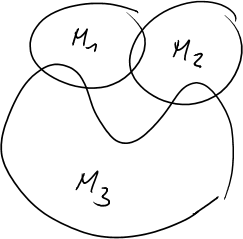
\includegraphics[width=4cm]{Bilder/178}\\
		$M_1\cap M_2\ne\emptyset$\\
		$M_1\cap M_2\cap M_3=\emptyset$
		\caption{}
	\end{minipage}
	\begin{minipage}{0.32\linewidth}
		\centering 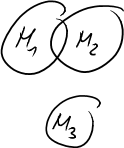
\includegraphics[width=2cm]{Bilder/179}\\
		$M_1\cap M_2\ne\emptyset$\\
		$M_1\cap M_2\cap M_3=\emptyset$
		\caption{}
	\end{minipage}
	\begin{minipage}{0.32\linewidth}
		\centering 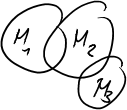
\includegraphics[width=2.1cm]{Bilder/180}\\
		$M_1\cap M_2\ne\emptyset$\\
		$M_1\cap M_2\cap M_3=\emptyset$
		\caption{}
	\end{minipage}
\end{figure}

\clearpage
\Satz{Für endliche Mengen $M,N$ gilt:
	\begin{enumerate}
		\item\label{m1} \redframe{$|M\cup N|=|M|+|N|-|M\cap N|$}\\
		sind $M$ und $N$ disjunkt, so gilt $|M\cup N|=|M|+|N|$ (Umkehrung gilt ebenso; als Beweis für disjunkt)\\
		\\
		\blue{\ul{\black{Subaditivität:}}}\\
		$\left|\bigcup\limits_{i=1}^rM_i\right|\le\sum\limits_{i=1}^{r}|M_i|$\\
		$|M_1\cup\ldots\cup M_r|\le|M_1|+\ldots+|M_r|$\\
		Gleichheit gilt genau dann, wenn $M_1,\ldots,M_r$ paarweise disjunkt sind.
		
		\item\label{m2} Für $M\subseteq N$ gilt: \redframe{$|N\setminus M| = |N|-|M|$}
		\item\label{m3} \redframe{$|M\times N| = |M|\cdot|N|$}
	\end{enumerate}}

\Bsp zu \ref*{m1}.
\vspace{-3ex}
\imgw{Bilder/181}{}{}{4.5cm}
\vspace{-3ex}
\begin{align*}
M&=\{1,2,3,4\}&|M|=4\\
N&=\{3,4,5,6,7,8\}&|N|=6\\
M\cup N&=\{1,2,3,4,5,6,7,8\}&|M\cup N|=8\\
M\cap N&=\{3,4\}&|M\cap N|=2\\
|M\cup N|&=|M|+|N|-|M\cap N|\\
8&=4+6-2\\
\end{align*}

\Bsp zu \ref*{m2}.
\vspace{-3ex}
\imgw{Bilder/182}{}{}{5cm}
\vspace{-8ex}
\begin{align*}
N&=\{1,2,3,4,5\}\\
M&=\{3,4,5\}\\
N\setminus M&=\{1,2\}\\
\end{align*}
sind $M,N$ beliebig, so gilt: \redframe{$|N\setminus M|=|N|-|M\cap N|$},\\
da $N\setminus M = N\setminus(M\cap N)$ und $M\cap N\subseteq N$.

\Bsp zu \ref*{m3}.
\vspace{-3ex}
\imgw{Bilder/183}{}{}{8cm}
\vspace{-8ex}
\begin{align*}
|M|&=2\\
|N|&=3\\
|M\times N| &= 6 = 2\cdot 3 = |M|\cdot|N|\\
\end{align*}
$\left|\bigX\limits_{i=1}^rM_i\right|=\prod\limits_{i=1}^r|M_i|$\\
$|M_1\times\ldots\times M_r|=|M_1|\cdot\ldots\cdot|M_r|$

\Theorem{{\bf Prinzip der Inklusion und Exklusion, Siebformel}\\
	\\
	\Redbox{$|M_1\cup\ldots\cup M_r|=\sum\limits_{k=1}^{r}(-1)^{k-1}\sum\limits_{1\le i_1<\ldots<i_k\le r}\left|\bigcap\limits_{\nu=1}^kM_{i_\nu}\right|\\
		\textcolor{red!15}{|M_1\cup\ldots\cup M_r|}=\sum\limits_{k=1}^{r}(-1)^{k-1}\sum\limits_{1\le i_1<\ldots<i_k\le r}\left|M_{i_1}\cap\ldots\cap M_{i_k}\right|$}}

\Bsps
\begin{enumerate}
	\item $r=3$
	\begin{align*}
	|M_1\cup M_2\cup M_3| =\ &\red{\underbrace{\black{|M_1|+|M_2|+|M_3|}}_{k=1}}\\
	&\red{\underbrace{\black{-|M_1\cap M_2|-|M_1\cap M_3|-|M_2\cap M_3|}}_{k=2}}\\
	&\red{\underbrace{\black{+|M_1\cap M_2\cap M_3|}}_{k=3}}
	\end{align*}
	
	\item $r=4$
	
	$|M_1\cup M_2\cup M_3\cup M_4| = \red{\underbrace{\black{|M_1|+|M_2|+|M_3|+|M_4|}}_{k=1}}\\
	\red{\underbrace{\black{-|M_1\cap M_2|-|M_1\cap M_3|-|M_1\cap M_4|-|M_2\cap M_3|-|M_2\cap M_4|-|M_3\cap M_4|}}_{k=2}}\\
	\red{\underbrace{\black{+|M_1\cap M_2\cap M_3|+|M_1\cap M_2\cap M_4|+|M_1\cap M_3\cap M_4|+|M_2\cap M_3\cap M_4|}}_{k=3}}\\
	\red{\underbrace{\black{-|M_1\cap M_2\cap M_3\cap M_4|}}_{k=4}}$
	
	Anzahl = $\binom{r}{k}$\\
	$k=1:\binom{4}{1}=4$\qquad
	$k=2:\binom{4}{2}=6$\\
	$k=3:\binom{4}{3}=4$\qquad
	$k=4:\binom{4}{4}=1$
\end{enumerate}

\clearpage
\section{Rechenregeln - Mengenalgebra}

	Die Mengenoperatoren:
	\begin{itemize}
		\item Vereinigung $\cup$
		\item Schnitt $\cap$
		\item Differenz $\setminus$
		\item Komplement $\bar{ }$
		\item Produkt $\times$
	\end{itemize}
	
	genügen gewissen Rechenregeln.
	
	Die Operatoren bilden zusammen mit den Mengen die sogenannte \underline{Mengenalgebra}.

	Rechenregeln: $A,B \subseteq \Omega$
	\begin{enumerate}
		\item $A \cap B = B \cap A$\\
		$A \cup B = B \cup A$
		\hfill{Kommutativität}
		\item $A \cap (B \cap C) = (A \cap B) \cap C$\\
		$A \cup (B \cup C) = (A \cup B) \cup C$
		\hfill{Assoziativität}
		\item $A \cap (B \cup C) = (A \cap B) \cup (A \cap C)$\\
		$A \cup (B \cap C) = (A \cup B) \cap (A \cup C)$
		\hfill{Distributivität}
		\item $A\cap (A\cup B) = A$\\
		$A\cup (A\cap B) = A$
		\hfill{Absorption}
		\item $A\cap A = A$\\
		$A\cup A = A$
		\hfill{Idempotenz}
		\item $\ol{\ol A} = A \hspace{40pt} (\ol A = \Omega \setminus A)$
		\item $\ol{A\cap B} = \ol A \cup \ol B$\\
		$\ol{A\cup B} = \ol A \cap \ol B$
		\hfill{Gesetze von de Morgan}
		\item $A \cup \emptyset = A, \hspace{40pt} A\cap \Omega = A$\\
		$A \cap \emptyset = \emptyset, \hspace{40pt} A\cup \Omega = \Omega$
		\hfill{Neutralität}
		\item $A \cap \ol A = \emptyset, \hspace{40pt} A\cup \ol A = \Omega$
		\Beachte $(A,B \subseteq \Omega, \ol B = \Omega \setminus B)$
		
		$A\setminus B = A \cap \ol B$
	\end{enumerate}
	
	\Bsps
	\begin{enumerate}
		\item Zeigen Sie $M \Delta N = (M\cup N)\setminus(M\cap N)$

		$M\Delta N = (M\setminus N) \cup (N \setminus M)$
		
		\vspace{-0.6cm}
		\begin{align*}
			(M \cup N)\setminus(M\cap N)&= (M\cup N)\cap\ol{(M\cap N)}\\
			&= (M\cup N)\cap(\ol M \cup \ol N)\\
			&= [(M\cup N) \cap \ol M]\cup[(M\cup N)\cap \ol N]\\
			&= [\underbrace{(M \cap \ol M)}_\emptyset \cup (N\cap \ol M)]\cup[(M\cap \ol N)\cup \underbrace{(N \cap \ol N)}_\emptyset]\\
			&= [N\cap \ol M] \cup [M \cap \ol N]\\
			&= (N\setminus M)\cup(M\setminus N)\\
			&= (M\setminus N) \cup (N\setminus M)\\
			&= M\Delta N
		\end{align*}

		\item Vereinfachen Sie $\ol{A\cap \ol B}\cup(B\cap C)$
		
		\begin{align*}
			\ol{A\cap \ol B}\cup(B\cap C) &= (\ol A \cup B) \cup (B\cap C)\\
			&= \ol A \cup [\underbrace{B \cup (B\cap C)}_B]\\
			&= \ol A \cup B
		\end{align*}
	\end{enumerate}

\clearpage
\section{Relationen und Abbildungen/Funktionen}

\subsection{Relationen}

\Def $M,N$ Mengen

Eine (binäre) Relation auf $M\times N$ ist eine Teilmenge $R\subseteq M\times N$; ist $M =N$, so heißt $R$ Relation auf $M$.

Statt $(x;y) \in R$ schreibt man auch $xRy$

$R$ ist eine Menge von Paaren $(x;y); x \in M, y \in N;$ ist $(x;y) \in R$, so stehen $x$ und $y$ in Relation (bezüglich $R$) zueinander.

\Bsps

\imgw{Bilder/0}{Beispiel-Relation}{abbR}{8cm}

\begin{enumerate}
	\item In Abbildung \ref{abbR} ist folgende Relation gezeigt:
	
	$R=\{(A;a), (A;b), (A;c), (B;b), (C;a), (D;a), (D;c)\}$
	
	\item Ordnungsrelation $R_\leq$ auf $\R$
	
	$R_\leq = \{(x;y)\mid x,y \in \R$ und $x \leq y\}$
	
	statt $xR_\leq y$ schreibt man $x\leq y$
	
	\item Teilmengenrelation $R_\subseteq$ auf $\mathcal{P}(M)$ ($M$ Menge)
	
	$R_\subseteq = \{(A;B)\mid A,B \subseteq M, A\subseteq B\}$
	
	statt $AR_\subseteq B$ schreibt man $A\subseteq B$
	
	\item Teilbarkeitsrelation $R_\mid$ auf $\N$
	
	$R_\mid = \{(u;m)\mid n,m \in \N\ n\mid m\}$\\
	{\flqq $n$ teilt $m$\frqq} bzw. {\flqq $m$ ist durch $n$ teilbar\frqq}
	
	\item Elementrelation $R_\in$ auf $M\times \mathcal{P}(M)$
	
	$R_\in = \{(x, A)\mid x\in M, A\in \mathcal{P}(M) \text{ und } x\in A\}$
	
	statt $xR_\in M$ schreibt man $x \in M$.
	
	\Bem Zu einer Relation definiert man i.d.R. ein Relationszeichen $\square$ und schreit $x \square y$ statt $xRy$
	
	\Def $R$ sei eine Relation auf einer Menge $M$. Dann heißt $R$
	\begin{itemize}
		\item reflexiv, wenn $xRx$
		\item symmetrisch, wenn $xRy \Rightarrow yRx$
		\item antisymmetrisch, wenn $xRy\text{ und }yRx \Rightarrow x=y$
		\item transitiv, wenn $xRy\text{ und }yRz \Rightarrow xRz$
	\end{itemize}
		
		für alle $x,y,z \in M$ gilt.
		
\end{enumerate}

\Satz{Die Ordnungsrelation $R_\leq$ auf $\R$ ist reflexiv, antisymmetrisch und transitiv.}

\Def Eine Relation $\preceq$ auf einer Menge $M$, die reflexiv, antisymmetrisch und transitiv ist, heißt partielle Ordnung auf $M$; die Menge $M$ heißt dann partiell geordnet.

Sind je zwei Elemente $x, y \in M$ bezüglich $\preceq$ vergleichbar, so heißt $\preceq$ totale (lineare, vollständige) Ordnung auf $M$ und $M$ heißt total geordnet.

\Bsps
\begin{enumerate}
	\item $\leq$ auf $\R$ ist eine totale Ordnung
	\item $\subseteq$ auf $\mathcal{P}(M)$ ist eine partielle Ordnung, die i.a. nicht total ist.
	
	$M = \{1,2\}$
	
	$\mathcal{P}(M) = \{\emptyset, \underbrace{\{1\}}_{A}, \underbrace{\{2\}}_{B}, \{1,2\}\}$
	
	$A\nsubseteq B$ und $B \nsubseteq A \Longrightarrow$ keine totale Ordnung (nur partiell)
\end{enumerate}

\emph{Hasse-Diagramm}

\imgw{Bilder/1}{Hasse-Diagramm}{hasseDiagramm}{4cm}

\Def Eine Relation $R$ auf einer Menge $M$ heißt Äquivalenzrelation, wenn $R$
\begin{itemize}
	\item reflexiv
	\item symmetrisch
	\item transitiv
\end{itemize}

ist. Statt $xRy$ schreibt man auch $x\sim_R y$ oder einfach $x\sim y$, falls $R$ {\flqq klar ist\frqq}.

Für $x \in M$ heißt
$[x] = \{y\mid y\in M\text{ und }y\sim x\}$

Äquivalenzklasse von $x$, und $x$ heißt Vertreter oder Repräsentant der Äquivalenzklasse $[x]$.

\Bsps
\begin{enumerate}
	\item Auto1 $\sim$ Auto2 $\Longleftrightarrow$ Auto1 hat dieselbe Farbe wie Auto2
	\item Geraden $g,h$: $g\sim h \Longleftrightarrow g\|h$
	\item Definiere Relation $\sim_n (n\in \N)$ auf $\N$
	
	$x\sim_n y : \Longleftrightarrow n\mid (x-y)$, d.h. $x-y$ ist durch $n$ teilbar ({\flqq $n$ teilt $x-y$\frqq})
	
	$\sim_n$ ist eine Äquivalenzrelation
\end{enumerate}

\Satz{Sei $M$ eine Menge und $\sim$ eine Äquivalenzrelation auf $M$.}

\begin{enumerate}[i)]
\item Für $x,y \in M$ gilt:
$[x]\cap[y]\neq\emptyset \Longleftarrow[x] = [y]$

(d.h. für beliebige $x,y \in M$ sind die zugehörigen Äquivalenzklassen $[x],[y]$ entweder disjunkt oder gleich)

\item Für jedes $y\in[x]$ gilt $[x] = [y]$, d.h. jedes Element aus $[x]$ ist ein Repräsentant der Äquivalenzklasse $[x]$.

\item Sind $[x_1], [x_2],\ldots$ alle Äquivalenzklassen der Äquivalenzrelation $\sim$, so gilt

$M = \bigcupdot\limits_{i}[x_i] = [x_1] \cupdot [x_2] \cupdot \ldots$

Äquivalenzklassen von $\sim$;

man nennt dann $x_1,x_2,\ldots$ ein vollständiges Repräsentantensystem.

\Bsp

	Äquivalenrelation $x\sim_3 y$ auf $\N$
	
	$x\sim_3 y \Longleftrightarrow 3\mid (x-y)$
	
	Äquivalenzklassen $[0],[1],[2]$
	
	Daher ist $0,1,2$ ein vollständiges Repräsentantensystem von $\sim_3$
	
	Statt $x\sim_3y$ schreibt man auch $x \equiv y \mod 3$
	
	{\flqq $x$ ist kongruent zu $y$ modulo $3$\frqq}
	
	$x\sim_3y \Longleftrightarrow x\text{ und }y$ haben bei Division durch $3$ den selben Rest.
	
	$x=3a+r \hspace{40pt} 0\leq r \leq 2$\\
	$y=3b+s \hspace{40pt} 0\leq s \leq 2$
	
	$x-y = 3a+r-3b-s\\
	x-y = 3(a-b)+(r-s)\\
	\underbrace{\underbrace{x-y}_\text{durch drei teilbar}-3(a-b)}_\text{durch drei teilbar}=\underbrace{r-s}_{-2\leq r-s \leq 2}$
	                             
	$r-s = 0$, d.h. $r=s$
	
	$\Leftarrow$ ok
	
	$[0],[1],[2]$\\
	$[3],[4],[5]$\\
	$[6],[7],[8]$\\
	$\hspace*{5pt}\vdots\hspace*{14pt}\vdots\hspace*{14pt}\vdots$
\end{enumerate}

\clearpage
\subsection{Abbildungen/Funktionen}
\Def $M,N$ Mengen

\begin{enumerate}
	\item Eine Abbildung/Funktion $f$ von $M$ nach $N$ ist eine Relation $R_f \subseteq M\times N$, so dass gilt:\\
	zu jedem $x\in M$ gibt es genau ein $y\in N$\\
	mit $(x,y)\in R_f$
	
	i.Z. $f:M\to N,x\mapsto f(x)$ (bzw. $M \stackrel{f}{\to} N$)
	
	\imgw{Bilder/10}{}{}{7cm}
	
	$x$: Dummy-Variable (Platzhalter für den {\flqq Eingang\frqq} der Funktion)
	
	Das durch $x\in M$ eindeutig bestimmte $y\in N$ mit $(x,y)\in R_f$ wird mit $f(x)$ bezeichnet (d.h. $y=f(x)$) und heißt das Bild von $x$ unter $f$ oder Funktionswert von $f$ in $x$; $x$ heißt Urbild von $y=f(x)$
	
	\item Ist $f:M\to N$ eine Abbildung, so heißt
	\begin{enumerate}
		\item $D_f = D(f):=M$ \hfill Definitionsmenge/-bereich von $f$
		\item $N$ \hfill Ziel- oder Wertemenge
		\item $f(M)=\{f(x)\mid x\in M\}$ \hfill Bildmenge/Bild von $f$
		
		allgemein in $A\subseteq M$ heißt $f(A)=\{f(x)\mid x\in A\}$ das Bild/Bildmenge von $A$ unter $f$
		\item $G_f=\{(x,y)\mid x\in M, y=f(x)\}\quad(=R_f)$
		\hfill Graph von $f$
	\end{enumerate}
\end{enumerate}

\Bsps

\begin{enumerate}
	\item $f:\{1,2,3,4\} \to \{a,b,c,d,e\}$
	
	$1\mapsto a$\qquad $f(1)=a$\\
	$2\mapsto a$\qquad $f(1)=a$\\
	$3\mapsto c$\qquad $f(1)=c$\\
	$4\mapsto b$\qquad $f(1)=b$\\
	$x\mapsto f(x)$
			
	$D(f)=\{1,2,3,4\}$
	
	\imgw{Bilder/11}{}{}{10cm}
	
	$a$ ist Bild von $1$ unter $f$\qquad $1$ ist Urbild von $a$ unter $f$\\
	$a$ ist Bild von $2$ unter $f$\qquad $2$ ist Urbild von $a$ unter $f$\\
	$c$ ist Bild von $3$ unter $f$\qquad $3$ ist Urbild von $c$ unter $f$\\
	$b$ ist Bild von $4$ unter $f$\qquad $4$ ist Urbild von $b$ unter $f$
	
	\Beachte Zuordnungen der Form
	
	$x\mapsto y_1\qquad x\mapsto y_2\qquad (y_1 \ne y_2)$
	
	sind bei Abbildungen verboten (bei Relationen jedoch erlaubt)
	
	$G_f = \{(1,a),(2,a),(3,c),(4,b)\}$
	
	Bild von $f: f(M)=\{f(1),f(2),f(3),f(4)\} = \{a,b,c\}$
	
	\item $f:\R\to\R, x\mapsto x^2 (=f(x))$
	
	\imgw{Bilder/12}{}{}{7cm}
	
	$D(f) = \R$\\
	$f(\R)=\Rop$
	
	$g:\Rop\to\R, x\mapsto x^2 (=g(x))$
	
	\imgw{Bilder/13}{}{}{7cm}
	
	$D(g) = \Rop$\\
	$g(\Rop)=\Rop$
	
	
	$h:\Rop\to\Rop, x\mapsto x^2 (=h(x))$
	
	\imgw{Bilder/13}{}{}{7cm}
	Graph wie bei $g$
	
	$D(h) = \Rop$\\
	$h(\Rop)=\Rop$
	
	$f\ne g, f\ne h, g\ne h$
	
	$k:[-1;1]\to\R, x\mapsto x^2 (=k(x))$
	
	\imgw{Bilder/14}{}{}{7cm}
	
	$D(k) = [-1;1]$\\
	$k([-1;1])=[0;1]$
	
	\item $f:\No \to \{0,1,2,\ldots,n-1\}$
	
	$x\mapsto x \mod n$ (=Rest der Division $x:n$) \hfill Hashfunktion
	
	\item $g:\R\times\R\to\R, (x,y)\mapsto x\cdot y$
	
	$D(g)=\R\times\R = \R^2$\\
	$g(\R^2) = \R$
\end{enumerate}

\Def (Komposition von Abbildungen)

Sind $f:L\to M$ und $g:M\to N$ Abbildungen, so ist auch\\
\redbox{$h:L\to N, x\mapsto g(f(x)) (=h(x))$}\\
eine Abbildung, $h$ heißt Komposition (Verkettung, Hintereinanderausführung) von $f$ und $g$\\
i.Z. $h=g\circ f$ (sprich: {\flqq $g$ nach $f$\frqq})

$L\stackrel{f}{\to}M\stackrel{g}{\to}N$\\
$g\circ f$

$(g\circ f)(x) = g(f(x))$

\Bem Damit die Komposition $g\circ f$ gebildet werden kann, muss\\
$f(L)\subseteq D_g$\\
Ausgang von $f$ $\subseteq$ Eingang von $g$\\
Bild von $f$ $\subseteq$ Definitionsmenge von $g$

\Bsp
\ \\
$f:\R\to\R, x\mapsto x^2$ \qquad $f(\R) = \Rop$\\
$g:\Rop\to\R, x\mapsto \sqrt{x}$ \qquad $D_g=\Rop$\\
$f(\R)\subseteq D_g$

$g\circ f: \R\to\R, x\mapsto (g\circ f)(x)=g(f(x))=g(x^2)=\sqrt{x^2}$

\Def Eine Abbildung $f:M\to N$ heißt
\begin{itemize}
	\item injektiv, wenn für alle $x_1,x_2\in M, x_1\ne x_2$ gilt: $f(x_1)\ne f(x_2)$
	\item surjektiv, wenn es für jedes $y\in N$ ein $x\in M$ mit $y=f(x)$ gibt
	\item bijektiv, wenn $f$ injektiv und surjektiv ist
\end{itemize}

\Bem $f$ ist

\begin{itemize}
	\item nicht injektiv, wenn $x_1\mapsto y, x_2\mapsto y$
	für gewisse $x_1\ne x_2$ gilt.
	
	\item nicht surjektiv, wenn gewisse $y\in N$ {\flqq übrigbleiben\frqq}
	
	\imgw{Bilder/15}{}{}{9cm}
	
	\greenbox{$f(M)$}$\ne N$
\end{itemize}

\clearpage
\Bsps

\imgw{Bilder/16}{injektiv, aber nicht surjektiv}{}{7cm}
\imgw{Bilder/17}{surjektiv, aber nicht injektiv}{}{7cm}
\imgw{Bilder/18}{injektiv und surjektiv, also bijektiv}{}{7cm}

\clearpage
\Def Ist $f:M\to N$ bijektiv, so existiert die Umkehrabbildung/-funktion

$\inv{f}:N\to M$

für diese gilt:

\redbox{$x=\inv{f}(y)\Leftrightarrow f(x)=y$}

Ist $f$ nicht bijektiv, so existiert auch keine Umkehrabbildung.

\Satz{Ist $f:M\to N$ bijektiv und $\inv{f}:N\to M$ die Umkehrabbildung, so gilt:
	\begin{enumerate}
		\item $\inv{f}\circ f = id_M$ \label{refa}
		\item $f\circ \inv{f} = id_N$ \label{refb}
	\end{enumerate}
	wobei ${id}_M:M\to M, x\mapsto x$ und ${id}_N:N\to N, y\mapsto y$ die sogenannten identischen Abbildungen sind.
}

\Bem \quad \\
zu \ref*{refa}: $(\inv{f}\circ f)(x) = \inv{f}(f(x))={id}_M(x)=x$\\
zu \ref*{refb}: $(f\circ \inv{f})(y) = f(\inv{f}(y))={id}_N(y)=y$

($f$ und $\inv{f}$ {\flqq löschen sich gegenseitig aus\frqq})

\Satz{Für $M,N\subseteq \R$ gilt:\\
	\\
	$f:M\to N$ ist genau dann bijektiv, wenn jede Parallele $y=a$ mit $a\in N$ (Parallele schneidet y-Achse bei $a$) den Graph von $f$ genau einmal schneidet.
}

\imgw{Bilder/19}{}{}{10cm}

\clearpage
\Bsps
\begin{enumerate}
	\item $f:\Rop\to\Rop, x\mapsto x^2$
	
	\imgw{Bilder/20}{}{}{7cm}
	
	$f$ ist bijektiv
	
	Umkehrfunktion
	$\inv{f}:\Rop\to\Rop\\
	x=\inv{f}(y)\Leftrightarrow y=f(x)\\
	y=x^2 \mid {}^{\white{(}+\white{)}}_{(-)}\sqrt{\ } (x\ge 0)\\
	\Leftrightarrow {}^{\white{(}+\white{)}}_{(-)}\sqrt{y} = x (\ge 0)\\
	\Leftrightarrow x=\sqrt{y} = \inv{f}(y)$
	
	$(\inv{f}\circ f)(x)=\inv{f}(f(x))=\inv{f}(x^2)=\sqrt{x^2} = x$ (da $x\ge 0$)
	
	$(f\circ \inv{f})(y)=f(\inv{f}(y))=f(\sqrt{y})=\sqrt{y}^2 = y$
	
	\clearpage
	\item $f:\R\to\R^+, x\mapsto b^x (b>1)$
	
	\imgw{Bilder/21}{}{}{7cm}
	
	$f$ ist bijektiv
	
	$\Rightarrow$ Umkehrfunktion $\inv{f}(y)= \log_b(y)$
	
	$y=b^x=f(x)\Leftrightarrow x=\inv{f}(y) = \log_b(y)$
	
	$(\inv{f}\circ f)(x) = \inv{f}(f(x))= \inv{f}(b^x) = $ \redbox{$\log_b(b^x) = x$}
	
	$(f\circ \inv{f})(y) = f(\inv{f}(y))= f(\log_b(y)) = $ \redbox{$b^{\log_b(y)} = y$}
	
	\clearpage
	\item $f:\{x\ge 1\}\to\{y\ge 1\}, x\mapsto (x-1)^2 + 1$
	
	Scheitelpunktform einer Parabel: $y= a(x-x_s)^2+y_s$\\
	Scheitel $S(x_s\mid y_s)$
	
	\imgw{Bilder/22}{}{}{10cm}
	
	$f$ ist bijektiv
	
	$\Rightarrow$ Umkehrfunktion: $\inv{f}:\{y\ge1\}\to\{x\ge 1\}$
	
	$y=f(x) \Leftrightarrow y=(x-1)^2 + 1\mid -1\\
	\Leftrightarrow y - 1=(x-1)^2 \mid \pm\sqrt{\ }\\
	\Leftrightarrow \pm\sqrt{y-1}=x-1\ (\ge 0)\ (x\ge 1,\text{ d.h. }x-1 \ge 0)\\
	\Leftrightarrow x = \sqrt{y-1} +1\ (= \inv{f}(y))$
	
	\clearpage
	\item $g:\{x\le 1\} \to \{y\ge 1\} , x\mapsto (x-1)^2+1$
	
	Prüfe, ob $g$ bijektiv ist und bestimme ggf. $\inv{g}$!
	
	\imgw{Bilder/24}{}{}{10cm}
	
	$g$ ist bijektiv
	
	$\Rightarrow$ Umkehrfunktion $\inv{g}:\{y\ge 1\}\to\{x\le 1\}$
	
	\begin{align*}
		y=g(x) \Leftrightarrow y&=(x-1)^2+1\mid -1\\
		y-1 &= (x-1)^2\mid \pm\sqrt{\ }\\
		\pm\sqrt{y-1} &= x-1\ (\le 0)\ (x \le 1,\text{ d.h. }x-1 \le 0)\\
		x &= -\sqrt{y-1}+1
	\end{align*}
\end{enumerate}

\clearpage
\Def Ist $f:M\to N, x \mapsto f(x)$ eine Abbildung und $D\subseteq M$ eine Teilmenge, so heißt\\
${f|}_{D}:D\to N, x\mapsto f(x)$\\
die Einschränkung von $f$ auf $D$.

\Bem Ist $f$ nicht injektiv, so ist oftmals die Einschränkung ${f|}_{D}$ auf eine geeignete Teilmenge $D$ injektiv.

(Einschränkung der Zielmenge {\flqq liefert Surjektivität\frqq})

\Bsp 

\imgw{Bilder/23}{}{}{8cm}

${f|}_{D} :D\to N$ ist bijektiv


\clearpage
\chapter{Die komplexen Zahlen}

\section{Definition und Rechenregeln}

\Problem Die quadratische Funktion $f(x)=x^2 +1$ hat in $\R$ keine Nullstelle.\\$(x^2+1>0)$

formal:
\begin{align*}
	x^2+1 &= 0\\
	x^2 &= -1\\
	x_{1/2} &= \pm\sqrt{-1}\in \R
\end{align*}

Kann man den Zahlenbereich $\R$ derart erweitern, dass $x^2+1$ darin eine Nullstelle hat?

\subsection{Konstruktion der komplexen Zahlen}
\ \\
Definiere auf der Menge $\R^2=\R\times\R=\{(x,y)\mid x,y\in\R\}$ wie folgt Addition und Multiplikation:

Für $z_1 = (x_1,y_1)$ und $z_2=(x_2,y_2)$ sei

\vspace{-7ex}
\begin{align*}
	z_1 + z_2 = (x_1,y_1)+(x_2,y_2)&:=(x_1+x_2\ ,\ y_1+y_2)\\
	z_1 \cdot z_2 = (x_1,y_1)\cdot(x_2,y_2)&:=(x_1x_2-y_1y_2\ ,\ x_1y_2+x_2y_1)
\end{align*}

\vspace{-6ex}
\Def $\R^2$ zusammen mit obiger Definition von Addition und Multiplikation erfüllen die Gesetze eines sogenannten Zahlenkörpers (oder Körpers); man schreibt hierfür $\R^2 = \C$ und nennt $\C$ (den Körper der) komplexen Zahlen;\\
für $z=(x,y)\in \C$ heißt\\
$x= \Re(z)$ der Realteil {\tiny(Re$(z)$)}\\
$y= \Im(z)$ der Imaginärteil {\tiny(Im$(z)$)}\\
von $z$.

\subsection{Gesetze eines (Zahl-)Körpers (Körperaxiome)}
\begin{enumerate}
	\item $a + b = b + a\\a \cdot b = b \cdot a$ \hfill Kommutativgesetze
	\item $a+(b+c)=(a+b)+c\\a\cdot (b\cdot c)=(a\cdot b)\cdot c$ \hfill Assoziativgesetze
	\item $a\cdot(b+c)= ab+ac$ \hfill Distributivgesetz
	\item Es existiert ein Element $0$ mit $a+0= 0+a = a$ für jedes $a$\\
	\parbox{0ex}{}\hfill (Existenz eines additiven neutralen Elements)
	\item Es existiert ein Element $1$ mit $a\cdot 1 = 1\cdot a = a$ für jedes $a$\\
	\parbox{0ex}{}\hfill (Existenz eines multiplikativen neutralen Elements)
	\item Zu jedem $a$ gibt es ein Element $-a$ mit $a + (-a) = (-a) + a = 0$\\
	\parbox{0ex}{}\hfill (Existenz eines additiven inversen Elements)
	\item Zu jedem $a\ (a \ne 0)$ gibt es ein Element $\inv{a}\ (=\frac{1}{a})$ mit $\inv{a} \cdot a = a \cdot \inv{a} = 1$\\
	\parbox{0ex}{}\hfill (Existenz eines multiplikativen inversen Elements)
\end{enumerate}

Die Abbildung $\R\to\C;c\mapsto(x;0)$ ist injektiv und verträglich mit den Additionen und Multiplikationen in $\R$ und $\C$.

\begin{align*}
(x_1;0)+(x_2;0) &= (x_1+x_2;0)\\
(x_1;0)\cdot(x_2;0) &= (x_1\cdot x_2;0)\\
\end{align*}

$\Rightarrow$ Betrachte $\R$ als Teilmenge von $\C\ (\R\subseteq\C)$
\begin{align*}
\R &\subseteq \C\\
x &\entspricht (x;0)\\
\R &= \{z\in\C\mid\Im{z}=0\}
\end{align*}

\Def Die imaginäre Zahl $\i\in\C$ ist definiert durch $\i=(0;1)$

\Beh 
\begin{align*}
\i^2 &= -1\\
&=(0;1)\cdot(0;1)\\
&= (0-1;0\cdot 1 + 1\cdot 0)\\
&= (-1;0)\\
&= -1
\end{align*}

\Satz{{\bf kartesische Darstellung}\\
	\\
	Jede komplexe Zahl $z\in\C$ kann \underline{eindeutig} geschrieben werden in der Form\vspace{1ex}\\
	\redbox{$z= x+\i\cdot y$} $(x,y\in\R)$\vspace{1ex}\\
	es gilt $x=\Re{z}$ und $y=\Im{z}$
}

\Beweis 
\begin{align*}
z&=(x;y)\\
x+\i y &= (x;0)+(0;1)\cdot(y;0)\\
&= (x;0) + (0\cdot y-1\cdot 0; 0\cdot 0+1\cdot y)\\
&= (x;0) + (0; y)\\
&= (x;y)\\
&= z
\end{align*}

\paragraph{Geometrische Interpretation} (Gaußsche Zahlenebene)

$z=x+\i y \entspricht \text{ Punkt } P(x;y)\text{ bzw. Vektor }\vec{v}=\binom{x}{y}$

%bild 1
\imgw{Bilder/25}{}{}{11cm}

\Bsps
\begin{enumerate}
	\item $-2+3\i+4-8\i\\
	= 2-5\i$
	
	\item $(-2+3\i)\cdot(4-8\i)\\
	= -8 +16\i+12\i-24\underbrace{\i^2}_{-1}\\
	= -8+28\i+24\\
	= 16+28\i$
	
	\item $(-2+3\i)^2=(-2)^2+2\cdot(-2)\cdot3\i+(3\i)^2\\
	=4-12\i+3^2\underbrace{\i^2}_{-1}\\
	=4-12\i-9\\
	=-5-12\i$
\end{enumerate}

\clearpage
\section{Operationen auf komplexen Zahlen}
\subsection{Komplex-Konjugation}

\Def Für eine komplexe Zahl $z = x+\i y$ heißt\vspace{1ex}\\
\redbox{$\ol{z}=x-\i y$}\vspace{1ex}\\
die \underline{Komplex-Konjugierte} von $z$; die Abbildung $\ol{\color{white}z}:\C\to\C,z\mapsto \ol{z}$ heißt \underline{Komplex-Konjugation}.

\paragraph{Geometrische Interpretation:}
$\ol{z}$ entsteht aus $z$ durch Spiegelung an der reellen Achse.

%bild 2
\imgw{Bilder/26}{}{}{9cm}

\clearpage
\Satz{{\bf Eigenschaften der Komplex-Konjugation}
	\begin{enumerate}
		\item $\ol{\ol{z}} = z$
		\item $\ol{z_1\pm z_2} = \ol{z_1}\pm\ol{z_2}$
		\item $\ol{z_1\cdot z_2} = \ol{z_1}\cdot\ol{z_2}$
		\item $\ol{\left(\dfrac{z_1}{z_2}\right)} = \dfrac{\ol{z_1}}{\ol{z_2}}$
		\item $\Re(z)={1\over 2}(z + \ol{z})$
		\item $\Im(z)={1\over 2\i}(z - \ol{z})$
		\item $z\in\R \Longleftrightarrow z = \ol{z}$
		\item $z\in \i\R \Longleftrightarrow z = -\ol{z}$
	\end{enumerate}
}

\Beweis HÜ

\begin{enumerate}
	\item $z=x+\i y, \ol{z}=x-\i y, \ol{\ol{z}}=x-(-\i y) = x+\i y = z$
	\item %Bild 3
	%continue
	$z_1=x_1+\i y_1, z_2=x_2+\i y_2$\\
	$\ol{z_1}=x_1-\i y_1, \ol{z_2}=x_2-\i y_2$
	
	\begin{align*}
	\ol{z_1+z_2}&=\ol{(x_1+\i y_1)+(x_2+\i y_2)}\\
	&=\ol{x_1+x_2+\i(y_1+y_2)}\\
	&=x_1+x_2-\i(y_1+y_2)\\
	\ol{z_1}+\ol{z_2}&=(x_1-\i y_1)+(x_2-\i y_2)\\
	&=x_1+x_2-\i y_1-\i y_2\\
	&=x_1+x_2-\i(y_1+y_2)
	\end{align*}
\end{enumerate}

\Bsps \ 
\begin{enumerate}
	\item $\ol{\ol{4+3\i}} = \ol{4-3\i} = 4+3\i$
	\item $\ol{(7-3\i)+(-8+5\i)} = \ol{(7-3\i)}+\ol{(-8+5\i)}\\
	= 7+3\i+(-8-5\i)\\
	=7+3\i-8-5\i\\
	=-1-2\i$
	\item $\ol{\i} = \ol{0+\i}=0-\i=-\i$
	\item $\ol{(1-2\i)\cdot(2-3\i)} = \ol{(1-2\i)}\cdot\ol{(2-3\i)}\\
	= (1+2\i)(2+3\i)\\
	= 2+3\i+4\i+6\i^2\\
	= 2+7\i-6\\
	= -4+7\i$
	\item $\Re(5-2\i)=5; \Im(5-2\i)=-2$
	
	\begin{align*}
		\dfrac{1}{2}(z+\ol{z}) &= \dfrac{1}{2}(5-2\i+5+2\i)\\
		&= \dfrac{1}{2}\cdot 10\\
		&= 5\\
		\\
		\dfrac{1}{2\i}(z-\ol{z}) &= \dfrac{1}{2\i}(5-2\i-(5+2\i))\\
		&= \dfrac{1}{2\i}(5-2\i-5-2\i)\\
		&= \dfrac{1}{2\i}(-4\i)\\
		&= -\dfrac{4\i}{2\i}\\
		&= -2
	\end{align*}
\end{enumerate}

\clearpage
\subsection{Betrag}

\Def Für $z=x+\i y\in\C$ heißt\\
$|z| =\sqrt{x^2+y^2}=\sqrt{z\cdot \ol{z}}$\\
der \underline{Betrag} von $z$.

\Bem Im Spezialfall $z = x\in\R$ gilt\\
$|z| =\sqrt{x^2}=|x|$\\
neue Definition des Betrags einer komplexen Zahl \space {\flqq alte Definition\frqq} des Betrags einer reellen Zahl

\paragraph{Geometrische Interpretation des Betrags:}

%bild 4
\imgw{Bilder/27}{}{}{9cm}

$z=2+3\i \entspricht\text{ Punkt }P(2;3)\\
\text{bzw. Vektor }\vec{v}=\binom{2}{3}$

$|z|$ = Abstand von P zum Ursprung\\
= Länge des Vektors $\vec{v}$

\Bsps
\begin{enumerate}
	\item $|2+3\i| = \sqrt{2^2+3^2} = \sqrt{4+9} = \sqrt{13}$
	\item $|-4+5\i| = \sqrt{(-4)^2+5^2} = \sqrt{16+25} = \sqrt{41}$
	\item $|\i| = \sqrt{0^2+1^2} = \sqrt{1} = 1$
\end{enumerate}

\Bem $z= x+\i y$\\
$z\cdot \ol{z} =(x+\i y)(x-\i y)=x^2-(\i y)^2 = x^2 -\i^2y^2= x^2 -(-y^2)= x^2+y^2$

$=\dfrac{1}{z}\cdot\dfrac{\ol{z}}{\ol{z}}=\dfrac{\ol{z}}{z\ol{z}}=\dfrac{\ol{z}}{x^2+y^2}=\dfrac{\ol{z}}{{|z|}^2}$

$x^2+y^2={|z|}^2$

\Bem i.a. ist ${|z|}^2\neq|z^2|$


%2014_10-27
\clearpage
\subsection{Multiplikativ Inverses}

\Satz{{\bf Formel für multiplikatives Inverses}\\
	\\
	Für $z= x+\i y\in\C,z\neq 0$ gilt:\vspace{1ex}\\
	\redbox{$\inv{z}=\dfrac{1}{z}= \dfrac{\ol{z}}{{|z|}^2} = \dfrac{\ol{z}}{x^2+y^2}$}
}

%\Beweis Idee: {\flqq $\frac{1}{z}$ mit $\ol{z}$ erweitern\frqq}

%$\inv{z}= \dfrac{1}{z}= \dfrac{\ol{z}}{{|z|}^2}$

%\Satz{{\bf Formel für multiplikatives Inverses}\\
%	\\
%	Für $z\in\C,z\neq 0$ gilt $(c=x+\i y)$\vspace{1ex}\\
%	\redbox{$\inv{z}= \dfrac{1}{z}= \dfrac{\ol{z}}{{|z|}^2}= \dfrac{\ol{z}}{x^2+y^2}$}}

\Beweis {\flqq mit $\ol{z}$ erweitern\frqq}

%Formel 1
$\inv{z}=\dfrac{1}{z}=\dfrac{\ol{z}}{z\cdot \ol{z}}=\dfrac{\ol{z}}{x^2+y^2}=\dfrac{\ol{z}}{{|z|}^2}$

\begin{align*}
z\cdot \ol{z} &= (x+\i y)(x-\i y) \\
&= x^2-\i xy+\i xy-\i ^2y^2 \\
&= x^2+y^2
\end{align*}

\Bsps
\begin{enumerate}
	\item $\inv{\i }=\dfrac{1}{\i }=\dfrac{\ol{\i }}{\i \cdot\ol{\i }}=\dfrac{-\i }{x^2+y^2}=\dfrac{-\i }{0^2+1^2}=-\i $
	
	\begin{align*}
	\i &=0+1\i\\
	\ol{\i }&= 0-1\i \\
	&= -\i 
	\end{align*}
	
	\paragraph{Probe:} $\dfrac{1}{\i }\i =(-\i )\i = -\i ^2=1$
	
	\item $\inv{(2\i )}=\dfrac{1}{2\i }=\dfrac{\ol{2\i }}{{|2\i |}^2}=\dfrac{-2\i }{0^2+2^2}=\dfrac{-2\i }{4}=-\dfrac{1}{2}\i $
	
	\paragraph{Probe:} $\dfrac{1}{2\i }2\i =(-\dfrac{1}{2}\i )2\i = -\dfrac{1}{2}2\i ^2=1$
	
	\paragraph{Alternative Berechnung:} \quad\\
	$\inv{(2\i )}=\dfrac{1}{2\i }=\dfrac{1}{2}\cdot\dfrac{1}{\i }=-\dfrac{1}{2}\i $
	
	\item $\inv{(1+2\i )}=\dfrac{1}{1+2\i }=\dfrac{1}{1+2\i }\cdot\dfrac{1-2\i }{1-2\i }=\dfrac{1-2\i }{1^2+2^2}=\dfrac{1-2\i }{5}=\dfrac{1}{5}-\dfrac{2}{5}\i $
	
	\paragraph{Probe:} $\dfrac{1}{1+2\i }(1+2\i )=(\dfrac{1}{5}-\dfrac{2}{5}\i )(1+2\i )=\dfrac{1}{5}+\dfrac{2}{5}\i -\dfrac{2}{5}\i -\dfrac{4}{5}\i ^2=\dfrac{1}{5}+\dfrac{4}{5}=1$
\end{enumerate}

\clearpage
\subsection{Inverses und Komplex-Konjugiertes}

\Satz{{\bf Inverses und Komplex-Konjugiertes}\\
	\\
	\redbox{$\ol{\inv{z}}=\ol{\left(\dfrac{1}{z}\right)}=\dfrac{1}{\ol{z}} = \inv{(\ol{z})}$}}

\Beweis 
%Formel 2
$\ol{\inv{z}}=\ol{\left(\dfrac{1}{z}\right)}=\ol{\left(\dfrac{\ol{z}}{{|z|}^2}\right)}=\dfrac{\ol{\ol{z}}}{{|z|}^2}=\dfrac{\ol{\ol{z}}}{{|\ol z|}^2}=\inv{(\ol z)}$

${|z|}^2 = x^2+y^2$\\
${|\ol z|}^2 = x^2+(-y)^2 = x^2+y^2$

\Bem $\ol{\left(\dfrac{z_1}{z_2}\right)}=\ol{\left(z_1\cdot\dfrac{1}{z_2}\right)}=\ol{z_1}\cdot\ol{\left(\dfrac{1}{z_2}\right)}=\ol{z_1}\cdot\dfrac{1}{\ol{z_2}}=\dfrac{\ol{z_1}}{\ol{z_2}}$

\clearpage
\section{Darstellungen komplexer Zahlen}
\subsection{Algebraische (kartesische) Form}

$z=x+\i y$\\
$(x,y \in \R)$

%bild 3
\imgw{Bilder/28}{}{}{9cm}

\clearpage
\subsection{Trigonometrische Form}

Polarkoordinaten $(r;\varphi)$

%bild 4
\imgw{Bilder/29}{}{}{9cm}

$z\neq 0$\\
$r>0, r\in\R$\\
$-\pi<\varphi\leq\pi, \varphi\in\R$

$\dfrac{x}{r} = \cos\varphi \Rightarrow x= r\cos\varphi$\\
$\dfrac{y}{r} = \sin\varphi \Rightarrow y= r\sin\varphi$\\
$z=x+\i y$\\
$\Rightarrow z = x+\i y = r\cos\varphi + \i  r\sin\varphi = r(\cos\varphi+\sin\varphi)$

Polardarstellung (trigonomerische Form)\\
\Redbox{$z = r\cos\varphi + \i  r\sin\varphi = r(\cos\varphi+\sin\varphi)$=}

Kartesische Koordinaten $\leftrightarrow$ Polarkoordinaten\\
$(x,y) \leftrightarrow (r;\varphi)$

\Redbox{
	$x=r\cos\varphi \in \R$\\
	$y=r\sin\varphi \in \R$}

\Redbox{
	$r = \sqrt{x^2+y^2} = |z|$\\
	\\
	$\varphi= \left\{ \begin{array}{ll}
		\arccos(\frac{x}{r}), &\text{falls }y\geq 0 \\
		-\arccos(\frac{x}{r}), &\text{falls }y< 0 \\
		\end{array}\right. $
}

$\varphi = Arg(z) = $ (Hauptwert des) Argument(s) von $z$

$-\pi<\varphi\leq\pi)$

$z = x+\i y$

\paragraph{Polarkoordinaten}
$r=|z|, \varphi=\Arg(z)$

\Bem $(\arccos x)$

%bild 5
\imgh{Bilder/30}{}{}{10.5cm}

\clearpage
\subsection{Eulersche Form}
\redbox{$e^{\i \varphi}=\cos\varphi+\i \sin\varphi$}\qquad (komplexe Exponentialfunktion)

\subsection{Exponentialform}
$z\in\C, z\ne0$

\redbox{$z=r\cdot e^{\i \varphi}$} \qquad\parbox{5cm}{$r=|z|>0\\\varphi=\Arg(z),-\pi<\varphi\leq\pi$}

Folgt aus trigonometrischer Form

$z=r\cdot(\cos\varphi+\i \sin\varphi)$

und der Eulerschen Formel

$e^{\i \varphi}=\cos\varphi+\i \sin\varphi$

\Bem Verwende in der Exponentialform $\varphi$ nur im Bogenmaß (als Vielfaches von $\pi$)

$\xout{z=4e^{\i 30\degree}}\qquad \Rightarrow \qquad e^{\i \frac{\pi}{4}}$

\Bsp $z=2+2\i $\qquad (kartesiche Form)
\imgw{Bilder/31}{}{}{5cm}

\clearpage
Polarkoordinaten $(r;\varphi)$:\\
$r=|z|=\sqrt{2^2+2^2}=\sqrt{8}=2\sqrt{2}$\\
$\varphi = \Arg(z)\qquad y\geq 0\\
=\arccos\left(\dfrac{x}{r}\right)\\
=\arccos\left(\dfrac{2}{2\sqrt{2}}\right)\\
=\arccos\left(\dfrac{1}{2}\sqrt{2}\right)\\
=\dfrac{\pi}{4}$

\begin{tabular}{c|c}
	Gradmaß & Bogenmaß\\
	$\alpha$ & $x$\\
	\hline
	\hline 180$\degree$ & $\pi$ \\ 
	$\alpha$ & $x$ \\ 
\end{tabular} 

\redframe{$\dfrac{\alpha}{180\degree}=\dfrac{x}{\pi}$}

trigonometrische Form\\
$z=2\sqrt{2}(\cos\dfrac{\pi}{4}+\i \sin\dfrac{\pi}{4})$

Exponential Form\\
$z=2\sqrt{2}\cdot e^{\i \frac{\pi}{4}}$

\Satz{{\bf Eigenschaften von $e^{\i \varphi}$}\\
	\\
	$\varphi, \psi\in\R$
	\begin{enumerate}
		\item $e^{\i \varphi}e^{\i \psi}=e^{\i (\varphi+\psi)}$
		\item $e^{-\i \varphi}=\dfrac{1}{e^{\i \varphi}}$
		\item $\left(e^{\i \varphi}\right)^n=e^{\i n\varphi}\qquad(n\in\Z)$
		\item $\left|e^{\i \varphi}\right|=1$\qquad
			\parbox{4cm}{$\Re(e^{\i \varphi})=\cos\varphi\\
			\Im(e^{\i \varphi})=\sin\varphi$}
	\end{enumerate}
}

Durchläuft $\varphi$ das Intervall $[0;2\pi[$ bzw. $]-\pi;\pi]$, so durchläuft $z=e^{\i \varphi}$ alle Punkte auf dem Einheitskreis $|z|=1$.

\Satz{{\bf Satz von de Moivre}\\
	\\
	\redbox{$(\cos\varphi+\i \sin\varphi)^n = \cos(n\varphi)+\i \sin(n\varphi)$}\qquad$(n\in\N,\varphi\in\R)$}

\Beweis\quad\\
$(\cos\varphi+\i \sin\varphi)^n = (e^{\i \varphi})^n = e^{\i n\varphi} = \cos(n\varphi)+\i \sin(n\varphi)$

\paragraph{Anwendungsbeispiel:}
\begin{enumerate}
	\item Es gilt:\\
	\Redbox{$\cos(2\varphi)=\cos^2\varphi-\sin^2\varphi\\
		\sin(2\varphi)=2cos\varphi\sin\varphi$}
	
	\Beweis \quad\\
	\begin{align*}
	\blue{\cos(2\varphi)}+\i \red{sin(2\varphi)}&\stackrel{\text{de Moivre}}{=}(cos\varphi+\i \sin\varphi)^2\\
	&=\cos^2\varphi+2\cos\varphi\i\sin\varphi+\underbrace{(\i\sin\varphi)^2}_{-\sin^2\varphi}\\
	&=\blue{\cos^2\varphi-\sin^2\varphi} +\i \red{2\cos\varphi\sin\varphi}
	\end{align*}
	
	vergleiche die Real- und Imaginärteile\\
	\begin{align*}
	\cos(2\varphi)&=\cos^2\varphi-\sin^2\varphi\\
	\sin(2\varphi)&=2\cos\varphi\sin\varphi
	\end{align*}
	
	\item Additionstheoreme für $\sin(x)$ und $\cos(x)$\\
	\Redbox{$\cos(\varphi + \psi)=\cos\varphi\cos\psi-\sin\varphi\sin\psi\\
		\sin(\varphi + \psi)=\cos\varphi\sin\psi+\sin\varphi\cos\psi$}
	
	\Beweis \quad\\
	\begin{align*}
	\blue{\cos(\varphi + \psi)}+\i\red{\sin(\varphi + \psi)}&=e^{\i(\varphi + \psi)} = e^{\i\varphi}e^{\i\psi}\\
	&=(\cos\varphi + \i\sin\varphi)(\cos\psi + \i\sin\psi)\\
	&=\cos\varphi\cos\psi + \cos\varphi\i\sin\psi + \i\sin\varphi\cos\psi + \ii\sin\varphi\sin\psi\\
	&=\blue{\cos\varphi\cos\psi - \sin\varphi\sin\psi} + \i\red{(\cos\varphi\sin\psi + \sin\varphi\cos\psi)}\\
	\end{align*}
	
	vergleiche die Real- und Imaginärteile\\
	\Beh s.o.
\end{enumerate}

\clearpage
\section{Komplexe Wurzeln}

\Def Sei $w\in\C$. Jede komplexe Zahl $z \in \C$, die die Gleichung $z^n=w$ erfüllt, heißt $n$-te komplexe Wurzel von $w$.

Reelle Zahlen
\begin{align*}
x^n &= a\qquad(a\geq 0)\qquad x\geq 0\\
x&=\sqrt[n]{a}\geq0
\end{align*}

\Satz{
	Zu jedem $0\neq w \in \C$ gibt es genau $n$ verschiedene $n$-te komplexe Wurzeln. Diese sind wie folgt gegeben:\\
	Ist $w=re^{\i \varphi}$ die Exponentialform von $w$, so sind\vspace{1ex}\\
	\redbox{$z_k=r^{\frac{1}{n}}\cdot e^{\i (\frac{\varphi}{n}+\frac{2\pi}{n}k)}$}\qquad $(k=0,1,\ldots,n-1)$\vspace{1ex}\\
	alle $n$-ten komplexen Wurzeln von $w$.
}

Im Spezialfall $w=1$ heißen die Lösungen der Gleichung $z^n=1$ $n$-te (Komplexe) Einheitswurzeln.

\redbox{$\zeta_{k,n} = e^{\i \frac{2\pi}{n}k}$}\qquad $(k = 0,1,2,\ldots, n-1)$

\Beweis \quad
\begin{align*}
(z_k)^n &= \left(r^{\frac{1}{n}}\cdot e^{\i (\frac{\varphi}{n}+\frac{2\pi}{n}k)}\right)^n\\
&= \left(r^{\frac{1}{n}}\right)^n\cdot \left(e^{\i (\frac{\varphi}{n}+\frac{2\pi}{n}k)}\right)^n\\
&= r\cdot e^{\i (\varphi+2\pi k)}\\
&= r\cdot e^{\i \varphi+i2\pi k}\\
&=r\cdot e^{\i \varphi}\cdot e^{\i 2\pi k} =w\\
e^{\i 2\pi k} &= (e^{\i 2\pi})^k = (1)^k =1
\end{align*}
 
\Bem $z_k = r^{\frac{1}{n}}\cdot e^{\i (\frac{\varphi}{n}+\frac{2\pi}{n}k)}\\
 = r^{\frac{1}{n}}\cdot e^{\i \frac{\varphi}{n}}\cdot e^{\i \frac{2\pi}{n}k}\ (k=0,1,\ldots,n-1)\\
 = z_0\cdot e^{\i \frac{2\pi}{n}k}\\
 = z_0\cdot \zeta_{n,k}\\
 $
 \redbox{$z_k=z_0\cdot \zeta_{n,k}$}\\
$z_0$: eine spezielle $n$-te Wurzel von $w$ \\
$\zeta_{n,k}$: $n$-te Einheitswurzel

\begin{align*}
w &= r\cdot e^{\i \varphi}\\
\Rightarrow z_0&=r^{\frac{1}{n}}\cdot e^{\i \frac{\varphi}{n}}\\
(z_0 &= w^{\frac{1}{n}})\\
(r\cdot e^{\i\varphi})^\frac{1}{n}&=r^\frac{1}{n}(e^{\i\varphi})^\frac{1}{n}
\end{align*}

Allgemein gilt: Multiplikation einer komplexen Zahl $z$ mit $e^{\i \psi}$ bedeutet geometrisch {\flqq Drehung des Vektors $z$ um den Winkel $\psi$\frqq}.

\imgw{Bilder/32}{}{}{6cm}

\begin{enumerate}
	\item Bestimme die 2-ten Wurzeln von $w=\i$\\
	d.h. Lösung von $z^2=\i$!
	
	Exponentialform von $w=\i$\qquad$w=r\cdot e^{\i\varphi}$\\
	$w=e^{\i\frac{\pi}{2}}\qquad r=|w|=1\qquad\varphi=\Arg(w)=\frac{\pi}{2}$
	
	\imgw{Bilder/33}{}{}{1.5cm}
	
	spezielle 2-te Wurzel\\
	$$z_0=1^{\frac{1}{2}}e^{\i\frac{\pi}{4}}=e^{\i\frac{\pi}{4}}$$
	
	$$z_k=z_0e^{\i\frac{2\pi}{n}k}$$
	
	$$z_1=z_0e^{\i\frac{2\pi}{2}1}\\
	=e^{\i\frac{\pi}{4}}e^{\i\pi}\\
	=e^{\i\frac{5}{4}\pi}$$
	
	\imgw{Bilder/34}{}{}{3cm}
	
	\item Bestimme die 2-ten Wurzeln von $w=1+\i$, d.h.\\
	Lösungen von $z^2=1+\i$
	
	$$w=\sqrt{2}e^{\i\frac{\pi}{4}}$$
	
	$$z_0=\sqrt{2}^{\frac{1}{2}}e^{\i\frac{\pi}{8}}=\sqrt[4]{2}e^{\i\frac{\pi}{8}}$$
	
	$$z_1=z_0\zeta_{n,k}=z_0e^{\i\frac{2\pi}{n}k}=z_0e^{\i\pi}=\sqrt[4]{2}e^{\i\frac{\pi}{8}}e^{\i\pi}=2^{\frac{1}{4}}e^{\i\frac{9}{8}\pi}$$
	
	\imgw{Bilder/35}{}{}{4cm}
	
	\item Bestimme die 3-ten Wurzeln von $w=-1$
	
	$$x^3= -1$$
	
	$$w= 1e^{\i\pi}=e^{\i\pi}$$
	
	$$z_0=r^\frac{1}{n}e^{\i\frac{\varphi}{n}}=1^\frac{1}{3}e^{\i\frac{\pi}{3}}$$
	
	$$z_1=1^\frac{1}{3}e^{\i\frac{\pi}{3}}\underbrace{e^{\i\frac{2\pi}{3}}}_\text{Drehung 120$\degree$}=e^{\i\pi}$$

	$$z_2=e^{\i\frac{\pi}{3}}e^{\i\frac{2\pi}{3}2}=e^{\i\frac{5}{3}\pi}$$
	
	\imgw{Bilder/36}{}{}{5cm}
	
	\item Bestimme die 3-ten Wurzeln von $w=-1+\i$
	
	$$w=\sqrt 2 e^{\i\frac{3}{4}\pi}$$
	
	$$z_0=r^\frac{1}{n}e^{\i\frac{\varphi}{n}}=\sqrt{2}^\frac{1}{3}e^{\i\frac{3\pi}{4\cdot3}}=2^\frac{1}{6}e^{\i\frac{\pi}{4}}$$
	
	$$z_1=2^\frac{1}{6}e^{\i\frac{\pi}{4}}e^{\i\frac{2}{3}\pi}=2^\frac{1}{6}e^{\i\frac{11}{12}\pi}$$
	
	$$z_2=2^\frac{1}{6}e^{\i\frac{11}{12}\pi}e^{\i\frac{2}{3}\pi}=2^\frac{1}{6}e^{\i\frac{19}{12}\pi}$$
	
	\imgw{Bilder/37}{}{}{7cm}
	
	\item Bestimme die 5-ten Wurzeln von $w=-32$
	%HÜ
	
	$$w= 32e^{\i\pi}$$
	
	$$z_0 = 32^\frac{1}{5}e^{\i\frac{\pi}{5}}$$
	
	$$z_1 = z_0e^{\i\frac{2\pi}{5}} = 32^\frac{1}{5}e^{\i\frac{\pi}{5}}e^{\i\frac{2}{5}\pi} = 32^\frac{1}{5}e^{\i\frac{3}{5}\pi}$$
	
	$$z_2 = z_1e^{\i\frac{2\pi}{5}} = 32^\frac{1}{5}e^{\i\frac{3}{5}\pi}e^{\i\frac{2}{5}\pi} = 32^\frac{1}{5}e^{\i\pi}$$
	
	$$z_3 = z_2e^{\i\frac{2\pi}{5}} = 32^\frac{1}{5}e^{\i\pi}e^{\i\frac{2}{5}\pi} = 32^\frac{1}{5}e^{\i\frac{7}{5}\pi}$$
	
	$$z_4 = z_3e^{\i\frac{2\pi}{5}} = 32^\frac{1}{5}e^{\i\frac{7}{5}\pi}e^{\i\frac{2}{5}\pi} = 32^\frac{1}{5}e^{\i\frac{9}{5}\pi}$$
	
	
\end{enumerate}

%continue


\clearpage
\section{Komplexe Exponential- und Logarithmusfunktion}
\subsection{Komplexe Exponentialfunktion}

Bisher wurde $e^z$ für $z=\i \varphi$ durch $e^{\i \varphi} = \cos\varphi+\i \sin\varphi$ {\flqq definiert\frqq}. Nun folgt die allgemeine Definition.

\Def (komplexe Exponentialfunktion)

Für $z=x+\i y$ definiert man\\
\redbox{$e^z=e^x\cdot e^{\i y}=e^x(\cos y+\i \sin y)$}\\
und nennt die Funktion $\exp:\C\to\C, z\mapsto e^z=\exp(z)$\\
\underline{komplexe Exponentialfunktion}.

\Bsp \quad\\
$e^{-2+4\i }=e^{-2}e^{4\i }=\dfrac{1}{e^2}(\cos4+\i \sin4)=\dfrac{1}{e^2}\cos4+\i \dfrac{1}{e^2}\sin4=-0,09-\i \cdot0,1$

\Satz{{\bf Eigenschaften von $\bf e^z$}
	\begin{enumerate}
		\item $e^{z_1+z_2}=e^{z_1}\cdot e^{z_2}$
		\item ${e^{z}}^n=e^{nz}\qquad(n\in\Z)$
		\item $e^{-z}=\dfrac{1}{e^{z}}$
		\item $\Re(e^{z})=e^x\cos y\qquad(z=x+\i y)$
		\item $\Im(e^{z})=e^x\sin y$
		\item wenn $e^{z}$ auf dem Einheitskreis liegt, d.h. $|e^{z}|=1 \Leftrightarrow x=\Re(z)=0$
		\item $|e^{z}|=e^x>0\Rightarrow e^{z}$ besitzt in $\C$ keine Nullstellen
	\end{enumerate}
}
$e^x=a\\
x=\ln(a)\\
e^z=w$

\clearpage
\subsection{Komplexe Logarithmusfunktion}

\Def Sei $w\in\C, w\ne0$, eine beliebige komplexe Zahl.

Jede komplexe Zahl $z\in\C$ mit $e^z=w$ heißt (komplexer) \underline{natürlicher Logarithmus} von $w$.

\Bem Mit $z\in\C$ ist auch jede komplexe Zahl, $z+\i 2\pi k\quad(k\in\Z)$ ein (komplexer) natürlicher Logarithmus von $w$.

\begin{align*}
e^z&=w\Rightarrow e^{z+\i 2\pi k}\\
&=e^{x+\i y+\i 2\pi k}\\
&=e^{x+\i (y+2\pi k)}\\
&=e^xe^{\i y}\underbrace{e^{\i 2\pi k}}_{=1}\qquad(k\in\Z)\\
&=e^{x+\i y}=e^z=w
\end{align*}


Für je zwei (komplexe) natürliche Logarithmen $z_1$ und $z_2$ von $w$ gilt $z_1-z_2=\i 2\pi k$ für ein $k\in\Z$.

Sei $S=\{z\in\C\mid-\pi<\Im z \leq \pi\}$\\
$S$ ist ein Streifen in der Gaußschen Zahlenebene.

%bild 1
\vspace{-0.5cm}
\imgwh{Bilder/38}{}{}{9cm}{4cm}

Die komplexe Exponentialfunktion $\exp:\C\to\C\setminus\{0\}$ ist \underline{nicht} injektiv da z.B. $e^z= e^{z+2\pi \i }=w\qquad z_1\mapsto w, z_2\mapsto w$ aber surjektiv.

\Satz{Die Einschränkung der Exponentialfunktion auf den Streifen $S$\\
	\parbox{1cm}{\quad}$\exp:S\to\C\setminus\{0\}$\\
	ist bijektiv. Die Umkehrfunktion\\
	\parbox{1cm}{\quad}$\Ln:\C\setminus\{0\}\to S$\\
	heißt \underline{Hauptzweig} des (komplexen, natürlichen) \underline{Logarithmus}; es gilt:\vspace{1ex}\\
	\parbox{1cm}{\quad}\redbox{$\Ln(w)=\ln|w|+\i \Arg(w)$} \qquad $(-\pi<\Arg(w)\leq \pi)$\vspace{1ex}\\
	hierbei ist $\ln|w|$ der reelle natürlichen Logarithmus $\Ln(w)$ heißt Hauptwert des (komplexen) Logarithmus.}

\Beweis\quad\\
\begin{align*}
e^{\Ln(w)}&=e^{\ln|w|+\i \Arg(w)}\\
&=e^{\ln|w|}e^{\i \Arg(w)}\\
&=|w|e^{\i \Arg(w)}=w
\end{align*}


\begin{align*}
\Ln(e^z)&=\ln|e^z|+\i \Arg(e^z)\qquad(z=x+\i y)\\
&=\ln(e^x)+\i y\\
&=x+\i y=z
\end{align*}

\Bem Die komplexen Zahlen $\Ln(w)+\i 2\pi k\quad(k\in\Z)$ sind auch Logarithmen von $w$; sie heißen \underline{Nebenwerte} des Logarithmus von w.

\Bsps
\begin{enumerate}
	\item $\Ln(\underbrace{3e^{\i \frac{\pi}{2}}}_w)=\ln|w|+\i \Arg(w)\\
	=\ln3+\i \frac{\pi}{2}$
	
	\item $\Ln(-1)=\underbrace{\ln\underbrace{|-1|}_1}_0+\i \underbrace{\Arg(-1)}_\pi\\
	=\i \pi$
	
	\item $\Ln(-8+6\i )=$
	
	$|w|=\sqrt{x^2+y^2}=\sqrt{8^2+6^2}=\sqrt{100}=10$
	
	$\Arg(w)\underbrace{=}_{y\geq0}\arccos(\dfrac{x}{r})=\arccos(\dfrac{-8}{10})=2,49\quad(=143,1\degree=\dfrac{143,1\degree}{180\degree}\pi=0,795\pi)$
	
	$\Rightarrow \Ln(-8+6\i )=\ln|w|+\i \Arg(w)\\
	=\ln10+2,49\i $
\end{enumerate}

\clearpage
\section{Anwendung auf Schwingungen}

Zwei Schwingungen mit gleicher Schwingungsdauer $T$ (Frequenz $f = \dfrac{1}{T}$).

%bild 1
\begin{figure}[h!]
	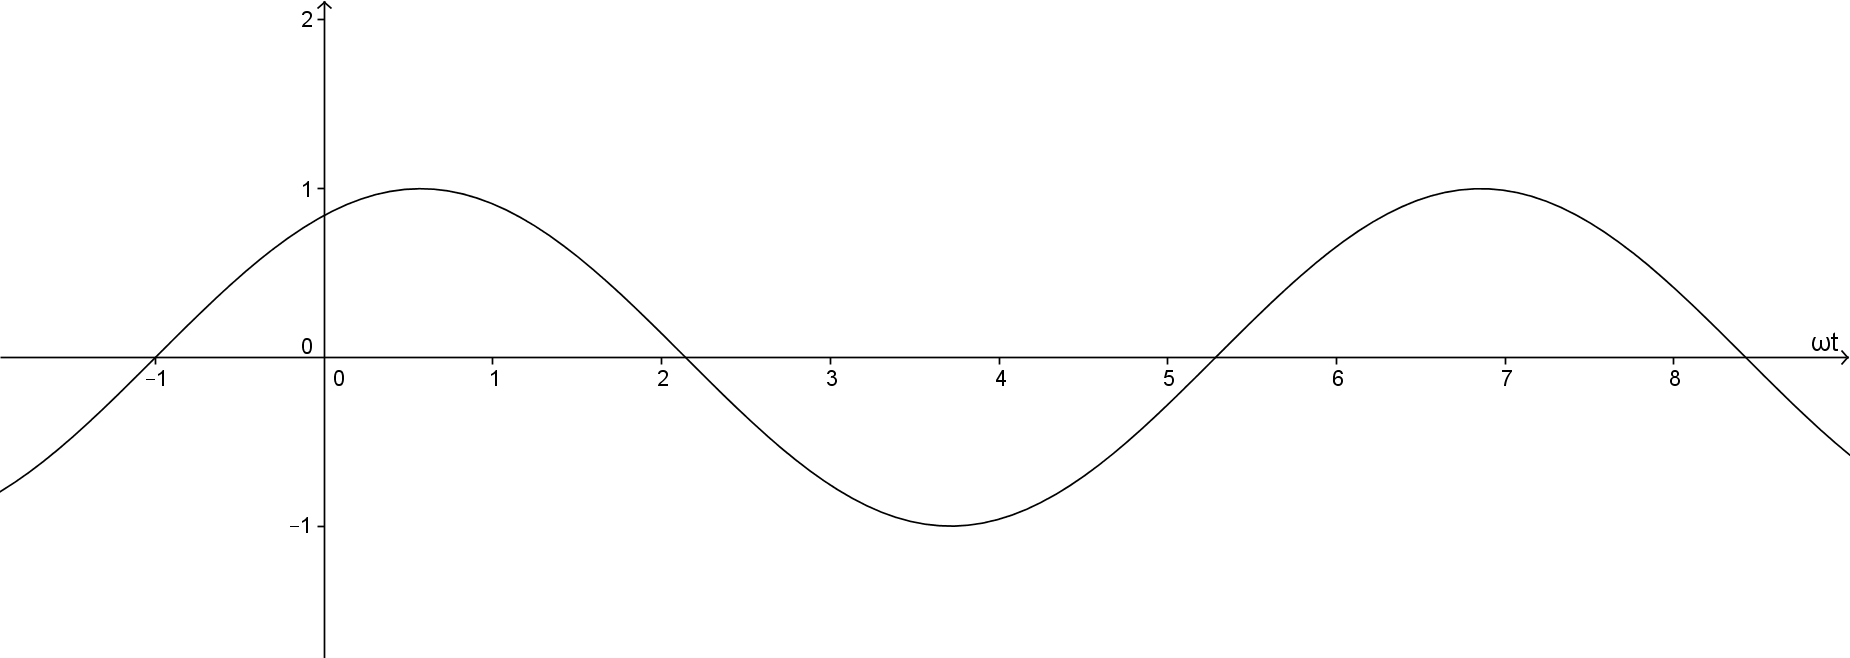
\includegraphics[width=\linewidth]{Bilder/39}
	\caption{}
	\vspace{-5em}
	$A(t)=A_0\sin(\omega t+\alpha_0)$\\
	$A_0$: Amplitude\\
	$\alpha_0$: Phase
\end{figure}

%bild 2
\begin{figure}[h!]
	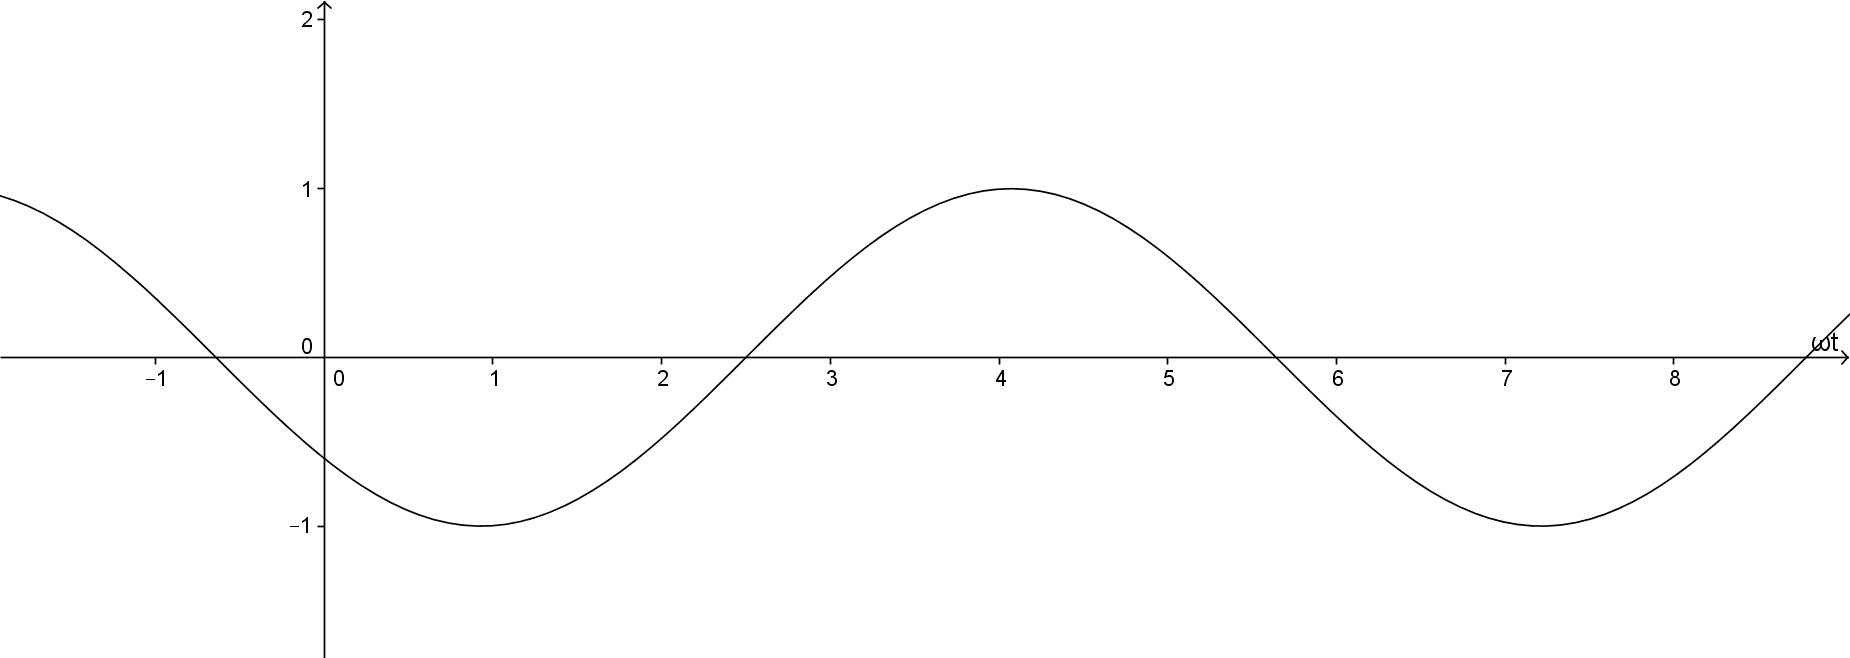
\includegraphics[width=\linewidth]{Bilder/40}
	\caption{}
	\vspace{-5em}
	$B(t)=B_0\sin(\omega t+\beta_0)$\\
	$B_0$: Amplitude\\
	$\beta_0$: Phase
\end{figure}

$\omega = \dfrac{2\pi}{T}$: Winkelgeschwindigkeit = Kreisfrequenz

\clearpage
\subsection{Überlagerung (=Superposition) der beiden Schwingungen}

\qquad$C(t) = A(t) + B(t)$

$C(t)$ ist wieder von der Form $C(t)=C_0\sin(\omega t + \gamma_0)$. Wie können $C_0$ und $\gamma_0$ bestimmt werden?

Schreibe $A(t)$ und $B(t)$ als Imaginärteile von \ul{komplexen} Schwingungen (rotierende Vektoren/Zeiger).

%bild 3
\imgw{Bilder/41}{}{}{10cm}

\clearpage
\subsection{A als Zeiger}
\redbox{$\ul{A}(t) = \ul{A}_0e^{\i\omega t}$} \hfill komplexe Schwingung mit komplexer Amplitude $\ul{A}_0$

%xxxxxxxxxxxxxxxxxxxxxxxxxxxxxxxxxxxxxxxxxxxxx

$\ul{A}(t)=\ul{A}_0e^{\i\omega t}=A_0e^{\i\alpha_0}e^{\i\omega t}\\
\Rightarrow A_0e^{\i(\omega t+\alpha_0)}$


$\ul{A}(t) = A_0(\cos(\omega t + \alpha_0)+\i\sin(\omega t + \alpha_0))= A_0\cos(\omega t + \alpha_0)+\i \underbrace{A_0\sin(\omega t + \alpha_0)}_{A(t)})$

$\underbrace{A(t)}_\text{reelle Schwingung} = \Im(\underbrace{\ul{A}(t)}_\text{komplexe Schwingung})$

%xxxxxxxxxxxxxxxxxxxxxxxxxxxxxxxxxxxxxxxxxxxxx

$|\ul{A}_0|=A_0$ (reelle Amplitude)

$\Arg(\ul{A}_0)=\alpha_0$ (Phase)

$\Rightarrow$ \redbox{$\ul{A}_0 = A_0e^{\i\alpha_0}$}

$\ul{A}(t)$: Zeiger zum Zeitpunkt $t$

Zeiger, der Länge $A_0$ rotiert mit Winkelgeschwindigkeit $\omega$ gegen den Uhrzeigersinn.

\vspace{-1.5cm}
\begin{align*}
A(t) = A_0\sin(\omega t+\alpha_0) &\longrightarrow \ul{A}(t) = A_0e^{\i(\omega t +\alpha_0)}\\
A(t) = \Im(\ul{A}(t)) &\longleftarrow \ul{A}(t)
\end{align*}

\subsection{B als Zeiger}
\vspace{-1.2cm}
\begin{minipage}{4cm}
	\begin{align*}
	\ul{B}(t) &= \ul{B}_0e^{\i\omega t}\\
	\ul{B}_0 &= B_0e^{\i\beta_0}\\
	B(t) &= \Im(\ul{B}(t))
	\end{align*}
\end{minipage}

\clearpage
\subsection{Überlagerung (Superposition)}
\vspace{-1.2cm}
\begin{minipage}{5.8cm}
	\begin{align*}
	C(t) &= A(t)+B(t)\\
	&= \Im(\ul{A}(t))+\Im(\ul{B}(t))\\
	&=\Im(\underbrace{\ul{A}(t)+\ul{B}(t)}_{\ul{C}(t)})\\
	&=\Im(\ul{C}(t))
	\end{align*}
\end{minipage}

\vspace{1cm}
D.h. für die Superposition $C(t)$ gilt\\
\parbox{20pt}{\quad}$C(t) = \Im(\ul{C}(t))$\\
mit\vspace{-1.5em}\\
\begin{minipage}{5.5cm}
	\begin{align*}
	\ul{C}(t) &= \ul{A}(t)+\ul{B}(t)\\
	&= \ul{A}_0e^{\i\omega t}+\ul{B}_0e^{\i\omega t}\\
	&= (\ul{A}_0+\ul{B}_0)e^{\i\omega t}
	\end{align*}
\end{minipage}\\
\parbox{17pt}{\quad}\redbox{$\ul{C}(t)=\ul{C}_0e^{\i\omega t}$}\\
wobei \redbox{$\ul{C}_0 = \ul{A}_0+\ul{B}_0$} (Addition der komplexen Amplituden).

$\Rightarrow$ reelle Superposition $C(t) = C_0\sin(\omega t+\gamma_0)$ mit $C_0 = |\ul{C}_0|$ und $\gamma_0 = \Arg(\ul{C}_0)$.

Addition der komplexen Amplituden

%bild 4 (Parallelogrammregel)
\imgw{Bilder/42}{Parallelogrammregel}{}{6cm}

\clearpage
\subsection{Zusammenfassung}
\ul{Geg:} $A(t)= A_0\sin(\omega t + \alpha_0), B(t) = B_0\sin(\omega t + \beta_0)$\\
(+ evtl. weitere Schwingungen $\rightarrow$ analoge Vorgehensweise)

\ul{Ges:} $C_0, \gamma_0$, sodass $A(t)+B(t) = C(t)= C_0\sin(\omega t+\gamma_0)$ gilt ($C_0 =$ Amplitude, $\gamma_0 = $ Phase der Überlagerung)

\begin{enumerate}[1.\text{ Schritt:}]
	\item komplexe Darstellung der Schwingungen\\
	$\ul{A}(t)= \ul{A}_0e^{\i\omega t}, \ul{B}(t)= \ul{B}_0e^{\i\omega t}$\\
	mit komplexen Amplituden $\ul{A}_0= A_0e^{\i\alpha_0},\ul{A}_0= A_0e^{\i\beta_0}$
	
	\item Addiere die komplexen Amplituden\\
	$\ul{C}_0 = \ul{A}_0 + \ul{B}_0$ ($\rightarrow$ Rechne $\ul{A}_0$ und $\ul{B}_0$ zunächst in kartesische Form um) und schreibe $\ul{C}_0$ in Exponentialform\\
	$\ul{C}_0 = C_0e^{\i\gamma_0}$, d.h. berechne $C_0 = |\ul{C}_0|$ und $\gamma_0 = \Arg(\ul{C}_0)$
	
	\item Reelle Beschreibung der Superposition\\
	$C(t) = C_0\sin(\omega t + \gamma_0)$\\
	(Hinweis: Bei mehr als zwei Schwingungen müssen entsprechend mehrere komplexe Amplituden addiert werden.)
\end{enumerate}

\clearpage
\chapter{Logik}
\section{Aussagen}

\Def Eine \ul{Aussage} ist ein sprachliches Gebilde, welches entweder wahr (w) oder falsch (f) ist. Aussagen werden mit großen Buchstaben $A, B, C, \ldots$ bezeichnet.

\Bsps
\begin{enumerate}
	\item 5 ist größer als 3 (w)
	\item 3 ist Teiler von 10 (f)
	\item DEG liegt in Niederbayern (w)
	\item Jede gerade Zahl größer als 2 ist eine Summe aus zwei Primzahlen (Goldbachsche Vermutung)
	
	($\rightarrow$ wahr oder falsch, jedoch weiß man es bis heute nicht, daher {\flqq Vermutung\frqq})
	
	\item $x^2+y^2=z^2$\hfill Fermat'sche {\flqq Vermutung\frqq}\\
	bewiesen durch Andrew Wiles
	
	\item Poincare-Vermutung\\
	bewiesen durch Perelman
	
	\item P-NP Problem
	noch nicht bewiesen
\end{enumerate}

\clearpage
\section{Verknüpfung von Aussagen, Aussagenlogik}

Sind $A$ und $B$ Aussagen, so definiert man wie folgt neue Aussagen:
\begin{enumerate}
	\begin{minipage}{\linewidth}
		{\bf\item Konjunktion} $A\land B$ ({\flqq $A$ und $B$\frqq})
		
		$A\land B$ ist genau wahr, wenn $A$ und $B$ wahr sind.
		
		Wahrheitstabelle:
		\begin{tabular}{c|c|c}
			$A$ & $B$ & $A\land B$ \\
			\hline w & w & w \\
			w & f & f \\
			f & w & f \\
			f & f & f
		\end{tabular}
	\end{minipage}
	
	\begin{minipage}{\linewidth}
		{\bf\item Disjunktion} $A\lor B$ ({\flqq $A$ oder $B$\frqq}) {\flqq inklusives oder\frqq}
		
		$A\lor B$ ist genau dann wahr, wenn $A$ oder $B$ wahr ist (d.h. mindestens eine der beiden Aussagen wahr ist)
		
		Wahrheitstabelle:
		\begin{tabular}{c|c|c}
			$A$ & $B$ & $A\lor B$ \\
			\hline w & w & w \\
			w & f & w \\
			f & w & w \\
			f & f & f
		\end{tabular}
	\end{minipage}
	
	\begin{minipage}{\linewidth}
		{\bf\item Negation} $\neg A$ ({\flqq nicht $A$\frqq})
		
		$\neg A$ ist genau dann wahr, wenn $A$ falsch ist
		
		Wahrheitstabelle:
		\begin{tabular}{c|c}
			$A$ & $\neg A$ \\
			\hline w & f \\
			f & w
		\end{tabular}
	\end{minipage}
	
	\begin{minipage}{\linewidth}
		{\bf\item Implikation} $A\imp B$ ({\flqq $A$ impliziert $B$\frqq}, {\flqq aus $A$ folgt $B$\frqq})
		
		Wahrheitstabelle:
		\begin{tabular}{c|c|c}
			$A$ & $B$ & $A\imp B$ \\
			\hline w & w & w \\
			w & f & f \\
			f & w & w \\
			f & f & w
		\end{tabular}
	\end{minipage}
	
	\begin{minipage}{\linewidth}
		{\bf\item Äquivalenz} $A\eq B$ ({\flqq $A$ äquivalent $B$\frqq}, {\flqq aus $A$ folgt $B$ und aus $B$ folgt $A$\frqq})
		
		$A\eq B$ ist genau dann wahr, wenn $A$ und $B$ denselben Wahrheitswert besitzen.
		
		Wahrheitstabelle:
		\begin{tabular}{c|c|c}
			$A$ & $B$ & $A\eq B$ \\
			\hline w & w & w \\
			w & f & f \\
			f & w & f \\
			f & f & w
		\end{tabular}
	\end{minipage}
\end{enumerate}

\Bem\quad\\
$\neg$ bindet stärker als $\land, \lor, \imp, \eq$\\
$\land, \lor$ binden stärker als $\imp, \eq$

\Def
\begin{enumerate}[a)]
	\item Aus Aussagen $A,B,C,\ldots$ und dessen Verknüpfungen $\land, \lor, \neg, \imp, \eq$ können beliebige, neue Aussagen gebildet werden. Betrachtet man $A,B,C,\ldots$ als Variablen (oder Platzhalter) für Aussagen, so spricht man \ul{Formeln für Aussagen} oder \ul{Aussagenformeln} oder \ul{aussagenlogische Formel}.
	
	\item Zwei Aussageformeln $P$ und $Q$ heißen \ul{äquivalent}, i.Z. $P\equiv Q$ (bzw. $P\eq Q$) wenn sie für \ul{jede Belegung} ihrer Variablen mit wahren oder falschen Aussagen übereinstimmende Wahrheitswerte besitzen.
	
	\item Eine Aussageformel $P$ heißt \ul{Tautologie} bzw. \ul{Kontradiktion} wenn sie für \ul{jede} Belegung ihrer Variablen mit wahren oder falschen Aussagen, stets den Wahrheitswert w (bzw. f) liefert.
\end{enumerate}

\Bsps
\begin{enumerate}
	\item $\neg(A\lor B) \equiv \neg A \land \neg B$
	
	\begin{tabular}{c|c|c|c}
		$A$ & $B$ & $A\lor B$ & $\neg(A\lor B)$ \\ 
		\hline 
		w & w & w & f \\ 
		w & f & w & f \\ 
		f & w & w & f \\ 
		f & f & f & w 
	\end{tabular} 
	
	\begin{tabular}{c|c|c|c|c}
		$A$ & $B$ & $\neg A$ & $\neg B$ & $\neg A \land \neg B$ \\ 
		\hline 
		w & w & f & f & f \\ 
		w & f & f & w & f \\ 
		f & w & w & f & f \\ 
		f & f & w & w & w 
	\end{tabular} 
	
	\item $A \lor \neg A$
	
	\begin{tabular}{c|c|c}
		$A$ & $\neg A$ & $A \lor \neg A$ \\ 
		\hline 
		w & f & w \\ 
		f & w & w
	\end{tabular}
	
	$\Rightarrow A \lor \neg A$  ist eine Tautologie
	
	\item $A \land \neg A$
	
	\begin{tabular}{c|c|c}
		$A$ & $\neg A$ & $A \land \neg A$ \\ 
		\hline 
		w & f & f \\ 
		f & w & f
	\end{tabular}
	
	$\Rightarrow A \land \neg A$  ist eine Kontradiktion
	
	\item $A\imp B \equiv \neg(A\land \neg B) \equiv \neg A \lor B$
	
	\begin{tabular}{c|c|c|c|c}
		$A$ & $B$ & $A\imp B$ & $\neg(A\land \neg B)$ & $\neg A \lor B$ \\ 
		\hline 
		w & w & w & w & w \\ 
		w & f & f & f & f \\ 
		f & w & w & w & w \\ 
		f & f & w & w & w \\
	\end{tabular} 
\end{enumerate}

\Satz{Für Aussagenvariablen $A,B,C$ gilt:
	
	\qquad$F$ = Kontradiktion
	
	\qquad$W$ = Tautologie}

\begin{enumerate}
	\item $A \land B \equiv B \land A$\\
	$A \lor B \equiv B \lor A$
	\hfill{Kommutativität}
	\item $A \land (B \land C) \equiv (A \land B) \land C$\\
	$A \lor (B \lor C) \equiv (A \lor B) \lor C$
	\hfill{Assoziativität}
	\item $A \land (B \lor C) \equiv (A \land B) \lor (A \land C)$\\
	$A \lor (B \land C) \equiv (A \lor B) \land (A \lor C)$
	\hfill{Distributivität}
	\item $A\land (A\lor B) \equiv A$\\
	$A\lor (A\land B) \equiv A$
	\hfill{Absorption}
	\item $A\land A \equiv A$\\
	$A\lor A \equiv A$
	\hfill{Idempotenz}
	\item $\neg(\neg A) \equiv A$
	\item $\neg(A\land B) \equiv \neg A \lor \neg B$\\
	$\neg(A\lor B) \equiv \neg A \land \neg B$
	\hfill{Gesetze von de Morgan}
	\item $A \lor F \equiv A, \qquad A\land W \equiv A$
	\item $A \land \neg A \equiv F, \qquad A\lor \neg A \equiv W$
	\item $A\land F \equiv F, \qquad A\lor W \equiv W$
	\item $A\imp B \equiv \neg A \lor B$\\
	$A\imp B \equiv \neg B \imp \neg A$\\
	$A\eq B \equiv (A\imp B) \land (B\imp A) \equiv (\neg A \lor B) \land (\neg B \lor A)$\\
	$A\eq B \equiv \neg A \eq \neg B$
\end{enumerate}

\Bsp Zeigen Sie, dass die Aussageformeln $A\imp (B\imp\neg C)$ und $\neg(A\land B\land C)$ äquivalent sind durch \\
a) Umformungen (Äquivalenzumformungen) \\
b) Erstellen einer Wertetabelle

zu a) 
\begin{align*}
A\imp (B\imp\neg C) &\equiv \neg A\lor (\neg B\lor\neg C)\\
&\equiv \neg (A\land \neg(\neg B\lor\neg C))\\
&\equiv \neg (A\land (B\land C))\\
&\equiv \neg (A\land B\land C)
\end{align*}

zu b)

\begin{tabular}{c|c|c|c|c|c}
	$A$ & $B$ & $C$ & $\neg (A\land B\land C)$ & $B\imp\neg C$ & $A\imp (B\imp\neg C)$ \\ 
	\hline 
	w & w & w & f & f & f \\ 
	w & w & f & w & w & w \\ 
	w & f & w & w & w & w \\ 
	w & f & f & w & w & w \\ 
	f & w & w & w & f & w \\ 
	f & w & f & w & w & w \\ 
	f & f & w & w & w & w \\ 
	f & f & f & w & w & w \\ 
\end{tabular} 

\clearpage
\subsection{Schaltalgebra}
Der Erfolg der modernen Digitaltechnik gründet auf der Möglichkeit
\begin{itemize}
	\item Informationen in Einheiten von {\flqq Bits\frqq} (der kleinsten digitalen Informationseinheit) darzustellen bzw. zu speichern
	\item Informationen durch logische Verknüpfungen zu verarbeiten
\end{itemize}

Die der Schaltalbebra zugrunde liegende (Schalt-)Logik ist zur Aussagelogik (bzw. Boolschen Algebra) äquivalent. Man verwendet analoge Formeln , jedoch anstatt der Aussagevariablen $A,B,C,\ldots$ nun Variablen $x_1,x_2,x_3,\ldots$ (mit Werten 0 oder 1), welche die (digitalen) Eingänge der logischen Schaltungen repräsentieren.

Jede logische Formel hat eine entsprechende Darstellung im Schaltplan.

\clearpage
Für die atomaren Formeln $x_1\land x_2, x_1\lor x_2, \neg x_1$ gilt

\begin{longtable}{c|c|c|c}
	Bezeichnung & logische & Symbol im Schaltbild (IEC) & Wahrheitstabelle \\ 
	\hline 
	UND(AND)-Gatter & $x_1\land x_2$ & 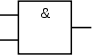
\includegraphics[height=1.4cm]{Bilder/43} & \begin{tabular}{c|c|c}
		$x_1$ & $x_2$ & $x_1\land x_2$ \\ 
		\hline 
		1 & 1 & 1 \\ 
		1 & 0 & 0 \\ 
		0 & 1 & 0 \\ 
		0 & 0 & 0 \\ 
	\end{tabular}  \\ 
	\hline 
	ODER(OR)-Gatter & $x_1\lor x_2$ & 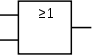
\includegraphics[height=1.4cm]{Bilder/44} & \begin{tabular}{c|c|c}
		$x_1$ & $x_2$ & $x_1\lor x_2$ \\ 
		\hline 
		1 & 1 & 1 \\ 
		1 & 0 & 1 \\ 
		0 & 1 & 1 \\ 
		0 & 0 & 0 \\ 
	\end{tabular}  \\ 
	\hline 
	NICHT(NOT)-Gatter & $\neg x_1$ & 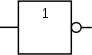
\includegraphics[height=1.4cm]{Bilder/45} & \begin{tabular}{c|c}
		$x_1$ & $\neg x_1$ \\ 
		\hline 
		1 & 0 \\ 
		0 & 1 \\ 
	\end{tabular}  \\ 
	\hline
\end{longtable} 

\clearpage
Man unterscheidet noch weitere Gatter

\begin{longtable}{c|c|c|c}
	Bezeichnung & logische & Symbol im Schaltbild (IEC) & Wahrheitstabelle \\ 
	\hline 
	NAND-Gatter & $\neg(x_1\land x_2)$ & 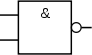
\includegraphics[height=1.4cm]{Bilder/46} & \begin{tabular}{c|c|c}
		$x_1$ & $x_2$ & $\neg(x_1\land x_2)$ \\ 
		\hline 
		1 & 1 & 0 \\ 
		1 & 0 & 1 \\ 
		0 & 1 & 1 \\ 
		0 & 0 & 1 \\ 
	\end{tabular}  \\ 
	\hline 
	NOR-Gatter & $\neg(x_1\lor x_2)$ & 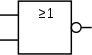
\includegraphics[height=1.4cm]{Bilder/47} & \begin{tabular}{c|c|c}
		$x_1$ & $x_2$ & $\neg(x_1\lor x_2)$ \\ 
		\hline 
		1 & 1 & 0 \\ 
		1 & 0 & 0 \\ 
		0 & 1 & 0 \\ 
		0 & 0 & 1 \\ 
	\end{tabular}  \\ 
	\hline 
	XOR-Gatter & \parbox{2.7cm}{$x_1\lxor x_2 \\\equiv (x_1\land\neg x_2)\lor (\neg x_1\land x_2)$} & 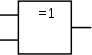
\includegraphics[height=1.4cm]{Bilder/48} & \begin{tabular}{c|c|c}
		$x_1$ & $x_2$ & $x_1\lxor x_2$ \\ 
		\hline 
		1 & 1 & 0 \\ 
		1 & 0 & 1 \\ 
		0 & 1 & 1 \\ 
		0 & 0 & 0 \\ 
	\end{tabular}  \\ 
	\hline 
	XNOR-Gatter & $\neg(x_1\lxor x_2)$ & 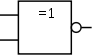
\includegraphics[height=1.4cm]{Bilder/49} & \begin{tabular}{c|c|c}
		$x_1$ & $x_2$ & $\neg(x_1\lxor x_2)$ \\ 
		\hline 
		1 & 1 & 1 \\ 
		1 & 0 & 0 \\ 
		0 & 1 & 0 \\ 
		0 & 0 & 1 \\ 
	\end{tabular}  \\ 
	\hline 
\end{longtable} 

\clearpage
\Bsps
\begin{enumerate}
	\item Zeichnen Sie das zugehörige Schaltbild
	\begin{enumerate}
		\item $\neg x_1\land x_2$
		\imgw{Bilder/50}{}{}{3cm}
		
		\item $(x_1\lor\neg x_2)\land x_3$
		\imgw{Bilder/51}{}{}{5cm}
		
		\item $(\neg x_1\lxor x_2)\lor\neg(x_1\land x_2)$
		\imgw{Bilder/52}{}{}{6cm}
	\end{enumerate}
	
	\item Bestimmen Sie die zugehörigen logische Formel
	\begin{enumerate}
		\item $(x_1\land x_2)\lxor(\neg x_1\lor\neg x_2)$
		\imgw{Bilder/53}{}{}{5.5cm}
		
		\item $((x_1\lxor x_2)\lor \neg x_3)\land x_1$
		\imgw{Bilder/54}{}{}{6cm}
		
		\item $C=x_1\land x_2$\\
		$S=x_1\lxor x_2 = (x_1\land\neg x_2)\lor(\neg x_1 \land x_2)$
		\imgw{Bilder/55}{Halbaddierer}{}{6cm}
		\imgw{Bilder/56}{}{}{5cm}
	\end{enumerate}
\end{enumerate}

\clearpage
\subsection{Boolesche Funkion/Schaltfunktion}
\Def Unter einer Booleschen Funktion (Schaltfunktion) versteht man eine (beliebige) Funktion\\
$f:\{0;1\}^n\to\{0;1\}^m, (x_1,\ldots,x_n)\mapsto(y_1,\ldots,y_m)$

$f(x_1,\ldots,x_n)=(\underbrace{f_1(x_1,\ldots,x_n)}_{y_1},\underbrace{f_2(x_1,\ldots,x_n)}_{y_2},\ldots,\underbrace{f_m(x_1,\ldots,x_n)}_{y_m})$

$f_j(x_1,\ldots,x_n)\in\{0;1\}\qquad(j=1,\ldots,m)$

%bild 8
\imgw{Bilder/57}{}{}{7cm}

Jede logische Formel $\varphi(x_1,\ldots,x_n)$ in den Variablen $x_1,\ldots,x_n$ definiert eine Boolesche Funktion\\
$f_\varphi:\{0;1\}^n\to\{0;1\}, (x_1,\ldots,x_n)\mapsto \left\{ \begin{array}{ll}
	0, &\text{falls }\varphi(x_1,\ldots,x_n)\text{ falsch}\\
	1, &\text{falls }\varphi(x_1,\ldots,x_n)\text{ wahr}\\
	\end{array}\right. $
	
%bild 9
\imgw{Bilder/58}{}{}{4.5cm}

\Bsp
$\varphi = x_1\lor x_2$

$f_\varphi :\{0,1\}^2\to\{0,1\},(x_1,x_2)\mapsto x_1\lor x_2 = y$

\Bsp
$\varphi = x_1\land x_2$

$f_\varphi :\{0,1\}^2\to\{0,1\},(x_1,x_2)\mapsto x_1\land x_2 = y$

\Satz{{\bf Hauptsatz der Schaltalgebra:}\\
	\\
	\ul{Jede} Boolesche Funktion $f :\{0,1\}^n\to\{0,1\}$ lässt sich durch eine Formel $\varphi(x_1,\ldots,x_n)$, die durch die drei logischen Operatoren UND, ODER, NEG gegeben ist, darstellen.\\
	Man bezeichnet deshalb die logischen Operatoren UND, ODER, NEG als \ul{vollständiges Logiksystem} (\ul{Basissystem}).}

Weitere vollständige Logiksysteme (Basissysteme)
\begin{enumerate}
	\item $\land$ UND, $\neg$ NEG\\
	$x_1\lor x_2\equiv \neg(\neg x_1\land \neg x_2)$
	
	\item $\lor$ ODER, $\neg$ NEG\\
	$x_1\land x_2\equiv \neg(\neg x_1\lor \neg x_2)$
	
	\item NAND
	%bild 1
	\begin{figure}[h!]
		\begin{minipage}{0.32\linewidth}
			\centering 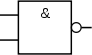
\includegraphics[height=1.4cm]{Bilder/46}
			\caption{NAND}
		\end{minipage}
		\begin{minipage}{0.32\linewidth}
			\centering 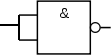
\includegraphics[height=1.4cm]{Bilder/72}
			\caption{NEG}
		\end{minipage}
		\begin{minipage}{0.32\linewidth}
			\centering 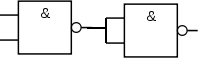
\includegraphics[height=1.5cm]{Bilder/73}
			\caption{AND}
		\end{minipage}
	\end{figure}

	\item NOR
	%bild 2
	\begin{figure}[h!]
		\begin{minipage}{0.32\linewidth}
			\centering 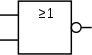
\includegraphics[height=1.4cm]{Bilder/47}
			\caption{NOR}
		\end{minipage}
		\begin{minipage}{0.32\linewidth}
			\centering 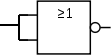
\includegraphics[height=1.4cm]{Bilder/75}
			\caption{NEG}
		\end{minipage}
		\begin{minipage}{0.32\linewidth}
			\centering 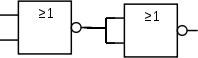
\includegraphics[height=1.5cm]{Bilder/74}
			\caption{OR}
		\end{minipage}
	\end{figure}
\end{enumerate}

\clearpage
\section{Formeln über R bzw. C, Quantoren}
Wir betrachten \ul{Terme} und \ul{Formeln} über den reellen bzw. komplexen Zahlen ($\R$ bzw. $\C$). Terme und Formeln sind Gegenstand einer sogenannten \ul{formalen Sprache}.\hfill\gray{Bison, Yacc}

Zunächst definiert man das \ul{Alphabet} der formalen Sprache:\\
es besteht aus
\begin{enumerate}
	\item Zeichen für Variablen $x_1,x_2,x_3,\ldots$ (über den komplexen Zahlen verwenden wir $z_1,z_2,\ldots$)
	\item Zeichen für Konstanten $c$ ($c\in\R$ bzw. $c\in\C$)
	\item Zeichen für Addition, Multiplikation, Division $+,\cdot,-,:$ (bzw. $\dfrac{\square}{\square}$)
	\item logische Zeichen $\neg, \land,\lor,\imp,\eq$
	\item Relations- bzw. Funktionszeichen $=,\le,\ge,<,> (\text{bei }\R), f(\text{z.B. }\sin, \cos,\ldots)$
	\item Quantoren\\
	$\forall$ (für alle) All-Quantor\\
	$\exists$ (es existiert) Existenz-Quantor
	\item Hilfszeichen (,),[,],\{,\}
\end{enumerate}

\Def\quad\\
\Graybox{{\bf (Term) induktive Definition}
\begin{enumerate}
	\item Variablen und Konstanten sind Terme (atomare Terme, Induktionsanfang)
	\item Sind $T_1$ und $T_2$ Terme, so sind auch\\
	$T_1+T_2,T_1-T_2,T_1\cdot T_2,T_1:T_2,\dfrac{T_1}{T_2} \text{ und } (T),[T],\{T\}$\\
	Terme (Induktionsschritt)
	\item Sind $T_1, \ldots, T_r$ Terme und ist $f$ ein r-stelliges Funktionszeichen, so ist auch $f(T_1, \ldots, T_r)$ ein Term.
	\item Keine weiteren Zeichenketten sind Terme.
\end{enumerate}}

\Def\quad\\
\Graybox{{\bf (Formel) induktive Definition}
	\begin{enumerate}
		\item Sind $T_1$ und $T_2$ Terme, so ist $T_1=T_2$ eine Formel (bei Formeln über $\R$ sind auch $T_1\le T_2,T_1\ge T_2,T_1<T_2,T_1>T_2$ Formeln)\\
		(Induktionsanfang, atomare Formeln)
		\item Sind $\varphi,\psi$ Formeln, so sind auch $\neg\varphi$ (bzw. $\ol{\varphi}$), $(\varphi),[\varphi],\{\varphi\}, \varphi\land\psi,\varphi\lor\psi,\varphi\imp\psi,\varphi\eq\psi\text{ und }\forall x\varphi, \exists x\varphi$ Formeln
		\item Keine weiteren Zeichenketten sind Formeln
	\end{enumerate}}

\Def\quad\\
\Graybox{{\bf (Quantoren)}\\
\\
Die Symbole $\forall$ und $\exists$ heißen \ul{Quanotoren}; speziell heißt $\forall$ \ul{All-Quantor} und $\exists$ heißt \ul{Existenzquantor}.

Ist $x$ eine Variable, so bedeutet $\forall x$ {\flqq für alle $x$\frqq}\\
$\exists x$ {\flqq es existiert (gibt) ein $x$\frqq}

In den Formeln $\forall x\varphi$ und $\exists x\varphi$ liegt die Variable $x$ im Wirkungsbereich eines Quantors und wird als \ul{gebundene} Variable der Formel bezeichnet; ansonsten heißt die Variable \ul{frei} (für die Formel).}

\Bsp für Terme

$x_1\cdot x_2 - 1,\quad x_1^2+\sqrt{2},\quad 2x_1^2+4x_1+9,\quad \dfrac{x_1}{x_1^2+1}$\quad (in $\R$)

speziell in $\C$: $z_1^3-5\i$ (Konstante $i\in\C$)

\Bsp für Formeln

$2x_1-3 = 1;\quad x_1^2+x_2^2<1;\quad\dfrac{1}{x_1^2+1}<x_2^2$\\
$z_1\cdot \ol{z_2} < 4;\quad (5x_1+6x_2=1)\land(x_1^2+x_2^2=1)$\\
$\neg(4x_1+3x_2>5);\\
\forall x_1\quad x_1\ge 0\quad (x_1 \text{ gebundene Variable})$\\
$\exists x_1\quad 5x_1^2+2x_2^2=1\quad (x_1\text{ gebunden, }x_2\text{ frei})$

\Def
\begin{enumerate}
	\item Sind die freien Variablen einer Formel $\varphi$ in der Menge $\{x_1,\ldots, x_n\}$ enthalten, so schreibt man auch $\varphi(x_1,\ldots, x_n)$ statt $\varphi$.
	\item Für eine Formel $\varphi(x_1,\ldots, x_n)$ bzw. $\varphi(z_1,\ldots, z_n)$ definiert man die \ul{Erfüllungsmenge} durch $M_\varphi = \{(a_1,\ldots, a_n)\in\R^n\mid\varphi(a_1,\ldots, a_n)\text{ ist in }\R\text{ wahr}\}$ (falls $\varphi$ eine Formel über $\R$ ist)
	
	$M_\varphi = \{(a_1,\ldots, a_n)\in\C^n\mid\varphi(a_1,\ldots, a_n)\text{ ist in }\C\text{ wahr}\}$ (falls $\varphi$ eine Formel über $\C$ ist)
\end{enumerate}

\Bem Besitzt eine Formel \ul{keine freien} Variablen, so stellt sie eine Aussage dar, die in $\R$ (bzw. $\C$) wahr oder falsch ist.

\clearpage
\Bsp Erfüllungsmengen für Formeln über $\R$, Aussagen über $\R$
\begin{enumerate}
	\item $\varphi(x_1):=(x_1\ge 0)$\qquad ($x_1\in\R$, d.h. $\varphi$ ist eine Formel über $\R$)\\
	$x_1$ freie Variable
	
	$M_\varphi = \{a_1\in\R\mid a_1\ge 0\text{ ist wahr in }\R\} = \Rop$
	
	\item $\varphi(x_1):=(4x_1-2 = 0)\qquad(x_1\in\R)$\\
	$x_1$ freie Variable
	
	$M_\varphi = \{\frac{1}{2}\}$
	
	\item $\varphi(x_1, x_2):=((2x_1-x_2=4)\land(-x_1+x_2=2))$\\
	$x_1,x_2$ freie Variablen
	
	\begin{align*}
	2x_1-x_2&=4 &\text{(I)}\\
	-x_1+x_2&=2 &\text{(II)}\\
	\hline
	x_1 &= 6 &\text{(I)+(II)}\\
	x_2 &= 2+x_1 = 8 &\text{in (II)}
	\end{align*}
	
	$M_\varphi = \{(6,8)\}$
	
	\item $\varphi(x_1, x_2):=((2x_1-x_2<4)\land(-x_1+x_2<2))$\\
	$x_1,x_2$ freie Variablen
	
	\begin{align*}
	2x_1-x_2&<4 &\text{(I)}\\
	-x_1+x_2&<2 &\text{(II)}\\
	\hline
	2x_1-4 &< x_2 &\text{(I)}\\
	x_2 &< x_1 + 2 &\text{(II)}\\
	\hline
	2x_1-4 &< x_2 < x_1 + 2
	\end{align*}
	
	$M_\varphi = $ siehe Zeichnung
	
	\begin{minipage}{\linewidth}
	\definecolor{qqccqq}{rgb}{0.,0.8,0.}
	\begin{tikzpicture}[line cap=round,line join=round,>=triangle 45,x=1.0cm,y=1.0cm]
	\draw[->,color=black] (-2.5,0.) -- (6.5,0.);
	\foreach \x in {-2.,-1.,1.,2.,3.,4.,5.,6.}
	\draw[shift={(\x,0)},color=black] (0pt,2pt) -- (0pt,-2pt) node[below] {\footnotesize $\x$};
	\draw[->,color=black] (0.,-1.7) -- (0.,9.5);
	\foreach \y in {-1.,1.,2.,3.,4.,5.,6.,7.,8.,9.}
	\draw[shift={(0,\y)},color=black] (2pt,0pt) -- (-2pt,0pt) node[left] {\footnotesize $\y$};
	\draw[color=black] (0pt,-10pt) node[right] {\footnotesize $0$};
	\clip(-2.5,-1.7) rectangle (6.5,9.5);
	\draw[dash pattern=on 1pt off 1pt,color=qqccqq,fill=qqccqq,fill opacity=0.2](6.00000063875,8.0000006836)--(-2.17382861777,-0.173828572918)--(-2.17382861777,-1.7)--(1.13945099284,-1.7)--(6.00000063875,8.0000006836);
	\draw[dash pattern=on 1pt off 1pt,color=qqccqq,fill=qqccqq,fill opacity=0.2](6.00000063875,8.0000006836)--(-2.17382861777,-0.173828572918)--(-2.17382861777,-1.7)--(1.13945099284,-1.7)--(6.00000063875,8.0000006836);
	\end{tikzpicture}
	\end{minipage}

	\item $\varphi(x_1):=\exists x_2\quad ((2x_1-x_2<4)\land(-x_1+x_2<2))$\\
	$x_1$ frei, $x_2$ gebunden
	
	$M_\varphi = \{x_1\in\R\mid x_1<6\} = ]-\infty;6[$
	
	\begin{minipage}{\linewidth}
	\item $\exists x_1\forall x_2\qquad x_1 = x_2^2$ \qquad (f) (über $\R$)
	\item $\forall x_1\exists x_2\qquad x_1 = x_2^2$ \qquad (f) (über $\R$)\\
	\gray{$\forall x_1\exists x_2\qquad x_1\ge 0\imp x_1 = x_2^2$ \qquad (w) (über $\R$)}
	\item $\forall x_1\exists x_2\qquad x_2 = x_1^2$ \qquad (w) (über $\R$)
	\end{minipage}
\end{enumerate}

\clearpage
\Bsp Erfüllungsmengen für Formeln über $\C$, Aussagen über $\C$
\begin{enumerate}
	\item $\varphi(z_1):=(z_1^2+1=0)$
	
	$M_\varphi = \{\i,-\i\}$
	
	\item $\varphi(z_1):=(z_1^3+8e^{\i\frac{\pi}{4}}=0)$
	
	\begin{align*}
	z_1^3&=-8e^{\i\frac{\pi}{4}}\\
	-1&= e^{\i\pi}\\
	z_1^3&=8 e^{\i\pi}e^{\i\frac{\pi}{4}}\\
	z_1^3&=8 e^{\i\frac{5}{4}\pi}
	\end{align*}
	
	$M_\varphi=\{2e^{\i\frac{5}{12}\pi};2e^{\i\frac{13}{12}\pi};2e^{\i\frac{7}{4}\pi}\}$
	
	\item $\varphi(z_1):=(z_1\cdot \ol{z_1} = 4)$
	
	$M_\varphi=\{z_1\in\C\mid|z_1| = 2\}$
	
	\item $\varphi(z_1, z_2):=(z_1\cdot \ol{z_1} = z_2\cdot \ol{z_2})$
	
	$M_\varphi=\{(z_1,z_2)\in\C^2\mid|z_1| = |z_2|\}\\
	=\{(z_1,z_2)\in\C^2\mid\\ z_1\text{ und }z_2\text{ liegen auf dem selben Kreis mit Mittelpunkt }0\in\C\}$
	
	\begin{minipage}{\linewidth}
	\item $\exists z_1\forall z_2\qquad z_1=z_2^2$\qquad (f) (über $\C$)
	\item $\forall z_1\exists z_2\qquad z_1=z_2^2$\qquad (w) (über $\C$)
	\item $\forall z_1\exists z_2\qquad z_2=z_1^2$\qquad (w) (über $\C$)
	\end{minipage}
\end{enumerate}

\clearpage
\section{Vollständige Induktion}
Induktionsaxiom (5. Peano-Axiom)\\
Für eine Teilmenge $M\subseteq\N$ der natürlichen Zahlen gelte:\\
\begin{enumerate}
	\item $1\in M$
	\item $n\in M \imp n+1\in M$
\end{enumerate}
Dann folgt $M = \N$

\Bem Das Induktionsaxiom ist Bestandteil der Definition der natürlichen Zahlen (Peano-Axiome) und beschreibt eine bestimmte Eigenschaft der natürlichen Zahlen.

\subsection{Vollständige Induktion}

Wir betrachten eine (unendliche) Folge von Aussagen $A(n) (n\in\N)$ und möchten zeige, dass $A(n)$ für \ul{jedes} $n\in\N$ wahr ist.

Mittels vollständiger Induktion kann man dies in zwei Schritten zeigen:

\begin{enumerate}
	\item Induktionsanfang ($n=1$)\\
	Zeige, dass \redbox{$A(1)$ wahr ist}.
	\item Induktionsschritt ($n\imp n+1$)\\
	Unter der Annahme, dass $A(n)$ wahr ist (Induktionsannahme), zeige man, dass auch $A(n+1)$ wahr ist, d.h. zeige \redbox{$A(n)\imp A(n+1)$}
\end{enumerate}

Mithilfe des Induktionsaxioms der natürlichen Zahlen gilt dann\\
$M=\{n\in\N\mid A(n)\text{ ist wahr}\} = \N$\\
d.h. $A(n)$ ist für \ul{jedes} $n\in\N$ wahr.

\Bem Modifikation

\Greenbox{Aussagen $A(n), n\in\Z,n\ge n_0$

\begin{enumerate}
	\item Induktionsanfang: ($n=n_0$)\\
	Zeige, dass $A(n_0)$ wahr ist
	\item Induktionsschritt ($n\imp n+1$)\\
	Zeige: $A(n)\imp A(n+1)$
\end{enumerate}}

\Bsp Zeigen Sie mittels vollständiger Induktion:
\begin{enumerate}
	\item\label{a1} $\sum\limits_{k=0}^{n}k = \dfrac{n(n+1)}{2}$
	\item\label{a2} $\sum\limits_{k=0}^{2n-1}k = n^2$\\
	$k$ ungerade
	
	\item $\#k$-elementige Teilmengen einer $n$-elementige Menge ($k \le n$) ist gleich $\binom{n}{k}$
	
	\item Bemoullische Ungleichung\\
	$(1+x)^n \ge 1+nx$\qquad$(x\in\R, 1+x\ge 0, n\in\N)$
	
	\item Binomischer Lehrsatz\\
	$(a+b)^n = \sum\limits_{k=0}^{n}\binom{n}{k} a^{n-k}b^k$
\end{enumerate}
%HÜ

\paragraph{zu \ref*{a1})}

$A(n):=(\sum\limits_{k=0}^{n}k = \dfrac{n(n+1)}{2})\qquad (n= 0,1,2,\ldots)$

Induktionsanfang: ($n=0$)\\
Zeige, dass $A(0)$ wahr ist.

\begin{align*}
\sum\limits_{k=0}^{n}k &= 0\\
\dfrac{n(n+1)}{2} &= 0
\end{align*}

Induktionsschritt: ($n\imp n+1$)\\
Induktionsannahme $A(n)$ ist wahr, d.h. es gelte $\sum\limits_{k=0}^{n}k = \dfrac{n(n+1)}{2}$

zeige $A(n+1)$ ist wahr d.h.

\begin{align*}
\sum\limits_{k=0}^{n+1}k &\stackrel{!}{=} \dfrac{(n+1)(n+2)}{2}\\
\underbrace{\sum\limits_{k=0}^{n}k}_{\dfrac{n(n+1)}{2}} + (n+1) &= \dfrac{n(n+1)}{2} +(n+1)\\
&= \dfrac{n(n+1)+2(n+1)}{2}\\
&= \dfrac{(n+1)(n+2)}{2}
\end{align*}

\paragraph{zu \ref*{a2})}

$A(n):= ((1+x)^n\ge 1+nx)\qquad (n= 1,2,3,\ldots)$

Induktionsanfang: (n=1)\\
Zeige, dass $A(1)$ wahr ist.

\begin{align*}
(1+x)^1&= 1+x\\
1+1x&=1+x
\end{align*}

Induktionsschritt: ($n\imp n+1$)\\
Induktionsannahme: $A(n)$ ist wahr, d.h. $(1+x)^n \ge 1+nx$\\
Zeige, dass $A(n+1)$ wahr ist, d.h.

\begin{align*}
(1+x)^{n+1} &\stackrel{!}{\ge} 1+(n+1)x\\
(1+x)^{n+1} &=\underbrace{(1+x)^n}_{\ge 1+nx}(1+x)\\
\underbrace{(1+x)^n}_{\ge 1+nx}(1+x)&\ge (1+nx)(1+x)\\
(1+x)^n(1+x)&\ge 1+nx+nx^2+x =1+(n+1)x+\underbrace{nx^2}_{\ge 0}\ge 1+(n+1)x
\end{align*}
%bild 59
\imgw{Bilder/59}{}{}{7cm}

\chapter{Intervalle}
\begin{longtable}{lr@{=}lc}
	abgeschlossene Intervalle & $[a;b]$ & $\{a\le x\le b\}$ & 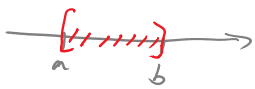
\includegraphics[width=3cm]{Bilder/83} \\
	halboffene Intervalle & $]a;b]$ & $\{a<x\le b\}$ & 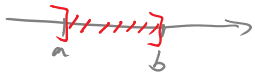
\includegraphics[width=3cm]{Bilder/84} \\
	& $[a;b[$ & $\{a\le x<b\}$ & 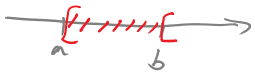
\includegraphics[width=3cm]{Bilder/85} \\
	offene Intervalle & $]a;b[$ & $\{a<x<b\}$ & 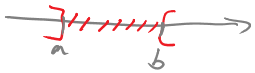
\includegraphics[width=3cm]{Bilder/86} \\
\end{longtable}

statt $]a;b]$ schreibt man auch $(a;b]$\\
statt $[a;b[$ schreibt man auch $[a;b)$\\
statt $]a;b[$ schreibt man auch $(a;b)$

\section{Uneigentliche Intervalle}
\begin{longtable}{lc}
	$]-\infty;a]$ & 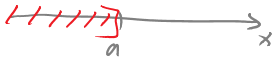
\includegraphics[width=3cm]{Bilder/87} \\
	$]-\infty;a[$ & 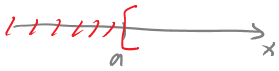
\includegraphics[width=3cm]{Bilder/88} \\
	$[a;\infty[$ & 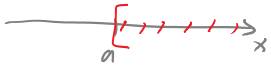
\includegraphics[width=3cm]{Bilder/89} \\
	$]a;\infty[$ & 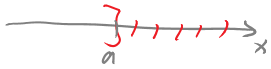
\includegraphics[width=3cm]{Bilder/90} \\
	$]-\infty;\infty[$ & 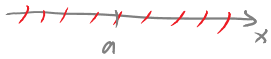
\includegraphics[width=3cm]{Bilder/91} \\
\end{longtable}

statt $]-\infty;a]$ schreibt man auch $(-\infty;a]$\\
statt $]-\infty;a[$ schreibt man auch $(-\infty;a)$\\
statt $[a;\infty[$ schreibt man auch $[a;\infty)$\\
statt $]a;\infty[$ schreibt man auch $(a;\infty)$\\
statt $]-\infty;\infty[$ schreibt man auch $(-\infty;\infty)$

\cleardoublepage
\part{Algebra und Arithmetik}
%\setcounter{chapter}{1}
\chapter{Zahlen}
\section{Ganze Zahlen und Teilbarkeit}
$\Z=\{0,\pm1, \pm2,\ldots\}$ Menge der ganzen Zahlen
\Def $t\in\Z$ heißt \ul{Teiler} von $a\in\Z$ (und $a$ \ul{Vielfaches} von $t$), wenn es ein $q\in\Z$ gibt mit \redbox{$a=q\cdot t$}\\
man schreibt dann $t|a$ ({\flqq $t$ teilt $a$\frqq} oder {\flqq $t$ ist Teiler von $a$\frqq})

\Bem $1$ und $a\in\Z$ sind stets Teiler von $a$; sie heißen \ul{triviale} (\ul{unechte}) Teiler von $a$; Teiler $t\ne 1$, $a$ heißen \ul{echte} Teiler von $a$.

\paragraph{Division mit Rest:} Für beliebige $a,b\in\Z,b\ne 0$, gibt es eindeutige ganze Zahlen $q,r\in\Z$ mit \\
\redbox{$a=q\cdot b+r$}\qquad und $0\le r<|b|$\\
$r$ heißt \ul{Rest} der Division von $a$ durch $b$ man schreibt $r=a\mod b$.

In $\Q$ gilt dann: \bluebox{$\dfrac{a}{b} = q + \dfrac{r}{b}$} (echter Bruch $r<|b|$, $q$: ganzzahliger Anteil)

\greenbox{$q=\Big\lfloor\dfrac{a}{b}\Big\rfloor$}

$\lfloor x\rfloor$ = untere Gauß-Klammer von $x$ = größte ganze Zahl $\le x$

\Bsps
$\lfloor 4{,}6\rfloor = 4 \qquad \lfloor -2{,}7\rfloor= -3$

\Bsps
\begin{enumerate}
	\item $a=14,b=5$\\
	$14=2\cdot 5+4\hfil \dfrac{14}{5} = 2+\dfrac{4}{5}$
	
	\item $a=-8, b=3$\\
	$-8=-3\cdot 3+1\hfil \dfrac{-8}{3} = -3+\dfrac{1}{3}$
	
	\Beachte Für den Rest $r$ muss stets $r\ge 0$ gelten ($0\le r<|b|$)
	
	\item $a = 16, b=-7$\\
	$16=-2\cdot (-7)+2\hfil \dfrac{16}{-7} = -2+\dfrac{2}{-7}$
	
	\item $a = -18, b=-15$\\
	$-18=-2\cdot (-15)+12\hfil \dfrac{-18}{-15} = -2+\dfrac{12}{-15}$
	
	\item $a = 328, b=14$\\
	%bild 1
	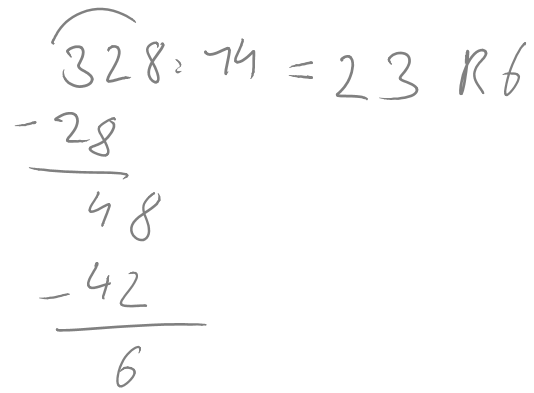
\includegraphics[width=5cm]{Bilder/71}\\
	$328=23\cdot 14 + 6\hfil \dfrac{328}{14} = 23+\dfrac{6}{14}$
	
	\item $a = -1024, b=23$\\
	%bild 2
	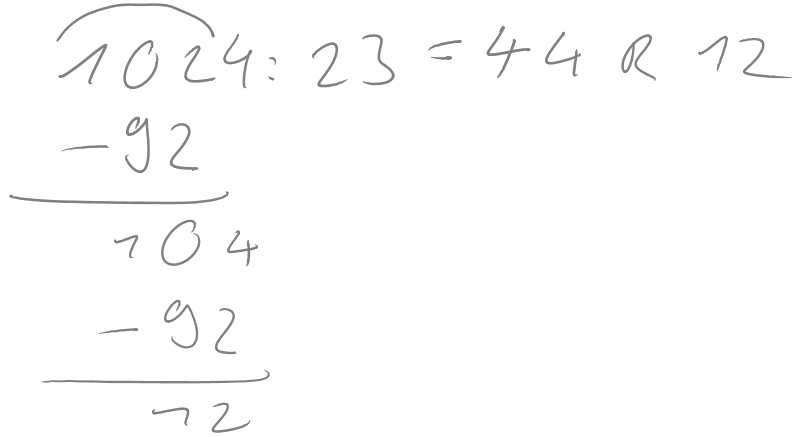
\includegraphics[width=5cm]{Bilder/70}\\
	$1024=44\cdot 23 + 12\\
	-1024=-44\cdot 23 - 12\\
	-1024=-45\cdot 23 + 11\hfil \dfrac{-1024}{23} = -45+\dfrac{11}{23}$
\end{enumerate}
	
\Def Eine \ul{Primzahl} ist eine natürliche Zahl $p\ge 2$, die keine echten Teiler besitzt.

\Bsp Primzahlen

$2,3,5,7,11,13,17,\ldots$

\Satz{{\bf Euklid}\\
	\\
	Es gibt unendlich viele Primzahlen}

\Theorem{{\bf Hauptsatz der elementaren Zahlentheorie}\\
	\\
	Jede ganze Zahl $a\in\Z,a\ne 0, \pm1$ kann eindeutig als Produkt von Primzahlen geschrieben werden, d.h.\\
	$a=\epsilon\cdot p_1^{e_1}\cdot\ldots\cdot p_k^{e_k}$\\
	mit $\epsilon\in\{\pm1\}$ und Primzahlen  $p_1<p_2<\ldots<p_k$ und Exponenten $e_1,\ldots,e_k\in\N$}

\Bsps
\begin{enumerate}
	\item $12 = 2^2\cdot 3$
	\item $-28 = -2^2\cdot 7$
	\item $-1024 = -2^{10}$
	\item $47293129 = 13^2\cdot 23^4$
\end{enumerate}

\Def
\begin{enumerate}
	\item $t$ heißt \ul{größter gemeinsamer Teiler} von $a$ und $b$ (i.Z. $t=\ggT(a,b)$, gcd), wenn $t$ ein Teiler von $a$ und $b$, und $t'|t$ für jeden gemeinsamen Teiler $t'$ von $a$ und $b$ gilt.
	
	\item $s$ heißt \ul{kleinstes gemeinsames Vielfaches} von $a$ und $b$, (i.Z. $s=\kgV(a,b)$, scm), wenn $s$ ein Vielfaches von $a$ und $b$ ist, und $s|s'$ für jedes gemeinsame Vielfache $s'$ von $a$ und $b$ gilt.
	
	\item $\ggT$ und $\kgV$ von mehr als zwei Zahlen sind analog definiert und es gilt:\\
	$\ggT(a_1, \ldots,a_n)=\ggT(\ggT(a_1, \ldots,a_{n-1}),a_n)$\\
	$\kgV(a_1, \ldots,a_n)=\kgV(\kgV(a_1, \ldots,a_{n-1}),a_n)$
\end{enumerate}

\Bem $\ggT$ und $\kgV$ sind bis auf das Vorzeichen eindeutig bestimmt, z.B. sind $5$ und $-5$ größte gemeinsame Teiler von $15$ und $20$;\\
oftmals bezeichnet man nur $t>0$ (bzw. $s>0$) als $\ggT$ (bzw. $\kgV$)

\Bem $\kgV(a_1,a_2)=\dfrac{a_1\cdot a_2}{\ggT(a_1,a_2)}$

\Satz{Seien $a,b\in\Z,a,b\ne0,\pm0$; wir schreiben\\
	$a=\epsilon p_1^{e_1}\cdot\ldots\cdot p_n^{e_n}$ und\\
	$b=\eta p_1^{f_1}\cdot\ldots\cdot p_n^{f_n}$\\
	mit $e,f\ge0$ und Primzahlen $p_1<\ldots<p_n$\\
	\\
	Dann gilt:\\
	$\ggT(a,b)=p_1^{\min(e_1,f_1)}\cdot\ldots\cdot p_n^{\min(e_n,f_n)}$\\
	$\kgV(a,b)=p_1^{\max(e_1,f_1)}\cdot\ldots\cdot p_n^{\max(e_n,f_n)}$}

\Bsps
\begin{enumerate}
	\item $a=12, b=18$\\
	$12 = 2^2\cdot 3$\\
	$18 = 2\cdot 3^2$\\
	$\ggT(12,18)=2\cdot3=6$\\
	$\kgV(12,18)=2^2\cdot3^2=36$
	
	\item $a=1400, b=1452$\\
	$1400 = 2^3\cdot 5^2\cdot 7 =  2^3\cdot 3^0\cdot 5^2\cdot 7\cdot 11^0$\\
	$1452 = 2^2\cdot 3\cdot 11^2 = 2^2\cdot 3\cdot 5^0\cdot 7^0\cdot 11^2$\\
	$\ggT(a,b)=2^2\cdot 3^0\cdot 5^0\cdot 7^0\cdot 11^0=4$\\
	$\kgV(a,b)=2^3\cdot 3\cdot 5^2\cdot 7\cdot 11^2=508200$
\end{enumerate}

\Def $a,b\in\Z,a,b\ne0$, heißen \ul{teilerfremd}, wenn $\ggT(a,b)=1$ gilt, d.h. wenn $a$ und $b$ keine gemeinsamen echten Teiler besitzen.

\Bsp $a=2^3\cdot5^2=200, b=3^2\cdot7=63$

\clearpage
\section{Euklidischer Algorithmus}
Der euklidischer Algorithmus ist ein effizientes Verfahren zur Bestimmung des größten gemeinsamen Teilers zweier ganzer Zahlen.

\paragraph{Euklidischer Algorithmus}
zur Berechnung von $\ggT(a,b),a,b\in\Z, b\ne0$.\\
Man führt fortlaufend Divisionen mit Rest durch, bis zum ersten Mal die Division aufgeht, d.h. der zugehörige Rest Null ist.

\begin{align*}
a &= q_1\cdot b + r_1\qquad& 0\le r_1<|b|\\
b &= q_2\cdot r_1 + r_2\qquad& 0\le r_2<r_1\\
r_1 &= q_3\cdot r_2 + r_3\qquad& 0\le r_3<r_2\\
&\vdots\\
r_{n-2} &= q_n\cdot r_{n-1} + r_n\qquad& 0\le r_n<r_{n-1}\\
r_{n-1} &= q_{n+1}\cdot r_n + 0\qquad& 0= r_{n+1}<r_n\\
\end{align*}

Division geht zum ersten Mal auf, d.h. $r_{n+1} = 0$

Dann gilt: \redbox{$r_n = \ggT(a,b)$}

\Bem
\begin{enumerate}
	\item Der Algorithmus terminiert (d.h. endet irgendwann) da $|b|>r_1>r_2>r_3>\ldots>r_n\ge 0$ gilt und somit die Folge der Reste $r_1,r_2,r_3,\ldots$ irgendwann Null wird.
	
	\item Wegen $\ggT(a,b)=\ggT(b,r_1)= \ggT(r_1,r_2)=\ldots = \ggT(r_{n-1},r_n) = \ggT(r_n, 0) = r_n$ ist der Algorithmus korrekt.
\end{enumerate}

\Bsps
\begin{enumerate}
	\item $\ggT(56,41)$
	\begin{align*}
	56 &=1\cdot \red{41}+\green{15}\\
	\red{41} &=2\cdot \green{15}+\blue{11}\\
	\green{15} &=1\cdot \blue{11}+\red{4}\\
	\blue{11} &=2\cdot \red{4}+\green{3}\\
	\red{4} &=1\cdot \green{3}+\blue{1} \leftarrow \ggT(56,41)\\
	\green{3} &=3\cdot \blue{1}+\green{0}
	\end{align*}
	$\Rightarrow \ggT(56,41) = 1$, d.h. 56 und 41 sind teilerfremd. 
	
	\item $\ggT(9625,9075)$
	\begin{align*}
	9625 &=1\cdot 9075+550\\
	9075 &=16\cdot 550+275 \leftarrow\ggT\\
	550 &=2\cdot 275+0\\
	\end{align*}
	$\Rightarrow \ggT(9625,9075) = 275$
	
\end{enumerate}

\Satz{{\bf Lineare Darstellung des $\ggT$}\\
	\\
	Zu $a,b\in\Z, b\ne0$, gibt es stets ganze Zahlen $p,q\in\Z$ mit\\
	\redbox{$pa+qb=\ggT(a,b)$}}

Der sogenannte \ul{erweiterte Euklidischer Algorithmus} bestimmt neben dem $\ggT(a,b)$ zusätzlich ganze Zahlen $p,a\in\Z$ mit $pa+qb=\ggT(a,b)$.

Man erhält die Koeffizienten $p$ und $q$ durch \ul{{\flqq Rückwärtseinsetzen\frqq}} im Divisionsschema des Euklidischen Algorithmus.

\Bsps
\begin{enumerate}
	\item $\ggT(56,41)$\\
	\begin{minipage}{0.3\linewidth}
		\begin{align*}
		\red{56} &=1\cdot \red{41}+15\\
		\green{41} &=2\cdot \green{15}+11\\
		\blue{15} &=1\cdot \blue{11}+4\\
		\red{11} &=2\cdot \red{4}+3\\
		\green{4} &=1\cdot \green{3}+1
		\end{align*}
	\end{minipage}
	\begin{minipage}{0.6\linewidth}
		\begin{align*}
		1 &=-4\cdot\green{41}+11\cdot(\red{56}-1\cdot \red{41}) = 11\cdot\red{56}-15\cdot\red{41}\\
		1 &=3\cdot\ \blue{15}-4\cdot(\green{41}- 2\cdot \green{15}) = -4\cdot\green{41}+11\cdot\green{15}\\
		1 &=-1\cdot\red{11}+3\cdot(\blue{15} - 1\cdot \blue{11}) = 3\cdot\ \blue{15}-4\cdot\blue{11}\\
		1 &= \green{4} - 1\cdot(\red{11} -2\cdot \red{4})= -1\cdot\red{11}+3\cdot\red{4}\\
		1 &= \green{4} - 1\cdot\green{3}
		\end{align*}
	\end{minipage}
	
	\item $\ggT(9625,9075)$\\
	%Equation 2 %bild 2
	\img{Bilder/67}{}{}	
\end{enumerate}

\clearpage
\section{Modulare Arithmetik, endliche Körper}
Wir hatten bereits die Äquivalenzrelation $\sim_n$ ($n\in\N$) auf $\Z$ wie folgt definiert: ($a,b\in\Z$)
\begin{align*}
a&\sim_n b\eq n|(a-b)
\end{align*}
(d.h. $n$ teilt $a-b$ bzw. $a-b$ ist durch $n$ teilbar)

statt $a\sim_nb$ schreibt man $a\equiv b \mod n$ und spricht {\flqq $a$ kongruent $b$ modulo $n$\frqq}.

Die Äquivalenzklassen $[a]$ ($a\in\Z$) (wir schreiben auch $\ol{a}$ statt $[a]$) nennt man \\\ul{Kongruenz- oder Restklassen modulo $n$};\\
ein vollständiges Repräsentantensystem ist $[0],[1][2],\ldots,[n-1]$;\\
dabei besteht die Klasse $[r]$ (=$\ol{r}$) aus allen ganzen Zahlen, die bei Division durch $n$ den Rest $r$ ergeben.

\begin{align*}
[0] &= \{k\cdot n\mid k\in\Z\}\\
[1] &= \{1+k\cdot n\mid k\in\Z\}\\
[2] &= \{2+k\cdot n\mid k\in\Z\}\\
&\vdots\\
[n-1] &= \{n-1+k\cdot n\mid k\in\Z\}\\
\end{align*}

Für die Restklassen definiert man Addition und Multiplikation wie folgt: (Definition erfolgt \ul{repräsentantenweise})

\begin{align*}
[a]+[b]&:=[a+b]\qquad (\text{bzw. }\ol{a}+\ol{b}= \ol{a+b})\\
[a]\cdot[b]&:=[a\cdot b]\qquad (\text{bzw. }\ol{a}\cdot\ol{b}= \ol{a\cdot b})\\
\end{align*}

Man kann zeigen, dass die Definitionen von der Wahl der Repräsentanten der Klassen nicht abhängen.\\
($\Rightarrow$ Addition und Multiplikation sind wohldefiniert)

\Satz{{\bf Definition:}\\
	die Menge $\Z/n\Z =\{[0],[1],\ldots,[n-1]\}$ zusammen mit obiger Addition und Multiplikation ist ein sogenannter Ring und heißt \ul{Restklassenring modulo $n$}.\\
	Die auf $\Z/n\Z$ definierte Arithmetik nennt man \ul{modulare Arithmetik} (anschaulich manchmal auch \ul{{\flqq Zeigerarithmetik\frqq}})}

\gray{$(\Z , + , \cdot) \entspricht$ Ring}

\Def Eine Menge $R$ zusammen mit zwei Verknüpfungen $+:R\times R\to R,(a,b)\mapsto a+b$, $\cdot:R\times R\to R,(a,b)\mapsto a\cdot b$ heißt (kommutativer) \ul{Ring} (mit Eins), wenn folgendes gilt:

\begin{enumerate}
	\item $a+b = b+a$\\
	$a\cdot b = b\cdot a$ \hfill Kommutativität
	
	\item $a+(b+c) = (a+b)+c$\\
	$a\cdot(b\cdot c) = (a\cdot b)\cdot c$ \hfill Assoziativität
	
	\item $a(b+c) = ab + ac$ \hfill Distributivität
	
	\item Existenz neutraler Elemente
	\begin{itemize}
		\item additives neutrales Element\\
		es existiert ein Element $0\in R$ mit $a+0=0+a=a$ für alle $a\in R$
		\item multiplikatives neutrales Element\\
		es existiert ein Element $1\in R$ mit $a\cdot 1=1\cdot a=a$ für alle $a\in R$
	\end{itemize}
	
	\item Existenz additiver inverser Elemente\\
	zu jedem $a\in R$ existiert ein additives inverses Element $-a$ mit $a+(-a) = (-a)+a = 0$
	
	Definiere die Subtraktion durch $a-b:=a+(-b)$
	
	\item Existenz multiplikativer inverser Elemente\\
	zu jedem $a\in R, a\ne 0$ existiert ein multiplikatives inverses Element $\inv{a}(=\frac{1}{a})$ mit $a\cdot \inv{a} = \inv{a}\cdot a = 1$ heißt $R$ \ul{Körper}.
\end{enumerate}

\Bsp \quad\\
($\N,+,\cdot$) ist \ul{kein} Ring (es fehlen die additiven inversen Elemente)\\
($\Z,+,\cdot$) ist ein Ring, aber \ul{kein} Körper (es fehlen die multiplikativen inversen Elemente)\\
($\Q,+,\cdot$) ist ein Körper\\
($\R,+,\cdot$) ist ein Körper\\
($\C,+,\cdot$) ist ein Körper\\


\Bsps
\begin{enumerate}
	\item $\Z/2\Z=\{\ol{0}, \ol{1}\}$
	\begin{align*}
	\ol{0}+\ol{1} &= \ol{0+1} = \ol{1}\\
	\ol{1}+\ol{1} &= \ol{1+1} = \ol{2} = \ol{0}\\
	\end{align*}
	
	\item $\Z/12\Z=\{\ol{0}, \ol{1}, \ol{2}, \ol{3}, \ldots, \ol{11}\}$
	\begin{align*}
	\ol{2}+\ol{3} &= \ol{2+3} = \ol{5}\\
	\ol{2}+\ol{11} &= \ol{2+11} = \ol{13} = \ol{1}\\
	\ol{4}+\ol{10} &= \ol{4+10} = \ol{14} = \ol{2}\\
	\end{align*}
	%bild 3
	\imgw{Bilder/60}{{\flqq Zeigerarithmetik\frqq}Uhr}{}{5cm}
\end{enumerate}

in $\Z/12\Z$ gibt es sogenannte \ul{Nullteiler} (in $\Z$ gibt es diese nicht)\\
$\ol{3} \cdot \ol{4} = \ol{3\cdot 4}= \ol{12} = \ol{0}$ ($\ol{3}$ und $\ol{4}$ sind \ul{Nullteiler})\\
$\ol{3}\ne \ol{0}$ und $\ol{4}\ne \ol{0}$, jedoch ist das Produkt $\ol{3} \cdot \ol{4}$ gleich $\ol{0}$ (\red{Vorsicht!})\\
d.h. aus $\ol{a} \cdot \ol{b} = \ol{0}$ folgt i.a. \ul{nicht} $\ol{a} = 0$ oder $\ol{b} = 0$

\Satz{Für jede Primzahl $p$ ist $\Z/p\Z$ ein Körper er heißt \ul{endlicher Körper} (oder Galoriskörper) mit $p$ Elementen und wird mit $\F_p$ (oder $\GF(p)$) bezeichnet.}

\Bem allgemein gibt es genau zu jeder Primzahlpotenz $p^n$ genau einen endlichen Körper $\GF(p^n)$ mit $p^n$ Elementen ($\GF(p^n) \ne \Z/p^n\Z$ für $n>1$)

\Bem In $\Z/p\Z = \{\ol{0},\ol{1},\ldots,\ol{p-1}\}$ gibt es zu $\ol{1},\ol{2},\ldots,\ol{p-1}$ jeweils ein multiplikatives Inverses; diese erhält man mithilfe des erweiterten Euklidischen Algorithmus.

\Satz{Mithilfe des erweiterten Euklidischen Algortihmus findet man zu $\ol{a}\in\Z/p\Z, \ol{a}\ne\ol{0}$ ganze Zahlen $s,t\in\Z$ mit\\
	$sa+tp=1$.\\
	Dann ist $\ol{s}$ das multiplikative Inverse zu $\ol{a}$, d.h. $\ol{s}=\inv{\ol{a}}$}

\Beweis Da $\ol{a}\ne\ol{0}$ gilt, ist $a$ durch $p$ \ul{nicht} teilbar\\
d.h. die Primzahl $p$ kommt in der Primfaktorisierung von $a$ nicht vor $\Rightarrow\ggT(a,p)=1$\\
aus linearer Darstellung des $\ggT$ folgt\qquad $sa+tp=1$\\
für gewisse $s,t\in\Z$.

Bildet man die Restklassen, so folgt
\begin{align*}
\ol{sa+tp}&=\ol{1}\\
\ol{s}\cdot\ol{a}+\underbrace{\ol{t}\cdot\underbrace{\ol{p}}_{\ol{0}}}_{\ol{0}}&=\ol{1}\\
\ol{s}\cdot\ol{a}&=\ol{1}\\
\end{align*}
d.h. $\ol{s}=\inv{\ol{a}}$

\Bsps
\begin{enumerate}
	\item $\Z/3\Z=\{\ol{0},\ol{1},\ol{2}\}$\\
	\begin{align*}
	\ol{1}\cdot\ol{1} &=\ol{1\cdot 1} = \ol{1} \Rightarrow \inv{\ol{1}} = \ol{1}\\
	\ol{2}\cdot\ol{2} &=\ol{2\cdot 2} = \ol{4} = \ol{1} \Rightarrow \inv{\ol{2}} = \ol{2}\\
	\end{align*}
	
	\item $\Z/5\Z=\{\ol{0},\ol{1},\ol{2},\ol{3},\ol{4}\}$\\
	\begin{align*}
	\inv{\ol{1}} &= \ol{1}\\
	\ol{2}\cdot\ol{3} &=\ol{2\cdot 3} = \ol{6} = \ol{1} \Rightarrow \inv{\ol{2}} = \ol{3}\\
	\ol{4}\cdot\ol{4} &=\ol{4\cdot 4} = \ol{16} = \ol{1} \Rightarrow \inv{\ol{4}} = \ol{4}\\
	\end{align*}
	
	\item $\Z/17\Z=\{\ol{0},\ol{1},\ol{2},\ldots,\ol{16}\}$\\
	Bestimme das multiplikative Inverse von $\ol{15}$ (in $\Z/17\Z$)\\
	$\ggT(17,15) = 1 \stackrel{\text{erw. Eukl. Alg.}}{\Longrightarrow} s\cdot15+t\cdot17 = 1; \ol{s} = \inv{\ol{15}}$
	\begin{align*}
	17 &= 1\cdot 15 + 2 &\Rightarrow 1= 15-7\cdot (17-1\cdot 15) = -7\cdot 17+8\cdot 15\\
	15 &= 7\cdot 2 + 1_{\ggT} &\Rightarrow 1= 15-7\cdot 2\\
	\end{align*}
	
	$\Rightarrow 8\cdot 15 -7\cdot 17 = 1$ (lineare Darstellung des $\ggT$)
	$\ol{8} = \inv{\ol{15}}$ \ul{Probe}: $\ol{8\cdot 15} = \ol{120} = \ol{7\cdot17\cdot +1} = \ol{1}$
	
	\item $\Z/1013\Z=\{\ol{0},\ol{1},\ol{2},\ldots,\ol{1012}\}$\\
	Bestimme das multiplikative Inverse von $\ol{1000}$ (in $\Z/1013\Z$)\\
	%bild 4
	\img{Bilder/66}{}{}
\end{enumerate}

\clearpage
\section{Stellenwertsysteme}
\ul{Stellenwertsystem} = Zahlensystem, bei dem Zahlen durch eine Folge von Symbolen (Ziffern) dargestellt werden und die Wertigkeit eines Symbols auch von seiner Position (=Stelle) in der Folge abhängt.

\paragraph{b-adische Zahlensysteme} sind spezielle Stellenwertsysteme ($b\in\N, b\ge2$)
\begin{itemize}
	\item $b$ Ziffern: $0,1,2,\ldots,9,A,B,C,D,\ldots$ ($b$-adische Ziffern)
	
	\item Wertigkeit der $i$-ten Ziffer an der $j$-ten stelle (von rechts nach links gezählt) ist gleich
	\redbox{$(i-1)\cdot b^{j-1}$}
	Wert der reinen Ziffer
	Gewicht der j-ten Stelle
	%bild 5
	\imgw{Bilder/61}{}{}{11cm}
\end{itemize}

\Satz{Sei $b\in\N,b\ge2$. Dann besitzt jede ganze Zahl $n\ge1$ eine eindeutige Darstellung in der Form\\
	$(a_ra_{r-1}\ldots a_0)_b$\\
	mit $b$-adischen Ziffern $a_0,\ldots,a_r (a_r\ne0)$; sie heißt $b$-adische Darstellung von $n$. Ihr Wert berechnest sich durch\\
	\greenbox{$n=\sum\limits_{i=0}^{r}a_i\cdot b^i$} \qquad $a_i$: Wert der reinen Ziffer}

\clearpage
\Bsp
\begin{enumerate}
	\item Dualsystem (2-adisch)\\
	Ziffern: $0,1$
	%bild 6
	\imgw{Bilder/62}{}{}{8cm}
	
	\item Oktalsystem (8-adisch)\\
	Ziffern: $0,1,2,3,4,5,6,7$
	%bild 7
	\imgw{Bilder/63}{}{}{7cm}
	\begin{minipage}{\linewidth}
		\Bluebox{
		\centering
		{\flqq OCT 31 = DEC 25\frqq}(Joke)\\
		Halloween = Weihnachten}
	\end{minipage}
	
	\item Dezimalsystem (10-adisch)\\
	Ziffern: $0,1,2,3,4,5,6,7,8,9$
	%bild 8
	\imgw{Bilder/64}{}{}{10cm}
	
	\item Hexadezimalsystem (16-adisch)\\
	Ziffern: $0,1,2,3,4,5,6,7,8,9,A,B,C,D,E,F$
	%bild 9
	\imgw{Bilder/65}{}{}{9cm}
\end{enumerate}

\clearpage
\subsection{Umrechnen Dezimaldarstellung in b-adische Darstellung}
Fortlaufende Division durch $b$ (mit Rest) liefert von rechts nach links die Ziffern der $b$-adischen Darstellung (aus den Resten der Division).

\begin{align*}
n &= q_1\cdot b + r_1\qquad& 0\le r_1<b\\
q_1 &= q_2\cdot b + r_2\qquad& 0\le r_2<b\qquad q_1 \ne 0\\
q_2 &= q_3\cdot b + r_3\qquad& 0\le r_3<b\qquad q_2 \ne 0\\
&\vdots\\
q_{s-2} &= q_{s-1}\cdot b + r_{s-1}\qquad& 0\le r_{s-1}<b\qquad q_{s-1} \ne 0\\
q_{s-1} &= q_s\cdot b + r_s\qquad& 0< r_s<b\qquad q_s = 0\\
\end{align*}

$n\entspricht (r_s\ldots r_1)_b$

Algorithmus terminiert da\\
$q_1>q_2>\ldots>q_{s-1}>q_s=0$

\clearpage
\Bsps
\begin{enumerate}
	\item $287\rightarrow$ 2-adisch\\
	\begin{align*}
	287&= 143\cdot 2 + 1\\
	143&= 71\cdot 2 + 1\\
	71&= 35\cdot 2 + 1\\
	35&= 17\cdot 2 + 1\\
	17&= 8\cdot 2 + 1\\
	8&= 4\cdot 2 + 0\\
	4&= 2\cdot 2 + 0\\
	2&= 1\cdot 2 + 0\\
	1&= 0\cdot 2 + 1\\
	\Rightarrow 287 &= (100011111)_2\\
	\end{align*}
	Probe: $1+2+4+8+16+256 = 287$
	
	\item $287\rightarrow$ 8-adisch\\
	\begin{align*}
	287&= 35\cdot 8 + 7\\
	35&= 4\cdot 8 + 3\\
	4&= 0\cdot 8 + 4\\
	\Rightarrow 287 &= (437)_8
	\end{align*}
	
	\item $287\rightarrow$ 16-adisch\\
	\begin{align*}
	287&= 17\cdot 16 + 15\\
	17&= 1\cdot 16 + 1\\
	1&= 0\cdot 16 + 1\\
	\Rightarrow 287 &= (11F)_{16}\\
	\end{align*}
\end{enumerate}

\Bem In der Regel muss man/sollte man bei Umrechnungen von einem Zahlensystem in ein anderes den Weg über das Dezimalsystem wählen.

\paragraph{Ausnahme:} 2-adisch $\leftrightarrow$ 16-adisch

\Idee $\underbrace{\square\square\square\square}_\text{im Dualsystem} \entspricht \underbrace{\square}_\text{im Hexadezimalsystem}$

Zerlege (von rechts beginnend) die Dualzahl in Gruppen von jeweils 4 benachbarten Bits und rechne jeder 4er Gruppe in eine Hexadezimalziffer um.

$\underbrace{\square\square\square\square}_\square\underbrace{\square\square\square\square}_\square\underbrace{\square\square\square\square}_\square\underbrace{\square\square\square\square}_\square {\color{white}\underbrace{\color{black}\text{2-adisch}}_{\color{black}\text{16-adisch}}}$

Erzeuge aus jeder Ziffer aus dem Hexadezimalsystem ein 4-Bit-Muster und füge diese zu einer Dualzahl zusammen. Streiche führende Nullen.

\chapter{Gleichungen und Ungleichungen}
\section{Definitionen}
\begin{itemize}
	\item \ul{Term} (induktive Definition)
	\begin{enumerate}
		\item Variablen und Zahlen (=Konstanten) sind Terme (atomare Terme)
		\item Sind $T_1$ und $T_2$ Terme, so sind $T_1+T_2, T_1-T_2, T_1\cdot T_2, T_1:T_2, \dfrac{T_1}{T_2}, (T_1)$ Terme
		\item Sind $T_1,\ldots,T_r$ Terme und ist $f$ ein $r$-stelliges Funktionszeichen, so ist auch $f(T_1,\ldots,T_r)$ ein Term
		\item Keine weiteren Zeichenketten sind Terme
	\end{enumerate}
	\Bsp $5,x_1, x_1+x_2, \sin(5x_1+x_2-x_3),\sqrt{x_1^2+x_2^2}$
	\paragraph{Bezeichnung:} Sind die Variablen eines Terms $T$ in der Menge $\{x_1,\ldots,x_n\}$ enthalten, so schreiben wir $T(x_1,\ldots,x_n)$
	
	\clearpage
	\item \ul{Äquivalenz} zweier Terme
	
	Zwei Terme $T_1(x_1,\ldots,x_n)$ und $T_2(x_1,\ldots,x_n)$ heißen \ul{äquivalent über einer Grundmenge} $\G\subseteq \R^n$ (bzw. $\G\subseteq\C^n$) $T_1(a_1,\ldots,a_n) = T_2(a_1,\ldots,a_n)$ für \ul{alle} $(a_1,\ldots,a_n) \in \G$ gilt; i.Z. $T_1(x_1,\ldots,x_n) \underset{\G}{\equiv} T_2(x_1,\ldots,x_n)$ bzw. (unpräziser formuliert) $T_1(x_1,\ldots,x_n) = T_2(x_1,\ldots,x_n)$ (über $\G$)
	
	\Bsps
	\begin{enumerate}
		\item $x^2+2x+1 = (x+1)^2$\qquad über $\G = \R$
		\item $\dfrac{x^2+x}{2x} = \dfrac{x+1}{2}$\qquad über $\G = \R\setminus\{0\} = \{x\ne0\}$
		\item $\dfrac{x_1^2+x_2}{x_1} = x_1\cdot x_2$\qquad über $\G = (\R\setminus\{0\})\times\R \subseteq\R^2= \{(x_1,x_2)\mid x_1\ne0\} = \{x\ne0\}$
		\item $\sqrt{x^2} = |x|$\qquad über $\G = \Rop = \{x\ge0\}$
		\item $e^{2\ln(x)} = x^2$\qquad über $\G = \Rp = \{x>0\}$
	\end{enumerate}
	
	\clearpage
	\item \ul{Gleichung/Ungleichung}
	
	Eine \ul{Gleichung} (bzw. \ul{Ungleichung}) in den unbestimmten $x_1,\ldots,x_n$ übe einer Grundmenge $\G\subseteq\R^n$ (oder $\G\subseteq\C^n$) ist ein formaler Ausdruck der Form $T_1(x_1,\ldots,x_n) \square T_2(x_1,\ldots,x_n)$ wobei $T_1(x_1,\ldots,x_n)$ und $T_2(x_1,\ldots,x_n)$ Terme sind und $\square$ für $=$ (bzw. $\le,\ge,<,>$) steht.
	
	Eine \ul{Lösung} obiger Gleichung (bzw. Ungleichung) ist ein $n$-Tupel $(a_1,\ldots,a_n)\in\G$, so dass $T_1(a_1,\ldots,a_n) \square T_2(a_1,\ldots,a_n)$ eine wahre Aussage ist; mit $\L=\{(a_1,\ldots,a_n)\in\G\mid(a_1,\ldots,a_n)\text{ ist Lösung}\}\subseteq\G$ bezeichnen wir die \ul{Lösungsmenge} der Gleichung (bzw. Ungleichung).
	
	\Bem $\L$ hängt wesentlich von der Wahl der Unbestimmten $x_1,x_2,\ldots,x_n$ und der Grundmenge $\G$ ab.

	\clearpage
	\Bsps
	\begin{enumerate}
		\item Gleichung $2x_1 = 5$ in $x_1$ über $\G=\Z$\\
		$\Rightarrow \L=\emptyset$
		\item Gleichung $2x_1 = 5$ in $x_1$ über $\G=\Q$\\
		$\Rightarrow \L=\{\frac{5}{2}\}$
		\item Gleichung $2x_1 = 5$ in $x_1,x_2$ über $\G=\R^2$\\
		$\Rightarrow \L=\{(x_1,x_2)\mid x_1=\frac{5}{2}, x_2\in\R\}\subseteq\R^2$
		\imgw{Bilder/68}{}{}{10cm}
	\end{enumerate}
	
	\Def Zwei Gleichungen $\varphi_1$ und $\varphi_2$ in den Unbestimmten $x_1,\ldots,x_n$ über einer (gemeinsamen) Grundmenge $\G$ heißen \ul{äquivalent}, wenn sie übereinstimmende Lösungsmenge besitzen; i.Z. $\varphi_1\Leftrightarrow\varphi_2$
	
	\clearpage
	\item \ul{Äquivalenzumformungen}
	
	\begin{longtable}{c|c|c}
		\parbox{0.3\linewidth}{\vspace{2em}Äquivalenzumformung\vspace{2em}} &
		\parbox{0.25\linewidth}{\vspace{2em}Gleichung\\$T_1=T_2$\vspace{2em}} &
		\parbox{0.5\linewidth}{\vspace{2em}Ungleichung $T_1\le T_2$\\(analog für $T_1\ge T_2,T_1 < T_2,T_1 > T_2$)\vspace{2em}}\\
		\hline
		
		\parbox{0.25\linewidth}{\vspace{2em}Vertauschen beider Seiten\vspace{2em}} &
		\parbox{0.25\linewidth}{\vspace{2em}${\color{white}\Leftrightarrow}T_1 = T_2\\\Leftrightarrow T_2 = T_1$\vspace{2em}} &
		\parbox{0.5\linewidth}{\vspace{2em}${\color{white}\Leftrightarrow}T_1 \le T_2\\\Leftrightarrow T_2 \ge T_1$\vspace{2em}}\\
		
		\parbox{0.25\linewidth}{\vspace{2em}Seite(n) durch\\
			(über $\G$) äquivalente Terme ersetzen\\
			($T_1'=T_1$ über $\G$\\
			$T_2'=T_2$ über $\G$)\vspace{2em}} &
		\parbox{0.25\linewidth}{\vspace{2em}${\color{white}\Leftrightarrow}T_1 = T_2\\\Leftrightarrow T_1' = T_2'$\vspace{2em}} &
		\parbox{0.5\linewidth}{\vspace{2em}${\color{white}\Leftrightarrow}T_1 \le T_2\\\Leftrightarrow T_1' \le T_2'$\vspace{2em}}\\
		
		\parbox{0.25\linewidth}{\vspace{2em}Addition bzw. Subtraktion mit einem Term $T$\vspace{2em}} &
		\parbox{0.25\linewidth}{\vspace{2em}${\color{white}\Leftrightarrow}T_1 = T_2\mid\pm T\\\Leftrightarrow T_1\pm T = T_2\pm T$\vspace{2em}} &
		\parbox{0.5\linewidth}{\vspace{2em}${\color{white}\Leftrightarrow}T_1 \le T_2\mid\pm T\\\Leftrightarrow T_1\pm T \le T_2\pm T$\vspace{2em}}\\
		
		\parbox{0.25\linewidth}{\vspace{2em}Multiplikation mit bzw. Division durch eine Zahl $a\ne0$\vspace{2em}} &
		\parbox{0.25\linewidth}{\vspace{2em}${\color{white}\Leftrightarrow}T_1 = T_2\mid\cdot: a\\\Leftrightarrow T_1\cdot a = T_2\cdot a\\\Leftrightarrow \dfrac{T_1}{a} = \dfrac{T_2}{a}$\vspace{2em}} &
		\parbox{0.25\linewidth}{\vspace{2em}\grayframe{$a>0$}\\${\color{white}\Leftrightarrow}T_1 \le T_2\mid\cdot: a\\\Leftrightarrow T_1\cdot a \le T_2\cdot a\\\Leftrightarrow \dfrac{T_1}{a} \le \dfrac{T_2}{a}$\vspace{2em}}
		\parbox{0.25\linewidth}{\vspace{2em}\grayframe{$a<0$}\\${\color{white}\Leftrightarrow}T_1 \le T_2\mid\cdot: a\\\Leftrightarrow T_1\cdot a \ge T_2\cdot a\\\Leftrightarrow \dfrac{T_1}{a} \ge \dfrac{T_2}{a}$\vspace{2em}}\\
	\end{longtable}
	
	\clearpage
	\item \ul{Umformungen}, die i.a. \ul{keine} Äquivalenzumformungen sind
	\begin{enumerate}
		\item Multiplikation mit bzw. Division durch einen Term\\
		Da eine Division durch $T$ einer Multiplikation mit $\dfrac{1}{T}$ entspricht, betrachten wir im folgenden nur die \ul{Multiplikation mit einem Term $T$}.
		
		Uneingeschränkter Gebrauch der Multiplikation mit einem Term kann zu Widersprüchen führen, wie z.B. $x-1 = 0\mid \cdot \dfrac{x-2}{x-1}(=T)\Leftrightarrow x-2=0$ \red{$\Rightarrow$ Vorsicht!!!}
		
		\ul{Gleichung}\qquad $T_1=T_2$ \qquad über $\G$\\
		will man die Gleichung mit einem Term $T$ multiplizieren, so ist dies nur dann eine Äquivalenzumformung, wenn $T$ auf $\G$ definiert (d.h. $\G\subseteq\D_T$ = Definitionsmenge von $T$) und $T\ne0$ auf $\G$ gilt.\\
		Ansonsten sind Fallunterscheidungen nötig, bei der die Grundmenge $\G$ unterschiedlich eingeschränkt wird.
		
		$T_1=T_2$ (über $\G$) (mit $T$ multipliziert)
		%bild 10
		\imgw{Bilder/69}{}{}{8cm}
		\clearpage
		Für die Lösungsmenge $\L$ gilt:\\
		$\L = \L_1 \cup \L_2 \cup \L_3$
		
		\Bsps
		\begin{enumerate}
			\item $x^2 = 3x$ über $\G=\R$\\
			mit $T=\dfrac{1}{x}$ multiplizieren; $\D_T = \{x\ne0\}$
			
			%bild 101
			\ul{1.Fall:} $\G_1$\parbox[t]{5cm}{$=\G\cap \D_T\cap\{T\ne0\}\\=\R\cap \{x\ne0\}\cap\R \\= \{x\ne0\}$}
			\begin{align*}
			x^2 &= 3x \mid \cdot \dfrac{1}{x}\quad(\ne0)\\
			\Leftrightarrow x &= 3\in\G_1\\
			\Rightarrow\L_1 &=\{3\}
			\end{align*}
			
			\ul{2.Fall:} $\G_2$\parbox[t]{5cm}{$=\G\cap \D_T\cap\{T=0\}\\=\R\cap \{x\ne0\}\cap\emptyset \\= \emptyset$}
			\begin{align*}
			\Rightarrow\L_2 &=\emptyset
			\end{align*}
			
			\ul{3.Fall:} $\G_3$\parbox[t]{5cm}{$=\G\setminus \D_T\\=\R\setminus \{x\ne0\} \\= \{x=0\}$}
			\begin{align*}
			x^2 &= 3x\\
			x &= 0 \text{ in obige Gleichung eingesetzt}\Rightarrow 0=0\\
			\Rightarrow \text{jedes Element aus }&\G_3\text{ ist Lösung}\\
			\Rightarrow\L_3 &=\{0\}
			\end{align*}
			
			\ul{insgesamt:}
			\begin{align*}
			\Rightarrow\L &=\L_1\cup\L_2\cup\L_3\\
			&= \{0;3\}
			\end{align*}
						
			\Bem Versuche Multiplikation mit bzw. Division durch einen Term zu vermeiden, z.B.
			\begin{align*}
			x^2 &= 3x\\
			\Leftrightarrow x^2-3x &= 0\\
			\Leftrightarrow x(x-3) &= 0\\
			\Leftrightarrow x=0 &\lor x-3=0\\
			\L &=\{0;3\}
			\end{align*}
			
			\item $x-1 = 0$ über $\G=\R$\\
			Wir wollen unbedingt die Gleichung mit $\dfrac{x-2}{x-1}$ multiplizieren\\
			($x-1=0\mid\dfrac{x-2}{x-1} \Leftrightarrow x-2 = 0$, uneingeschränkter Gebrauch $\rightarrow$ Widersprüche)
			
			%bild 102
			$T=\dfrac{x-2}{x-1}\qquad\D_T=\R\setminus\{1\}=\{x\ne1\}$
			
			\ul{1.Fall:} $\G_1$\parbox[t]{5cm}{$=\G\cap \D_T\cap\{T\ne0\}\\=\R\cap \{x\ne1\}\cap\{x\ne2\} \\= \{x\ne1,x\ne2\}$}
			\begin{align*}
			x-1 &= 0 \mid \cdot \dfrac{x-2}{x-1}\quad(\ne0)\\
			\Leftrightarrow x-2 &= 0\\
			\Leftrightarrow x &= 2\not\in\G_1\\
			\Rightarrow\L_1 &= \emptyset
			\end{align*}
			
			\ul{2.Fall:} $\G_2$\parbox[t]{5cm}{$=\G\cap \D_T\cap\{T=0\}\\=\R\cap \{x\ne1\}\cap\{x=2\} \\= \{x=2\}$}
			\begin{align*}
			x-1 &= 0\\
			x &= 2\qquad\red{!!!}\\
			\Rightarrow\L_2 &=\emptyset
			\end{align*}
			
			\ul{3.Fall:} $\G_3$\parbox[t]{5cm}{$=\G\setminus \D_T\\=\R\setminus \{x\ne1\} \\= \{x=1\}$}
			\begin{align*}
			x-1 &= 0\\
			x &= 1\text{ in obige Gleichung eingesetzt}\Rightarrow 0=0\\
			\Rightarrow \text{jedes Element aus }&\G_3\text{ ist Lösung}\\
			\Rightarrow\L_3 &=\{1\}
			\end{align*}
			
			\ul{insgesamt:}
			\begin{align*}
			\Rightarrow\L &=\L_1\cup\L_2\cup\L_3\\
			&= \{1\}
			\end{align*}
		\end{enumerate}
		
		\clearpage
		\ul{Ungleichung}\qquad $T_1\le T_2$ \qquad über $\G$\\
		will man die Ungleichung mit einem Term $T$ multiplizieren, so ist dies nur dann eine Äquivalenzumformung, wenn $T$ auf $\G$ definiert (d.h. $\G\subseteq\D_T$ = Definitionsmenge von $T$) und $T\ne0$ auf $\G$ gilt.\\
		Ansonsten sind Fallunterscheidungen nötig, bei der die Grundmenge $\G$ unterschiedlich eingeschränkt wird.
		
		$T_1\le T_2$ (über $\G$) (mit $T$ multipliziert)
		%bild \ldots
		\imgw{Bilder/76}{}{}{11cm}
		\clearpage
		Für die Lösungsmenge $\L$ gilt:\\
		$\L = \L_1 \cup \L_2 \cup \L_3 \cup \L_4$
		
		\Bsps
		\begin{enumerate}
			\item $\dfrac{x^2 -3x +2}{x-1} \ge 0$ über $\G=\R\setminus\{1\}=\{x\ne1\}$\\
			mit $T=x-1$ multiplizieren; $\D_T = \R$
			
			\ul{1.Fall:} $\G_1$\parbox[t]{5cm}{$=\G\cap \D_T\cap\{T>0\}\\=\{x\ne1\}\cap\R\cap \{x>1\} \\= \{x>1\}$}
			\begin{align*}
			\dfrac{x^2 -3x +2}{x-1} &\ge 0 \mid \cdot (x-1)\quad(>0)\\
			\Leftrightarrow x^2 -3x +2 &\ge 0\\
			\text{Nullstelle von }x^2 -3x +2\\
			x_{1/2} &= \dfrac{3\pm\sqrt{9-4\cdot2}}{2}\\
			&= \dfrac{3\pm1}{2}\\
			x_1 = 1, x_2 = 2
			\end{align*}
			\imgw{Bilder/77}{}{}{5cm}
			\begin{align*}
			\Rightarrow\L_1 &=\{x\ge2\}
			\end{align*}
			
			\ul{2.Fall:} $\G_1$\parbox[t]{5cm}{$=\G\cap \D_T\cap\{T<0\}\\=\{x\ne1\}\cap\R\cap \{x<1\} \\= \{x<1\}$}
			\begin{align*}
			\dfrac{x^2 -3x +2}{x-1} &\ge 0 \mid \cdot (x-1)\quad(<0)\\
			\Leftrightarrow x^2 -3x +2 &\le 0\\
			\end{align*}
			\imgw{Bilder/78}{}{}{5cm}
			\begin{align*}
			\Rightarrow\L_2 &=\emptyset
			\end{align*}
			
			\ul{3.Fall:} $\G_3$\parbox[t]{5cm}{$=\G\cap \D_T\cap\{T=0\}\\=\{x\ne1\}\cap\R\cap \{x=1\} \\= \emptyset$}
			\begin{align*}
			\Rightarrow\L_3 &=\emptyset
			\end{align*}
			
			\ul{4.Fall:} $\G_4$\parbox[t]{5cm}{$=\G\setminus \D_T \\=\{x\ne1\}\setminus\R \\= \emptyset$}
			\begin{align*}
			\Rightarrow\L_4 &=\emptyset
			\end{align*}
			
			\ul{insgesamt:}
			\begin{align*}
			\Rightarrow\L &=\L_1\cup\L_2\cup\L_3\cup\L_4\\
			&= \{x\ge2\}
			\end{align*}
			
			\Bem
			\begin{align*}
			x2-3x+2 &= (x-1)(x-2)\\
			\dfrac{x^2 -3x +2}{x-1} &\ge 0 \qquad(x\ne1)\\
			\Leftrightarrow \dfrac{(x-1)(x-2)}{1\cdot(x-1)} &\ge 0\\
			\Leftrightarrow x-2 &\ge 0\\
			\Leftrightarrow x &\ge 2
			\end{align*}
		\end{enumerate}
		
		\item \ul{Anwenden einer Funktion $f(x)$ auf beiden Seiten} der Gleichung/Ungleichung
		
		\grayframe{Gleichung} $T_1=T_2$ über $\G$
		
		Will man auf beiden Seiten der Gleichung eine Funktion anwenden $f(x)$, so ist dies nur dann eine Äquivalenzumformung, wenn $f(x)$ auf $T_1(\G)\cup T_2(\G)$ (d.h. auf der linken und rechten Seite) definiert und injektiv (z.B. streng monoton steigend/fallend) ist.
		
		$T(\G)=\{T(a_1,\ldots,a_n)\mid(a_1,\ldots,a_n)\in\G\}$ Bildmenge von $T$
		
		Ist $f(x)$ auf $T_1(\G)\cup T_2(\G)$ definiert, aber nicht injektiv, so muss am Ende der Rechnung eine \ul{Probe} durchgeführt werden.
		
		\begin{align*}
		T_1 &= T_2\mid f(\ldots)\\
		\Rightarrow f(T_1)=f(T_2)\ldots \Rightarrow \L + \text{Probe!}
		\end{align*}
		Pfeil nur in eine Richtung da keine Äquivalenzumformung
		
		\Bsp 
		$\sqrt{x}, \ln x, e^x$ sind streng monoton steigend\\
		\Beachte $\sqrt{x}$ ist nur für $x\ge0$ und $\ln x$ ist nur für $x>0$ definiert. $x^2$ ist für $x\ge0$ streng monoton steigend und für $x\le0$ streng monoton fallend.
		
		\grayframe{Ungleichung} $T_1 \le T_2$ über $\G$
		(bzw. $T_1 < T_2$ über $\G$)
		
		Ist $f(x)$ auf $T_1(\G)\cup T_2(\G)$ definiert und
		\begin{itemize}
			\item streng monoton steigend, so rechne wie folgt\\
			\begin{align*}
			T_1 &\le T_2\mid f(\ldots)\\
			\Leftrightarrow f(T_1) &\le f(T_2)
			\end{align*}
			bzw.
			\begin{align*}
			T_1 &< T_2\mid f(\ldots)\\
			\Leftrightarrow f(T_1) &< f(T_2)
			\end{align*}
			
			\item streng monoton fallend, so rechne wie folgt\\
			\begin{align*}
			T_1 &\le T_2\mid f(\ldots)\\
			\Leftrightarrow f(T_1) &\ge f(T_2)
			\end{align*}
			bzw.
			\begin{align*}
			T_1 &< T_2\mid f(\ldots)\\
			\Leftrightarrow f(T_1) &> f(T_2)
			\end{align*}
			
			%bild 103
			\Bsp $\underbrace{x^2}_{\ge0} > \underbrace{4}_{\ge0}\\\sqrt{x}$ ist auf $x\ge0$ definiert und streng monoton steigend
			\begin{align*}
			x^2 & > 4\mid\sqrt{\quad}\\
			\Leftrightarrow \underbrace{\sqrt{x^2}}_{|x|} & > \sqrt{4}\\
			\Leftrightarrow |x| & > 2\\
			\Leftrightarrow x &> 2 \lor x < -2
			\end{align*}
			
			\graybox{\parbox{2cm}{$\sqrt{x^2}=|x|\\
				\sqrt{x}^2=x$}} $|x|$ = Abstand zur 0 auf dem Zahlenstrahl
			
			\imgw{Bilder/79}{}{}{8cm}
		\end{itemize}
	\end{enumerate}
\end{itemize}

\clearpage
\section{Lineare Gleichungen und Ungleichungen}
\paragraph{Allgemeine Form:}\quad\\
$a_1x_1+a_2x_2+\ldots+a_nx_n=b$ \grayframe{Gleichung}\\
$a_1x_1+a_2x_2+\ldots+a_nx_n\le b$ \grayframe{Ungleichung} (bzw. $\ge, <,>$)

(mindestens ein $a_i\ne0$)

Ist $a_i\ne0$, so kann die Gleichung/Ungleichung nach $x_i$ umgestellt werden. $\Rightarrow$ explizite Form\\
$x_i = \dfrac{1}{a_i}(-a_1x_1-\ldots-a_{i-1}x_{i-1}-a_{i+1}x_{i+1}-\ldots-a_nx_n+b)$ $(*)$\\
bei Ungleichungen müssen die Fälle $a_i > 0$ und $a_i < 0$ unterschieden werden.

In $(*)$ kann man $x_1,\ldots,x_{i-1},x_{i+1},\ldots,x_n$ als \ul{freie Parameter} auffassen $\Rightarrow \infty$-viele Lösungen

$\L$ ist eine sogenannte $(n-1)$-dimensionale Untermannigfaltigkeit des $\R^n$.

\clearpage
\begin{enumerate}[A)]
	{\bf\item Lineare Gleichung/Ungleichung in einer Unbestimmten}
	
	%bild 104
	\grayframe{Gleichung} $a_1x_1 = b$ in der Unbestimmten $x_1$ über $\G=\R$\\
	$(a_1\ne0)$
	\begin{align*}
	a_1x_1 &= b \mid \colon a_1\\
	x_1 &= \dfrac{b}{a_1}\\
	\Rightarrow \L &= \{\dfrac{b}{a_1}\}
	\end{align*}
	\imgw{Bilder/80}{Punkt auf der Zahlengeraden}{}{8cm}
	
	\clearpage
	\grayframe{Ungleichung} $a_1x_1 \le b$ in der Unbestimmten $x_1$ über $\G=\R$\\
	$(a_1\ne0)$
	
	\blueframe{$a_1>0$}
	\begin{align*}
	a_1x_1 &\le b \mid \colon a_1\quad(>0)\\
	x_1 &\le \dfrac{b}{a_1}\\
	\Rightarrow \L &= \left]-\infty; \dfrac{b}{a_1}\right]
	\end{align*}
	\imgw{Bilder/81}{}{}{8cm}
	
	\blueframe{$a_1<0$}
	\begin{align*}
	a_1x_1 &\le b \mid \colon a_1\quad(<0)\\
	x_1 &\ge \dfrac{b}{a_1}\\
	\Rightarrow \L &= \left[\dfrac{b}{a_1}; \infty\right[
	\end{align*}
	\imgw{Bilder/82}{}{}{8cm}
	
	\clearpage
	{\bf\item Lineare Gleichungen und Ungleichungen in zwei Unbestimmten}
	
	\grayframe{Gleichung} $a_1x_1 + a_2x_2 = b$ über $\G=\R^2$\\
	$(a_1\ne0 \lor a_2\ne0)$
	
	\blueframe{$a_2=0$} Dann ist $a_1\ne0$
	\begin{align*}
	a_1x_1 &= b \mid \colon a_1\text{ (in den Unbestimmten }x_1,x_2)\\
	\Leftrightarrow x_1 &= \dfrac{b}{a_1}\\
	\Rightarrow \L &= \{(x_1;x_2)\mid x_1=\dfrac{b}{a_1},x_2\in\R\}\\
	&= \{(\dfrac{b}{a_1};x_2)\mid x_2\in\R\}
	\end{align*}
	\imgw{Bilder/92}{Parallele zur $x_2$-Achse}{}{5cm}
	
	\clearpage
	\blueframe{$a_2\ne0$}
	\begin{align*}
	a_1x_1 + a_2x_2 &= b \mid - a_1x_1 &\text{(implizite Form)}\\
	\Leftrightarrow a_2x_2 &= b - a_1x_1 \mid \colon a_2\quad(\ne0)\\
	\Leftrightarrow \underbrace{x_2}_\text{\parbox{1.3cm}{von $x_1$ abhängig}} &= -\dfrac{a_1}{a_2}\underbrace{x_1}_\text{\parbox{1.2cm}{frei\\wählbar}} + \dfrac{b}{a_2} &\text{(explizite Form)}\\
	\gray{y}&\gray{=mx+t}\\
	\Rightarrow \L &= \{(x_1;x_2)\mid x_2= -\dfrac{a_1}{a_2}x_1 + \dfrac{b}{a_2},x_1\in\R\}
	\end{align*}
	\imgw{Bilder/93}{Gerade mit Steigung $m=-\dfrac{a_1}{a_2}$ und $x_2$-Abschnitt $t=\dfrac{b}{a_2}$}{}{8cm}
	
	\gray{\emph{Wiederholung der Geradengleichungen}}\\
	\gray{\vdots}
	
	\clearpage
	\grayframe{Ungleichung} $a_1x_1 + a_2x_2 \le b$ über $\G=\R^2$
	
	\blueframe{$a_2=0$} Dann ist $a_1\ne0$\\
	\greenframe{$a_1>0$}
	\begin{align*}
	a_1x_1 &\le b \mid \colon a_1\quad(>0)\\
	\Leftrightarrow x_1 &\le \dfrac{b}{a_1}\\
	\Rightarrow \L &= \{(x_1;x_2)\mid x_1\le\dfrac{b}{a_1},x_2\in\R\}
	\end{align*}
	\imgw{Bilder/94}{$\L$ ist eine sogenannte Halbebene}{}{6cm}
	
	\clearpage
	\greenframe{$a_1<0$}
	\begin{align*}
	a_1x_1 &\le b \mid \colon a_1\quad(>0)\\
	\Leftrightarrow x_1 &\ge \dfrac{b}{a_1}\\
	\Rightarrow \L &= \{(x_1;x_2)\mid x_1\ge\dfrac{b}{a_1},x_2\in\R\}
	\end{align*}
	\imgw{Bilder/95}{$\L$ ist eine sogenannte Halbebene}{}{6cm}
	
	\clearpage
	\blueframe{$a_2\ne0$}\\
	\greenframe{$a_2>0$}
	\begin{align*}
	a_1x_1 + a_2x_2 &\le b \mid - a_1x_1\\
	\Leftrightarrow a_2x_2 &\le b - a_1x_1 \mid \colon a_2\quad(>0)\\
	\Leftrightarrow x_2 &\le -\dfrac{a_1}{a_2}x_1 + \dfrac{b}{a_2}\\
	\Rightarrow \L &= \{(x_1;x_2)\mid x_2\le -\dfrac{a_1}{a_2}x_1 + \dfrac{b}{a_2},x_1\in\R\}
	\end{align*}
	\imgw{Bilder/96}{untere Halbebene mit Rand}{}{7cm}
	
	\clearpage
	\greenframe{$a_2<0$}
	\begin{align*}
	a_1x_1 + a_2x_2 &\le b \mid - a_1x_1\\
	\Leftrightarrow a_2x_2 &\le b - a_1x_1 \mid \colon a_2\quad(<0)\\
	\Leftrightarrow x_2 &\ge -\dfrac{a_1}{a_2}x_1 + \dfrac{b}{a_2}\\
	\Rightarrow \L &= \{(x_1;x_2)\mid x_2\ge -\dfrac{a_1}{a_2}x_1 + \dfrac{b}{a_2},x_1\in\R\}
	\end{align*}
	\imgw{Bilder/97}{obere Halbebene mit Rand}{}{7cm}
	
	\Bem Ungleichungssysteme
	\imgw{Bilder/98}{}{}{6cm}
	
	\clearpage
	{\bf\item Lineare Gleichungen und Ungleichungen in drei Unbestimmten}
	
	\grayframe{Gleichung} $a_1x_1 + a_2x_2 + a_3x_3 = b$ über $\G=\R^3$\\
	$(a_1\ne0 \lor a_2\ne0 \lor a_3\ne0)$
	
	\blueframe{$a_3=0$}
	\begin{align*}
	a_1x_1 + a_2x_2 &= b\\
	\Rightarrow \L &= \{(x_1;x_2;x_3)\mid a_1x_1 + a_2x_2 = b,x_3\in\R\}
	\end{align*}
	\imgw{Bilder/99}{}{}{14cm}
	
	\clearpage
	\blueframe{$a_3\ne0$}
	\begin{align*}
	a_1x_1 + a_2x_2 + a_3x_3 &= b \mid - a_1x_1 - a_2x_2\\
	\Leftrightarrow a_3x_3 &= b -a_1x_1 -a_2x_2 \mid \colon a_3\quad(\ne0)\\
	\Leftrightarrow \underbrace{x_3}_\text{abhängig} &= -\dfrac{a_1}{a_3}\underbrace{x_1}_\text{\parbox{1.2cm}{frei\\wählbar}} -\dfrac{a_2}{a_3}\underbrace{x_2}_\text{\parbox{1.2cm}{frei\\wählbar}} + \dfrac{b}{a_3} \qquad\text{(explizite Form)}\\
	\Rightarrow \L &= \{(x_1;x_2;x_3)\mid x_3= -\dfrac{a_1}{a_3}x_1 -\dfrac{a_2}{a_3}x_2 + \dfrac{b}{a_3},x_1\in\R,x_2\in\R\}
	\end{align*}
	\imgw{Bilder/100}{}{}{8cm}
	
	\grayframe{Ungleichung} $a_1x_1 + a_2x_2 + a_3x_3 \le b$ über $\G=\R^3$
	
	Die Lösungsmenge $\L$ ist ein sogenannter \ul{Halbraum} der von der Ebene $a_1x_1 + a_2x_2 + a_3x_3 = b$ (halbseitig) begrenzt wird.
\end{enumerate}

\clearpage
\section{Algebraische Gleichungen und Ungleichungen}
\subsection{Eine Unbestimmte $x$}
\Def Eine \ul{algebraische Gleichung/Ungleichung} in der Unbestimmten $x$ ist eine Gleichung/Ungleichung der Form\\
\redbox{$a_nx^n+a_{n-1}x^{n-1}+\ldots+a_1x+a_0 = 0$} (bzw. $\ge,\le,>,<$)\\
mit $a_n \ne 0, a_0, \ldots, a_n\in\R$ (oder $\C$).

$n$ heißt \ul{Grad} der algebraischen Gleichung/Ungleichung; der Term\\
$P(x)=a_nx^n+a_{n-1}x^{n-1}+\ldots+a_1x+a_0$\\
$(a_n\ne0)$ heißt \ul{Polynom} vom Grad $n$ in der Unbestimmten $x$.

$a_0, \ldots, a_n$ heißen \ul{Koeffizienten} des Polynoms; $a_nx^n$ \ul{Leitform} und $a_0$ \ul{konstanter Term}.

Algebraische Gleichungen/Ungleichungen (bzw. Polynome) vom Grad $n= 1,2,3,\ldots$ heißen \ul{lineare}, \ul{quadratische}, \ul{kubische}, \ldots Gleichungen/Ungleichungen (bzw. Polynome).

\clearpage
\subsubsection{Quadratische Gleichung/Ungleichung}
\begin{enumerate}[A)]
	{\bf \item Quadratische Gleichung}\\
	%bild 105
	$a_2x^2+a_1x+a_0=0 \qquad(a_2\ne0)$\\
	($ax^2+bx+c=0$)
	
	Lösungsformel (für $ax^2+bx+c=0$)
	
	\greenbox{$x_{1/2}=\dfrac{-b\pm\sqrt{D}}{2a}$}
	
	\greenbox{$D=b^2-4ac$} heißt \ul{Diskriminante}
	
	\vspace{1cm}
	\begin{longtable}{ll}
		\vspace{1cm}
		$D>0:$ & \parbox{\linewidth-3cm}{Zwei verschiedene (einfache) reelle Lösungen\\
			$x_1\ne x_2,\quad x_1,x_2\in\R$} \\
		\vspace{1cm}
		$D=0:$ & \parbox{\linewidth-3cm}{Eine (zweifache) reelle Lösungen\\
			$x_1=x_2\in\R$} \\
		\vspace{1cm}
		$D<0:$ & \parbox{\linewidth-3cm}{Keine reelle Lösungen, aber zwei (einfache)\\
			konjugierte-komplexe-Lösungen\\
			$x_{1/2}=z_{1/2}=\dfrac{-b\pm\sqrt{|D|}}{2a}$} \\
	\end{longtable}
	
	\clearpage
	{\bf Geometrische Interpretation}\\
	Die Lösungen der quadratischen Gleichung sind bei den Nullstellen der \ul{Parabel} $y=ax^2+bx+c$; $a$ heißt \ul{Öffnungsfaktor} der Parabel.
	
	%bilder nachoben geöffnete Parabel und nachuntengeöffnet, mit a>0 und a<0 mit Scheitel gekennzeichnet
	\begin{figure}[h!]
		\begin{minipage}{0.5\linewidth}
			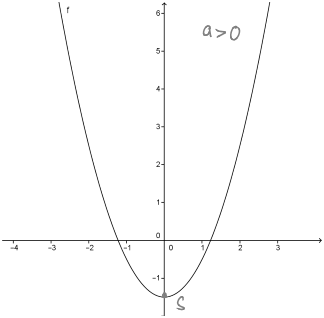
\includegraphics[width=\linewidth]{Bilder/101}
			\caption{}
		\end{minipage}
		\begin{minipage}{0.5\linewidth}
			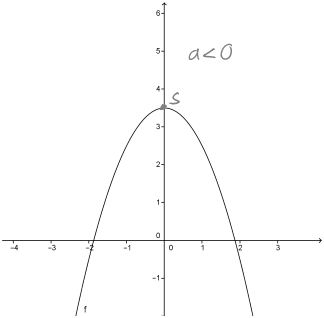
\includegraphics[width=\linewidth]{Bilder/102}
			\caption{}
		\end{minipage}
	\end{figure}
	
	$S(x_s,y_s)$ heißt \ul{Scheitel} der Parabel.
	
	Es gibt $x_s = -\dfrac{b}{2a}$\\
	$y_s=P(x_s)$ mit $P(x)=ax^2+bx+c$
	
	\ul{Normalform}:
	\redbox{$P(x)=ax^2+bx+c$}
	
	\ul{Scheitelform}:
	\redbox{$P(x)=a(x-x_s)^2+y_s$}\qquad $S(x_s,y_s)$ Scheitel
	
	\ul{Linearfaktorform}:
	\redbox{$P(x)=a(x-x_1)(x-x_2)$}
	
	mit $x_{1/2}=\dfrac{-b\pm\sqrt{D}}{2a}$
	
	\clearpage
	{\bf \item Quadratische Ungleichung}\\
	$ax^2+bx+c\le0\quad (a\ne0)$
	%bild 110
	\imgw{Bilder/103}{$D>0,\quad a<0$}{}{5cm}
	
	$\L=\{x\in\R\mid x\le x_1 \lor x\ge x_2\}\\
	=]-\infty;x_1]\cup[x_2;\infty[$
	
	\clearpage
	\paragraph{2. Methode:} Faktorisieren und Vorzeichentabelle (VZT)
	
	$ax^2+bx+c=a(x-x_1)(x-x_2)$\\
	mit $x_{1/2}=\dfrac{-b\pm\sqrt{D}}{2a}$ (falls $D\ge 0$)
	
	\greenbox{Für $D<0$} ist $ax^2+bx+c$ (über $\R$) unzerlegbar und hat für alle $x\in\R$ ein konstantes Vorzeichen (= Vorzeichen von $c$)
	
	\greenbox{Für $D=0$}: $x_1 = x_2$\\
	$ax^2+bx+c=a\underbrace{(x-x_1)^2}_{\ge0}$
	
	VZT:\\
	%bild 111
	\begin{tabular}{c|c|c|c}
		Faktoren & $-\infty<x<x_1$ & $x=x_1$ & $x_1<x<\infty$\\
		\hline
		$a$ & VZ & VZ & VZ \\
		$(x-x_1)^2$ & $+$ & $0$ & $+$ \\
		\hline
		$f(x)$ & VZ & $0$ & VZ \\
	\end{tabular}
	
	\greenbox{Für $D>0$}: $x_1 < x_2$\\
	$ax^2+bx+c=a(x-x_1)(x-x_2)$
	
	VZT:\\
	\begin{tabular}{c|c|c|c|c|c}
		Faktoren & $-\infty<x<x_1$ & $x=x_1$ & $x_1<x<x_2$ & $x=x_2$ & $x_2<x<\infty$\\
		\hline
		$a$ & VZ & VZ & VZ & VZ & VZ \\
		$x-x_1$ & $-$ & $0$ & $+$ & $+$ & $+$ \\
		$x-x_2$ & $-$ & $-$ & $-$ & $0$ & $+$ \\
		\hline
		$f(x)$ & VZ & $0$ & VZ & $0$ & VZ \\
	\end{tabular}
	
	\clearpage
	\Bsps
	\begin{enumerate}[1.]
		\item $-2x^2+4x-2\ge0$
		
		$D=16-4(-2)(-2) = 0$
		
		$x_1=x_2 = \dfrac{-b}{2a}= \dfrac{-4}{-4}= 1$
		
		$\Rightarrow -2x^2+4x-2=-2(x-1)^2$
		
		VZT:\\
		\begin{tabular}{c|c|c|c}
			Faktoren & $-\infty<x<1$ & $x=1$ & $1<x<\infty$\\
			\hline
			$-2$ & $-$ & $-$ & $-$ \\
			$(x-1)^2$ & $+$ & $0$ & $+$ \\
			\hline
			$f(x)$ & $-$ & $\red{\underbrace{\black{0}}_{\ge0}}$ & $-$ \\
		\end{tabular}
		
		$\Rightarrow \L=\{1\}$
		
		\item $-3x^2+6x-2\le0$
		
		$D=36-4(-3)(-2) = 12 > 0$
		
		$\Rightarrow x_1 < x_2$
		
		$x_{1/2} = \dfrac{-6\pm\sqrt{12}}{-6} = \dfrac{-6\pm2\sqrt{3}}{-6} = 1 \pm \frac{1}{3}\sqrt{3}$
		
		$\Rightarrow f(x) = -3(x - 1 + \frac{1}{3}\sqrt{3})(x - 1 - \frac{1}{3}\sqrt{3})$
		
		VZT:\\
		\begin{longtable}{c|c|c|c|c|c}
			Faktoren & \parbox{12ex}{$-\infty<x<1 - \frac{1}{3}\sqrt{3}$} & \parbox{8ex}{$x=1 - \frac{1}{3}\sqrt{3}$} & \parbox{12ex}{$1 - \frac{1}{3}\sqrt{3}<x<1 + \frac{1}{3}\sqrt{3}$} & \parbox{8ex}{$x=1 + \frac{1}{3}\sqrt{3}$} & \parbox{12ex}{$1 + \frac{1}{3}\sqrt{3}<x<\infty$}\\
			\hline
			$a$ & $-$ & $-$ & $-$ & $-$ & $-$ \\
			$x - 1 + \frac{1}{3}\sqrt{3}$ & $-$ & $0$ & $+$ & $+$ & $+$ \\
			$x - 1 - \frac{1}{3}\sqrt{3}$ & $-$ & $-$ & $-$ & $0$ & $+$ \\
			\hline
			$f(x)$ & $\red{\underbrace{\black{-}}_{\le0}}$ & $\red{\underbrace{\black{0}}_{\le0}}$ & $+$ & $\red{\underbrace{\black{0}}_{\le0}}$ & $\red{\underbrace{\black{-}}_{\le0}}$ \\
		\end{longtable}
		
		$\Rightarrow \L=]-\infty;1 - \frac{1}{3}\sqrt{3}] \cup [1 + \frac{1}{3}\sqrt{3};\infty[$
		
		\imgw{Bilder/104}{}{}{12cm}
		
		\item $-x^2+x-1>0$
		
		$D=1-4(-1)(-1) = -3 < 0$
		
		$\Rightarrow -x^2+x-1$ (über $\R$) unzerlegbar
		
		$\Rightarrow$ konstantes VZ\\
		$x=0$ eingesetzt $\Rightarrow -x^2+x-1<0$ für alle $x\in\R$
		
		$\Rightarrow \L=\emptyset$
	\end{enumerate}
	
	\clearpage
	\paragraph{3. Methode:} Quadratische Ergänzung und nach $x$ umstellen (direkte Methode)
	
	\Bsp $-3x^2+6x-2\le0$
	
	Quadratische Ergänzung
	
	\begin{align*}
	-3x^2+6x &= -3(x^2-2x+1^2-1^2)\\
	a^2-2ab+b^2 &= (a-b)^2\\
	&= -3((x-1)^2-1)\\
	&= -3(x-1)^2+3\\
	\Rightarrow -3x^2+6x-2 &= -3(x-1)^2+3-2\\
	&= -3(x-1)^2+1\\
	\end{align*}
	
	\begin{minipage}{0.5\linewidth}
		\begin{align*}
		-3x^2+6x-2 &\le 0\\
		\Leftrightarrow -3(x-1)^2+1 &\le 0 \mid -1\\
		-3(x-1)^2 &\le -1 \mid \colon (-3)\\
		\underbrace{(x-1)^2}_{\ge0} &\le \underbrace{\frac{1}{3}}_{\ge0} \mid \sqrt{\quad}\\
		\underbrace{|x-1|}_\text{Abstand zwischen $x$ und $1$} &\le \dfrac{1}{\sqrt{3}}\\
		\end{align*}
	\end{minipage}
	\begin{minipage}{0.5\linewidth}
		\begin{align*}
		\underbrace{x^2}_{\ge0} &= \underbrace{4}_{\ge0} \mid \sqrt{\quad}\\
		\sqrt{x^2} &= \sqrt{4}\\
		|x| &= 2\\
		x &= \pm 2\\
		\end{align*}
		
		\Allg \quad\\$|x-a|$ = Abstand von $x$ und $a$
	\end{minipage}
	
	$\Rightarrow \L=]-\infty;1 - \frac{1}{3}\sqrt{3}] \cup [1 + \frac{1}{3}\sqrt{3};\infty[$
	
	\imgw{Bilder/105}{}{}{8cm}
	
	\Bem
	\begin{enumerate}
		\item $|x-a| \le r\qquad (\Leftrightarrow a-r \le x \le a+r)$
		\imgw{Bilder/106}{}{}{7cm}
		\item $|x-a| \ge r\qquad (\Leftrightarrow x\le a-r \quad\lor\quad x \ge a+r)$
		\imgw{Bilder/107}{}{}{7cm}
	\end{enumerate}
	
\end{enumerate}

\subsubsection{Gleichung/Ungleichung höheren Grades $(n\ge 3)$}
\begin{enumerate}[A)]
	{\bf \item Gleichung vom Grad $n$}\\
	$\underbrace{a_nx^n+a_{n-1}x^{n-1}+\ldots+a_1x+a_0}_{P(x)\quad\text{Polynom vom Grad }n} = 0\qquad (a_n\ne0)$
	
	\Bem Für $n\ge5$ gibt es (prinzipiell) keine Lösungsformeln ($\Rightarrow$ numerische Verfahren)
	
	\paragraph{Spezialfall:} Nullstelle $x=x_0$ sei bekannt
	
	$\Rightarrow$ Polynomdivision $\underbrace{P(x)}_\text{\parbox{1cm}{Polynom vom Grad $n$}}:(x-x_0) = \underbrace{Q(x)}_\text{\parbox{1cm}{Polynom vom Grad $n-1$}}$ (mit Rest = 0)
	
	$\Rightarrow$ Faktorisierung $P(x)=(x-x_0)\cdot Q(x) \entspricht$ {\flqq Linearfaktor $(x-x_0)$ abspalten\frqq}
	
	Gilt wiederum $Q(x_0) = 0$, so kann mittels Polynomdivision wieder der Linearfaktor $(x-x_0)$ abgespalten werden.
	
	\greenframe{$Q(x)=(x-x_0)\cdot Q_2(x)$}
	
	$\Rightarrow$ \greenframe{$P(x)=(x-x_0)^2\cdot Q_2(x)$}
	
	Verfahren kann solange fortgesetzt werden, bis \redbox{$P(x)=(x-x_0)^m\cdot Q_m(x)$} mit $Q_m(x_0) \ne0$ gilt.\\
	Der Exponent $m$ heißt \ul{Vielfachheit} der Nullstelle $x_0$ von $P(x)$.
	
	\clearpage
	\Bsp $P(x)=x^3-4x^2+5x-2$ (alle Teiler von $-2:\pm1,\pm2$ als Nullstelle ausprobieren)
	
	$\Rightarrow$ z.B. $x=1$ ist Nullstelle
	
	\paragraph{Polynomdivision:}
	\imgw{Bilder/108}{Polynomdivision}{}{8cm}
	
	$\underbrace{x^3-4x^2+5x-2}_{P(x)}=(x-1)(\underbrace{x^2-3x+2}_{Q(x)})$
	
	\paragraph{Polynomdivision:}
	\imgw{Bilder/109}{Polynomdivision}{}{6cm}
	
	$\underbrace{x^3-4x^2+5x-2}_{P(x)}=(x-1)^2(\underbrace{x-2}_{Q_2(x)})$ (vollständige Faktorisierung)
	
	\begin{tabbing}
		Nullstellen von $P(x)$\=\qquad\=$x_1=1$\=\qquad\=(2-fach)\\
		\>\>$x_2=2$\>\>(1-fach)
	\end{tabbing}
	
	$x^3-4x^2+5x-2=(x-1)^2(x-2)$
	
	\Redbox{$x^3$: Leiterm, bestimmt das Verhalten im Unendlichen\\
		{\centering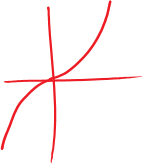
\includegraphics[width=2cm]{Bilder/110}}}
	
	\imgw{Bilder/111}{Graph/Skizze}{}{8cm}
	
	\begin{figure}[h!]
		{\bf m-fache Nullstelle $x_0$}
		
		\centering
		\begin{longtable}{c|c}
			m gerade & m ungerade\\
			\hline
			
\includegraphics[width=4cm]{Bilder/112} & 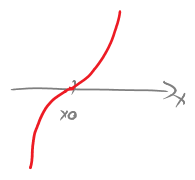
\includegraphics[width=4cm]{Bilder/114} \\
			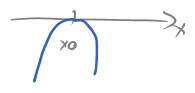
\includegraphics[width=4cm]{Bilder/113} & 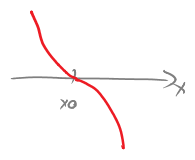
\includegraphics[width=4cm]{Bilder/115} \\
		\end{longtable}
		\caption{m-fache Nullstelle $x_0$}
	\end{figure}
	
	\Satz{{\bf vollständige Faktorisierung}\\
		\\
		Jedes reelle Polynom (vom Grad $\ge0$) ist darstellbar als Produkt von Faktoren der Form}

	\begin{enumerate}[1.]
		\item $a\quad(a\in\R)$ Konstante
		\item $(x-b)\quad(b\in\R)$ Linearfaktor
		\item $(x-c)^2+d^2\quad(c,d\in\R;\quad d\ne0)$ quadratischer Faktor, (über $\R$) unzerlegbar $D<0$
	\end{enumerate}
	
	\Bem Über den komplexen Zahlen $\C$ können die Faktoren $(x-c)^2+d^2$ in $2$ Linearfaktoren $(x-z_1)(x-z_2)$ zerlegt werden. $(z_1,z_2\in\C;\quad \ol{z_1}=z_2)$\\
	$z_{1/2}=c\pm \i d$
	
	{\bf \item Ungleichung vom Grad $n$}\\
	$\underbrace{a_nx^n+a_{n-1}x^{n-1}+\ldots+a_1x+a_0}_{P(x)\quad\text{Polynom vom Grad }n} \le 0\qquad (a_n\ne0)$
	
	\clearpage
	\Bsps
	\begin{enumerate}[1.]
		\item $-2x^2+8x-6\le0$\\
		Vollständige Faktorisierung: $ax^2+bx+c=a(x-x_1)(x-x_2)$
		
		$x_{1/2}=\dfrac{-b\pm\sqrt{D}}{2a}; \quad x_1=1,\quad x_2=3$
		
		$\Rightarrow -2x^2+8x-6 = -2(x-1)(x-3)$
		
		VZT:\\
		\begin{tabular}{c|c|c|c|c|c}
			Faktoren & $-\infty<x<1$ & $x=1$ & $1<x<3$ & $x=3$ & $3<x<\infty$\\
			\hline
			$-2$ & $-$ & $-$ & $-$ & $-$ & $-$ \\
			$x - 1$ & $-$ & $0$ & $+$ & $+$ & $+$ \\
			$x - 3$ & $-$ & $-$ & $-$ & $0$ & $+$ \\
			\hline
			$P(x)$ & $\red{\underbrace{\black{-}}_{\le0}}$ & $\red{\underbrace{\black{0}}_{\le0}}$ & $+$ & $\red{\underbrace{\black{0}}_{\le0}}$ & $\red{\underbrace{\black{-}}_{\le0}}$ \\
		\end{tabular}
		
		$\Rightarrow \L=]-\infty;1] \cup [3;\infty[$
		
		%bild 120
		\imgw{Bilder/116}{}{}{8cm}
		%bild 121
		\imgw{Bilder/117}{}{}{5cm}
		
		\clearpage
		\item $\underbrace{-x^3+3x2-3x+2}_{P(x)}>0$\\
		Vollständige Faktorisierung: Nullstellen erraten $\Rightarrow$ Teiler des \ul{konstanten Glieds} $\pm1,\pm2$
		
		$P(2)=0$
		
		Polynomdivision: $P(x):(x-2)$
		%bild 122
		\imgw{Bilder/118}{}{}{9cm}
		
		$\Rightarrow P(x) = -x^3+3x2-3x+2=(x-2)(\underbrace{-x^2+x-1}_\text{weiter zerlegbar?})$
		
		$D= 1^2 -4(-1)(-1)=1-4=-3 <0$\\
		$\Rightarrow$ (über $\R$) unzerlegbar
		
		VZT:\\
		\begin{tabular}{c|c|c|c}
			Faktoren & $-\infty<x<2$ & $x=2$ & $2<x<\infty$\\
			\hline
			$-2$ & $-$ & $-$ & $-$ \\
			$x - 2$ & $-$ & $0$ & $+$ \\
			$-x^2+x-1$ & $-$ & $-$ & $-$ \\
			\hline
			$P(x)$ & $\red{\underbrace{\black{+}}_{>0}}$ & $0$ & $-$ \\
		\end{tabular}
		
		$\Rightarrow \L=]-\infty;2[ = \{x<2\}$
		
		\clearpage
		\item $-4(x+2)^3x^5(x-1)^2(x-2)(\underbrace{2x^2-2x+3})\le0$\\
		$D=b^2-4ac < 0$\\
		$\Rightarrow$ (über $\R$) unzerlegbar
		
		$P(x) = -4(x+2)^3x^5(x-1)^2(x-2)(2x^2-2x+3)$ ist bereits vollständig faktorisiert.
		
		Nullstellen: $-2,0,1,2$
		
		VZT:
		
		\hspace{-65pt}
		\begin{tabular}{c|c|c|c|c|c|c|c|c|c}
			Faktoren & \parbox{38pt}{$-\infty<x<-2$} & $x=-2$ & \parbox{30pt}{$-2<x<0$} & $x=0$ & \parbox{30pt}{$0<x<1$} & $x=1$ & \parbox{30pt}{$1<x<2$} & $x=2$ & \parbox{35pt}{$2<x<\infty$}\\
			\hline
			$-4$ & $-$ & $-$ & $-$ & $-$ & $-$ & $-$ & $-$ & $-$ & $-$ \\
			$(x + 2)^3$ & $-$ & $0$ & $+$ & $+$ & $+$ & $+$ & $+$ & $+$ & $+$ \\
			$x^5$ & $-$ & $-$ & $-$ & $0$ & $+$ & $+$ & $+$ & $+$ & $+$ \\
			$(x - 1)^2$ & $+$ & $+$ & $+$ & $+$ & $+$ & $0$ & $+$ & $+$ & $+$ \\
			$x - 2$ & $-$ & $-$ & $-$ & $-$ & $-$ & $-$ & $-$ & $0$ & $+$ \\
			$2x^2-2x+3$ & $+$ & $+$ & $+$ & $+$ & $+$ & $+$ & $+$ & $+$ & $+$ \\
			\hline
			$P(x)$ & $+$ & $\red{\underbrace{\black{0}}_{\le0}}$ & $\red{\underbrace{\black{-}}_{\le0}}$ & $\red{\underbrace{\black{0}}_{\le0}}$ & $+$ & $\red{\underbrace{\black{0}}_{\le0}}$ & $+$ & $\red{\underbrace{\black{0}}_{\le0}}$ & $\red{\underbrace{\black{-}}_{\le0}}$ \\
		\end{tabular}
		
		$\Rightarrow \L=[-2;0] \cup \{1\} \cup [2;\infty[$
		%bild 123
		\imgw{Bilder/119}{}{}{8cm}
		
		\clearpage
		\item $x^4-(a+1)x^2+a<0 \qquad(a\in\R)$\\
		Vollständig Faktorisieren: $x^4-(a+1)x^2+a=0$ (biquadratische Gleichung)
		
		Substitution: $u=x^2$\\
		$u^2-(a+1)u+a=0$
		
		$D=(a+1)^2-4\cdot1\cdot a=(a+1)^2-4a=a^2+2a+1-4a=a^2-2a+1=(a-1)^2\ge0$
		
		$\Rightarrow u_{1/2}=\dfrac{a+1\pm\sqrt{(a-1)^2}}{2} = \dfrac{a+1\pm|a-1|}{2} = \dfrac{a+1\pm(a-1)}{2}$
		
		$\Rightarrow x_1=a,\quad x_2=1$
		
		$u^2-(a+1)u+a=0 = (u-a)(u-1)$
		
		Rücksubstitution: $x^2=u$\\
		$x^4-(a+1)x^2+a = (x^2-a)(x^2-1)= (x^2-a)(x-1)(x+1)$
		
		$(x^2-a)$ weiter zerlegbar? (ja, in Abhängigkeit von $a$)
		
		\ul{1. Fall}: $a<0$\\
		$\Rightarrow x^2-a$ (über $\R$) unzerlegbar (da $-a>0$)
		
		VZT:\\
		\begin{tabular}{c|c|c|c|c|c}
			Faktoren & $-\infty<x<-1$ & $x=-1$ & $-1<x<1$ & $x=1$ & $1<x<\infty$\\
			\hline
			$x^2-a$ & $+$ & $+$ & $+$ & $+$ & $+$ \\
			$x + 1$ & $-$ & $0$ & $+$ & $+$ & $+$ \\
			$x - 1$ & $-$ & $-$ & $-$ & $0$ & $+$ \\
			\hline
			$P(x)$ & $+$ & $0$ & $\red{\underbrace{\black{-}}_{<0}}$ & $0$ & $+$ \\
		\end{tabular}
		
		$\Rightarrow \L=]-1;1[ =\{-1<x<1\}$
		
		\ul{2. Fall}: $a=0$\\
		$\Rightarrow x^4-(a+1)x^2+a = x^2(x-1)(x+1)$ (vollständig faktorisiert)
		
		VZT:\\
		\begin{tabular}{c|c|c|c|c|c|c|c}
			Faktoren & \parbox{38pt}{$-\infty<x<-1$} & $x=-1$ & $-1<x<0$ & $x=0$ & $0<x<1$ & $x=1$ & \parbox{38pt}{$1<x<\infty$}\\
			\hline
			$x^2$ & $+$ & $+$ & $+$ & $+$ & $+$ & $+$ & $+$ \\
			$x + 1$ & $-$ & $-$ & $-$ & $-$ & $-$ & $0$ & $+$ \\
			$x - 1$ & $-$ & $-$ & $-$ & $0$ & $+$ & $+$ & $+$ \\
			\hline
			$P(x)$ & $+$ & $0$ & $\red{\underbrace{\black{-}}_{<0}}$ & $0$ & $\red{\underbrace{\black{-}}_{<0}}$ & $0$ & $+$ \\
		\end{tabular}
		
		$\Rightarrow \L=]-1;0[ \cup ]0;1[$
		
		\ul{3. Fall}: $a>0$\\
		$\Rightarrow x^4-(a+1)x^2+a = (x-\sqrt{a})(x+\sqrt{a})(x-1)(x+1)$ (vollständig faktorisiert)
		
		Nullstellen: $\pm1, \pm \sqrt{a}$
		%bild 124
		\imgw{Bilder/120}{}{}{8cm}
		
		\ul{$(0<)\sqrt{a}<1$}:
		
		VZT:
		
		\hspace{-75pt}
		\begin{tabular}{c|c|c|c|c|c|c|c|c|c}
			Faktoren & \parbox{38pt}{$-\infty<x<-1$} & $x=-1$ & \parbox{38pt}{$-1<x<-\sqrt{a}$} & $x=-\sqrt{a}$ & \parbox{38pt}{$-\sqrt{a}<x<\sqrt{a}$} & $x=\sqrt{a}$ & \parbox{38pt}{$\sqrt{a}<x<1$} & $x=1$ & \parbox{38pt}{$1<x<\infty$}\\
			\hline
			$x + 1$ & $-$ & $0$ & $+$ & $+$ & $+$ & $+$ & $+$ & $+$ & $+$ \\
			$x + \sqrt{a}$ & $-$ & $-$ & $-$ & $0$ & $+$ & $+$ & $+$ & $+$ & $+$ \\
			$x - \sqrt{a}$ & $-$ & $-$ & $-$ & $-$ & $-$ & $0$ & $+$ & $+$ & $+$ \\
			$x - 1$ & $-$ & $-$ & $-$ & $-$ & $-$ & $-$ & $-$ & $0$ & $+$ \\
			\hline
			$P(x)$ & $+$ & $0$ & $\red{\underbrace{\black{-}}_{<0}}$ & $0$ & $+$ & $0$ & $\red{\underbrace{\black{-}}_{<0}}$ & $0$ & $+$ \\
		\end{tabular}
		
		$\Rightarrow \L=]-1;-\sqrt{a}[ \cup ]\sqrt{a};1[$
		
		\ul{$\sqrt{a}=1$}:\\
		$\Rightarrow (x-1)^2(x+1)^2\ge0$
		
		$\Rightarrow \L=\emptyset$
		
		\ul{$\sqrt{a}>1$}:
		
		VZT:
		
		\hspace{-75pt}
		\begin{tabular}{c|c|c|c|c|c|c|c|c|c}
			Faktoren & \parbox{38pt}{$-\infty<x<-\sqrt{a}$} & $x=-\sqrt{a}$ & \parbox{38pt}{$-\sqrt{a}<x<-1$} & $x=-1$ & \parbox{38pt}{$-1<x<1$} & $x=1$ & \parbox{38pt}{$1<x<\sqrt{a}$} & $x=\sqrt{a}$ & \parbox{38pt}{$\sqrt{a}<x<\infty$}\\
			\hline
			$x + \sqrt{a}$ & $-$ & $0$ & $+$ & $+$ & $+$ & $+$ & $+$ & $+$ & $+$ \\
			$x + 1$ & $-$ & $-$ & $-$ & $0$ & $+$ & $+$ & $+$ & $+$ & $+$ \\
			$x - 1$ & $-$ & $-$ & $-$ & $-$ & $-$ & $0$ & $+$ & $+$ & $+$ \\
			$x - \sqrt{a}$ & $-$ & $-$ & $-$ & $-$ & $-$ & $-$ & $-$ & $0$ & $+$ \\
			\hline
			$P(x)$ & $+$ & $0$ & $\red{\underbrace{\black{-}}_{<0}}$ & $0$ & $+$ & $0$ & $\red{\underbrace{\black{-}}_{<0}}$ & $0$ & $+$ \\
		\end{tabular}
		
		$\Rightarrow \L=]-\sqrt{a};-1[ \cup ]1;\sqrt{a}[$
		
		%bild 125
		\imgw{Bilder/121}{Lösungsbaum}{}{13cm}
	\end{enumerate}
\end{enumerate}

\clearpage
\subsection{Zwei Unbestimmte $x_1,x_2$ ($x,y$)}
\subsubsection{Quadratische Gleichung/Ungleichung}
\begin{enumerate}[A)]
	{\bf \item Quadratische Gleichung}\\
	$a_1x_1^2+a_2x_1x_2+a_3x_2^2+a_4x_1+a_5x_2+a_6=0$
	
	Die Lösungsmengen (als Teilmengen der Ebene $\R^2$) heißen \ul{Kegelschnitte} (oder \ul{Quadriken}) zur Vereinfachung sei $a_2 = 0 \Rightarrow$ \ul{achsenparallele} Kegelschnitte
	
	Koordinaten $x,y$:\\
	\redbox{$Ax^2+By^2+Cx+Dy+E=0$} ($A,B,C,D,E \in\R;\quad \underbrace{A\ne0 \lor B\ne0}_{A^2+B^2\ne0}$)
	
	\paragraph{Klassifikation:}
	\begin{tabular}{ll}
		Kreis: & $A=B$ \\
		Ellipse: & $A\cdot B > 0 \land A\ne B$ \\
		Hyperbel: & $A\cdot B < 0$ \\
		Parabel: & $A=0\quad (\land B\ne0) \qquad\lor\qquad B=0\quad (\land A\ne0)$\\
	\end{tabular}
	
	\paragraph{Kreis} = Menge aller Punkte $P$, für die $\ol{PM} = r = \text{const}$ gilt.
	%bild 126
	\begin{figure}[h!]
		\begin{minipage}{5cm}
			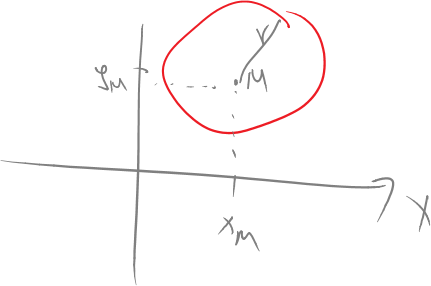
\includegraphics[width=\linewidth]{Bilder/122}
			\caption{}
		\end{minipage}
		\quad
		\begin{minipage}{\linewidth-5cm - 1em}
			Mittelpunkt $M(x_M;y_M)$\\
			Radius $r$
		\end{minipage}
	\end{figure}
	
	\ul{Hauptform} (allgemeine Kreisgleichung)
	\redbox{$(x-x_M)^2+(y-y_M)^2=r^2$} \qquad (implizite Gleichung)
	
	\paragraph{Ellipse}= Menge aller Punkte $P$, für die $\ol{PF_1}+\ol{PF_2}= 2a=\text{const}$ gilt.
	%bild 127
	\begin{figure}[h!]
		\begin{minipage}{8cm}
			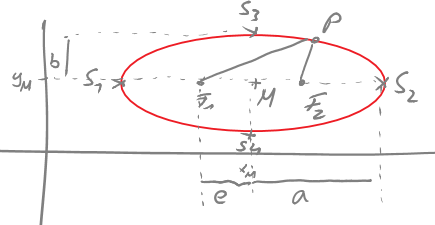
\includegraphics[width=\linewidth]{Bilder/123}
			\caption{}
		\end{minipage}
		\quad
		\begin{minipage}{\linewidth-8cm - 1em}
			Mittelpunkt $M(x_M;y_M)$\\
			$a:$ (große) Halbachse\\
			$b:$ (kleine) Halbachse\\
			Brennpunkte: $F_1,F_2$\\
			Brennweite: $e$ (Exzentrizität)\\
			Hauptscheitel $S_1,S_2$\\
			Nebenscheitel $S_3,S_4$
		\end{minipage}
	\end{figure}
	
	\redbox{$\underbrace{a^2}_\text{groß}=e^2+\underbrace{b^2}_\text{klein}$}
	
	\ul{Hauptform} (allgemeine Ellipsengleichung)
	\redbox{$\dfrac{(x-x_M)^2}{a^2}+\dfrac{(y-y_M)^2}{b^2}=1$} (implizite Gleichung)
	
	\paragraph{Hyperbel} = Menge aller Punkte P, für die $|\ol{PF_1}-\ol{PF_2}| = 2a = \text{const}$ gilt.
	%bild 128
	\begin{figure}[h!]
		\begin{minipage}{9cm}
			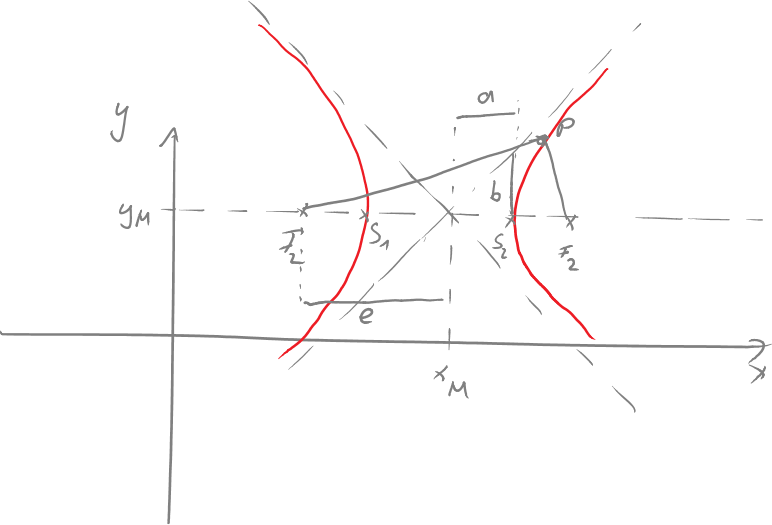
\includegraphics[width=\linewidth]{Bilder/124}
			\caption{}
		\end{minipage}
		\quad
		\begin{minipage}{\linewidth-9cm - 1em}
			Mittelpunkt $M(x_M;y_M)$\\
			$a:$ (große) reelle Halbachse\\
			$b:$ (kleine) imaginäre Halbachse\\
			Brennpunkte: $F_1,F_2$\\
			Brennweite: $e$ (Exzentrizität)\\
			Scheitel $S_1,S_2$
		\end{minipage}
	\end{figure}
	
	\redbox{$e^2=a^2+b^2$}
	
	\ul{Hauptform} (allgemeine Hyperbelgleichung)
	\redbox{$\dfrac{(x-x_M)^2}{a^2}-\dfrac{(y-y_M)^2}{b^2}=1$} (implizite Gleichung)
	
	zwei Asymptoten: \redbox{$y=y_M\pm\dfrac{b}{a}(x-x_M)$}\quad ($a,b > 0$)
	
	\paragraph{Parabel} = Menge aller Punkte $P$, für die $\ol{PF}=\ol{Pa}$ ($a$ = Gerade) gilt.
	%bild 129
	\begin{figure}[h!]
		\begin{minipage}{6cm}
			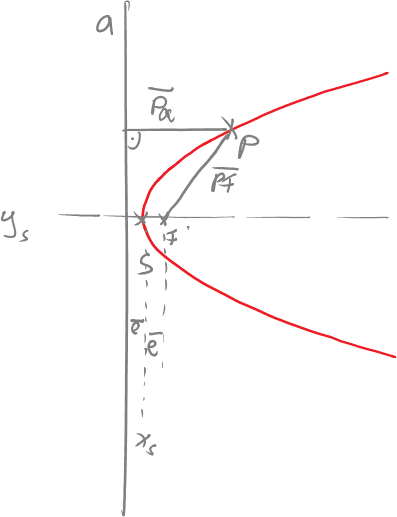
\includegraphics[width=\linewidth]{Bilder/125}
			\caption{}
		\end{minipage}
		\quad
		\begin{minipage}{\linewidth-6cm - 1em}
			Scheitel $S(x_S;y_S)$\\
			$|p|=$ Abstand Brennpunkt $\leftrightarrow$ Leitlinie\\
			$a$ Leitlinie\\
			$F$ Brennpunkt\\
			$e=\dfrac{|p|}{2}=\ol{FS}$ Brennweite
		\end{minipage}
	\end{figure}
	
	\ul{Hauptform} (allgemeine Parabelgleichung)
	\redbox{$(y-y_S)^2 = 2p(x-x_S)$} (implizite Gleichung)
	
	$p>0$ so ist Parabel nach rechts geöffnet\\
	$p<0$ so ist Parabel nach links geöffnet
	
	\clearpage
	\paragraph{Transformation:} $\red{Ax^2}+\blue{By^2}+\red{Cx}+\blue{Dy}+E=0 \longrightarrow$ Hauptform
	
	$\underbrace{\red{Ax^2}+\red{Cx}}_\text{\parbox{2cm}{\red{quadratische Ergänzung bezüglich $x$ (falls $C\ne0$)}}}+\underbrace{\blue{By^2}+\blue{Dy}}_\text{\parbox{2cm}{\blue{quadratische Ergänzung bezüglich $y$ (falls $D\ne0$)}}}+E=0$
	
	\gray{Wiederholung Quadratische Ergänzung:\\
	\vdots}

	\gray{\bf \item Quadratische Gleichung}\\
	\gray{\vdots}
\end{enumerate}

\clearpage
\subsubsection{Gleichung/Ungleichung höheren Grades $(n\ge 3)$}
Die Lösungsmengen der algebraischen Gleichung\\
$P(x,y)=0$\\
heißen \ul{algebraische Kurven}.

$P(x,y)=$ Polynom (multivariates)

\Bsp $P(x,y) = y^2-x^3-ax-b$, d.h. $y^2-x^3-ax-b=0 \Leftrightarrow y^2=x^3+ax+b$ (Lösung ist eine sogenannte \ul{elliptische Kurve})

%bild 130
\imgw{Bilder/126}{Addition auf elliptischen Kurven $P_1\oplus P_2 = Q$}{}{8cm}

($\Rightarrow$ Kryptographie!)

\clearpage
\section{Bruchgleichungen und Bruchungleichungen}
Unbestimmte tritt (bzw. treten) im Nenner von Bruchtermen auf.

\paragraph{Lösungsstrategie:}
\begin{enumerate}
	\item Gleichungen/Ungleichungen mit Hauptnenner (HN) multiplizieren ($\Rightarrow$ Fallunterscheidung! HN>0, HN<0 bei Ungleichungen)
	\item Nennerfreie Gleichung/Ungleichung lösen
	\item Probe (erforderlich, falls Grundmenge $\G$ nicht bestimmt ist)
\end{enumerate}

\gray{Wiederholung Bruchregeln\\
	\vdots}

\clearpage
\Bsps
\begin{enumerate}
	\item $\dfrac{2}{x^2} + \dfrac{3}{2x} = 0\qquad\G=\R\setminus\{0\}=\{x\ne0\}$
	
	\begin{tabular}{c|c}
		Nenner & EF (Erweiterungsfaktor) \\
		\hline
		$x^2$ & $2$ \\
		$2x$ & $x$ \\
		\hline
		HN=$2x^2$ & HN$\ne0$ auf $\G$ \\
	\end{tabular}
	
	\begin{align*}
	\dfrac{2}{x^2} + \dfrac{3}{2x} &= 0\\
	\Leftrightarrow\dfrac{4}{\text{HN}} + \dfrac{3x}{\text{HN}} &= 0\\
	\Leftrightarrow\dfrac{4+3x}{\text{HN}} &= 0 \mid\cdot \text{HN}(\ne0)\\
	\Leftrightarrow4+3x &= 0\\
	\Leftrightarrow x &= -\dfrac{4}{3} \in\G\\
	\end{align*}
	
	alternativ {\flqq Probe\frqq} durchführen
	
	\clearpage
	\item\label{b2} $\dfrac{x^2}{4x-8} = \dfrac{5-x^2}{x-2}\qquad\G=\R\setminus\{2\}=\{x\ne2\}$
	
	\begin{tabular}{c|c}
		Nenner & EF (Erweiterungsfaktor) \\
		\hline
		$4x-8 = 4(x-2)$ & $1$ \\
		$x-2$ & $4$ \\
		\hline
		HN=$4(x-2)$ & \\
	\end{tabular}
	
	%bild 131
	\begin{align*}
	\dfrac{x^2}{4x-8} &= \dfrac{5-x^2}{x-2}\\
	\Leftrightarrow\dfrac{x^2}{\text{HN}} &= \dfrac{4(5-x^2)}{\text{HN}}\mid\cdot \text{HN}(\ne0)\\
	\Leftrightarrow x^2 &= 4(5-x^2)\\
	\Leftrightarrow x^2 &= 20-4x^2\mid +4x^2\\
	\Leftrightarrow 5x^2 &= 20\\
	\Leftrightarrow x^2 &= 4\\
	\Leftrightarrow x &= \pm 2 & \G=\{x\ne2\}\\
	\end{align*}
	$x_1=2\not\in\G\Rightarrow$ keine Lösung der Bruchgleichung\\
	$x_2=-2\in\G\Rightarrow$ Lösung der Bruchgleichung
	
	$\Rightarrow \L=\{-2\}$
	
	\clearpage
	\item $\dfrac{x^2}{4x-8} < \dfrac{5-x^2}{x-2}\qquad\G=\R\setminus\{2\}=\{x\ne2\}$
	
	HN=$4(x-2)$ siehe \ref{b2})
	
	\begin{align*}
	\dfrac{x^2}{4x-8} &< \dfrac{5-x^2}{x-2}\\
	\Leftrightarrow\dfrac{x^2}{\text{HN}} &< \dfrac{4(5-x^2)}{\text{HN}}&(\text{HN}\ne0)\\
	\end{align*}
	
	\greenframe{1. Fall} HN$>0$, d.h. $4(x-2)>0\Leftrightarrow\grayframe{x>2}$
	
	\begin{align*}
	\dfrac{x^2}{\text{HN}} &< \dfrac{4(5-x^2)}{\text{HN}}\mid\cdot\text{HN}(>0)\\
	\Leftrightarrow x^2 &<4(5-x^2)\\
	\Leftrightarrow x^2 &<20-4x^2\mid+4x^2\\
	\Leftrightarrow 5x^2 &<20\mid\colon5\\
	\Leftrightarrow \underbrace{x^2}_{\ge0} &<\underbrace{4}_{\ge0}\mid\sqrt{\ }&\text{(streng monoton steigend auf }x\ge0)\\
	\Leftrightarrow \sqrt{x^2} &< \sqrt{4}\\
	\Leftrightarrow |x| &< 2\\
	\Leftrightarrow -2 < x &< 2\\
	\text{zudem gilt }\G &= \{x>2\}\\
	\end{align*}
	
	\begin{figure}[h!]
		\centering
		\begin{minipage}{0.4\linewidth-1em}
			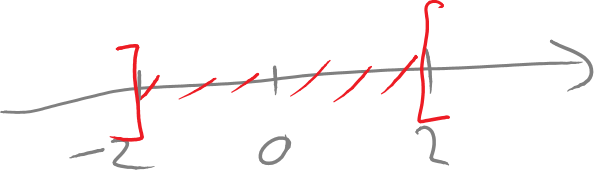
\includegraphics[width=\linewidth]{Bilder/127}
			\caption{$|x| < 2 \Leftrightarrow -2 < x < 2$}
		\end{minipage}
		\quad
		\begin{minipage}{0.4\linewidth-1em}
			\centering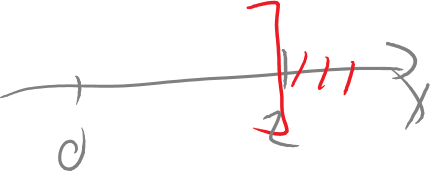
\includegraphics[width=0.8\linewidth]{Bilder/128}
			\caption{$\G=\{x>2\}$}
		\end{minipage}
	\end{figure}
	
	$\Rightarrow \L_1=\emptyset$
	
	\greenframe{2. Fall} HN$<0$, d.h. $4(x-2)>0\Leftrightarrow\grayframe{x<2}$
	
	\begin{align*}
	\dfrac{x^2}{\text{HN}} &< \dfrac{4(5-x^2)}{\text{HN}}\mid\cdot\text{HN}(<0)\\
	\Leftrightarrow x^2 &\redframe{>}4(5-x^2)\\
	\Leftrightarrow x^2 &>20-4x^2\mid+4x^2\\
	\Leftrightarrow 5x^2 &>20\mid\colon5\\
	\Leftrightarrow \underbrace{x^2}_{\ge0} &>\underbrace{4}_{\ge0}\mid\sqrt{\ }&\text{(streng monoton steigend auf }x\ge0)\\
	\Leftrightarrow \sqrt{x^2} &> \sqrt{4}\\
	\Leftrightarrow |x| &> 2\\
	\text{zudem gilt }\G &= \{x<2\}\\
	\end{align*}
	
	\begin{figure}[h!]
		\centering
		\begin{minipage}{0.4\linewidth-1em}
			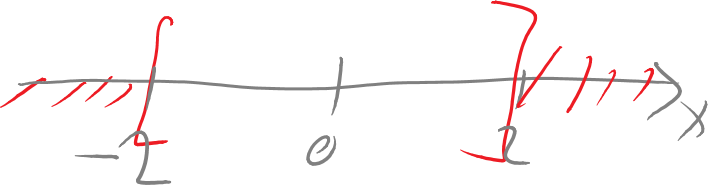
\includegraphics[width=\linewidth]{Bilder/129}
			\caption{$|x| > 2$}
		\end{minipage}
		\quad
		\begin{minipage}{0.4\linewidth-1em}
			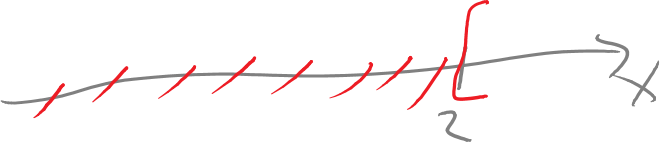
\includegraphics[width=\linewidth]{Bilder/130}
			\caption{$\G=\{x<2\}$}
		\end{minipage}
	\end{figure}
	
	$\Rightarrow \L_2=\{x<-2\}$
	
	\greenframe{insgesamt} $\Rightarrow \L=\L_1\cup\L_2=\{x<-2\}$
\end{enumerate}

\section{Wurzelgleichungen}
Unbestimmte steht (bzw. stehen) unter einer Wurzel (bzw. in einem Term mit echt rationalen Exponenten)

\paragraph{Lösungsstrategie:}
\begin{enumerate}
	\item\label{l1} Wurzel (bzw. Term mit rationalem Exponenten) isolieren
	\item\label{l2} Quadrieren (bzw. Potenzieren)
	\item Falls noch Wurzelterme auftreten wiederhole \ref*{l1}. und \ref*{l2}.
	\item Löse die wurzelfreie Gleichung
	\item Probe
\end{enumerate}

\Beachte Potenzieren mit geradzahligen Exponenten ist i.a. \ul{keine} Äquivalenzumformung.\\
$\Rightarrow$ zusätzliche (Schein-)Lösungen können auftreten\\
$\Rightarrow$ Probe notwendig

\clearpage
\Bsp $\sqrt{2x+8} - \sqrt{5+x} = 1$

$2x+8\ge0\Leftrightarrow x\ge -4\\
5+xx\ge0\Leftrightarrow x\ge -5$
%bild 130
\imgw{Bilder/131}{}{}{6cm}

$\Rightarrow \G=[-4;\infty[=\{x\ge -4\}$

\begin{align*}
\sqrt{2x+8} - \sqrt{5+x} &= 1\mid+\sqrt{5+x}\\
\Leftrightarrow \underbrace{\sqrt{2x+8}}_{\ge0} &= \underbrace{1 + \sqrt{5+x}}_{\ge0}\mid\square^2\\
\Leftrightarrow 2x+8 &= (1 + \sqrt{5+x})^2\\
\Leftrightarrow 2x+8 &= 1^2 + 2\sqrt{5+x}+5+x\\
\Leftrightarrow x+2 &= 2\sqrt{5+x}\mid:2\\
\Leftrightarrow \underbrace{\frac{1}{2}x+1}_\text{?} &= \underbrace{\sqrt{5+x}}_{\ge0}\mid\square^2\\
\red{\text{wurzelfreie Gleichung}}\Rightarrow (\frac{1}{2}x+1)^2 &= 5+x &\text{\ul{keine} Äquivlenzumformung, daher }\Rightarrow\\
\Leftrightarrow \frac{1}{4}x^2 + x + 1 &= 5+x \mid-5-x\\
\Leftrightarrow \frac{1}{4}x^2 -4 &= 0\\
\Leftrightarrow \frac{1}{4}x^2 &= 4\\
\end{align*}
\begin{align*}
\Leftrightarrow x^2 &= 16\\
\Leftrightarrow x &= \pm4 &\text{Lösung der wurzelfreien Gleichung}\\
\pm4\in\G\\
\end{align*}

%Randnotiz
\paragraph{Notiz:}
%Bild c=0 und b=0 ohne Formel auflösen
Wenn in der Form $ax^2+bx+c=0$ $c=0$ oder $b=0$ dann kann die Gleichung ohne Lösungsformel aufgelöst werden.

\paragraph{Probe:} \quad\\
\grayframe{$x=4$}: \ldots $1=1$ Ok\\
\grayframe{$x=-4$}: \ldots $-1=1$ Geht nicht

$\Rightarrow \L=\{4\}$

\clearpage
\section{Exponential- und Logarithmusgleichungen}
Unbestimmte steht (bzw. stehen) im Exponenten einer Potenz (Exponentialgleichung) bzw. im Argument eines Logarithmus (Logarithmusgleichung).

\paragraph{Lösungsstrategie:} Exponentialgleichungen
\begin{enumerate}
	\item\label{el1} Potenz(en) isolieren
	\item Logarithmieren (beide Seiten)
	\item Lösung bestimmen (auf $\G$ achten)
	\item (evtl.) Probe
\end{enumerate}

Ist bei \ref*{el1}. Isolierung nicht möglich $\Rightarrow$ Substitution

\gray{Wiederholung Potenzgesetze\\
	\vdots}

\gray{Wiederholung Logarithmusgesetze\\
	\vdots}

\clearpage
\Bsps Exponentialgleichung
\begin{enumerate}
	\item $5^x=12$
	\begin{align*}
	5^x&=12\mid \ln(\square)\\
	\Leftrightarrow \ln(5^x) &= \ln(12) &(\text{bzw. }\ln5^x = \ln12)\\
	\Leftrightarrow x\cdot\ln5 &= \ln12\\
	\Leftrightarrow x = \dfrac{\ln12}{\ln5}\\
	\end{align*}
	
	\item $\left(\dfrac{5}{2}\right)^{2x-1} = \dfrac{1}{4^x}$
	\begin{align*}
	\left(\dfrac{5}{2}\right)^{2x-1} &= \dfrac{1}{4^x}\\
	\Leftrightarrow \left(\dfrac{5}{2}\right)^{2x-1} &= 4^{-x}\mid\ln\square &\text{Potenzen isoliert}\\
	\Leftrightarrow \ln\left(\left(\dfrac{5}{2}\right)^{2x-1}\right) &= \ln\left(4^{-x}\right)\\
	\Leftrightarrow (2x-1)\ln\dfrac{5}{2} &= -x\ln4\\
	\Leftrightarrow 2x\ln\dfrac{5}{2}-\ln\dfrac{5}{2} &= -x\ln4\mid +x\ln4+\ln\dfrac{5}{2}\\
	\Leftrightarrow 2x\ln\dfrac{5}{2}+x\ln4 &= \ln\dfrac{5}{2}\\
	\Leftrightarrow x\left(2\ln\dfrac{5}{2}+\ln4\right) &= \ln\dfrac{5}{2}\\
	\Leftrightarrow x\left(\ln\dfrac{25}{4}+\ln4\right) &= \ln\dfrac{5}{2}\\
	\end{align*}
	\begin{align*}
	\Leftrightarrow x\left(\ln\dfrac{25\cdot 4}{4}\right) &= \ln\dfrac{5}{2}\\
	\Leftrightarrow x\ln25 &= \ln\dfrac{5}{2}\\
	\Leftrightarrow x &= \dfrac{\ln\dfrac{5}{2}}{\ln25}\\
	\end{align*}
	
	\item $5\cdot 3^{2x}=3^{x+3}-34$\\
	Potenzen können wegen Subtraktion (auf rechten Seite) \ul{nicht} isoliert werden.
	
	$\Rightarrow$ \ul{Substitution}: $u=3^x$
	
	$3^{2x}=(3^x)^2 = u^2\\
	3^{x+3} = 3^x\cdot3^3 = 27u$
	
	$\Rightarrow 5u^2=27u-34$
	
	$\Rightarrow$ Lösungsformel $u_1=2;\quad u_2=3{,}4$
	
	\ul{Rücksubstitution}:
	
	\grayframe{$u=2$}$(>0)$
	
	$u=3^x\\
	2=3^x\\
	\ln2=x\ln3\\
	x=\dfrac{\ln2}{\ln3}$
	
	\grayframe{$u_2=3{,}4$}
	
	$u=3^x\\
	3{,}4=3^x\\
	\ln3{,}4=x\ln3\\
	x=\dfrac{\ln3{,}4}{\ln3}$
	
	$\Rightarrow \L=\{\dfrac{\ln2}{\ln3};\dfrac{\ln3{,}4}{\ln3}\}$
\end{enumerate}

\clearpage
\paragraph{Lösungsstrategie:} Logarithmusgleichung
\begin{enumerate}
	\item Logarithmus(-men) isolieren ($\Rightarrow$ sonst Substitution)
	\item In den Exponenten heben (beide Seiten)
	\item Lösungen bestimmen (auf $\G$ achten)
	\item (evtl.) Probe
\end{enumerate}

\clearpage
\Bsps
\begin{enumerate}
	\item $\log_3(2x) = 2\qquad\G=\{x>0\}$
	\begin{align*}
	\log_3(2x) &= 2\mid3^\square &(\log\text{ bereits isoliert})\\
	\Leftrightarrow 3^{\log_3(2x)} &= 3^2\\
	\Leftrightarrow 2x &= 9\\
	\Leftrightarrow x &= \dfrac{9}{2}\\
	\end{align*}
	
	\paragraph{Probe:} \ldots 2 Ok
	
	$\Rightarrow \L=\{\frac{9}{2}\}$
	
	\item $\ln(2x+3)+\ln(1-x) = \ln(1-4x)\qquad\G=]-\frac{3}{2};\frac{1}{4}[$
	
	\begin{tabbing}
		$\G$ bestimmen: \=$2x+3>0\Leftrightarrow x>-\frac{3}{2}$\\
		\>$1-x>0\Leftrightarrow x<1$\\
		\>$1-4x>0\Leftrightarrow x<\frac{1}{4}$\\
	\end{tabbing}
	%bild 131
	\imgw{Bilder/132}{}{}{6cm}
	
	\begin{align*}
	\ln(2x+3)+\ln(1-x) &= \ln(1-4x)\\
	\Leftrightarrow \ln[(2x+3)(1-x)] &= \ln(1-4x)\mid e^\square\\
	\Leftrightarrow (2x+3)(1-x) &= 1-4x\\
	\Leftrightarrow 2x^2-3x-2 &= 0\\
	x_{1/2} &= \dfrac{3\pm5}{4}\\
	\Rightarrow x_1 &= 2\not\in\G\\
	x_2 &= -\frac{1}{2}\in\G\\
	\end{align*}
	
	$\Rightarrow \L=\{-\frac{1}{2}\}$
\end{enumerate}

\clearpage
\section{Goniometrische Gleichungen}
Die Unbestimmte(n) tritt (treten) im Argument einer Winkelfunktion (trigonometrischen Funktion) auf.

\gray{Wiederholung Winkelfunktionen\\
	\vdots}

\paragraph{Es gilt:} \quad\\
$\cos\alpha=\sin\beta = \sin(90\degree - \alpha)\\
\sin\alpha=\cos\beta = \cos(90\degree - \alpha)\\
\tan\alpha=\dfrac{\sin\alpha}{\cos\alpha} = \dfrac{\cos\beta}{\sin\beta} =\cot\beta = \cot(90\degree - \alpha) = \dfrac{1}{\tan(90\degree - \alpha)}$

\paragraph{Gleichungen der Form $\sin x = a, \cos x = a$:}
\Beachte dass $-1\le\sin x\le 1$ und $-1\le\cos x\le 1$ gilt.

D.h. Gleichungen der Form $\sin x = a$ bzw. $\cos x = a$ haben für $|a|>1$ \ul{keine} Lösungen.

\greenframe{$a = 0$:}\\
$\sin x = 0 \Leftrightarrow x =0+k\pi = k\pi \qquad (k\in\Z)$\\
$\cos x = 0 \Leftrightarrow x =\frac{\pi}{2}+k\pi \qquad (k\in\Z)$

\greenframe{$a = 1$:}\\
$\sin x = 1 \Leftrightarrow x =\frac{\pi}{2}+k2\pi \qquad (k\in\Z)$\\
$\cos x = 1 \Leftrightarrow x =0+k2\pi = k2\pi \qquad (k\in\Z)$

\greenframe{$a = -1$:}\\
$\sin x = -1 \Leftrightarrow x =\frac{3}{2}\pi+k2\pi \qquad (k\in\Z)$\\
$\cos x = -1 \Leftrightarrow x =\pi+k2\pi \qquad (k\in\Z)$

\greenframe{$0<a<1$:}\\
$\sin x = a$

Lösung im I. Quadrant\\
$x_1 = \arcsin a = \sin^{-1}a>0$\\
Lösung im II. Quadrant\\
$x_2 = \pi - x_1$\\
allgemeine Lösungen:\\
$x_1+k2\pi\\
x_2+k2\pi \qquad (k\in\Z)$

$\cos x = a$

Lösung im I. Quadrant\\
$x_1 = \arccos a = \cos^{-1}a>0$\\
Lösung im IV. Quadrant\\
$x_2 = 2\pi - x_1$\\
allgemeine Lösungen:\\
$x_1+k2\pi\\
x_2+k2\pi \qquad (k\in\Z)$

\greenframe{$-1<a<0$:}\\
$\sin x = a$

Lösung im III. Quadrant\\
$x_1 = \arcsin a = \sin^{-1}a<0$\\
Lösung im IV. Quadrant\\
$x_2 = \pi - x_1$\\
allgemeine Lösungen:\\
$x_1+k2\pi\\
x_2+k2\pi \qquad (k\in\Z)$

$\cos x = a$

Lösung im II. Quadrant\\
$x_1 = \arccos a = \cos^{-1}a>0$\\
Lösung im III. Quadrant\\
$x_2 = 2\pi - x_1$\\
allgemeine Lösungen:\\
$x_1+k2\pi\\
x_2+k2\pi \qquad (k\in\Z)$

\Beachte \quad\\
$0\le\arccos a\le\pi$ (I. oder II. Quadrant)\\
$-\frac{\pi}{2}\le\arccos a\le\frac{\pi}{2}$ (I. oder IV. Quadrant)

\paragraph{Goniometrische Beziehungen:}\quad

\ul{Additionstheoreme:}\\
$\sin(x_1\pm x_2) = \sin x_1\cos x_2 \pm \cos x_1\sin x_2\\
\cos(x_1\pm x_2) = \cos x_1\cos x_2 \mp \sin x_1\sin x_2$

\ul{Doppelter Winkel:}\\
$\sin2x = 2\sin x\cos x\\
\cos2x = \cos^2 x-sin^2x = 1-2sin^2x = 2cos^2x-1$

\ul{Summen und Differenzen:}\\
$\sin x_1 \pm \sin x_2 = 2\sin\dfrac{x_1\pm x_2}{2}\cos\dfrac{x_1\mp x_2}{2}\\
\cos x_1 + \cos x_2 = 2\cos\dfrac{x_1+x_2}{2}\cos\dfrac{x_1-x_2}{2}\\
\cos x_1 - \cos x_2 = -2\sin\dfrac{x_1+x_2}{2}\sin\dfrac{x_1-x_2}{2}$

\ul{Trigonometrischer Pythagoras:}\\
$\sin^2x + \cos^2x = 1$

\Bsps Goniometrische Gleichungen
\begin{enumerate}
	\item $\sin x = \frac{1}{2}\qquad \G=\R$
	
	Lösung im\\
	I. Quadranten $x_1=\arcsin\frac{1}{2} = \frac{\pi}{6}$\\
	II. Quadranten $x_2=\pi - x_1 = \pi - \frac{\pi}{6} = \frac{5}{6}\pi$\\
	allgemeine Lösungen:\\
	$x_1 = \frac{\pi}{6} + k2\pi\\
	x_2 = \frac{5}{6}\pi + k2\pi \qquad (k\in\Z)$
	
	\item $\sin2x=sin x \qquad \G=[0;2\pi[$
	\begin{align*}
	\underbrace{\sin2x}_{2\sin x\cos x} &= sin x\\
	\Leftrightarrow 2\sin x\cos x &= sin x\mid-\sin x\\
	\Leftrightarrow 2\sin x\cos x -\sin x &= 0\\
	\Leftrightarrow \sin x(2\cos x -1) &= 0\\
	\Leftrightarrow \sin x = 0 &\lor \underbrace{2\cos x -1 = 0}_{\cos x=\frac{1}{2}}\\
	\end{align*}
	
	\begin{align*}
	\sin x = 0 &\Leftrightarrow x=0 \lor x = \pi\\
	\cos x = \frac{1}{2} &\Leftrightarrow x=\frac{\pi}{3} \lor x = \frac{5}{3}\pi\\
	\end{align*}
	
	$\Rightarrow \L = \{0;\frac{\pi}{3};\pi;\frac{5}{3}\pi\}$
	
	\item $2\cos^2x = 1-\sin x \qquad \G=[0;2\pi[$
	\begin{align*}
	2\cos^2x &= 1-\sin x\\
	\Leftrightarrow 2(1-\sin^2x) &= 1-sin x\mid u = \sin x\\
	\Leftrightarrow 2(1-u^2) &= 1-u\\
	\Leftrightarrow 2(1-u)(1+u)-(1-u) &= 0\\
	\Leftrightarrow (1-u)(2(1+u)-1) &= 0\\
	\Leftrightarrow (1-u)(1+2u) &= 0\\
	\Leftrightarrow u= 1 &\lor u=-\frac{1}{2}\\
	\end{align*}
	
	\greenframe{$\sin x = u$}
	\grayframe{$u=1:$} $\sin x = 1 \Leftrightarrow x = \frac{\pi}{2}$\\
	\grayframe{$u=1:$} $\sin x = -\frac{1}{2} \Leftrightarrow x = \frac{11}{6}\pi \lor x = \frac{7}{6}\pi$\\
	
	$\Rightarrow \L = \{\frac{\pi}{2};\frac{11}{6}\pi;\frac{7}{6}\pi\}$
	
	%HÜ
	\item $\sqrt{2}\sin^2(2x)-\sin(2x) = 0 \qquad \G=[0;2\pi[$
	\item $\cos^4x-3\cos^2x\sin2x = 0 \qquad \G=[0;2\pi[$
\end{enumerate}

\section{Das Newton-Raphson-Verfahren}
Für viele Gleichungen ist es oftmals unmöglich eine exakte Lösung zu bestimmen $\Rightarrow$ Näherungslösungen (approximative Lösungen)!

\Bsp
%bild 140
\imgw{Bilder/133}{}{}{7cm}

Gesucht ist eine Lösung der Gleichung $f(x) = 0$

Starte mit beliebigem Punkt $x_0$
\begin{itemize}
	\item Konstruiere die Tangente an $G_f$ durch $P_0(x_0;\underbrace{y_0}_{f(x_0)})$\\
	Tangentengleichung $y = f'(x_0)(x-x_0)+f(x_0)$
	
	\item diese schneidet bei $x=x_1$ die $x$-Achse
	\begin{align*}
	0 &= f'(x_0)(x-x_0)+f(x_0)
	\Leftrightarrow x_1 &= x_0 - \dfrac{f(x_0)}{f'(x_0)}
	\end{align*}
	
	\item Wiederholt man die Konstruktion, so erhält man eine Folge $x_0, x_1, x_2, x_3, \ldots$ durch\\
	\redbox{$x_{n+1}=x_n-\dfrac{f(x_n)}{f'(x_n)}$} \qquad $(n = 0, 1, 2, \ldots)$
\end{itemize}

\Greenbox{Gilt für den Startwert $x_0$ die sogenannte \ul{Lipschitz-Bedingung}\\
$\left|\dfrac{f(x_0)\cdot f''(x_0)}{(f'(x_0))^2}\right| < 1$, (hinreichendes Konvergenzkriterium)\\
so konvergiert die Folge $x_0, x_1, x_2, x_3, \ldots$ gegen eine Nullstelle von $f(x)$.}

\cleardoublepage
\part{Analysis einer Veränderlichen}
\chapter{Folgen und Reihen}
\section{Grundbegriffe}
\Def Eine reelle (bzw. komplexe) \ul{Folge} ist eine Abbildung $\No\to\R$ (bzw. $\No\to\C$), $n\mapsto a_n$ (bzw. $n\mapsto z_n$); für Folge schreibt man auch $(a_n)_{n\in\No}$ (bzw. $(z_n)_{n\in\No}$) oder einfach nur $(a_n)$ (bzw. $(z_n)$).

\Bsp
\begin{enumerate}
	\item $a_n = 2n \quad (n\ge0)\quad(a_n) = (0,2,4,6,8,\ldots)$
	\item $a_n = n^2 \quad (n\ge0)\quad(a_n) = (0,1,4,9,\ldots)$
	\item Rekursive Definiton\\
	$a_0 = 1, a_1 = 4, a_2 = 10\\
	a_n = \frac{1}{2}(a_{n-3}+a_{n-2}-2a_{n-1}) \quad (n\ge3)$
	
	$a_3 = \frac{1}{2}(a_0+a_1-2a_2)= \ldots = -7{,}5$
	$a_4 = \frac{1}{2}(a_1+a_2-2a_3)= \ldots = 14{,}5$
\end{enumerate}

\Def Sind $(a_n),(b_n)$ Folgen und $\alpha\in\R$ (bzw. $\alpha\in\C$), so definiert man
\begin{enumerate}[a)]
	\item $(a_n)\pm(b_n) = (a_n\pm b_n)$
	\item $(a_n)\cdot(b_n) = (a_n\cdot b_n)$
	\item $(a_n)\colon(b_n) = (a_n\colon b_n)$
	\item $\alpha\cdot(a_n) = (\alpha\cdot a_n)$
\end{enumerate}

\Def Eine unendliche, reelle (bzw. komplexe) \ul{Reihe} ist ein formaler Ausdruck der Form\\
\redbox{$\sum\limits_{k=0}^{\infty}a_k = a_0+a_1+a_2+\ldots$}\\
wobei $(a_k)$ eine Folge ist.

\Bsp
\begin{enumerate}
	\item $\sum\limits_{k=0}^{\infty}k = 0+1+2+\ldots$
	\item $\sum\limits_{k=0}^{\infty}q^k = q^0+q^1+q^2+\ldots$
\end{enumerate}

\Def Sind $\sum\limits_{k=0}^{\infty}a_k$ und $\sum\limits_{k=0}^{\infty}b_k$ Reihen, $\alpha\in\R$, so definiert man:
\begin{enumerate}[a)]
	\item $\sum\limits_{k=0}^{\infty}a_k\pm \sum\limits_{k=0}^{\infty}b_k = \sum\limits_{k=0}^{\infty}(a_k\pm b_k)$
	\item\label{b} $\sum\limits_{k=0}^{\infty}a_k\cdot \sum\limits_{k=0}^{\infty}b_k = \sum\limits_{k=0}^{\infty}c_k$\\
	mit $c_k = \sum\limits_{m=0}^{k}a_m\cdot b_{k-m}$ (Cauchy-Produkt)
	\item $\alpha\cdot \left(\sum\limits_{k=0}^{\infty}a_k\right) = \sum\limits_{k=0}^{\infty}\alpha\cdot a_k$
\end{enumerate}

\Bem zu \ref*{b}) Cauchy-Produkt\\
$(a_0+a_1+a_2+a_3+\ldots)\cdot(b_0+b_1+b_2+b_3+\ldots)$

\begin{tabular}{c|c|c|c|c|c}
	& $b_0$ & $b_1$ & $b_2$ & $b_3$ & $\ldots$ \\
	\hline
	$a_0$ & \red{$a_0b_0$} & \blue{$a_0b_1$} & \green{$a_0b_2$} & \gray{$a_0b_3$} & $\ldots$ \\
	\hline
	$a_1$ & \blue{$a_1b_0$} & \green{$a_1b_1$} & \gray{$a_1b_2$} & $a_1b_3$ & $\ldots$ \\
	\hline
	$a_2$ & \green{$a_2b_0$} & \gray{$a_2b_1$} & $a_2b_2$ & $a_2b_3$ & $\ldots$ \\
	\hline
	$a_3$ & \gray{$a_3b_0$} & $a_3b_1$ & $a_3b_2$ & $a_3b_3$ & $\ldots$ \\
	%Diagonal
\end{tabular}

$\red{c_0} = \sum\limits_{m=0}^{0}a_mb_{0-m} = a_0b_0$\\
$\blue{c_1} = \sum\limits_{m=0}^{1}a_mb_{1-m} = a_0b_1+a_1b_0$\\
$\green{c_2} = \sum\limits_{m=0}^{2}a_mb_{2-m} = a_0b_2+a_1b_1+a_2b_0$\\
$\gray{c_3} = \sum\limits_{m=0}^{3}a_mb_{3-m} = a_0b_3+a_1b_2+a_2b_1+a_3b_0$\\

\clearpage
\section{Grenzwerte und Konvergenzkriterien}
\Def
\begin{enumerate}
	\item Eine (reelle) \ul{Folge} $(a_n)$ heißt \ul{Konvergent}, wenn es ein $a\in\R$, so dass gilt:\\
	\redbox{Zu jedem $\epsilon>0$ existiert ein $n_0\in\N$, so dass $|a_n-a|<\epsilon$ für alle $n\ge n_0$}\\
	wir schreiben dann\\
	\redbox{$\lim\limits_{n\to\infty}a_n = a$} \quad (bzw. $a_n\to a$ für $n\to\infty$)\\
	und nennen $a$ den \ul{Grenzwert} der Folge $(a_n)$; ist $a_n$ nicht konvergent, so heißt die Folge \ul{divergent}.
	%bild 150
	\imgw{Bilder/134}{}{}{13cm}
	
	\clearpage
	$\lim\limits_{n\to\infty}a_n=a$ bedeutet, dass es zu jeder noch so kleinen $\epsilon$-Umgebung $U_\epsilon(a)$ stets eine Schranke $n_o\in\N$ gibt, so dass alle $a_n$ mit $n\ge n_0$ in $U_\epsilon(a)$ liegen.
	
	Analog definiert man Konvergenz auch für \ul{komplexe Folgen} $(z_n)$; hierbei ist $|z_n-z|$ der Betrag für komplexe Zahl. Geometrisch ist $|z_n-z|$ der Abstand von $z_n$ zu $z$ in der Gaußschen Zahlenebene.
	
	\item Eine Folge $(a_n)$ heißt \ul{bestimmt divergent} mit \ul{uneigentlichem Grenzwert} $\pm\infty$, wenn es zu jedem $M\in\R$ ein $n_0\in\N$ gibt mit\\
	\redbox{$a_n>M$ für alle $n\ge n_0$}\quad(bzw. $a_n < M$ für alle $n\ge n_0$)\\
	wir schreiben dann\\
	\redbox{$\lim\limits_{n\to\infty}a_n=\pm\infty$}\\
	ansonsten heißt $(a_n)$ \ul{unbestimmt divergent}.
	%bild 151
	\imgw{Bilder/135}{}{}{0.8\linewidth}
	
	\Bem Eine komplexe Folge $(z_n), z_n = a_n +\i b_n$ ist genau dann konvergent, wenn Realteil $(a_n)$ und Imaginärteil $(b_nj)$ konvergente Folgen sind; dabei gilt\\
	\redframe{$\lim\limits_{n\to\infty}z_n=\lim\limits_{n\to\infty}a_n+\i b_n=a+\i b$} mit \redframe{$\lim\limits_{n\to\infty}a_n=a,\lim\limits_{n\to\infty}b_n=b$}
	
	\begin{enumerate}
		\item $\lim\limits_{n\to\infty}(1+\frac{1}{n})^n=e$ (Eulersche Zahl $e=2,71\ldots$)\\
		bzw. $\lim\limits_{n\to\infty}(1+\frac{x}{n})^n=e^x$ (konvergent)
		
		$|a_n-e^x|<10^{-8}$ maximaler Fehler\\
		$\Rightarrow n\ge n_0$
		
		\item $\lim\limits_{n\to\infty}2^n=\infty$ (bestimmt divergent)
		\item $\lim\limits_{n\to\infty}(\frac{1}{2})^n=0$ (konvergent)
		\item $\lim\limits_{n\to\infty}\sqrt[n]{a}=1 \qquad (a>0)$
	\end{enumerate}
\end{enumerate}

\subsection{Rechenregeln für Grenzwerte}
$(a_n),(b_n)$ Folgen mit $\lim\limits_{n\to\infty} a_n = a,\lim\limits_{n\to\infty} b_n = b$
\begin{enumerate}
	\item $\lim\limits_{n\to\infty} a_n\pm b_n = a\pm b$
	\item $\lim\limits_{n\to\infty} a_n\cdot b_n = a\cdot b$
	\item Falls $b\ne0$ und $b_n\ne0$ gilt $\lim\limits_{n\to\infty} \dfrac{a_n}{b_n} = \dfrac{a}{b}$
	\item $\lim\limits_{n\to\infty} \alpha\cdot a_n = \alpha\cdot a \qquad (\alpha\in\R)$
\end{enumerate}

\paragraph{Sandwich-Lemma:} sind $(a_n),(b_n),(c_n)$ Folgen und gilt
\begin{enumerate}
	\item $a_n\le b_n\le c_n$ {\flqq Sandwich\frqq}
	\item $\lim\limits_{n\to\infty} a_n =\lim\limits_{n\to\infty} c_n$
\end{enumerate}
Dann ist $(b_n)$ konvergent und es gilt \greenbox{$\lim\limits_{n\to\infty} b_n = \lim\limits_{n\to\infty} a_n = \lim\limits_{n\to\infty} c_n$}

\Bsp $b_n = \dfrac{\sin(n)}{n}\qquad (n>0)$

Es gilt:
\begin{align*}
-1\le\sin(n) &\le1\mid\colon n\\
\Leftrightarrow \underbrace{-\frac{1}{n}}_{a_n\to0}\le\underbrace{\dfrac{\sin(n)}{n}}_{b_n} &\le\underbrace{\frac{1}{n}}_{c_n\to0}\\
\end{align*}

$\Rightarrow$ Sandwich-Lemma $b_n = \dfrac{\sin(n)}{n}$ ist konvergent und $\lim\limits_{n\to\infty}\dfrac{\sin(n)}{n} = 0$

\Def
\begin{enumerate}[a)]
	\item Eine (unendliche) Reihe $\sum\limits_{k=0}^{\infty} a_n$ heißt \ul{konverget}, wenn es ein $a\in\R$ gibt, so dass Folge $(s_n)$ der \ul{Partialsummen}\\
	$s_n = \sum\limits_{k=0}^{n}a_k$\\
	gegen $a$ konvergiert, d.h. $a=\lim\limits_{n\to\infty}s_n = \lim\limits_{n\to\infty}\sum\limits_{k=0}^{n}a_k$, wir schreiben dann\\
	\redbox{$\sum\limits_{k=0}^{\infty} a_k = a$}\\
	und nennen $a$ den \ul{Grenzwert} der Reihe; ist die Reihe nicht konvergent, so heißt sie \ul{divergent}.
	
	\item $\sum\limits_{k=0}^{\infty}a_k$ heißt \ul{absolut konvergent}, wenn $\sum\limits_{k=0}^{\infty}|a_k|$ konvergent ist.
	
	\item $\sum\limits_{k=0}^{\infty}a_k$ heißt \ul{bestimmt divergent}, wenn die Folge $s_n = \sum\limits_{k=0}^{n}a_k$ der Partialsummen bestimmt divergent ist; wir schreiben dann\\
	\redbox{$\sum\limits_{k=0}^{\infty}a_k = \pm\infty$}\\
	ansonsten heißt die Reihe \ul{unbestimmt divergent}; $\pm\infty$ heißt \ul{uneigentlicher Grenzwert}.
\end{enumerate}

\Bsp
\begin{enumerate}
	\item $\sum\limits_{k=0}^{\infty}q^k=q^0+q^1+q^2+\ldots = \dfrac{1}{1-q}\qquad(0\le q<1)$ (geometrische Reihe)
	\item $\sum\limits_{k=1}^{\infty}\dfrac{1}{k^2} = \dfrac{\pi^2}{6}$
	\item $\sum\limits_{k=1}^{\infty}\dfrac{1}{k} = \infty$ (harmonische Reihe)
	\item $\sum\limits_{k=1}^{\infty}\dfrac{1}{k(k+1)} = 1$
\end{enumerate}

\Bem Eine absolut konvergente Reihe ist auch konvergent (absolut konvergent $\Rightarrow$ konvergent). Die Umkehrung gilt i.a. nicht.

\subsection{Konvergenzkriterien für Reihen}
hinreichende Kriterien

\begin{enumerate}
	\item Quotientenkriterium (D'Almbert)\\
	Gilt $\lim\limits_{k\to\infty}\left|\dfrac{a_{k+1}}{a_k}\right| = q\left\{\begin{array}{c}{<1}\\{>1}\end{array}\right\}$, so ist $\sum\limits_{k=0}^{\infty}a_k\left\{\begin{array}{c}\text{konvergent}\\\text{divergent}\end{array}\right\}$.
	
	\item Wurzelkriterium (Cauchy)\\
	Gilt $\lim\limits_{k\to\infty}\sqrt[k]{|a_k|} = q\left\{\begin{array}{c}{<1}\\{>1}\end{array}\right\}$, so ist $\sum\limits_{k=0}^{\infty}a_k\left\{\begin{array}{c}\text{konvergent}\\\text{divergent}\end{array}\right\}$.
	
	\item Majorantenkriterium 
	
	Ist $\sum\limits_{k=0}^{\infty}a_k$ konvergent und $|b_k|\le a_k$ für alle $k\ge N$, so ist auch $\sum\limits_{k=0}^{\infty}b_k$ konvergent.
	
	Ebenso gilt: Ist $\sum\limits_{k=0}^{\infty}a_k$ divergent und gilt $b_k\ge a_k$ für alle $k\ge N$, so ist auch $\sum\limits_{k=0}^{\infty}b_k$ divergent.
	
	\item Kriterium für alternierende Reihen (Leibniz)
	
	Ist $(a_n)$ eine monoton fallende Folge, d.h. $a_0\ge a_1\ge a_2\ge \ldots$ mit $\lim\limits_{k\to\infty}a_k = 0$, so konvergiert die Reihe $\sum\limits_{k=0}^{\infty}(-1)^ka_k$.
\end{enumerate}

\Bem Notwendiges Kriterium für Konvergenz (Bedingung)

Ist die Reihe $\sum\limits_{k=0}^{\infty}a_k$ konvergent, so ist $(a_k)$ eine sogenannte \ul{Nullfolge}, d.h. $\lim\limits_{k\to\infty}a_k = 0$.

\paragraph{Implikation} $A\imp B$ {\flqq aus $A$ folgt $B$\frqq}, {\flqq $A$ impliziert $B$\frqq}\\
Die Gültigkeit der Bedingung $A$ ist \ul{hinreichend} für die Gültigkeit von $B$\\
d.h. $A$ ist eine \ul{hinreichende} Bedingung/Kriterium für $B$.

Die Gültigkeit der Bedingung $B$ ist \ul{notwendig} für die Gültigkeit von $A$\\
d.h. $B$ ist eine \ul{notwendige} Bedingung/Kriterium für $A$.

{\flqq Reihe $\sum\limits_{k=0}^{\infty}a_k$ konvergiert\frqq}$\imp${\flqq $(a_k)$ ist Nullfolge\frqq}

\subsubsection{Rechenregeln für konvergente Reihen}
Es seien $\sum\limits_{k=0}^{\infty}a_k = a$ und $\sum\limits_{k=0}^{\infty}b_k = b$ konvergente Reihen, $\alpha\in\R$.

Dann sind auch die Reihen $\sum\limits_{k=0}^{\infty}(a_k\pm b_k)$ und $\sum\limits_{k=0}^{\infty}\alpha a_k$ konvergent und es gilt\\ $\sum\limits_{k=0}^{\infty}(a_k\pm b_k) = a\pm b$\\
$\sum\limits_{k=0}^{\infty}\alpha a_k = \alpha a$

Sind insbesondere $\sum\limits_{k=0}^{\infty}a_k$ und $\sum\limits_{k=0}^{\infty}b_k$ \ul{absolut konvergent}, so ist auch das Cauchy-Produkt\\
$\sum\limits_{k=0}^{\infty}\underbrace{\sum\limits_{m=0}^{k}a_mb_{k-m}}_{c_k}$\\
absolut konvergent und es gilt\\
$\sum\limits_{k=0}^{\infty}c_k = a\cdot b$

\clearpage
\chapter{Stetigkeit von Funktionen}
\Def Grenzwerte bei Funktionen\\
Sei $f:\D\to\R$ eine Funktion ($\D\subseteq\R$) und $a\in\R\cup\{\pm\infty\}$. Man schreibt
\begin{enumerate}[a)]
	\item $\lim\limits_{x\to a}f(x) = c$\qquad($c$ = \ul{Grenzwert} von $f(x)$ für $x\to a$) falls für \ul{jede} Folge $(x_n),x_n\in\D$, mit $\lim\limits_{n\to\infty}x_n=a$ $\lim\limits_{n\to\infty}f(x_n)=c$ gilt.
	
	\item $\lim\limits_{x\to a^\pm}f(x)=c$\qquad($c$ = rechts-/linksseitiger Grenzwert von $f(x)$ für $x\to a^\pm$) falls für jede Folge $(x_n), x_n\in\D, x_n\begin{array}{c}>\\<\end{array}a$, mit $\lim\limits_{n\to\infty}x_n = a$ $\lim\limits_{n\to\infty}f(x_n)=c$ gilt.
	\Bem Der Grenzwert $c = \lim\limits_{x\to a}f(x)$ existiert genau dann, wenn die einseitigen Grenzwerte $\lim\limits_{x\to a^\pm}f(x)$ existieren und übereinstimmen. In diesem Fall gilt\\
	$\lim\limits_{x\to a^\pm}f(x) = \lim\limits_{x\to a}f(x)$.
\end{enumerate}

\Bsp $\sgn(x) = \left\{
\begin{array}{ll}
+1&\text{falls }x>0\\
0&\text{falls }x=0\\
-1&\text{falls }x<0\\
\end{array}\right.$ Signum-Funktion (Signum $\entspricht$ Vorzeichen)

%bild 160
\imgw{Bilder/136}{}{}{7cm}

\begin{align*}
\lim\limits_{x\to 0^-}f(x) &= \lim\limits_{x\to 0^-}\sgn(x) = -1\\
&\ne\\
\lim\limits_{x\to 0^+}f(x) &= \lim\limits_{x\to 0^+}\sgn(x) = 1\\
\end{align*}

$\Rightarrow$ $\lim\limits_{x\to0}\sgn(x)$ existiert nicht, obwohl die einseitigen Grenzwerte existieren.

\Def Stetigkeit\\
Sei $f:\D\to\R$ eine Funktion, $a\in\D$. Die Funktion $f$ heißt \ul{stetik in $a$}, falls \redbox{$\lim\limits_{x\to a}f(x)=f(a)$} gilt; ansonsten heißt $f$ \ul{unstetig in $a$}. $f$ heißt \ul{stetig} (in $\D$), falls $f$ in \ul{jedem} $a\in\D$ stetig ist; ansonsten heißt $f$ \ul{unstetig}.

\Bem
\begin{enumerate}
	\item $f$ ist stetig in $a$, wenn der Graph von $f$ bei $x=a$ keinen {\flqq Sprung\frqq} macht.
	%bild 161
	\begin{figure}
		\begin{minipage}{0.3\linewidth}
			\centering
			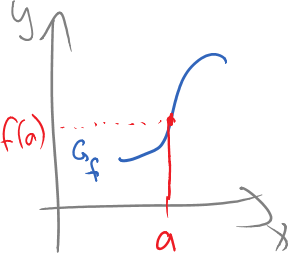
\includegraphics[width=\linewidth]{Bilder/137}
			stetig in $a$
		\end{minipage}
		\quad
		\begin{minipage}{0.3\linewidth}
			\centering
			\includegraphics[width=\linewidth]{Bilder/138}
			unstetig in $a$
		\end{minipage}
		\quad
		\begin{minipage}{0.3\linewidth}
			\centering
			\includegraphics[width=\linewidth]{Bilder/139}\\
			unstetig in $a$
		\end{minipage}
		\caption{}
	\end{figure}
	
	\item Alle ganzrationalen und gebrochenrationalen Funktionen sind stetig,\\
	alle Potenzfunktionen und Exponentialfunktionen sind stetig,\\
	alle trigonometrischen Funktionen sind stetig,\\
	alle Logarithmusfunktionen sind stetig.
	
	\item $\epsilon-\delta$-Kriterium der Stetigkeit\\
	$f$ ist stetig in $a\in\D\eq\forall\epsilon>0\exists\delta>0\forall x\in\D|x-a|<\delta\imp|f(x)-f(a)|<\epsilon$
\end{enumerate}

\Satz{{\bf Zwischenwertsatz}\\
	\\
	Sei $f:[a,b]\to\R$ stetig und es gelte $f(a)\cdot f(b)<0$.\\
	Dann existiert ein $x_0\in]a,b[$ mit $f(x_0)=0$.}

%bild 162
\imgw{Bilder/140}{}{}{5cm}

\clearpage
\chapter{Differentiation}
\section{Differenzierbarkeit}
\Problem Bestimmung der Steigung der Tangente an den Graphen von $f$ in Punkt $P(x_0;f(x_0))$

%bild 163
\imgw{Bilder/141}{}{}{8cm}

Sekantensteigung $m_{s,\Delta x} = \dfrac{\Delta y}{\Delta x} = \dfrac{f(x_0+\Delta x) - f(x_0)}{\Delta x}$

Für $\Delta x\to0$ geht die Sekante in die Tangente $t$ über (im Grenzfall)\\
Für die Steigung $m_t$ der Tangente $t$ gilt dann\\
$m_t=\lim\limits_{\Delta x\to0}m_{s,\Delta x} = \lim\limits_{\Delta x\to0}\dfrac{f(x_0+\Delta x) - f(x_0)}{\Delta x}$ (falls der Grenzwert sprich die Tangente existiert)

\Def
\begin{enumerate}[a)]
	\item $f:\D\to\R$ heißt \ul{differenzierbar in $x_0\in\D$}, wenn der Grenzwert\\
	$f'(x_0) := \lim\limits_{\Delta x\to0}\dfrac{f(x_0+\Delta x) - f(x_0)}{\Delta x}$\\
	existiert; $f'(x_0)$ heißt \ul{Differentialquotien in $x_0$} oder \ul{Ableitung von $f$ in $x_0$}; man schreibt auch\\
	$f'(x_0)=\df{f}{x}(x_0)$ (Leibniz-Schreibweise)\\
	(d$f$ und d$x$ heißen \ul{Differentiale})
	
	\item $f:\D\to\R$ heißt \ul{differenzierbar} (in $\D$), wenn $f$ differenzierbar in \ul{jedem} $x_0\in\D$ ist.
	
	\Bem $f:\D\to\R$ ist genau dann in $x_0\in\D$ differenzierbar, wenn die einseitigen Grenzwerte $\lim\limits_{\Delta x\to0^\pm}\dfrac{f(x_0+\Delta x) - f(x_0)}{\Delta x}$ existieren und übereinstimmen.
\end{enumerate}

\Satz{Ist $f:\D\to\R$ in $x_0\in\D$ differenzierbar, so ist $f$ in $x_0$ stetig\\
	{\flqq Differenzhierbarkeit\frqq}$\imp${\flqq Stetigkeit\frqq}.}

\Satz{Ist $f:]a;b[\to\R$ differenzierbar und gilt $f'(x)\begin{array}{c}>\\<\end{array}0$ in $]a;b[$, so ist $f$ streng monoton $\left\{\begin{array}{c}\text{steigend}\\\text{fallend}\end{array}\right\}$ auf $]a;b[$.}

%bild 164
\begin{figure}[h!]
	\centering
	\begin{minipage}{0.4\linewidth}
		\centering
		\includegraphics[width=3cm]{Bilder/142}
	\end{minipage}
	\qquad
	\begin{minipage}{0.4\linewidth}
		\centering
		\includegraphics[width=3cm]{Bilder/143}
	\end{minipage}
	\caption{}
\end{figure}

\Beachte Die Voraussetzung im obigen Satz, dass $\D=]a;b[$ ein Intervall ist, ist wesentlich, denn z.B. gilt für $f:\R\setminus\{0\}\to\R,x\mapsto\frac{1}{x}$ folgendes:\\
$f'(x)=-\frac{1}{x^2}<0$, jedoch ist $f$ \ul{nicht} streng monoton fallend.

Auf dem Jeweiligen Intervall $]-\infty;0[$ bzw. $]0;\infty[$ ist $f$ streng monoton fallend, jedoch nicht auf $\R\setminus\{0\}$.

%bild 165
\begin{figure}[h!]
	\centering
	\includegraphics[width=8cm]{Bilder/144}\\
	\begin{minipage}{4cm}
		\centering
		streng monoton\\
		fallend auf $]-\infty;0[$
	\end{minipage}
	\qquad
	\begin{minipage}{4cm}
		\centering
		streng monoton\\
		fallend auf $]0;\infty[$
	\end{minipage}
	\caption{}
\end{figure}

\Satz{{\bf Regel von L'Hospital}\\
	\\
	Führt die Betrachtung von $\lim\limits_{x\to x_0}\dfrac{f(x)}{g(x)}$ auf einen unbestimmten Ausdruck der Form {\flqq$\frac{0}{0}$\frqq} bzw. {\flqq$\frac{\infty}{\infty}$\frqq}, so gilt \redbox{$\lim\limits_{x\to x_0}\dfrac{f(x)}{g(x)} = \lim\limits_{x\to x_0}\dfrac{f'(x)}{g'(x)}$}\\
	Die Regel ist wiederholt anwendbar.}

Anwendung der L'Hospitalschen Regel auf weitere unbestimmte Ausdrücke durch vorherige Transformation.

\begin{tabular}{c|c|c}
	$\varphi(x)$ & \parbox{5cm}{$\lim\limits_{x\to x_0}\varphi(x)$ führt zu unbestimmten Ausdruck} & Transformation \\
	\hline
	$f(x)\cdot g(x)$ & {\flqq$0\cdot\infty$\frqq}, {\flqq$0\cdot-\infty$\frqq}& $\lim\limits_{x\to x_0}\dfrac{f(x)}{\frac{1}{g(x)}} = \lim\limits_{x\to x_0}\dfrac{g(x)}{\frac{1}{f(x)}}$\\
	\hline
	$f(x) - g(x)$ & {\flqq$\infty - \infty$\frqq}& $\lim\limits_{x\to x_0}\dfrac{\frac{1}{g(x)}-\frac{1}{f(x)}}{\frac{1}{f(x)\cdot g(x)}}$\\
	\hline
	${f(x)}^{g(x)}$ & {\flqq$0^0$\frqq}, {\flqq$\infty^0$\frqq}, {\flqq$1^{\pm\infty}$\frqq}& $\lim\limits_{x\to x_0}e^{g(x)\ln(f(x))}$ ($f(x)>0$)\\
\end{tabular}

\Bsp
\begin{enumerate}
	\item Die Betragsfunktion $|\ldots|:\R\to\R,x\mapsto |x|$ ist in $x=0$ \ul{nicht} differenzierbar.
	
	$|x| = \left\{
	\begin{array}{ll}
		x,&\text{falls }x\ge 0\\
		-x,&\text{falls }x<0\\
	\end{array}
	\right.$
	
	%bild 166
	\imgw{Bilder/145}{}{}{8cm}
	
	$\lim\limits_{\Delta x\to0^-}\dfrac{f(x_0+\Delta x) - f(x_0)}{\Delta x} = \lim\limits_{\Delta x\to0^-}\dfrac{|\Delta x| - |0|}{\Delta x} = \lim\limits_{\Delta x\to0^-}\dfrac{-\Delta x}{\Delta x} = -1$
	
	$\lim\limits_{\Delta x\to0^+}\dfrac{f(x_0+\Delta x) - f(x_0)}{\Delta x} = \lim\limits_{\Delta x\to0^+}\dfrac{|\Delta x| - |0|}{\Delta x} = \lim\limits_{\Delta x\to0^+}\dfrac{\Delta x}{\Delta x} = +1$
	
	$\Rightarrow$ einseitige Grenzwerte existieren, stimmen jedoch \ul{nicht} überein.
	
	\item $f(x) = \left\{
	\begin{array}{ll}
	(x-1)^2,&\text{falls }x<0\\
	(x+1)^2,&\text{falls }x\ge0\\
	\end{array}
	\right.$
	
	\Beh $f$ ist in $x=0$ \ul{nicht} differenzierbar (HÜ)
\end{enumerate}

\section{Ableitung erster und höherer Ordnung}
\Def
\begin{enumerate}[a)]
	\item Ist $f:\D\to\R$ differenzierbar (in $\D$), so heißt die Funktion $f':\D\to\R, x\mapsto f'(x)$ die \ul{Ableitung} von $f$.
	\item Ist die Ableitung $f':\D\to\R$ differenzierbar (in $\D$), so heißt $f''(x) = (f'(x))'$ die \ul{zweite Ableitung} von $f$;\\
	analog definiert man die \ul{$k$-te Ableitung} durch\\
	$f^{(k)}(x)=(f^{(k-1)}(x))'$,\\
	falls $f^{(k)}$ existiert.
\end{enumerate}

\Bsp
\begin{enumerate}
	\item $f(x) = x^2, f'(x)=2x, f''(x)=2$
	\item $f(x) = \sin(x), f'(x) = \cos(x), f''(x) = -\sin(x)$
	\item $f(x) = e^x, f'(x) = e^x, f''(x) = e^x$
	\item $f(x) = \ln x, f'(x) = \frac{1}{x}, f''(x) = -\frac{1}{x^2}$
\end{enumerate}

\section{Ableitungsregeln}
\Satz{Es seien $u,v$ differenzierbare Funktionen, $\alpha\in\R$.
	\begin{enumerate}[a)]
		\item Summenregel \redbox{$(u\pm v)' = u'\pm v'$}
		\item Faktorregel \redbox{$(\alpha u)' = \alpha\cdot u'$} ($\alpha$ = multiplikative Konstante)
		\item Produktregel \redbox{$(u\cdot v)' = u'\cdot v + u\cdot v'$}
		\item Quotientenregel \redbox{$\left(\dfrac{u}{v}\right)' = \dfrac{u'\cdot v - u\cdot v'}{v^2}$}
		\item Kettenregel \redbox{$\left(u\circ v\right)' = \left(u'\circ v\right)\cdot v'$} \red{Nachdifferenzieren = Multiplikation mit $v'$}\\
		bzw. $u(v(x))' = u'(v(x))\cdot v'(x)$\\
		bzw. $\df{u}{x} = \df{u}{v}\cdot\df{v}{x}$
	\end{enumerate}}

\subsection{Ableitung elementarer Funktionen}

\begin{tabular}{c|c}
	$f(x)$ & $f'(x)$\\
	\hline
	$x^n$ & $nx^{n-1}$ ($n\in\R$)\\
	$\sin x$ & $\cos x$\\
	$\cos x$ & $-\sin x$\\
	$\tan x$ & $\dfrac{1}{\cos^2 x}$\\
	$\cot x$ & $-\dfrac{1}{\sin^2 x}$\\
	$e^x$ & $e^x$\\
	$a^x$ & $a^x\cdot\ln a$\\
	$\ln x$ & $\dfrac{1}{x}$\\
	$\log_ax$ & $\dfrac{1}{x\cdot\ln a}$\\
	$\sqrt{x}$ & $\dfrac{1}{2\sqrt{x}}$\\
\end{tabular}

\Bem Mehrfaches Nachdifferenzieren

$u(v(w(x)))' = u'(v(w(x)))\cdot v(w(x))' = u'(v(w(x)))\cdot v'(w(x))\cdot w'(x)$

bzw. $\df{u}{x} = \df{u}{v}\cdot\df{v}{w}\cdot\df{w}{x}$

\Bsp $[\sin(\sqrt{x^2+1})]' = \cos(\sqrt{x^2+1})\cdot\dfrac{1}{2\sqrt{x^2+1}}\cdot 2x$

\section{Ableitung der Umkehrfunktion}
\Satz{Es sei $f:\D\to E$ eine differenzierbare, bijektive Funktion. Dann ist auch die Umkehrfunktion $f^{-1}:E\to\D$ differenzierbar und es gilt\\
	\redbox{${f^{-1}}'(x)=\dfrac{1}{f'(f^{-1}(x))}$}
	}

\Bsp
\begin{enumerate}
	\item $e^x:\R\to\Rp$ ist bijektiv.\\
	Umkehrfunktion $\ln x:\Rp\to\R$.
	
	$(\ln x)' = \dfrac{1}{e^{\ln x}} = \dfrac{1}{x}$
	
	\item $\sin:[-\frac{\pi}{2};\frac{\pi}{2}]\to[-1;1]$ bijektiv\\
	%bild 167
	\imgw{Bilder/146}{}{}{6cm}
	Umkehrfunktion $\arcsin(=\sin^{-1}):[-1;1]\to[-\frac{\pi}{2};\frac{\pi}{2}]$
	%bild 168
	\imgw{Bilder/147}{}{}{4.5cm}
	
	$\arcsin(x)'=\dfrac{1}{\cos(\arcsin(x))}$
	
	trigonometrischer Pythagoras: $\cos^2x+\sin^2x=1\\
	\Leftrightarrow\cos^2x=1-\sin^2x\\
	\underbrace{\Leftrightarrow}_{\cos x\ge0}\cos x = \sqrt{1-\sin^2x}$
	
	$\cos(\arcsin(x)) > 0 \quad (-\frac{\pi}{2}\le\arcsin x\le\frac{\pi}{2})$
	
	$\Rightarrow arcsin(x)'=\dfrac{1}{\sqrt{1-\sin^2(\arcsin(x))}} = \dfrac{1}{\sqrt{1-x^2}}$
	
	\item Ableitung $\arccos(x)$ HÜ
\end{enumerate}

\clearpage
\section{Extremwerte und Krümmung}
\Def $f:[a;b]\to\R$ besitzt bei $x_0\in]a;b[$ ein (isoliertes) $\left\{\begin{array}{c}\text{lokales Maximum}\\\text{lokales Minimum}\end{array}\right\}$, wenn $\left\{\begin{array}{c}f(x)<f(x_0)\\f(x)>f(x_0)\end{array}\right\}$ für alle $x\in U_\epsilon(x_0)\setminus\{x_0\}$ gilt (für ein $\epsilon>0$).\\
$U_\epsilon(x_0)=]x_0-\epsilon,x_0+\epsilon[$ {\flqq$\epsilon$-Umgebung von $x$\frqq}
%bild 170
\imgw{Bilder/148}{}{}{5cm}

Der Punkt $P(x_0;f(x_0))$ heißt dann $\left\{\begin{array}{c}\ul{\text{Hochpunkt (HP)}}\\\ul{\text{Tiefpunkt (TP)}}\end{array}\right\}$. Ein lokales Maximum/Minimum heißt auch \ul{lokales Extremum}.
%bild 171
\begin{figure}[h!]
	\centering
	\begin{minipage}{0.4\linewidth}
		\centering\includegraphics[width=\linewidth]{Bilder/149}
		\caption{lokales Maximum}
	\end{minipage}
	\qquad
	\begin{minipage}{0.4\linewidth}
		\centering\includegraphics[width=\linewidth]{Bilder/150}
		\caption{lokales Minimum}
	\end{minipage}
\end{figure}

$f$ hat bei $x_0\in[a;b]$ ein $\left\{\begin{array}{c}\text{globales Maximum}\\\text{globales Minimum}\end{array}\right\}$, wenn $\left\{\begin{array}{c}f(x)\le f(x_0)\\f(x)\ge f(x_0)\end{array}\right\}$ für \ul{alle} $x\in[a;b]$ gilt.

$f(x_0)$ heißt dann globales Maximum bzw. Minimum (von $f$).

\Bem hat $f$ bei $x_1,\ldots,x_n$ alle lokalen Extrema, so gilt:\\
globales Maximum/Minimum = Max/Min$\{f(a),f(x_1),\ldots,f(x_n),f(b)\}$ \red{Ränder des Intervalls berücksichtigen!}

\Def Hat $f:[a;b]\to\R$ bei $x=a$ oder $x=b$ (Ränder des Intervalls) ein globales Maximum/Minimum, so nennt man $f(x_0)$ ein \ul{Randmaximum}/\ul{Randminimum}.

%bild 172
\begin{figure}[h!]
	\centering
	\begin{minipage}{0.4\linewidth}
		\centering\includegraphics[width=\linewidth]{Bilder/151}
		\caption{}
	\end{minipage}
	\qquad
	\begin{minipage}{0.4\linewidth}
		\centering\includegraphics[width=\linewidth]{Bilder/152}
		\caption{}
	\end{minipage}
\end{figure}

\Satz{$f$ sei differenzierbar; $x_0\in]a;b[$\\
	$f$ hat bei $x_0$ ein lokales $\left\{\begin{array}{c}\text{Maximum}\\\text{Minimum}\end{array}\right\}$\\
	$\Leftrightarrow f'$ wechselt bei $x_0$ das Vorzeichen $\left\{\begin{array}{c}\text{von $+$ nach $-$}\\\text{von $-$ nach $+$}\end{array}\right\}$.}

\Satz{{\bf notwendiges Kriterium für Extremum}\\
	\\
	$f$ sei stetig differenzierbar, d.h. differenzierbar und $f'$ sei stetig.\\
	Besitzt $f$ bei $x_0\in]a;b[$ ein lokales Extremum, so gilt \redbox{$f'(x_0)=0$}}

\Satz{{\bf hinreichendes Kriterium für Extremum}\\
	\\
	$f$ sei zweimal stetig differenzierbar, d.h. $f''$ existiert und ist stetig.\\
	Gilt dann $f'(x_0)=0$ und $\left\{\begin{array}{c}f''(x_0)>0\\f''(x_0)<0\end{array}\right\}$ für ein $x_0\in]a;b[$, so hat $f$ bei $x_0$ ein (isoliertes) $\left\{\begin{array}{c}\text{lokales Minimum}\\\text{lokales Maximum}\end{array}\right\}$.}

\Bsp
\begin{enumerate}
	\item $f(x) = -2(x-3)^2+4$\\
	$f'(x) = -4(x-3) = -4x+12$\\
	$f''(x) = -4<0$\\
	$f'(x) = 0 \Leftrightarrow -4(x-3) = 0 \Leftrightarrow x=3$\\
	$\Rightarrow f$ hat bei $x=3$ ein lokales Maximum
	
	\item $f(x) = x^4$\\
	$f'(x) = 4x^3$\\
	$f''(x) = 12x^2$\\
	$f'(x) = 0 \Leftrightarrow 4x^3 = 0 \Leftrightarrow x = 0$\\
	Jedoch ist $f''(0)=0\Rightarrow$ Kriterium nicht anwendbar.\\
	$f'(x) = 4x^3$ hat aber bei $x=0$ einen Vorzeichenwechsel von $-$ nach $+$ $\Rightarrow f$ hat bei $x=0$ ein lokales Minimum.
	
	\item $f(x) = |x|$\\
	$f'(x) = \left\{\begin{array}{ll}
	+1,&\text{für }x>0\\
	-1,&\text{für }x<0\\
	\end{array}\right.$\\
	$f'(0)$ existiert nicht.\\
	$f'(x) = \sgn(x)\quad(x\ne0)$\\
	$f'(x)$ hat bei $x=0$ einen Vorzeichenwechsel von $-$ nach $+$ $\Rightarrow f$ hat bei $x=0$ ein lokales Minimum.
\end{enumerate}

\Def $f$ heißt in einer Umgebung $U_\epsilon(x_0)$ von $x_0$ (oder bei $x_0$ \gray{(mit kleiner Umgebung)}) $\left\{\begin{array}{c}\text{linksgekrümmt}\\\text{rechtsgekrümmt}\end{array}\right\}$, wenn die Ableitung $f'$ auf $U_\epsilon(x_0)$ $\left\{\begin{array}{c}\text{streng monoton steigt}\\\text{streng monoton fällt}\end{array}\right\}$.

%bild 173
\begin{figure}[h!]
	\centering
	\begin{minipage}{0.4\linewidth}
		\centering\includegraphics[width=\linewidth]{Bilder/153}
		\caption{linksgekrümmt}
	\end{minipage}
	\qquad
	\begin{minipage}{0.4\linewidth}
		\centering\includegraphics[width=\linewidth]{Bilder/154}
		\caption{rechtsgekrümmt}
	\end{minipage}
\end{figure}

\Satz{$f$ sei zweimal stetig differenzierbar. Dann gilt:\\
	\\
	$f$ ist bei $x_0$ $\left\{\begin{array}{c}\text{linksgekrümmt}\\\text{rechtsgekrümmt}\end{array}\right\}$ genau dann, wenn $\left\{\begin{array}{c}f''(x_0)>0\\f''(x_0)<0\end{array}\right\}$ gilt.}

\Def Der Zahlenwert \redbox{$\kappa = \dfrac{y''(x_0)}{(1+y'(x_0)^2)^{\frac{3}{2}}}$} heißt \ul{Krümmung} der Kurve $y=f(x)$ im Punkt $P(x_0;f(x_0))$\\
Mit \redbox{$\rho=\dfrac{1}{|\kappa|}$} bezeichne man den \ul{Krümmungsradius}.

\Bem $\rho$ ist der Radius des Krümmungskreises (Schmiegkreis) an die Kurve $y=f(x)$ im Punkt $P(x_0;f(x_0))$.
%bild 174
\imgw{Bilder/155}{$\rho$ = Krümmungsradius}{}{8cm}

\Bsp Behauptung: Ein Kreis mit Radius $R$ hat konstante Krümmung $|\kappa|=\dfrac{1}{R}$.
%bild 175
\img{Bilder/156}{}{}

$x^2+y^2=R^2$

Kreisgleichung nach $y$ umstellen

\begin{align*}
x^2+y^2 &= R^2\\
\Leftrightarrow y^2 &= R^2-x^2\mid\pm\sqrt{\ }\\
\Leftrightarrow y &= \pm\sqrt{R^2-x^2}\\
\end{align*}

Berechne Krümmung $\kappa$ für oberen Halbkreis:

\begin{align*}
y &= \sqrt{R^2-x^2}\\
y' &= \dfrac{1}{2\sqrt{R^2-x^2}}\cdot(-2x) = \dfrac{-x}{\sqrt{R^2-x^2}}\\
y'' &= \dfrac{-\sqrt{R^2-x^2}+x\cdot\dfrac{-x}{\sqrt{R^2-x^2}}}{R^2-x^2} =  HÜ\\
\end{align*}

\Def $W(x_0;f(x_0))$ heißt Wendepunkt von $f:\D\to\R,x_0\in\D$, wenn $f$ bei $x_0$ das Krümmungsverhalten wechselt.

\begin{figure}[h!]
	\begin{minipage}{0.49\linewidth}
		\centering \includegraphics[width=0.7\linewidth]{Bilder/157}
	\end{minipage}
	\begin{minipage}{0.49\linewidth}
		\centering \includegraphics[width=0.7\linewidth]{Bilder/158}
	\end{minipage}
	\caption{}
\end{figure}

Gleichwertig mit dem Wechsel des Krümmungsverhaltens ist der Wechsel des Vorzeichens der zweiten Ableitung $f''$ bei $x=x_0$.

\Satz{{\bf hinreichendes Kriterium für WP}\\
	\\
	$f$ sei 3-mal differenzierbar und $f'''$ sei in $x_0$ stetig.\\
	$x_0\in]a;b[$.\\
	Gilt dann $f''(x)=0$ und $f'''(x)\ne0$, so hat $f$ bei $x_0$ einen Wendepunkt.}

\Bem Ist z.B. $f'''(x_0)=0$, so kann obiges Kriterium nicht verwendet werden $\rightarrow$ Vorzeichenwechsel von $f'''$ bei $x=x_0$ nachweisen.

\chapter{Elementare Funktionen und Kurven}
\section{Potenzfunktionen}
\Def Funktionen der Form \redbox{$f(x)=a\cdot x^r$} ($a,r\in\R$) heißen \ul{Potenzfunktionen}.

\begin{enumerate}[A)]
	\begin{figure}[h!]
		\item \ul{Ganzzahlige Exponenten} $r=n\in\Z$\\
		
		\grayframe{$n>0$} ($\D=\R$)
		
		\begin{minipage}{0.49\linewidth}
			\centering \includegraphics[width=0.9\linewidth]{Bilder/159}
			\caption{$n$ gerade (Achsen-symmetrisch)}
		\end{minipage}
		\begin{minipage}{0.49\linewidth}
			\centering \includegraphics[width=0.7\linewidth]{Bilder/160}
			\caption{$n$ ungerade (Punkt-symmetrisch)}
		\end{minipage}
	\end{figure}
	
	\begin{figure}[h!]
		\grayframe{$n<0$} ($\D=\R\setminus\{0\}$)
		
		\begin{minipage}{0.49\linewidth}
			\centering \includegraphics[width=0.9\linewidth]{Bilder/161}
			\caption{$n$ gerade (Achsen-symmetrisch)}
		\end{minipage}
		\begin{minipage}{0.49\linewidth}
			\centering \includegraphics[width=0.7\linewidth]{Bilder/162}
			\caption{$n$ ungerade (Punkt-symmetrisch)}
		\end{minipage}
	\end{figure}
	
	\begin{figure}[h!]
		\item \ul{Rationale Exponenten} $r\frac{p}{q}, p\in\Z,q\in\N,r\not\in\Z$
		
		\begin{minipage}{0.49\linewidth}
			\grayframe{$n>0$} ($\D=\Rop$) $\qquad x^\frac{p}{q}=\sqrt[q]{x^p}$
			
			\centering \includegraphics[width=0.9\linewidth]{Bilder/163}
			\caption{}
		\end{minipage}
		\begin{minipage}{0.49\linewidth}
			\grayframe{$n<0$} ($\D=\Rp$)
			
			\centering \includegraphics[width=0.9\linewidth]{Bilder/164}
			\caption{}
		\end{minipage}
	\end{figure}
	
	\begin{figure}[h!]
		\item \ul{Irrationaler Exponent} z.B. $r=\sqrt{2} = 1{,}4142\ldots$
			
		\begin{minipage}{0.49\linewidth}
			\centering \includegraphics[width=0.9\linewidth]{Bilder/165}
			\caption{}
		\end{minipage}
	\end{figure}
\end{enumerate}

\clearpage
\begin{minipage}{\linewidth}
	Umkehrfunktion zu $f(x)=x^r$ ist $f^{-1}(x)=x^{\frac{1}{r}}$\\
	$G_{f^{-1}}$ durch Spiegelung von $G_{f}$ an der Winkelhalbierenden $y=x$.
	
	\paragraph{Ableitung:} $(x^r)' = rx^{r-1}\qquad(r\in\R)$
	
	\paragraph{Grenzwerte:} für $x\to\pm\infty$
	\begin{align*}
	\lim\limits_{x\to\pm\infty}x^r&=\left\{\begin{array}{ll}+\infty&,\text{falls }r\text{ gerade}\\\pm\infty&,\text{falls }r\text{ ungerade}\end{array}\right.\qquad r\in\Z, r>0\\
	\lim\limits_{x\to+\infty}x^r&=+\infty\text{ für }r\not\in\Z,r>0\\
	\lim\limits_{x\to\pm\infty}x^r&=0\text{ für }r\in\Z, r<0\\
	\lim\limits_{x\to+\infty}x^r&=0\text{ für }r\not\in\Z,r<0\\
	\end{align*}
\end{minipage}

\clearpage
\section{Ganzrationale Funktionen}
\Def Funktionen der Form\\
$f(x)=a_nx^n+a_{n-1}x^{n-1}+\ldots+a_1x+a_0 \\(a_0,\ldots,a_n\in\R, a_n\ne0)$ heißen \ul{ganzrationale Funktionen}, $n$ ist der \ul{Grad} von $f$; $n=\grad(f)$.

\begin{itemize}
	\item $n=1$: $f(x)=a_1x+a_0$\quad \ul{lineare Funktionen}
	\item $n=2$: $f(x)=a_2x^2+a_1x+a_0$\quad \ul{quadratische Funktionen}
	\item $n=3$: $f(x)=a_3x^3+a_2x^2+a_1x+a_0$\quad \ul{kubische Funktionen}
\end{itemize}

\paragraph{Nullstellen mit Vielfachheiten}
\Satz{Ist $x_0$ eine Nullstelle einer ganzrationalen Funktion $f(x)$ vom Grad $n$ so kann $f(x)$ geschrieben werden als\\
	\redbox{$f(x)=(x-x_0)^r\cdot g(x)$}\\
	mit $g(x_0)\ne0$; $g(x)$ ist eine ganzrationale Funktion vom Grad $n-r$\\
	$r$ heißt \ul{Vielfachheit} der Nullstelle $x_0$ von $f$}

\Bem Die Darstellung erhält man durch (sukzessive) Polynomdivision.
\Satz{{\bf Hauptsatz der (reellen) Algebra}\\
	\\
	Jede ganzrationale Funktion $f(x)$ vom Grad $n\ge1$ besitzt eine Darstellung der Form\\
	\redbox{$f(x)=a\cdot(x-x_1)^{e_1}\cdot(x-x_2)^{e_2}\cdot\ldots\cdot(x-x_r)^{e_r}\cdot q_1\cdot\ldots\cdot q_s$}\\
	vorbei $x_1,\ldots,x_r$ die Nullstellen von $f(x)$ mit Vielfachheiten $e_1,\ldots,e_r$, $a\in\R$ und $q_1,\ldots,q_s$ (Unzerlegbare, d.h. Diskriminante $D<0$) quadratische ganzrationale Funktionen sind. Obige Darstellung heißt \ul{vollständige Faktorisierung} von $f(x)$. Die Faktoren $(x-x_i)$ heißen \ul{Linearfaktoren} $(i=1,\ldots,r)$.}

\paragraph{Folgerung:}
Eine ganzrationale Funktion $f(x)$ vom Grad $n\ge1$ besitzt (mit Vielfachheiten gezählt) höchstens $n$ Nullstellen.

\Bsp $f(x) = 2x^5-4x^4+2x^3+2x^2-4x+2$\\
Finde Nulstellen von $f(x)$ durch {\flqq Probieren\frqq} Teste alle Teiler des {\flqq konstanten Glieds\frqq}, hier $2$:\\
$\pm1;\pm2\Rightarrow f(1) = 0$\\
$\Rightarrow$ Polynomdivision $f(x):(x-1) = 2x^4-2x^3+0x^2+2x-2$

$f(x):(x-1) = 2x^4-2x^3+0x^2+2x-2\quad\mid\cdot(x-1)$\\
$f(x) = \red{\underbrace{\black{(x-1)}}_\text{Linearfaktor}}\cdot\red{\underbrace{\black{(2x^4-2x^3+0x^2+2x-2)}}_{f_1(x)}}$\\
$f_1(1) = 0\qquad\Rightarrow$ Polynomdivision $f_1(x):(x-1) = 2x^3+0x^2+0x+2$

$f_1(x) = (x-1)\cdot(2x^3+2) = 2\cdot \red{\underbrace{\black{(x-1)}}_\text{Linearfaktor}}\cdot\red{\underbrace{\black{(x^3+1)}}_{f_2(x)}}$\\
$f(x) = 2\cdot(x-1)^2\cdot\red{\underbrace{\black{(x^3+1)}}_{f_2(x)}}$

Wegen $f_2(1)\ne0$ kann kein weiterer Linearfaktor $(x-1)$ durch Polynomdivision abgespalten werden.

Da $f_2(-1)=0\qquad\Rightarrow$ Polynomdivision $f_2(x):(x+1) = x^2-x+1$\\
$f_2(x) = \red{\underbrace{\black{(x+1)}}_\text{Linearfaktor}}\cdot\red{\underbrace{\black{(x^2-x+1)}}_{f_3(x)}}$

Für $f(x)$ folgt: $f(x) = 2\cdot(x-1)^2(x+1)(x^2-x+1)$\qquad(*)

Die quadratische Funktion $x^2-x+1$ ist (über $\R$) unzerlegbar, da für die Diskriminante $D=1-4<0$ gilt.

$\Rightarrow$ (*) ist vollständige Faktorisierung von $f(x)$\\
$f(x)$ hat die Nullstellen:\\
$x_1=1$\quad(2-fach)\\
$x_2=-1$\quad(1-fach)

Der quadratische Faktor $x^2-x+1$ ist stets positiv, d.h. $x^2-x+1>0$ für alle $x\in\R$

\clearpage
\ul{VZT für $f(x)$:}

\begin{tabular}{c|c|c|c|c|c}
	& $-\infty<x<-1$ & $x=-1$ & $-1<x<1$ & $x=1$ & $1<x<\infty$\\
	\hline
	$2$ & $+$ & $+$ & $+$ & $+$ & $+$\\
	$x+1$ & $-$ & $0$ & $+$ & $+$ & $+$\\
	$(x-1)^2$ & $+$ & $+$ & $+$ & $0$ & $+$\\
	$x^2-x+1$ & $+$ & $+$ & $+$ & $+$ & $+$\\
	\hline
	$f(x)$ & $-$ & $0$ & $+$ & $0$ & $+$\\
\end{tabular}

\clearpage
\paragraph{Skizze:} $f(0)=2$
\imgw{Bilder/166}{}{}{5cm}

\clearpage
Verlauf von $G_f$ in der Nähe von einer Nullstelle $x_0$ mit Vielfachheit $r$.
\begin{figure}[h!]
	\centering
	\begin{longtable}{ccc}
		\includegraphics[width=3cm]{Bilder/167} &
		\includegraphics[width=3cm]{Bilder/168} &
		\includegraphics[width=3cm]{Bilder/169} \\
		
		\includegraphics[width=3cm]{Bilder/170} &
		\includegraphics[width=3cm]{Bilder/171} &
		\includegraphics[width=3cm]{Bilder/172} \\
		
		$r=1$ & $r>1$ gerade & $r>1$ ungerade \\
	\end{longtable}
	\caption{}
\end{figure}

\ul{Umkehrfunktion}: meist nur stückweise definiert (auf Intervallen, in denen $f$ streng monoton steigt/fällt).

\ul{Ableitung}: $f'(x)=na_nx^{n-1}+(n-1)a_{n-1}x^{n-2}+\ldots+a_22x+a_1$

\ul{Grenzwerte}:
\redframe{$\lim\limits_{x\to\pm\infty} a_nx^n+a_{n-1}x^{n-1}+\ldots+a_1x+a_0=\lim\limits_{x\to\pm\infty} a_nx^n$}

Der Term $a_nx^n$ heißt \ul{Leitterm} von $f(x)=a_nx^n+\ldots+a_0$. Das Verhalten von $f(x)$ im Unendlichen wird durch das Verhalten des Leitterms im Unendlichen bestimmt.

\Beweis $\lim\limits_{x\to\pm\infty} a_nx^n+\ldots+a_0=\lim\limits_{x\to\pm\infty}\left(a_nx^n\right)\left(\red{\underbrace{\black{1+\dfrac{a_{n-1}}{a_n}\dfrac{1}{x}+\dfrac{a_{n-2}}{a_n}\dfrac{1}{x^2}+\ldots+\dfrac{a_1}{a_n}\dfrac{1}{x^{n-1}}+\dfrac{a_0}{a_n}\dfrac{1}{x^n}}}_{\to1}}\right)=\lim\limits_{x\to\pm\infty} a_nx^n$

\clearpage
\section{gebrochen rationale Funktionen}
\Def Funktionen der Form\\
\redbox{$f(x)=\dfrac{Z(x)}{N(x)}$}\\
wobei $Z(x),N(x)$ ganzrationale Funktionen sind, heißen \ul{gebrochen-rationale Funktionen}.

Ist $\grad(Z(x))<\grad(N(x))$, so heißt $f(x)$ \ul{echt} gebrochen-rational, ansonsten \ul{unecht} gebrochen-rational.

\ul{Maximale Definitionsmenge}: $\D=\R\setminus\{x\mid N(x) = 0\}$

\ul{Nullstellen}: $x_0$ ist Nullstelle von $f(x)$\\
$\Leftrightarrow Z(x_0)=0$ und $x_0\in\D$\\
$\Leftrightarrow Z(x_0)=0$ und $N(x_0)\ne0$

\ul{Definitionslücken}: Definitionslücken = Nullstellen des Nenners $N(x)$
\begin{itemize}
	\item \redframe{Polstellen}
	\item \redframe{Hebbare Definitionslücken}
\end{itemize}

$x_0$ ist \ul{Polstelle} von $f(x)=\dfrac{Z(x)}{N(x)}$, wenn $|f(x)|$ (=Betrag von $f(x)$) in einer Umgebung $U_\epsilon(x_0)$ unbegrenzt wächst, d.h. falls\\
\redbox{$\lim\limits_{x\to x_0^+}f(x)=\pm\infty, \lim\limits_{x\to x_0^-}f(x)=\pm\infty$}\\
$x_0$ ist \ul{hebbare} Definitionslücke von $f(x)=\dfrac{Z(x)}{N(x)}$, wenn\\
\redbox{$\lim\limits_{x\to x_0}f(x) = c < \infty$} gilt.

\Satz{{\bf hinreichendes Kriterium für Polstelle}\\
	\\
	Gilt $Z(x_0)\ne0$ und $N(x_0)=0$, so hat $f(x)=\dfrac{Z(x)}{N(x)}$ bei $x = x_0$ einen Pol, d.h. $x_0$ ist eine Polstelle.}

\ul{Allgemeine Vorgehensweise zur Bestimmung der Polstellen}
(mit entsprechender Ordnung) von $f(x)=\dfrac{Z(x)}{N(x)}$
\begin{enumerate}
	\item Zerlege $Z(x)$ und $N(x)$ vollständig in lineare und (unzerlegbare) quadratische Faktoren (vollständige Faktorisierung)
	\item Kürze anschließend gleiche Faktoren von Zähler und Nenner $\Rightarrow$ neuer Zähler $Z^*(x)$, neuer Nenner $N^*(x)$\\
	$Z^*(x)$ und $N^*(x)$ haben keine gemeinsamen (reellen) Nullstellen und es gilt:\\
	$f(x)=\dfrac{Z(x)}{N(x)} = \dfrac{Z^*(x)}{N^*(x)}\qquad (\text{auf }\D)$\\
	Die Polstellen von $f(x)$ sind genau die Nullstellen von $N^*(x)$, die Vielfachheiten der Nullstelle von $N^*(x)$ sind die sogenannten \ul{Ordnungen} der Polstellen (oder Pole).
\end{enumerate}

\Bem Ist $x_0$ eine hebbare Definitionslücke, d.h. $N(x_0)=0$ und $x_0$ ist keine Polstelle, so besitzt der Graph von $f$ an der Stelle $L(x_0;y_0)$ ein {\flqq Loch\frqq}.
\imgw{Bilder/173}{}{}{6cm}

Dabei gilt:\\
$y_0=\lim\limits_{x\to x_0}f(x)=\lim\limits_{x\to x_0}\dfrac{Z(x)}{N(x)}=\lim\limits_{x\to x_0}\dfrac{Z^*(x)}{N^*(x)}=\dfrac{Z^*(x_0)}{N^*(x_0)}$\\
also:\\
\redbox{$y_0=\dfrac{Z^*(x_0)}{N^*(x_0)}$}\\
$N^*(x_0)\ne0$, da $x_0$ eine hebbare Definitionslücke ist.

\Bsp
\begin{enumerate}
	\item $f(x) = \dfrac{(x-1)^2(x+1)}{(x-2)^2(x+2)}=\dfrac{Z(x)}{N(x)}$
	
	keine gemeinsamen Faktoren: $Z(x) = Z^*(x), N(x) = N^*(x)$\\
	$\Rightarrow \dfrac{Z(x)}{N(x)} = \dfrac{Z^*(x)}{N^*(x)}$
	
	$\Rightarrow$ \ul{Nullstellen}:\\
	$x_1=1$\quad (2-fach) (kein VZW)\\
	$x_2=-1$\quad (1-fach) (VZW)
	
	$\Rightarrow$ \ul{Polstellen}:\\
	$x_{p1}=2$\quad (Ordnung 2) (kein VZW)\\
	$x_{p2}=-2$\quad (Ordnung 1) (VZW)
	
	alle Definitionslücken sind Polstellen $\Rightarrow$ keine hebbaren Definitionslücken
	%Bild Graph mit Asymptoten der Polstellen
	\imgw{Bilder/184}{}{}{7cm}
	
	\clearpage
	\item $f(x)=\dfrac{(x-1)(x+2)}{(x-1)^3}=\dfrac{Z(x)}{N(x)}$
	
	Definitionslücke: $x_1=1\Rightarrow$ maximale Definitionsmenge $\D=\R\setminus\{1\}$
	
	$\Rightarrow$ Bruchterm vollständig Kürzen:\\
	$f(x)=\dfrac{x+2}{(x-1)^2} = \dfrac{Z^*(x)}{N^*(x)}$
	
	$\Rightarrow$ \ul{Nullstellen}:\\
	$x_{n1} = -2$\quad(1-fach) (VZW)
	
	$\Rightarrow$ \ul{Polstellen}:\\
	$x_{p1} = 1$\quad(2. Ordnung) (kein VZW)
	
	%Bild Graph Asymptoten
	\imgw{Bilder/185}{}{}{7cm}
	
	\clearpage
	\item $f(x) = \dfrac{2(x-2)^2(x+5)}{(x-1)(x-2)(x+5)}$
	
	Definitionslücken: $x_1=-5,x_2=1,x_3=2$
	
	$\Rightarrow$ maximale Definitionsmenge $\D=\R\setminus\{-5;1;2\}$
	
	Bruchterm vollständig Kürzen:\\
	$f(x)=\dfrac{2(x-2)}{x-1}=\dfrac{Z^*(x)}{N^*(x)}$
	
	$\Rightarrow$ \ul{Nullstellen}:\\
	$Z^*(x)=0\Leftrightarrow x=2 \not\in\D\Rightarrow f\text{ hat \ul{keine} Nulstellen}$
	
	$\Rightarrow$ \ul{Polstellen}:\\
	$x_{p1} = 1$\quad(1. Ordnung) (VZW)
	
	\ul{Hebbare Definitionslücken}:\\
	$x_{h1} = -5;x_{h2} = 2$\quad($\Rightarrow$ 2 Löcher im Graphen)\\
	$y_{h1} = \lim\limits_{x\to x_{h1}}f(x) = \lim\limits_{x\to x_{h1}}\dfrac{Z(x)}{N(x)} = \lim\limits_{x\to x_{h1}}\dfrac{Z^*(x)}{N^*(x)} = \lim\limits_{x\to x_{h1}}\dfrac{Z^*(-5)}{N^*(-5)} = \dfrac{-14}{-6} = \dfrac{7}{3}$\\
	$y_{h2} = \lim\limits_{x\to x_{h2}}f(x) = \lim\limits_{x\to x_{h2}}\dfrac{Z(x)}{N(x)} = \lim\limits_{x\to x_{h2}}\dfrac{Z^*(x)}{N^*(x)} = \lim\limits_{x\to x_{h2}}\dfrac{Z^*(2)}{N^*(2)} = 0$\\
	
	%bild Graph mit Asymptoten Deflücken
	\imgw{Bilder/186}{}{}{7cm}
\end{enumerate}

\clearpage
\paragraph{Asymptoten:}
\begin{itemize}
	\item senkrechte Asymptoten:\\
	Ist $x_0$ eine Polstelle von $f(x) = \dfrac{Z(x)}{N(x)}$, so ist die senkrechte Gerade $x=x_0$ eine Asymptote von $f(x)$.
	\item Asymptoten im Unendlichen:\\
	Eine Funktion $p(x)$ heißt Asymptoten von $f(x)$ für $x\to\pm\infty$, wenn\\
	\redbox{$\lim\limits_{x\to+\infty}f(x)-p(x) = 0$ bzw. $\lim\limits_{x\to-\infty}f(x)-p(x) = 0$}.
	
	\Satz{\hfill}
	
	\begin{enumerate}
		\item\label{asymp1} Ist $f(x)=\dfrac{Z(x)}{N(x)}$ eine \ul{echt} gebrochen-rationale Funktion, so gilt $\lim\limits_{x\to\pm\infty}\dfrac{Z(x)}{N(x)}=0$, d.h. die Gerade $y=0$ ($\entspricht$ $x$-Achse) ist Asymptote für $f(x)=\dfrac{Z(x)}{N(x)}$ für $x\to+\infty$ und für $x\to-\infty$.
		
		\item Ist $f(x)=\dfrac{Z(x)}{N(x)}$ eine \ul{unecht} gebrochen-rationale Funktion, d.h. $\grad(Z(x))\ge\grad(N(x))$, so erhält man aus der Polynomdivision (mit Rest) $Z(x):N(x)$ eine ganz-rationale Funktion $p(x)$ und eine \ul{echt} gebrochen-rationale Funktion $\dfrac{R(x)}{N(x)}$ mit $\dfrac{Z(x)}{N(x)}=p(x)+\dfrac{R(x)}{N(x)}$ \qquad($R(x)$ = Rest der Polynomdivision)
		
		Dann ist $p(x)$ Asymptote für $f(x)=\dfrac{Z(x)}{N(x)}$ für $x\to+\infty$ und für $x\to-\infty$, denn\\
		$\lim\limits_{x\to\pm\infty}f(x)-p(x)=\lim\limits_{x\to\pm\infty}\dfrac{Z(x)}{N(x)}-p(x)=\lim\limits_{x\to\pm\infty}\dfrac{R(x)}{N(x)}=0$ (siehe \ref*{asymp1}.)
		
		Die Nullstellen von $\dfrac{R(x)}{N(x)}$ sind genau die Schnittstellen (= x-Koordinaten der Schnittpunkte) von $f(x)$ mit der Asymptote $p(x)$.
	\end{enumerate}
	
	\Bsp $f(x)=\dfrac{\frac{1}{2}x^3-\frac{3}{2}x+1}{x^2+3x+2}$ (unecht gebrochen-rationale Funktion)
	
	$Z(x)=\frac{1}{2}x^3-\frac{3}{2}x+1 = \frac{1}{2}(x^3-3x+1)$\\
	$Z(1) = 0$
	
	$\Rightarrow(x^3-3x+2):(x-1)=x^2+x-2$
	
	$\Rightarrow Z(x)=\frac{1}{2}(x^2+x-2)(x-1)$
	
	$x^2+x-2$ weiter zerlegen: Diskriminante $D=1-4(-2)=9>0$\\
	$x_{1/2}=\dfrac{-1\pm3}{2}\quad x_1=-2, x_2=1$
	
	$\Rightarrow Z(x)=\frac{1}{2}(x+2)(x-1)^2$
	
	Analog für Nennerpolynom: $N(x)=x^2+3x+2=(x+1)(x+2)$
	
	Somit folgt:\\
	$f(x)=\dfrac{Z(x)}{N(x)}=\dfrac{\frac{1}{2}(x-1)^2(x+2)}{(x+1)(x+2)} =\dfrac{\frac{1}{2}(x-1)^2}{x+1}= \dfrac{(x-1)^2}{2(x+1)}=\dfrac{Z^*(x)}{N^*(x)}$
	
	\ul{Definitionslücken}: $x_1=-1, x_2=-2$
	
	\ul{maximale Definitionsmenge}: $\D=\R\setminus\{-2;-1\}$
	
	\ul{Nullstellen}: $x_n=1\in\D$\quad(2-fach)
	
	\ul{Polstellen}: $x_p=-1$\quad(1. Ordnung) (VZW)
	
	\ul{hebbare Definitionslücke}: $x_h=-2$\\
	$y_h=\lim\limits_{x\to x_h}f(x)=\dfrac{Z^*(-2)}{N*(-2)}=-4{,}5$
	
	\ul{Asymptoten}:\\
	senkrechte Asymptote: $x=-1$\\
	Asymptote im Unendlichen: Polynomdivision $Z(x):N(x)$ bzw. $Z^*(x):N^*(x)=(x-1)^2:2(x+1)$
	
	$(x^2-2x+1):(2x+2)=\frac{1}{2}x-\frac{3}{2}$ $R(x)=4$
	
	$\Rightarrow f(x)=\frac{1}{2}x-\frac{3}{2}+\dfrac{4}{2x+2}=\frac{1}{2}x-\frac{3}{2}+\dfrac{2}{x+1}$
	
	$\Rightarrow$ Asymptote für $x\to\pm\infty$\\
	$p(x)=\frac{1}{2}x-\frac{3}{2}$
	
	%Bild
	\imgw{Bilder/187}{}{}{7cm}
\end{itemize}

\clearpage
\section{Exponential- und Logarithmusfunktionen}
\Def Funktionen der Form $f(x)=a^x$ $(a>0,a\ne0)$ (oder allgemein $f(x)=c\cdot a^x,c\in\R,c\ne0$) heißen \ul{Exponentialfunktionen} ($\D=\R$)

\ul{$a>1$}:
\begin{figure}[h!]
	%Bild 1
	\begin{minipage}{0.48\linewidth}
		\centering\includegraphics[height=4.5cm]{Bilder/188}
		\caption{}
	\end{minipage}
	\begin{minipage}{0.30\linewidth}
		streng monoton steigend
		
		$\lim\limits_{x\to+\infty}a^x=\infty$
		
		$\lim\limits_{x\to-\infty}a^x=0$
	\end{minipage}
\end{figure}

\ul{$0<a<1$}:
\begin{figure}[h!]
	%Bild 2
	\begin{minipage}{0.48\linewidth}
		\centering\includegraphics[height=4.5cm]{Bilder/189}
		\caption{}
	\end{minipage}
	\begin{minipage}{0.30\linewidth}
		streng monoton fallend
		
		$\lim\limits_{x\to+\infty}a^x=0$
		
		$\lim\limits_{x\to-\infty}a^x=\infty$
	\end{minipage}
\end{figure}

\clearpage
Für $a=e=2{,}71\ldots$ Eulersche Zahl heißt $e^x=\exp(x)$ \ul{natürliche Exponentialfunktion}:
%Bild 3
\imgw{Bilder/190}{}{}{7cm}

Ableitung: $(a^x)'=a^x\cdot\ln(a)$ (insbesondere $(e^x)'=e^x$)

\Def Funktionen der Form $f(x)=\log_a(x)$ $(a>0,a\ne0)$ heißen Logarithmusfunktionen ($\D=\Rp$)

\ul{$a>0$}:
\begin{figure}[h!]
	%Bild 4
	\begin{minipage}{0.48\linewidth}
		\centering\includegraphics[height=4.5cm]{Bilder/191}
		\caption{}
	\end{minipage}
	\begin{minipage}{0.30\linewidth}
		streng monoton steigend
		
		$\lim\limits_{x\to\infty}\log_a(x)=\infty$
		
		$\lim\limits_{x\to0^+}\log_a(x)=-\infty$
	\end{minipage}
\end{figure}

\ul{$0<a<0$}:
\begin{figure}[h!]
	%Bild 5
	\begin{minipage}{0.48\linewidth}
		\centering\includegraphics[height=4.5cm]{Bilder/192}
		\caption{}
	\end{minipage}
	\begin{minipage}{0.30\linewidth}
		streng monoton fallend
		
		$\lim\limits_{x\to\infty}\log_a(x)=-\infty$
		
		$\lim\limits_{x\to0^+}\log_a(x)=\infty$
	\end{minipage}
\end{figure}

\Satz{($a>0,a\ne0$)\\
	\\
	\redbox{$y=a^x\Leftrightarrow x=\log_a(y)$}\\
	d.h. $\log_a(x)= \inv{f}(x)$ ist die Umkehrfunktion von $a^x=f(x)$}

%Bild 6
\imgw{Bilder/193}{$a>1$}{}{5cm}

Ableitung: $(\log_ax)'=\dfrac{1}{x\cdot\ln a}$ (insbesondere $(\ln x)'=\dfrac{1}{x}$)

$\log_b(x) = \dfrac{\log_a(x)}{\log_a(b)}$

\clearpage
\section{Trigonometrischen Funktionen}
\Def Als \ul{trigonometrischen Funktionen} bezeichnet man die Funktionen $\sin x, \cos x, \tan x$ und $\cot x$.
\begin{itemize}
	\item $\sin x:\R\to[-1;1],\cos x:\R\to[-1;1]$
	%Bild sin cos
	\imgw{Bilder/194}{}{}{11cm}
	
	\ul{Nullstellen}:\\
	$\sin x=0\quad x_k=k\pi\quad(k\in\Z)$\\
	$\cos x=0\quad x_k=\frac{\pi}{2}k\pi\quad(k\in\Z)$
	
	\ul{Periode}: jeweils $2\pi$
	
	\ul{Ableitung}:\\
	$(\sin x)'= \cos x$\\
	$(\cos x)'= -\sin x$
	
	\ul{Symmetrie}:\\
	$\sin(-x)=-\sin(x)$ (ungerade Funktion, punktsymmetrisch)\\
	$\cos(-x)=\cos(x)$ (gerade Funktion, achsensymmetrisch)\\
	
	\clearpage
	\item allgemeine Sinusfunktion/Cosinusfunktion:
	
	$y=a\sin(bx+c), y=a\cos(bx+c)$
	
	%Bild
	\begin{figure}[h!]
		\graybox{$a>0$}\\
		\begin{minipage}{0.48\linewidth}
			\centering\includegraphics[width=7cm]{Bilder/195}
			\caption{}
		\end{minipage}
		\begin{minipage}{0.48\linewidth}
			$bx_0+c=0$\\
			$\Leftrightarrow$\redbox{$x_0=-\dfrac{c}{b}$}
			
			$b(x_0+p)+c=2\pi$\\
			$\Leftrightarrow p=\dfrac{2\pi-c}{b}-x_0$\\
			$\Leftrightarrow p=\dfrac{2\pi}{b}-\dfrac{c}{b}+\dfrac{c}{b}$\\
			$\Leftrightarrow$\redbox{$p=\dfrac{2\pi}{b}$}
		\end{minipage}
		(bei $a<0$ Spiegelung an $x$-Achse)
	\end{figure}
	
	%Bild
	\begin{figure}[h!]
		\graybox{$a>0$}\\
		\begin{minipage}{0.48\linewidth}
			\centering\includegraphics[width=7cm]{Bilder/196}
			\caption{}
		\end{minipage}
		\begin{minipage}{0.48\linewidth}
			analog gilt:\\
			\redbox{$x_0=-\dfrac{c}{b}$}
			
			\redbox{$p=\dfrac{2\pi}{b}$}
		\end{minipage}
		(bei $a<0$ Spiegelung an $x$-Achse)
	\end{figure}
	
	\parbox{\linewidth}{
	Sinusschwingung: $y=a\sin(\omega t+\alpha_0)$\\
	Cosinusschwingung: $y=a\sin(\omega t+\alpha_0)$\\
	$t_0=-\frac{\alpha_0}{\omega}$ {\flqq Startwert\frqq}\\
	$T=\frac{2\pi}{\omega}$ Periode}
	
	\clearpage
	\item $\tan x:\D\to\R$\qquad $\D=\R\setminus\{\frac{\pi}{2}+k\pi\mid k\in\Z\}$
	%Bild tan mit Asymptoten
	\imgw{Bilder/197}{}{}{11cm}
	
	\ul{Nullstellen}:\\
	$x=k\pi\quad(k\in\Z)$
	
	\ul{Polstellen}:\\
	$x=\frac{\pi}{2}+k\pi\quad(k\in\Z)$
	
	\ul{Periode}: $\pi$
	
	\ul{Ableitung}:\\
	$(\tan x)'=\dfrac{1}{\cos^2x}$
	
	\ul{Symmetrie}:\\
	$\tan(-x)=-\tan x$ (ungerade Funktion, punktsymmetrisch)
	
	\clearpage
	\item $\cot x:\D\to\R$\qquad $\D=\R\setminus\{k\pi\mid k\in\Z\}$
	%Bild cot mit Asymptoten
	\imgw{Bilder/198}{}{}{11cm}
	
	\ul{Nullstellen}:\\
	$x=\frac{\pi}{2}+k\pi\quad(k\in\Z)$
	
	\ul{Polstellen}:\\
	$x=k\pi\quad(k\in\Z)$
	
	\ul{Periode}: $\pi$
	
	\ul{Ableitung}:\\
	$(\cot x)'=-\dfrac{1}{\sin^2x}$
	
	\ul{Symmetrie}:\\
	$\cot(-x)=-\cot x$ (ungerade Funktion, punktsymmetrisch)
\end{itemize}

\clearpage
\paragraph{Zugehörige Umkehrfunktionen:}
Die trigonometrischen Funktionen sind nur auf entsprechenden Einschränkungen ihres Definitionsbereichs bijektiv (umkehrbar).
\begin{longtable}{c|c}
	Funktion & Umkehrfunktion \\
	\hline
	\begin{minipage}{0.5\linewidth}
		\vspace{0.5em}
		Sinus\\
		%Bild 7
		\includegraphics[height=4cm]{Bilder/199}\\
		$\sin:[-\frac{\pi}{2};\frac{\pi}{2}]\to[-1;1]$
		\vspace{0.5em}
	\end{minipage}
	&
	\begin{minipage}{0.5\linewidth}
		\vspace{0.5em}
		Arkussinus\\
		%Bild 7
		\includegraphics[height=4cm]{Bilder/200}\\
		$\arcsin:[-1;1]\to[-\frac{\pi}{2};\frac{\pi}{2}]$
		\vspace{0.5em}
	\end{minipage}\\
	\hline
	\begin{minipage}{0.5\linewidth}
		\vspace{0.5em}
		Cosinus\\
		%Bild 8
		\includegraphics[height=4cm]{Bilder/201}\\
		$\cos:[0;\pi]\to[-1;1]$
		\vspace{0.5em}
	\end{minipage}
	&
	\begin{minipage}{0.5\linewidth}
		\vspace{0.5em}
		Arkuscosinus\\
		%Bild 8
		\includegraphics[height=4cm]{Bilder/202}\\
		$\arccos:[-1;1]\to[0;\pi]$
		\vspace{0.5em}
	\end{minipage}\\
	\hline
	\begin{minipage}{0.5\linewidth}
		\vspace{0.5em}
		Tangens\\
		%Bild 9
		\includegraphics[height=4cm]{Bilder/203}\\
		$\tan:]-\frac{\pi}{2};\frac{\pi}{2}[\to\R$
		\vspace{0.5em}
	\end{minipage}
	&
	\begin{minipage}{0.5\linewidth}
		\vspace{0.5em}
		Arkustangens\\
		%Bild 9
		\includegraphics[height=4cm]{Bilder/204}\\
		$\arctan:\R\to]-\frac{\pi}{2};\frac{\pi}{2}[$
		\vspace{0.5em}
	\end{minipage}\\
	\hline
	\begin{minipage}{0.5\linewidth}
		\vspace{0.5em}
		Cotangens\\
		%Bild 10
		\includegraphics[height=4cm]{Bilder/205}\\
		$\cot:]0;\pi[\to\R$
		\vspace{0.5em}
	\end{minipage}
	&
	\begin{minipage}{0.5\linewidth}
		\vspace{0.5em}
		Arkuscotangens\\
		%Bild 10
		\includegraphics[height=4cm]{Bilder/206}\\
		$\arccot:\R\to]0;\pi[$
		\vspace{0.5em}
	\end{minipage}\\	
\end{longtable}

\clearpage
\section{Hyperbelfunktionen}
\Def Hyperbelfunktionen
\begin{enumerate}[a)]
	\item Sinus hyperbolicus $\sinh(x)=\frac{1}{2}(e^x-e^{-x})$\\
	\begin{minipage}{0.48\linewidth}
		%Bild sinh
		\centering\includegraphics[height=4cm]{Bilder/207}
	\end{minipage}
	\begin{minipage}{0.48\linewidth}
		$\D=\R$\\
		Asymptote für $x\to\pm\infty:y=\pm\frac{1}{2}e^{\pm x}$\\
		Nullstelle: $x=0$\\
		Symmetrie: $\sinh(-x)=-\sinh(x)$ (ungerade Funktion, punktsymmetrisch)
	\end{minipage}

	\clearpage
	\item Cosinus hyperbolicus $\cosh(x)=\frac{1}{2}(e^x+e^{-x})$\\
	\begin{minipage}{0.48\linewidth}
		%Bild cosh
		\centering\includegraphics[height=3.3cm]{Bilder/208}
	\end{minipage}
	\begin{minipage}{0.48\linewidth}
		$\D=\R$\\
		Asymptote für $x\to\pm\infty:y=\frac{1}{2}e^{\pm x}$\\
		Nullstelle: keine\\
		Symmetrie: $\cosh(-x)=\cosh(x)$ (gerade Funktion, achsensymmetrisch)
	\end{minipage}
	
%	\clearpage
	\item Tangens hyperbolicus $\tanh(x)=\dfrac{\sinh(x)}{\cosh(x)}=\dfrac{e^x-e^{-x}}{e^x+e^{-x}}$\\
	\begin{minipage}{0.48\linewidth}
		%Bild tanh
		\centering\includegraphics[height=4cm]{Bilder/209}
	\end{minipage}
	\begin{minipage}{0.48\linewidth}
		$\D=\R$\\
		Asymptote für $x\to\pm\infty:y=\pm1$\\
		Nullstelle: $x=0$\\
		Symmetrie: $\tanh(-x)=-\tanh(x)$ (ungerade Funktion, punktsymmetrisch)
	\end{minipage}
	
	\clearpage
	\item Cotangens hyperbolicus $\coth(x)=\dfrac{\cosh(x)}{\sinh(x)}=\dfrac{e^x+e^{-x}}{e^x-e^{-x}}$\\
	\begin{minipage}{0.48\linewidth}
		%Bild coth
		\centering\includegraphics[height=4cm]{Bilder/210}
	\end{minipage}
	\begin{minipage}{0.48\linewidth}
		$\D=\R\setminus\{0\}$\\
		Asymptote für $x\to\pm\infty:y=\pm1$\\
		senkrechte Asymptote: $x=0$\\
		Nullstelle: keine\\
		Polstelle: $x=0$\\
		Symmetrie: $\coth(-x)=-\coth(x)$ (ungerade Funktion, punktsymmetrisch)
	\end{minipage}
\end{enumerate}

\ul{Ableitungen}:\\
$(\sinh x)'=\cosh x$\\
$(\cosh x)'=\sinh x$

\ul{Additionstheoreme}:\\
$\sinh(x_1\pm x_2)=\sinh x_1\cosh x_2\pm\cosh x_1\sinh x_2$\\
$\cosh(x_1\pm x_2)=\cosh x_1\cosh x_2\pm\sinh x_1\sinh x_2$

\ul{Hyperbolischer Pythagoras}:\\
$\cosh^2x-\sinh^2x=1$

\clearpage
\paragraph{Zugehörige Umkehrfunktionen:}\quad

\begin{longtable}{c|c}
	Funktion & Umkehrfunktion \\
	\hline
	\begin{minipage}{0.5\linewidth}
		\vspace{0.5em}
		Sinus hyperbolicus\\
		\includegraphics[height=4cm]{Bilder/211}\\
		$\sinh:\R\to\R$
		\vspace{0.5em}
	\end{minipage}
	&
	\begin{minipage}{0.5\linewidth}
		\vspace{0.5em}
		Areasinus hyperbolicus\\
		\includegraphics[height=4cm]{Bilder/212}\\
		$\arsinh:\R\to\R$
		\vspace{0.5em}
	\end{minipage}\\
	\hline
	\begin{minipage}{0.5\linewidth}
		\vspace{0.5em}
		Cosinus hyperbolicus\\
		\includegraphics[height=4cm]{Bilder/213}\\
		$\cosh:[0;\infty[\to[1;\infty[$
		\vspace{0.5em}
	\end{minipage}
	&
	\begin{minipage}{0.5\linewidth}
		\vspace{0.5em}
		Areacosinus hyperbolicus\\
		\includegraphics[height=4cm]{Bilder/214}\\
		$\arcosh:[1;\infty[\to[0;\infty[$
		\vspace{0.5em}
	\end{minipage}\\
	\hline
	\begin{minipage}{0.5\linewidth}
		\vspace{0.5em}
		Tangens hyperbolicus\\
		\includegraphics[height=4cm]{Bilder/215}\\
		$\tanh:\R\to]-1;1[$
		\vspace{0.5em}
	\end{minipage}
	&
	\begin{minipage}{0.5\linewidth}
		\vspace{0.5em}
		Areatangens hyperbolicus\\
		\includegraphics[height=4cm]{Bilder/216}\\
		$\artanh:]-1;1[\to\R$
		\vspace{0.5em}
	\end{minipage}\\
	\hline
	\begin{minipage}{0.5\linewidth}
		\vspace{0.5em}
		Cotangens hyperbolicus\\
		\includegraphics[height=4cm]{Bilder/217}\\
		$\coth:\R\setminus\{0\}\to\{|x|>1\}$
		\vspace{0.5em}
	\end{minipage}
	&
	\begin{minipage}{0.5\linewidth}
		\vspace{0.5em}
		Areacotangens hyperbolicus\\
		\includegraphics[height=4cm]{Bilder/218}\\
		$\arcoth:\{|x|>1\}\to\R\setminus\{0\}$
		\vspace{0.5em}
	\end{minipage}\\	
\end{longtable}

\clearpage
\paragraph{Darstellung durch Logarithmusfunktionen:}\quad\\
$\arsinh(x)=\ln(x+\sqrt{x^2+1})\qquad(-\infty<x<\infty)$\\
$\arcosh(x)=\ln(x+\sqrt{x^2-1})\qquad(x\ge1)$\\
$\artanh(x)=\frac{1}{2}\ln\left(\dfrac{1+x}{1-x}\right)\qquad(|x|<1)$\\
$\arcoth(x)=\frac{1}{2}\ln\left(\dfrac{x+1}{x-1}\right)\qquad(|x|>1)$


\chapter{Integration}
\section{Bestimmtes Integral}
\Problem Bestimmung des Flächeninhalts der Fläche zwischen dem Graphen $G_f$ einer Funktion $f:[a;b]\to\R$ $(f\ge0)$ und der $x$-Achse.

Dazu betrachtet man Zerlegungen $Z:a=x_0<x_1<\ldots<x_n=b$ des Intervalls $[a;b]$. In jedem Teilintervall $[x_{i-1};x_i]$ werde ein (beliebiges) $\xi_i$ ausgewählt, $x_{i-1}\le\xi_i\le x_i$ $(i=1,\ldots,n)$. Die Zahl\\
\redbox{$\sigma(Z)=\sum\limits_{i=1}^{n}f(\xi_i)(\underbrace{x_i-x_{i-1}}_{\Delta x_i})$}\\
wird die zur Zerlegung $Z$ und zur Wahl der $\xi_i$ gehörenden \ul{Zwischensumme} genannt.

\imgw{Bilder/219}{Näherung für exakten Flächeninhalt $A$}{}{6cm}

Verfeinert man die Zerlegung $Z$ des Intervalls $[a;b]$, d.h. fügt man weitere Punkte zur Zerlegung $Z$ hinzu, so erhält man immer bessere Näherungen für den exakten Flächeninhalt $A$. Konvergieren die Zwischensummen $\sigma(Z)$ bei immer größerer Verfeinerung der Zerlegung $Z$ (unabhängig von der Auswahl der $\xi_i$) gegen einen festen Grenzwert $I$, so heißt die Funktion $f(x)$ über das Intervall $[a;b]$ (Riemann-)\ul{integrierbar} und $I$ heißt \ul{betimmtes Integral} von $f(x)$ über das Intervall $[a;b]$. In Analogie zur Bildung der Zwischensumme schreibt man\\
\redbox{$I=\ds\int\limits_{a}^{b}f(x)\intd{x}$}\\
$x$ heißt \ul{Integrationsvariable}, $a$ bzw. $b$ nennt man \ul{untere} bzw. \ul{obere} \ul{Integrationsgrenze}, $f(x)$ heißt \ul{Integrand}.

\Bem Ist $f(x)>0$ auf $]a;b[$, so ist $\ds\int\limits_{a}^{b}f(x)\intd{x}=A$ gleich dem Flächeninhalt $A$ der Fläche zwischen dem Graphen von $f$ und der $x$-Achse.
\imgw{Bilder/220}{}{}{5cm}
Das Bestimmte Integral $I=\ds\int\limits_{a}^{b}f(x)\intd{x}$ wird über den Grenzwert von Zwischensummen auch für Funktionen definiert, für die nicht stets $f(x)>0$ gilt. In diesem Fall ist $I=\ds\int\limits_{a}^{b}f(x)\intd{x}$ gleich der \ul{Flächenbilanz} der von dem Graphen von $f$ und der $x$-Achse eingeschlossenen Flächenstücke; dabei werden Flächen oberhalb der $x$-Achse positiv und diejenigen unterhalb der $x$-Achse negativ gezählt.
\begin{figure}[h!]
	\begin{minipage}{0.6\linewidth}
		\centering\includegraphics[width=5cm]{Bilder/221}
		\caption{}
		
		$\ds\int\limits_{a}^{d}f(x)\intd{x}=A_1-A_2+A_3$
	\end{minipage}
	\begin{minipage}{0.35\linewidth}
		$\ds\int\limits_{a}^{b}f(x)\intd{x}=A_1>0$

		$\ds\int\limits_{b}^{c}f(x)\intd{x}=A_2<0$

		$\ds\int\limits_{c}^{d}f(x)\intd{x}=A_3>0$
	\end{minipage}
\end{figure}

\Satz{Sei $f:[a;b]\to\R$ eine Funktion. In folgenden Fällen ist $f(x)$ über $[a;b]$ integrierbar:\\
	\begin{enumerate}[a)]
		\item $f$ ist auf $[a;b]$ stetig.
		\item $f$ ist beschränkt, d.h. $|f(x)|\le M$ für alle $x\in[a;b]$ und $f$ ist an nur endlich vielen Stellen unstetig.
		\item $f$ ist auf $[a;b]$ beschränkt und monoton.
	\end{enumerate}}

\Bsp $f:[0;1]\to\R, f(x)=1-x^2$
\imgw{Bilder/222}{}{}{3cm}

Da $f$ stetig ist, ist $f$ integrierbar (über $[0;1]$).

Um $I=\ds\int\limits_{0}^{1}f(x)\intd{x}$ zu berechnen, betrachten wir äquidistante Zerlegungen $Z$, d.h. Zerlegungen mit $\Delta x_i=\Delta x=\text{const.}$ Für jedes $n\in\N$ sei $Z_n$ die Zerlegung definiert durch\\
$\Delta x=\dfrac{b-a}{n}=\dfrac{1-0}{n}=\dfrac{1}{n}$ und $x_i=x_0+i\cdot\Delta x\quad(i=1,\ldots,n)$

Für die $\xi_i$ wählen wir\\
$\xi_i=x_i=x_0+i\cdot\Delta x=0+i\cdot\dfrac{1}{n}=\dfrac{i}{n}$

Damit ergibt sich für die zugehörige Zwischensumme\\
\begin{align*}
\sigma(Z_n)&=\sum\limits_{i=1}^{n}f(\xi_i)\Delta x_i\\
&=\sum\limits_{i=1}^{n}f\left(\dfrac{i}{n}\right)\dfrac{1}{n}\\
&=\sum\limits_{i=1}^{n}\left[1-\left(\dfrac{i}{n}\right)^2\right]\cdot\dfrac{1}{n}\\
&=\dfrac{1}{n}\cdot\left[n-\dfrac{1}{n^2}\sum\limits_{i=1}^{n}i^2\right]\\
\end{align*}
\begin{align*}
&=1-\dfrac{1}{n^3}\sum\limits_{i=1}^{n}i^2\\
&=1-\dfrac{1}{n^3}\dfrac{n(n+1)(2n+1)}{6}\\
&=1-\dfrac{1}{6}\dfrac{n(n+1)(2n+1)}{n^3}\\
&=1-\dfrac{1}{6}\dfrac{n}{n}\dfrac{n+1}{n}\dfrac{2n+1}{n}\\
&=1-\dfrac{1}{6}\left(1+\dfrac{1}{n}\right)\left(2+\dfrac{1}{n}\right)\\
\end{align*}

Da $f(x)$ integrierbar ist, gilt\\
$I=\ds\int\limits_{a}^{b}f(x)\intd{x}=\lim\limits_{x\to\infty}\sigma(Z_n)=\lim\limits_{x\to\infty}1-\dfrac{1}{6}\left(1+\dfrac{1}{n}\right)\left(2+\dfrac{1}{n}\right)=1-\dfrac{2}{6}=1-\dfrac{1}{3}=\dfrac{2}{3}$

\paragraph{Eigenschaften des Bestimmten Integrals:}
\begin{enumerate}
	\item $\ds\int\limits_{a}^{b}(f(x)+g(x))\intd{x}=\ds\int\limits_{a}^{b}f(x)\intd{x}+\ds\int\limits_{a}^{b}g(x)\intd{x}$
	\item $\ds\int\limits_{a}^{b}c\cdot f(x)\intd{x}=c\cdot\ds\int\limits_{a}^{b}f(x)\intd{x}$\qquad($c\in\R$)
	\item $\ds\int\limits_{a}^{b}f(x)\intd{x}=-\ds\int\limits_{b}^{a}f(x)\intd{x}$
	\item $\ds\int\limits_{a}^{b}f(x)\intd{x}=\ds\int\limits_{a}^{c}f(x)\intd{x}+\ds\int\limits_{c}^{b}f(x)\intd{x}$
\end{enumerate}

\clearpage
\section{Hauptsatz der Differenzial- und Integralrechnung (HDI)}
\Def Für eine stetige Funktion $f(x)$ sei\\
$I_a(x):=\ds\int\limits_{a}^{x}f(t)\intd{t}$\\
$I_a(x)$ ist wiederum eine Funktion und heißt \ul{Integralfunktion}.
\imgw{Bilder/223}{}{}{4.5cm}
\Theorem{{\bf Hauptsatz der Differential- und Integralrechnung} (HDI)\\
	\\
	Die Integralfunktion $I_a(x)$ ist differenzierbar und es gilt:\\
	\redbox{$I_a'=f(x)$}}

\Beweis
\begin{align*}
I_a'(x) &= \lim\limits_{h\to0}\dfrac{I_a(x+h)-I_a(x)}{h}\\
&= \lim\limits_{h\to0}\dfrac{1}{h}\left[\int\limits_{a}^{x+h}f(t)\intd{t}-\int\limits_{a}^{x}f(t)\intd{t}\right]\\
&= \lim\limits_{h\to0}\dfrac{1}{h}\left[\int\limits_{a}^{x+h}f(t)\intd{t}+\int\limits_{x}^{a}f(t)\intd{t}\right]\\
\end{align*}
\begin{align*}
&= \lim\limits_{h\to0}\dfrac{1}{h}\underbrace{\int\limits_{x}^{x+h}f(t)\intd{t}}_A\\
\end{align*}

Zur besseren Anschaulichkeit sei $f>0$ und streng monoton steigend.
\imgw{Bilder/224}{}{}{4.5cm}
Durch Flächenvergleich erhält man\\
$f(x)\cdot h\le A\le f(x+h)\cdot h$

aus $f(x)\cdot h \le A\le f(x+h)\cdot h$ folgt\\
$f(x)\le\dfrac{1}{h}\cdot A\le f(x+h)$

Da $f(x)$ stetig ist, folgt (nach dem Sandwich-Lemma)\\
$\lim\limits_{h\to0}f(x+h)=\lim\limits_{h\to0}\dfrac{1}{h}\cdot A=f(x)$,\\
d.h. $f(x)=\lim\limits_{h\to0}\dfrac{1}{h}\cdot A=\lim\limits_{h\to0}\dfrac{1}{h}\ds\int\limits_{x}^{x+h}f(t)\intd{t}=I_a'(x)$\\
\qed %Box

\Bem $I_a'(x)=f(x)$ bedeutet:\\
\redbox{$\df{}{x}\ds\int\limits_{a}^{x}f(t)\intd{t}=f(x)$}\quad{\flqq Integrieren = Umkehrung des Differenzierens\frqq}

\clearpage
\section{Stammfunktionen}
Im folgenden sei $I$ ein Intervall.
\Def Eine differenzierbare Funktion $F:I\to\R$ heißt \ul{Stammfunktion} von $f:I\to\R$, wenn\\ \redbox{$F'=f$}\\ gilt.

\Bem Der HDI besagt, dass die Integralfunktion $I_a(x)=\ds\int\limits_{a}^{x}f(t)\intd{t}$ eine Stammfunktion von $f(x)$ ist.

\Satz{Seien $F,G:I\to\R$ zwei Stammfunktionen von $f(x)$. Dann gilt\\
	\redbox{$F-G=\text{const.}$}\\
	d.h. es gibt eine Konstante $C\in\R$ mit $F(x)-G(x)=C$ für alle $x\in I$.}

\Lemma{Ist $H:I\to\R$ differenzierbar und gilt $H'(x)=0$ für alle $x\in I$, so gibt es ein $C\in\R$ mit $H(x)=C$ für alle $x\in I$.}
(folgt aus dem sogenannten Mittelwertsatz der Differentialrechnung)
\Beachte Die Voraussetzung {\flqq $I$ ein Intervall\frqq} ist entscheidend, z.B.\\
$H(x)=\left\{\begin{array}{ll}+1&,x>0\\-1&,x<0\\\end{array}\right.$ ist differenzierbar ($\D=\R\setminus\{0\}$)\\
und $H'(x)=0$ für alle $x\in\D$, jedoch ist $H(x)\ne\text{const.}$

\paragraph{Beweis des Satzes:} $F,G:I\to\R$ Stammfunktionen von $f(x)$. Für $H(x)=F(x)-G(x)$ gilt dann $H'(x)=F'(x)-G'(x)=f(x)-f(x)=0$

$\stackrel{\text{Lemma}}{\Longrightarrow}H(x)=\text{const.}=C$, d.h. $F(x)-G(x)=C$ für alle $x\in I$.\\
\qed %Box

\paragraph{Zusammenfassend gilt:}\quad\\
\Redbox{Je zwei Stammfunktionen einer Funktion $f(x)$ auf einem Intervall $I$ unterscheiden sich nur durch eine Konstante.}

\clearpage
\section{Berechnen von bestimmten Integralen}
\Satz{{\bf Berechnen von bestimmten Integralen}\\
	\\
	Sei $f:I\to\R$ eine stetige Funktion, $a,b\in\R$.\\
	Ist $F$ eine beliebige Stammfunktion von $f$, so gilt\\
	\redbox{$\ds\int\limits_{a}^{b}f(x)\intd{x}=F(b)-F(a)=:\big[F(x)\big]_a^b$}}

\Beweis Da die Integralfunktion $I_a(x)=\ds\int\limits_{a}^{x}f(t)\intd{t}$ eine Stammfunktion von $f(x)$ ist (nach HDI), so gibt es eine Konstante $C$ mit $F(x)-I_a(x)=C$ für alle $x\in I$.\\
Somit folgt: $F(x)=I_a(x)+C$
\begin{align*}
F(b)-F(a)&=\red{\underbrace{\black{I_a(b)+C}}_{F(b)}}-(\red{\underbrace{\black{I_a(a)+C}}_{F(a)}})\\
&=I_a(b)=\int\limits_{a}^{b}f(t)\intd{t}
\end{align*}
\qed %Box

\paragraph{Bezeichnung:} Ist $F(x)$ eine Stammfunktion von $f(x)$, so schreiben wir\\
\redbox{$\ds\int f(x)\intd{x}=F(x)+C$}\\
und nennen $\ds\int f(x)\intd{x}$ \ul{unbestimmtes Integral} von $f(x)$.\\
({\flqq unbestimmt\frqq}, da keine Integrationsgrenzen abgegeben sind.)

\paragraph{Grundintegrale:}
\begin{enumerate}
	\item $\ds\int0\intd{x} = 1+C$
	\item $\ds\int1\intd{x} = x+C$
	\item $\ds\int x^r\intd{x} = \dfrac{1}{r+1}x^{r+1}+C$ \qquad($r\in\R,r\ne-1$)
	\item $\ds\int\dfrac{1}{x}\intd{x} = \ln|x|+C$
	\item $\ds\int e^x\intd{x} = e^x+C$
	\item $\ds\int a^x\intd{x} = \dfrac{a^x}{\ln a}+C$
	\item $\ds\int\cos x\intd{x} = \sin x+C$
	\item $\ds\int\sin x\intd{x} = -\cos x+C$
	\item $\ds\int\dfrac{1}{1+x^2}\intd{x} = \arctan x+C$
	\item $\ds\int\dfrac{1}{\sqrt{1-x^2}}\intd{x} = \arcsin x+C$
\end{enumerate}

\clearpage
\section{Integrationsmethoden}
\subsection{Elementare Integrationsregeln}
\begin{itemize}
	\item Faktorregel:\\
	\redbox{$\ds\int\limits_{a}^{b}\lambda f(x)\intd{x}=\lambda\ds\int\limits_{a}^{b}f(x)\intd{x}$} \qquad $\lambda\in\R$
	\item Summenregel:\\
	\redbox{$\ds\int\limits_{a}^{b}f_1(x)+\ldots+f_n(x)\intd{x}=\ds\int\limits_{a}^{b}f_1(x)\intd{x}+\ldots+\ds\int\limits_{a}^{b}f_n(x)\intd{x}$}
	\item Vertauschungsregel:\\
	\redbox{$\ds\int\limits_{a}^{b}f(x)\intd{x}=-\ds\int\limits_{a}^{b}f(x)\intd{x}$}
	\item Gleiche Integrationsgrenzen:\\
	\redbox{$\ds\int\limits_{a}^{a}f(x)\intd{x}=0$}
	\item Aufspalten der Integration:\\
	\redbox{$\ds\int\limits_{a}^{b}f(x)\intd{x}=\ds\int\limits_{a}^{c}f(x)\intd{x}+\ds\int\limits_{c}^{b}f(x)\intd{x}$}
\end{itemize}

\Bsps
\begin{enumerate}
	\item $\ds\int\limits_{a}^{b}5x^2\intd{x}=5\ds\int\limits_{a}^{b}x^2\intd{x}=5\left[\dfrac{x^3}{3}\right]_a^b$
	\item $\ds\int\limits_{a}^{b}x+x^2\intd{x}=\left[\dfrac{x^2}{2}+\dfrac{x^3}{3}\right]_a^b$
\end{enumerate}

\clearpage
\subsection{Integration durch Substitution:}
\Satz{$f:I\to\R$ sei stetig und $u:[a;b]\to\R$ sei stetig differenzierbar (d.h. $u$ sei differenzierbar und $u'$ stetig) mit $u([a;b])\subseteq I$. Dann gilt:\\
	\redbox{$\ds\int\limits_{a}^{b}f(u(x))u'(x)\intd{x}=\ds\int\limits_{u(a)}^{u(b)}f(u)\intd{u}$}}

\Bem $\ds\int\limits_{a}^{b}h(x)\intd{x}$ sei zu berechnen
\begin{enumerate}
	\item Führe Substitution \red{\ul{\black{$u=u(x)$}}} durch $\Rightarrow$ \red{\ul{\black{$h(x)=f(u(x))$}}}\\
	$\intd{u}=u'(x)\intd{x}\Leftrightarrow$\red{\ul{\black{$\intd{x}=\dfrac{\intd{u}}{u'(x)}$}}}\\
	$\Rightarrow\ds\int\limits_{a}^{b}h(x)\intd{x}=\ds\int\limits_{u(a)}^{u(b)}f(u)\cdot\dfrac{\intd{u}}{g(u)}$\qquad$u'(x)=g(u(x))$
	
	\item Führe Substitution $x=\varphi(t)$ durch\\
	$\df{x}{t}=\varphi'(t)\Leftrightarrow\intd{x}=\varphi'(t)\intd{t}$ wähle $t_a$ und $t_b$ mit $a=\varphi(t_a)$ und $b=\varphi(t_b)$\\
	$\Rightarrow\ds\int\limits_{a}^{b}h(x)\intd{x}=\ds\int\limits_{t_a}^{t_b}h(\varphi(t))\varphi'(t)\intd{t}$
\end{enumerate}

\Bsp $\ds\int\limits_{1}^{2}\dfrac{\cos(\sqrt{x})}{\sqrt{x}}\intd{x}$

\begin{enumerate}
	\item Substitution $u=\sqrt{x}$\\
	$\df{u}{x}=u'(x)\mid\cdot\intd{x}$\\
	$\intd{u}=\dfrac{1}{2\sqrt{x}}\intd{x}\mid\cdot2\sqrt{x}$\\
	$\intd{x}=2\sqrt{x}\intd{u}$\\
	$\intd{x}=2u\intd{u}$\\
	$\ds\int\limits_{1}^{2}\dfrac{\cos(\sqrt{x})}{\sqrt{x}}\intd{x}=\ds\int\limits_{1}^{2}\dfrac{\cos(u)}{u}\underbrace{2u\intd{u}}_{\intd{x}}=\ds\int\limits_{1}^{\sqrt{2}}2\cos(u)\intd{u}=2\cdot\ds\int\limits_{1}^{\sqrt{2}}\cos(u)\intd{u}=2\left[+\sin(u)\right]_1^{\sqrt{2}}=2(\sin\sqrt{2}-\sin1)$
	
	\item Substitution $x=t^2\quad(=x(t))$\qquad $x(1)=1,x(\sqrt{2})=2$\\
	$\df{x}{t}=2t\mid\cdot\intd{t}$\\
	$\intd{x}=2t\cdot\intd{t}$\\
	$\ds\int\limits_{1}^{2}\dfrac{\cos\sqrt{x}}{\sqrt{x}}\intd{x}=\ds\int\limits_{x(1)}^{x(\sqrt{2})}\dfrac{\cos\sqrt{x}}{\sqrt{x}}\intd{x}=\ds\int\limits_{1}^{\sqrt{2}}\dfrac{\cos\sqrt{t^2}}{\sqrt{t^2}}\underbrace{2t\intd{t}}_{\intd{x}}=\ds\int\limits_{1}^{\sqrt{2}}\dfrac{\cos t}{t}2t\intd{t}=2\int\limits_{1}^{\sqrt{2}}\cos t\intd{t}$
\end{enumerate}

\clearpage
\subsection{Integration durch Partialbruchzerlegung (PBZ)}
Gebrochen-rationale Funktion $f(x)=\dfrac{Z(x)}{N(x)}$ mit $\grad(Z(x))<\grad(N(x))$ (ansonsten Polynomdivision falls $\grad(Z(x))\ge\grad(N(x))$)

\paragraph{Vorgehensweise:} (PBZ)
\begin{enumerate}
	\item Für jede reelle Nullstelle $a$ der Vielfachheit $r$ von $N(x)$ mache den Teilansatz:\\
	\redbox{$\dfrac{A_1}{x-a}+\dfrac{A_2}{(x-a)^2}+\ldots+\dfrac{A_r}{(x-a)^r}$}\quad($A_i$ noch zu bestimmen)
	\item Für jeden unzerlegbaren (über $\R$) quadratischen Faktoren (d.h. keine reellen Nullstellen $D<0$) $q(x)=(x-a)^2+b^2$ von $N(x)$ der Vielfachheit $r$ mache den Teilansatz:\\
	\redbox{$\dfrac{B_1x+C_1}{q(x)}+\dfrac{B_2x+C_2}{q(x)^2}+\ldots+\dfrac{B_rx+C_r}{q(x)^r}$}
	\item Addiere alle Teilansätze und setzte die Summe gleich $\dfrac{Z(x)}{N(x)}$
	\item Bilde den Hauptnenner HN beim Gesamtansatz und multipliziere beide Seiten mit dem Hauptnenner HN (=$N(x)$) Multipliziere den Zähler des Gesamtansatzes aus und führe einen Koeffizientenvergleich mit $Z(x)$ durch.
	\item Bestimme aus dem Koeffizientenvergleich ein LGS in den Konstanten $A_i,B_j$ usw. und löse dieses.
\end{enumerate}

\Bsp
\begin{enumerate}
	\item $\dfrac{5x+1}{x^2-1}$
	$N(x)=x^2-1=(x-1)(x+1)$\\
	$\Rightarrow$ zwei 1-fache reelle Nullstellen
	
	Teilansatz für $x_1=1$: $\dfrac{A}{x-1}$\\
	Teilansatz für $x_2=-1$: $\dfrac{B}{x+1}$
	
	Gesamtansatz: $\dfrac{A}{x-1}+\dfrac{B}{x+1}$\\
	mit $\dfrac{Z(x)}{N(x)}$ gleichsetzen:
	\begin{align*}
	\dfrac{A}{x-1}+\dfrac{B}{x+1}&=\dfrac{5x+1}{x^2-1}\\
	\dfrac{A(x+1)}{x^2-1}+\dfrac{B(x-1)}{x^2-1}&=\dfrac{5x+1}{x^2-1}\mid\cdot(x^2-1)\\
	A(x+1)+B(x-1)&=5x+1\\
	Ax+A+Bx-B&=5x+1\\
	\red{(A+B)}x+\green{A-B}&=\red{5}x+\green{1}
	\end{align*}
	
	LGS (aus Koeffizientenvergleich):\\
	(I)\quad $A+B=5$\\
	(II)\quad $A-B=1$\\
	$\Rightarrow A=3,B=2$
	
	$\Rightarrow\dfrac{3}{x-1}+\dfrac{2}{x+1}=\dfrac{5x+1}{x^2-1}$\\
	
	\item $\dfrac{2x+1}{(x-1)^2(x+1)}$
	
	$\Rightarrow x_1=1$ (2-fache Nullstelle)\\
	$\Rightarrow x_2=-1$ (1-fache Nullstelle)
	
	Teilansatz für $x_1=1$: $\dfrac{A_1}{x-1}+\dfrac{A_2}{(x-1)^2}$\\
	Teilansatz für $x_2=-1$: $\dfrac{B}{x+1}$
	
	Gesamtansatz: $\dfrac{A_1}{x-1}+\dfrac{A_2}{(x-1)^2}+\dfrac{B}{x+1}=\dfrac{2x+1}{(x-1)^2(x+1)}$\\
	HN = $(x-1)^2(x+1)$
	\begin{align*}
	\Leftrightarrow\dfrac{A_1(x-1)(x+1)+A_2(x+1)+B(x-1)^2}{\text{HN}}&=\dfrac{2x+1}{\text{HN}}\mid\cdot\text{HN}\\
	\Leftrightarrow A_1(x^2-1)+A_2(x+1)+B(x^2-2x+1)&=2x+1\\
	\Leftrightarrow (A_1+B)x^2+(A_2-2B)x-A_1+A_2+B&=2x+1
	\end{align*}
	
	LGS (aus Koeffizientenvergleich):\\
	(I)\quad $A_1+B=0$\\
	(II)\quad $A_2-2B=2$\\
	(III)\quad $-A_1+A_2+B=1$\\
	$\Rightarrow A_1=\frac{1}{4},A_2=\frac{3}{2},B=-\frac{1}{4}$
	
	$\Rightarrow\dfrac{2x+3}{(x-1)^2(x+1)}=\dfrac{\frac{1}{4}}{x-1}+\dfrac{\frac{3}{2}}{(x-1)^2}-\dfrac{\frac{1}{4}}{x+1}$
	
	\item $\dfrac{7x^2-10x+37}{x^3-3x^2+9+13}$
	
	$N(x)=x^3-3x^2+9+13$\\
	$N(-1)=0\Rightarrow$ Polynomdivision $N(x)=(x+1)\underbrace{(x^2-4x+13)}_\text{unzerlegbar, da $D<0$}$
	
	$\Rightarrow$ Nullstellen $x_1=-1$ (1-fach)\\
	unzerlegbarer, quadratischer Faktor $q(x)=x^2-4x+13$
	
	Teilansatz für $x_1=-1$: $\dfrac{A}{x+1}$\\
	Teilansatz für $q(x)=x^2-4x+13$: $\dfrac{Bx+C}{x^2-4x+13}$
	
	Gesamtansatz: $\dfrac{A}{x+1}+\dfrac{Bx+C}{x^2-4x+13}=\dfrac{7x^2-10x+37}{x^3-3x^2+9+13}$\\
	HN = $(x+1)(x^2-4x+13)$
	\begin{align*}
	\Leftrightarrow\dfrac{A(x^2-4x+13)+(Bx+C)(x+1)}{\text{HN}}&=\dfrac{7x^2-10x+37}{\text{HN}}\mid\cdot\text{HN}\\
	\Leftrightarrow A(x^2-4x+13)+Bx^2+(B+C)x+C&=7^2-10x+37\\
	\Leftrightarrow (A+B)x^2+(-4A+B+C)x+\ldots&=7^2-10x+37
	\end{align*}
	
	LGS (aus Koeffizientenvergleich):\\
	(I)\quad $A+B=7$\\
	(II)\quad $-4A+B+C=-10$\\
	(III)\quad $13A+C=37$\\
	$\Rightarrow A=3,B=4,C=-2$
	
	$\Rightarrow\dfrac{7x^2-10x+37}{x^3-3x^2+9x+13}=\dfrac{3}{x+1}+\dfrac{4x-2}{x^2-4x+13}$
\end{enumerate}

\subsubsection{Integrale für PBZ}
Um das Integral $\ds\int\dfrac{Z(x)}{N(x)}\intd{x}$ zu lösen, verwendet man nachfolgende Integrale:
\begin{enumerate}
	\item $\ds\int\dfrac{A}{x-a}\intd{x}=A\ds\int\dfrac{1}{x-a}\intd{x}=A\cdot\ln|x-a|+C$
	\item $\ds\int\dfrac{A}{(x-a)^r}\intd{x}=A\ds\int(x-a)^{-r}\intd{x}=A\cdot\dfrac{(x-a)^{-r+1}}{-r+1}+C$\quad$(r>0)$
	\item $\ds\int\dfrac{Bx+C}{(x-a)^2+b^2}\intd{x}=\ds\int\dfrac{Bx+C}{x^2+px+q}\intd{x}=\ds\int\dfrac{\frac{B}{2}(2x+p)+C-\frac{B}{2}p}{x^2+px+q}\intd{x}\\
	=\dfrac{B}{2}\underbrace{\ds\int\dfrac{2x+p}{x^2+px+q}\intd{x}}_{\ln|x^2+px+q|+C_1}+\ds\int\dfrac{C-\frac{B}{2}p}{x^2+px+q}\intd{x}$\\
	$\ds\int\dfrac{C-\frac{B}{2}p}{x^2+px+q}\intd{x}=\ds\int\dfrac{C-\frac{B}{2}p}{(x-a)^2+b^2}\intd{x}=(C-\dfrac{B}{2}p)\ds\int\dfrac{1}{(x-a)^2+b^2}\intd{x}$
	
	Substitution $u=\dfrac{x-a}{b}\Rightarrow\intd{x}=b\cdot\intd{u}$
	
	$=\dfrac{C-\frac{B}{2}p}{b}\arctan\dfrac{x-a}{b}+C_2$
\end{enumerate}

\Bsp
\begin{enumerate}
	\item $\ds\int\dfrac{5x+1}{x^2-1}\intd{x}=\ds\int\dfrac{3}{x-1}+\dfrac{2}{x+1}\intd{x}$\\
	$=3\ds\int\dfrac{1}{x-1}\intd{x}+2\ds\int\dfrac{1}{x+1}\intd{x}=3\ln|x-1|+2\ln|x+1|+C$
	
	\item $\ds\int\dfrac{2x+3}{(x-1)^2(x+1)}\intd{x}=\frac{1}{4}\ds\int\dfrac{1}{x-1}\intd{x}+\frac{3}{2}\ds\int\dfrac{1}{(x-1)^2}\intd{x}-\frac{1}{4}\ds\int\dfrac{1}{x+1}\intd{x}$\\
	$=\frac{1}{4}\ln|x-1|-\frac{3}{2}\dfrac{1}{x-1}-\frac{1}{4}\ln|x+1|+C$
	
	\item $\ds\int\dfrac{7x^2-10x+37}{x^3-3x^2+9x+13}\intd{x}=3\underbrace{\ds\int\dfrac{1}{x+1}\intd{x}}_{\ln|x+1|}+\ds\int\dfrac{4x-2}{x^2-4x+13}\intd{x}$
	
	$\ds\int\dfrac{4x-2}{x^2-4x+13}\intd{x}=2\ds\int\dfrac{2x-1}{x^2-4x+13}\intd{x}=2\ds\int\dfrac{(2x-4)+3}{x^2-4x+13}\intd{x}$\\
	$=2\underbrace{\ds\int\dfrac{2x-4}{x^2-4x+13}\intd{x}}_{\ln|x^2-4x+13|+C_1}+6\ds\int\dfrac{1}{x^2-4x+13}\intd{x}$
	
	$f(x)=x^2-4x+13$\\
	$f'(x)=2x-4=0\Leftrightarrow x=2$\\
	$y=f(2)=3^2$\\
	$\Rightarrow f(x)=(x-2)^2+3^2$
	
	$\ds\int\dfrac{1}{x^2-4x+13}\intd{x}=\ds\int\dfrac{1}{(x-2)^2+3^2}\intd{x}=\frac{1}{3^2}\ds\int\dfrac{1}{\left(\frac{x-2}{3}\right)^2+1}\intd{x}$
	
	Substitution $u=\dfrac{x-2}{3}\Rightarrow\intd{x}=3\intd{u}$
	
	$3\frac{1}{3^2}\arctan\left(\dfrac{x-2}{3}\right)+C_2$
	
	$\ds\int\dfrac{4x-2}{x^2-4x+13}\intd{x}=2\ln|x^2-4x+13|+2\arctan\left(\dfrac{x-2}{3}\right)+C_3$
	
	insgesamt gilt:\\
	$\ds\int\dfrac{7x^2-10x+37}{x^3-3x^2+9x+13}\intd{x}=3\ln|x+1|+2\ln|x^2-4x+13|+2\arctan\left(\dfrac{x-2}{3}\right)+C$
\end{enumerate}

\clearpage
\subsection{Partielle Integration (Produktintegration)}
Produktregel:\\
$(u\cdot v)'=u'\cdot v + u\cdot v'\\
\Leftrightarrow u\cdot v'=(u\cdot v)'-u'\cdot v\mid\int\ldots\intd{x}$\\
\redbox{$\ds\int u\cdot v'\intd{x}=u\cdot v - \ds\int u'\cdot v\intd{x}$}

\Bsp
\begin{enumerate}[a)]
	\item $\ds\int xe^x\intd{x}=x\cdot e^x-\ds\int1\cdot e^x\intd{x}$\\
	$=e^x(x-1)+C=e^x(x-1)+C$
	
	\item $\ds\int\ln x\intd{x}=\ds\int\ln x\cdot1\intd{x}=\ln x\cdot x-\ds\int\dfrac{1}{x}\cdot x\intd{x}=x(\ln x-1)+C$
	
	\item Rekursionsformel\\
	$\ds\int x^ne^{ax}\intd{x}=x^n\cdot\frac{1}{a}\cdot e^{ax}-\ds\int nx^{n-1}\cdot\frac{1}{a}e^{ax}\intd{x}=\frac{1}{a}x^ne^{ax}-\frac{n}{a}\ds\int x^{n-1}e^{ax}\intd{x}$
\end{enumerate}

\clearpage
\section{Uneigentliche Integrale}
\Def
\begin{align*}
\ds\int\limits_{a}^{\infty}f(x)\intd{x}&:=\lim\limits_{\lambda\to\infty}\ds\int\limits_{a}^{\lambda}f(x)\intd{x}\\
\ds\int\limits_{-\infty}^{a}f(x)\intd{x}&:=\lim\limits_{\lambda\to-\infty}\ds\int\limits_{\lambda}^{a}f(x)\intd{x}\\
\ds\int\limits_{-\infty}^{\infty}f(x)\intd{x}&:=\ds\int\limits_{a}^{\infty}f(x)\intd{x}+\ds\int\limits_{-\infty}^{a}f(x)\intd{x}\\
\end{align*}

(falls die Grenzwerte existieren)

\Bsps
\begin{enumerate}
	\item $\ds\int\limits_{1}^{\infty}\dfrac{1}{x^2}\intd{x}=\lim\limits_{\lambda\to\infty}\ds\int\limits_{1}^{\lambda}x^{-2}\intd{x}=\lim\limits_{\lambda\to\infty}\left[\dfrac{x^{-2+1}}{-2+1}\right]_1^\lambda=\lim\limits_{\lambda\to\infty}\left[-\dfrac{1}{x}\right]_1^\lambda=\lim\limits_{\lambda\to\infty}-\dfrac{1}{\lambda}+1=1$
	
	\item $\ds\int\limits_{1}^{\infty}\dfrac{1}{x}\intd{x}=\lim\limits_{\lambda\to\infty}\ds\int\limits_{1}^{\lambda}\dfrac{1}{x}\intd{x}=\lim\limits_{\lambda\to\infty}\big[\ln|x|\big]_1^\lambda=\lim\limits_{\lambda\to\infty}\ln\lambda=\infty$
\end{enumerate}

\clearpage
\section{Anwendungen}
\begin{itemize}
	\begin{figure}[h!]
		\item Fläche zwischen Graph und $x$-Achse\\
		$f$ habe in $]a;b[$ \ul{keine} Nullstellen.
		
		\begin{minipage}{\linewidth-3.2cm}
			\centering
			\redbox{$A=\left|\ds\int\limits_{a}^{b}f(x)\intd{x}\right|$}
		\end{minipage}
		\begin{minipage}{3.1cm}
			\centering\includegraphics[width=3cm]{Bilder/225}
			\caption{}
		\end{minipage}
	\end{figure}
	
	\begin{figure}[h!]
		\item Fläche zwischen zwei Graphen\\
		$f$ und $g$ haben über $]a;b[$ \ul{keine} gemeinsamen Schnittpunkte.
		
		\begin{minipage}{\linewidth-3.2cm}
			\centering
			\redbox{$A=\left|\ds\int\limits_{a}^{b}f(x)-g(x)\intd{x}\right|=\left|\ds\int\limits_{a}^{b}g(x)-f(x)\intd{x}\right|$}
		\end{minipage}
		\begin{minipage}{3.1cm}
			\centering\includegraphics[width=3cm]{Bilder/226}
			\caption{}
		\end{minipage}
	\end{figure}
	
	\begin{figure}[h!]
		\item Volumenberechnung\\
		Volumen eines Rotationskörpers\\
		$f:[a;b]\to\R$
		
		\begin{minipage}{\linewidth-3.2cm}
			\centering
			\redbox{$V_x=\pi\ds\int\limits_{a}^{b}f(x)^2\intd{x}$}
		\end{minipage}
		\begin{minipage}{3.1cm}
			\centering\includegraphics[width=3cm]{Bilder/227}
			\caption{}
		\end{minipage}
	\end{figure}
	
	\begin{figure}[h!]
		\item Kurvenlänge\\
		$f:[a;b]\to\R$, Kurve $\Gamma=G_f$
		
		\begin{minipage}{\linewidth-3.2cm}
			\centering
			\redbox{$l_\Gamma=\ds\int\limits_{a}^{b}\sqrt{1+f'(x)^2}\intd{x}$}
		\end{minipage}
		\begin{minipage}{3.1cm}
			\centering\includegraphics[width=3cm]{Bilder/228}
			\caption{Kurve mit Länge $l_\Gamma$}
		\end{minipage}
	\end{figure}
	
	\begin{figure}[h!]
		\item Mittelwerte\\
		$f:[a;b]\to\R$ stetig.
		
		\begin{itemize}
			\item lineares (arithmetisches) Mittel
			
			\redbox{$\ol{f}=\dfrac{1}{b-a}\ds\int\limits_{a}^{b}f(x)\intd{x}$}

			\item quadratisches Mittel (RMS, Effektivwert)
			
			\redbox{$\ol{f}^q=\sqrt{\dfrac{1}{b-a}\ds\int\limits_{a}^{b}f(x)^2\intd{x}}$}
		\end{itemize}
	\end{figure}
	
\end{itemize}

% ###################################
% # Literaturverzeichnis mit BibTeX #
% ###################################

\setboolean{showLiteratur}{\varZeigeLiteraturverzeichnis}
\ifthenelse{\boolean{showLiteratur}}{
    \clearpage
    \bibliography{literatur}
    \bibliographystyle{\varLiteraturLayout}
}{}

% #######################
% # Ende des Dokumentes #
% #######################

\end{document}
